%% abtex2-modelo-trabalho-academico.tex, v-1.9.2 laurocesar
%% Copyright 2012-2014 by abnTeX2 group at http://abntex2.googlecode.com/
%%
%% This work may be distributed and/or modified under the
%% conditions of the LaTeX Project Public License, either version 1.3
%% of this license or (at your option) any later version.
%% The latest version of this license is in
%%   http://www.latex-project.org/lppl.txt
%% and version 1.3 or later is part of all distributions of LaTeX
%% version 2005/12/01 or later.
%%
%% This work has the LPPL maintenance status `maintained'.
%%
%% The Current Maintainer of this work is the abnTeX2 team, led
%% by Lauro César Araujo. Further information are available on
%% http://abntex2.googlecode.com/
%%
%% This work consists of the files abntex2-modelo-trabalho-academico.tex,
%% delo-include-comandos and abntex2-modelo-references.bib
%%

% ------------------------------------------------------------------------
% ------------------------------------------------------------------------
% abnTeX2: Modelo balho Academico (tese de doutorado, dissertacao de
% mestrado e trabalhos monograficos em geral) em conformidade com
% ABNT NBR 14724:2011: Informacao e documentacao - Trabalhos academicos -
% Apresentacao
% ------------------------------------------
% ------------------------------------

\documentclass[
	% -- opções da classe memoir --
	12pt,				% tamanho da fonte
	openright,			% capítulos começam em pág ímpar (insere página vazia caso preciso)
	oneside,			% para impressão em verso e anverso. Oposto a twoside
	a4paper,			% tamanho do papel.
	% -- opções da classe abntex2 --
	%chapter=TITLE,		% títulos de capítulos convertidos em letras maiúsculas
	%section=TITLE,		% títulos de seções convertidos em letras maiúsculas
	%subsection=TITLE,	% títulos de subseções convertidos em letras maiúsculas
	%subsubsection=TITLE,% títulos de subsubseções convertidos em letras maiúsculas
	% -- opções do pacote babel --
	english,			% idioma adicional para hifenização
	brazil				% o último idioma é o principal do documento____
	]{abntex2}

% ---
% Pacotes básicos
% ---
% Inclusão de gráficos
\usepackage{graphicx}
% tabelas
\usepackage[table,xcdraw]{xcolor}
\usepackage{booktabs}
% extensões permitidas
\DeclareGraphicsExtensions{.pdf,.eps,.svg,.png,.jpg,.bmp}

\usepackage{microtype} 			% para melhorias de justificação
\usepackage{amsmath,amssymb,unicode-math} % escrita matematica
\usepackage{relsize} % readicionado comando \part não funciona corretamnte
\usepackage{verbatim}

\usepackage{epigraph}
\setlength\epigraphwidth{.8\textwidth}
\setlength\epigraphrule{0pt}

% para incluir páginas pdf diretamente no documento
\usepackage{pdfpages}
\usepackage[utf8]{inputenc}		% Codificacao do documento (conversão automática dos acentos)
\usepackage{csquotes}

\usepackage[backend=biber,
% configuracoes do estilo abnt
style=abnt,
sccite, % sobrenomes em caixa alta
ittitles, % Titulos em italico
citecount, % contar o número de citações
scbib, % biliografia em caixa alta
justify,
noslsn,
repeatfields,
sorting=nty, % ordem alfabetica
]{biblatex}

% ARQUIVO COM AS REFERÊNCIAS BIBLIOGRAFICAS
\addbibresource{referencias-ppc.bib}

% ---
% Personalização do estilo biblatex-abnt - porDANNY A. V. TONIDANDEL
% Adequa as urls de acordo com normas 6023:2018
\DeclareFieldFormat{url}{\bibstring{urlfrom}\addcolon\addspace \url{#1}}%
\DeclareFieldFormat{urldate}{\bibstring{urlseen}\addcolon\addspace #1}%

% Reseta contadores das notas de rodapé em cada capítulo
\makeatletter
\@addtoreset{footnote}{chapter}
\makeatother

% ---
% Pacotes básicos
% ---
\usepackage{lmodern}			% Usa a fonte Latin Modern
%\usepackage[T1]{fontenc}		% Selecao de codigos de fonte.
\usepackage{lastpage}			% Usado pela Ficha catalográfica
\usepackage{indentfirst}		% Indenta o primeiro parágrafo de cada seção.
\usepackage{color}				% Controle das cores

% DIRETÓRIOS PADRONIZADOS PARA AS FIGURAS, PROGRAMAS DE DISCIPLINAS E TABELAS COM A MATRIZ CURRICULAR
\graphicspath{{Tabelas/}{figuras/}{programas-disciplinas/}{programas-disciplinas/1-Primeiro-Periodo/}{programas-disciplinas/2-Segundo-Periodo/}{programas-disciplinas/3-Terceiro-Periodo/}{programas-disciplinas/4-Quarto-Periodo/}{programas-disciplinas/5-Quinto-Periodo/}{programas-disciplinas/6-Sexto-Periodo/}{programas-disciplinas/7-Setimo-Periodo/}{programas-disciplinas/8-Oitavo-Periodo/}{programas-disciplinas/9-Nono-Periodo/}{programas-disciplinas/10-Decimo-Periodo/}{programas-disciplinas/Eletivas/}{modelo-programa/}{resolucoes/}}
\usepackage[table,xcdraw]{xcolor}

\usepackage{supertabular}       % tabela na capa do documento
\usepackage{longtable}


% Comandos para controlar overflull
%\overfullrule=0mm
\vbadness 0
\hbadness 20

% ---

% ---
% Pacotes adicionais, usados apenas no âmbito do Modelo Canônico do abnteX2 - pode ser removido

% ---
% Pacotes adicionais, usados no anexo do modelo de folha de identificação
% ---
\usepackage{multicol}
\usepackage{multirow}
% ---

% ---
% Informações de dados para CAPA e FOLHA DE ROSTO
% ---
\titulo{Engenharia de Controle e Automação}
\autor{NDE - Núcleo Docente Estruturante}
\local{Ouro Preto}
\data{\the\year}
\instituicao{Universidade Federal de Ouro Preto}
\tipotrabalho{Projeto Político e Pedagógico}
% O preambulo deve conter o tipo do trabalho, o objetivo,
% o nome da instituição e a área de concentração
\preambulo{Projeto Pedagógico apresentado à Pró-reitoria de Graduação da Universidade Federal de Ouro Preto.}
% ---


% ---
% Configurações de aparência do PDF final

% alterando o aspecto da cor azul
\definecolor{blue}{RGB}{41,5,195}

% informações do PDF
\makeatletter
\hypersetup{
     	%pagebackref=true,
		pdftitle={\@title},
		pdfauthor={\@author},
    	pdfsubject={\imprimirpreambulo},
	    pdfcreator={LaTeX with abnTeX2},
		pdfkeywords={abnt}{latex}{abntex}{abntex2}{trabalho acadêmico},
		colorlinks=true,       		% false: boxed links; true: colored links
    	linkcolor=blue,          	% color of internal links
    	citecolor=blue,        		% color of links to bibliography
    	filecolor=magenta,      		% color of file links
		urlcolor=blue,
		bookmarksdepth=4
}
\makeatother
% ---

% ---
% Espaçamentos entre linhas e parágrafos
% ---

% O tamanho do parágrafo é dado por:
\setlength{\parindent}{1.3cm}

% Controle do espaçamento entre um parágrafo e outro:
\setlength{\parskip}{0.2cm}  % tente também \onelineskip

% ---
% compila o indice
% ---
\makeindex
% ---

% ---
% GLOSSARIO
% ---
%\makeglossaries


% ----
% Início do documento
% ----
\begin{document}

% Retira espaço extra obsoleto entre as frases.
\frenchspacing

% ----------------------------------------------------------
% ELEMENTOS PRÉ-TEXTUAIS - PERSONALIZADOS POR DANNY A. V. TONIDANDEL
% ----------------------------------------------------------
% \pretextual

% ---
% Capa
% ---
% ---
\begin{capa}
	\thispagestyle{empty}
	\begin{center}
		\begin{minipage}{1\linewidth}
		\centering
			\begin{tabular}{ccc}
				\begin{tabular}{c}
					\\					
\includegraphics[width=1cm]{logo-ufop.jpg}
				\end{tabular}
				&
				\begin{tabular}{c}
					\\
					{\large Universidade Federal de Ouro Preto} \\
					{\large Escola de Minas} \\
%					{NDE - Núcleo Docente Estruturante}
			\end{tabular}
				&
				\begin{tabular}{c}
					\\
					
\includegraphics[width=2cm]{logo-escola-de-minas.jpg}
				\end{tabular}
			\end{tabular}
		\end{minipage} \\
			\vspace*{0.5 cm}

			\vspace*{3 cm}

		\vspace*{\fill}
%
		{\fontsize{22pt}{14pt} \bfseries \Large Engenharia de Controle e Automação}
		\vspace*{\fill}

		%{\Large NDE - Núcleo Docente Estruturante}
		\vspace*{\fill}

		{\large\the\year}
		\par
		\vspace*{1cm}
	\end{center}
\end{capa}

% ---
% Folha de rosto
% (o * indica que haverá a ficha bibliográfica)
% ---
 \begin{folhaderosto}
\thispagestyle{empty}
\begin{center}
    UNIVERSIDADE FEDERAL DE OURO PRETO
    \vspace*{1cm}

REITORIA\\
Reitor Luciano Campos da Silva \\
Vice-reitora Roberta Eliane Santos Froes \\
\vspace*{1cm}

PRÓ-REITORIA DE GRADUAÇÃO\\
Pró-reitora Marlice de Oliveira e Nogueira \\
Pró-reitora adjunta Hermelinda Gomes Dias \\
\vspace*{1cm}
COLEGIADO DO CURSO DE ENGENHARIA DE CONTROLE E AUTOMAÇÃO \\
Luciana Gomes Castanheira \\
\vspace*{1cm}
NÚCLEO DOCENTE ESTRUTURANTE DO CURSO DE ENGENHARIA DE CONTROLE E AUTOMAÇÃO \\
Adrielle de Carvalho Santanna \\
Bruno Randazzo Baroni \\
Bruno Nazário Coelho \\
Danny Augusto Vieira Tonidandel \\
Luciana Gomes Castanheira \\
Paulo Marcos de Barros Monteiro \\
Regiane de Sousa e Silva Ramalho \\
\vspace*{1cm}
ANÁLISE TÉCNICA PEDAGÓGICA \\
Marcilene Magalhães da Silva \\

\vspace*{\fill}

\large\imprimirdata
%Atualizado em~\today.
%\the\month/\the\year.
\end{center}
 \end{folhaderosto}
% ---
% ---
% inserir o sumario
% ---
%\pdfbookmark[0]{\contentsname}{toc}
\tableofcontents*
\cleardoublepage
% ---
% \begin{fichacatalografica}
%     \includepdf{fig_ficha_catalografica.pdf}
% \end{fichacatalografica}

% ---
% RESUMOS
% ---

% resumo em português
%\setlength{\absparsep}{18pt} % ajusta o espaçamento dos parágrafos do resumo
%\begin{resumo}
 %\noindent Segundo a \citeauthor[3.1-3.2]{NBR6028:2003}, o resumo deve ressaltar o objetivo, o método, os resultados e as conclusões do documento. A ordem e a extensão destes itens dependem do tipo de resumo (informativo ou indicativo) e do tratamento que cada item recebe no documento original. O resumo deve ser precedido da referência do documento, com exceção do resumo inserido no próprio documento. (\ldots) As palavras-chave devem figurar logo abaixo do resumo, antecedidas da expressão Palavras-chave:, separadas entre si por ponto e finalizadas também por ponto.
% \textbf{Palavras-chaves}: latex. abntex. editoração de texto.
%\end{resumo}

% resumo em inglês
%\begin{resumo}[Abstract]
% \begin{otherlanguage*}{english}

%\noindent This is the english abstract.

%   \vspace{\onelineskip}

%   \noindent
%   \textbf{Key-words}: latex. abntex. text editoration.
% \end{otherlanguage*}
%\end{resumo}

%% resumo em francês
%\begin{resumo}[Résumé]
% \begin{otherlanguage*}{french}
%    Il s'agit d'un résumé en français.
%
%   \textbf{Mots-clés}: latex. abntex. publication de textes.
% \end{otherlanguage*}
%\end{resumo}
%
%% resumo em espanhol
%\begin{resumo}[Resumen]
% \begin{otherlanguage*}{spanish}
%   Este es el resumen en español.
%
%   \textbf{Palabras clave}: latex. abntex. publicación de textos.
% \end{otherlanguage*}
%\end{resumo}
%% ---

% ---
% inserir lista de ilustrações
% ---
%\pdfbookmark[0]{\listfigurename}{lof}
%\listoffigures*
%\cleardoublepage
% ---

% ---
% inserir lista de abreviaturas e siglas
% ---
\begin{siglas}
  \item[ABNT] Associação Brasileira de Normas Técnicas
  \item[AACC] Atividades Acadêmico-Científico-Cultural
  \item[CEAD] Centro de Educação Aberta e a Distância
  \item[DECAT] Departamento de Eng. de Controle e Automação EEP \item[EPP] Exame Especial Parcial
  \item[EET] Exame Especial Total
  \item[EM] Escola de Minas
  \item[FG] Fundação Gorceix
  \item[ICEB] Instituto de Ciências Exatas e Biológicas
  \item[ICHS] Instituto de Ciências Humanas e Sociais
  \item[ICSA] Instituto de Ciências Sociais e Aplicadas
  \item[IFES] Instituto Federal Ensino Superior
  \item[CAIN] Coordenadoria de Acessibilidade e Inclusão
  \item[NDE] Núcleo Docente Estruturante
  \item[PAP] Plano de Ações Pedagógicas
  \item[PBP] Programa de Bolsas de Permanência
  \item[PDI] Plano de Desenvolvimento Institucional
  \item[PNAES] Programa Nacional de Assistência Estudantil
  \item[PPC] Projeto Pedagógico de Curso
  \item[PPI] Projeto Pedagógico Institucional
  \item[PROGRAD] Pró-Reitoria de Graduação
  \item[REFOP] Associação das Rep. Federais de Ouro Preto
  \item[REUNI] Restruturação das Universidades Federais
  \item[UFOP] Universidade Federal de Ouro Preto
 \item[CEPE] Conselho de Ensino, Pesquisa e Extensão.
\item[CES] Câmara de Educação Superior.
\item[CI] Conceito Institucional
\item[CNE] Conselho Nacional de Educação.
\item[CECAU] Colegiado do Curso de Engenharia de Controle e Automação.
\item[CONAES] Comissão Nacional de Avaliação da Educação Superior.
\item[CONC] Conselho de Curadores
\item[CPA] Comissão Permanente de Avaliação.
\item[CPC] Conceito Preliminar de Curso.
\item[IGC] Índice Geral de Curso.
\item[CUNI] Conselho Universitário.
\item[DCN] Diretrizes Curriculares Nacionais.
\item[ENADE] Exame Nacional de Desempenho de Estudantes
\item[IBGE] Instituto Brasileiro de Geografia e Estatística
\item[LDB] Lei de Diretrizes e Bases
\item[MEC] Ministério da Educação
\item[NAP] Núcleo de Apoio Pedagógico
\item[NTI] Núcleo de Tecnologia da Informação
\item[PRACE] Pró-reitoria de Assuntos Comunitários e Estudantis
\item[PROAD] Pró-Reitoria de Administração
\item[PROEX] Pró-reitoria de Extensão
\item[PROGRAD] Pró-reitoria de Graduação
\item[PROPLAD] Pró-reitoria de Planejamento e Desenvolvimento
\item[PROPP] Pró-Reitoria de Pesquisa e Pós-Graduação
\item[RU] Restaurante Universitário
\item[SINAES] Sistema Nacional de Avaliação da Educação Superior
\item[SISBIN] Sistema de Bibliotecas e Informação
\item[SISU] Sistema de Seleção Unificada
\item[UNESCO] Organização das Nações Unidas para a Educação, a Ciência e a Cultura.
\end{siglas}
% ---

% ---
% inserir lista de tabelas
% ---
\pdfbookmark[0]{\listtablename}{lot}
\listoftables*
\cleardoublepage
% ---
% ----------------------------------------------------------
% ELEMENTOS TEXTUAIS
% ----------------------------------------------------------
\textual
\chapter{Apresentação}

Apresenta-se uma descrição do processo de construção do Projeto  Pedagógico para o Curso de Graduação em Engenharia de Controle e Automação da  UFOP, de acordo com as orientações do Plano de Desenvolvimento Institucional (PDI) e  do Projeto Pedagógico Institucional (PPI) da UFOP (NAP-UFOP, 2016).

A presente atualização procurou atender as recomendações das Diretrizes Curriculares Nacionais para os cursos de Engenharia (Res. CNE/CES Nº 2, DE 24 DE ABRIL DE 2019; a Política Institucional de Formação para os Cursos de Engenharia da Universidade Federal de Ouro Preto, aprovadas  pela Resolução 38 do Conselho de Graduação (CONGRAD) da UFOP em 2022 e, por fim, o Guia de Curricularização da Extensão da UFOP , aprovado em 2021, em atendimento às  Resoluções CNE/MEC 07/2018 e CEPE/UFOP 7.609/2018.

Deste modo, o presente projeto apresenta modificações e inovações na estrutura do curso e em sua matriz curricular, dentre as quais se destacam: a dedicação de 10\% da  carga  horária total do curso para o desenvolvimento de atividades de extensão; formação sistêmica e interdisciplinar; formação  contemporânea para uma sociedade mutante e diversificada; e o desenvolvimento de \textit{hard} e \textit{soft skills} por meio da integração de competências transversais e específicas. Por fim, o Projeto Pedagógico do Curso de Engenharia de Controle e Automação contempla uma estrutura flexível e transversal, permitindo que o futuro profissional egresso tenha opções de áreas do conhecimento e de atuação.\footnote{Com o objetivo de se promover ampla divulgação e possibilitar a participação ativa de  professores, estudantes, egressos, profissionais e da comunidade em geral nos princípios  norteadores do curso, este Projeto Pedagógico de Curso (PPC) se encontra disponível em: \url{https://github.com/tonidandel/ppc-nde-decat}.}

% \chapter{Projeto Pedagógico do Curso e Seus Fundamentos Legais}
% %
%  A principal proposta do Projeto Pedagógico de Curso ou, simplesmente, PPC é a de envolver discentes, docentes e técnicos administrativos, no contexto do curso de Engenharia de Controle e Automação, para conscientização  e participação ativa frente aos desafios a serem superados, que culminem na restruturação e aperfeiçoamento da graduação como um todo. Entende-se que este não deve ser mais um documento, mas um horizonte norteador que se propõe a direcionar o trabalhos e a visão de toda a comunidade acadêmica.

% Este PPC tem por finalidade apresentar o curso de Engenharia de Controle e Automação da UFOP para a comunidade acadêmica. Ele foi elaborado pelo Colegiado do curso (CECAU) e pelo Núcleo Docente Estruturante (NDE). Sua elaboração e atualização se balizam no Plano de Desenvolvimento Institucional (PDI 2016-2025) e no Projeto Pedagógico Institucional (PPI), evidenciando os seguintes princípios:

% \begin{itemize}
% 	\item Indissociabilidade entre pesquisa, ensino e extensão;
% 	\item Interdisciplinaridade e articulação entre as diversas atividades desenvolvidas;
% 	\item Flexibilização curricular; contextualização e criticidade dos conhecimentos;
% 	\item Ética como orientação das ações educativas;
% 	\item Prática de avaliação qualitativa, sistemática e processual.
% \end{itemize}

% O PPC é o documento que fundamenta o desenvolvimento dos cursos, está sempre em  construção e deve ser compreendido para além de uma formalidade. De acordo \textcite{veiga2004educaccao}:

% \begin{quotation}
% 	``...~É uma reflexão sobre a educação superior, sobre o ensino, a pesquisa e a extensão, a produção e a
% 	socialização dos conhecimentos, sobre o discente e o professor e a prática pedagógica que se realiza na
% 	universidade. O projeto político-pedagógico é uma
% 	aproximação maior entre o que se institui e o que se transforma em instituinte. Assim, a articulação do
% 	instituído com o instituinte possibilita a ampliação
% 	dos saberes.''
% \end{quotation}

% A construção e a atualização do PPC precisam estar em consonância com a legislação que rege a educação superior, sendo seus principais fundamentos legais os seguintes  documentos:
% \begin{itemize}
% 	\item Plano de Desenvolvimento Institucional – PDI/UFOP 2016-2025;
% 	\item Resolução CEPE 7488 que aprova a política institucional de formação de professores da UFOP (PPL), para os cursos de licenciaturas;
% 	\item Lei de Diretrizes e Bases da Educação Nacional – LDB/1996;\footcite{lei-diretrizes-e-bases}
% 	\item Lei Federal nº 13.005 de 25 de julho de 2014 - Plano Nacional de Educação – PNE  2014- 2024;
% 	\item Lei nº 10.831, que institui o Sistema Nacional de Avaliação da Educação Superior  (SINAES);
% 	\item Instrumentos de Avaliação dos Cursos de Graduação (presencial e a distância)  definidos pelo INEP/MEC;
% 	\item Lei nº 10.639/03, que torna obrigatório o ensino sobre História e Cultura Afro Brasileira;
% 	\item Lei nº 11.645/08, que torna obrigatório o estudo da História e Cultura Afro- Brasileira  e Indígena;
% 	\item Diretrizes Curriculares Nacionais para a Educação em Direitos Humanos;
% 	\item Caderno de Educação em Direitos Humanos;
% 	\item Decreto nº 5.626/2005, que torna a inclusão de Libras como disciplina curricular  obrigatória nos cursos de formação de professores;
% 	\item Lei nº 13.146/2015, que institui a Lei Brasileira de Inclusão da Pessoa com Deficiência;
% 	\item Diretrizes Curriculares Nacionais para a Educação Ambiental;
% 	\item Lei nº 9.795/1999 e Decreto nº 4.281/2002, que instituem a Política Nacional de  Educação Ambiental;
% 	\item Portaria nº 1.428 de 28 de dezembro de 2018, que permite a oferta de disciplinas na  modalidade a distância nos cursos de graduação presencial;
% 	\item Resolução Nº 01, de 17 de junho de 2010, que normatiza o Núcleo Docente  Estruturante (NDE), pela Comissão Nacional de Avaliação da Educação Superior (CONAES);
% 	\item Lei nº 13.425/2017, que estabelece diretrizes gerais e ações complementares sobre  prevenção e combate de incêndio e desastres em estabelecimentos, edificações e áreas  de reunião de público, para os cursos de Engenharia e Arquitetura;
% 	\item Diretrizes Curriculares dos cursos de graduação (bacharelado e licenciatura);
% 	\item Relatórios do Exame Nacional de Desempenho de Estudantes (Enade) e de Avaliação  dos Cursos de Graduação;
% 	\item Resolução CEPE Nº7609/2018, que aprova o Regulamento das Ações de Extensão  Universitária da UFOP.
% \end{itemize}
%
%%%%%%%%%%%%%%%%%%%
\chapter{Contextualização da Instituição}
%
\section{Nome da Instituição}
UNIVERSIDADE FEDERAL DE OURO PRETO.
%
\section{Histórico}\label{sec:contextualizacao}
A Universidade Federal de Ouro Preto foi instituída como Fundação de Direito Público em 21 de agosto de 1969, incorporando as escolas de Farmácia e de Minas, instituições de ensino superior criadas no século XIX. Com a incorporação das duas tradicionais Escolas, as raízes da UFOP remontam a 04 de abril de 1839, a partir da aprovação, pela Assembleia Legislativa de Minas Gerais, da lei que criava duas Escolas de Farmácia, uma em Ouro Preto e outra em São João del Rei. A lei foi executada em parte, com a criação apenas da Escola de Farmácia de Ouro Preto, tornando-se esta a primeira faculdade de Minas Gerais e a mais antiga do gênero na América Latina. Construída na antiga sede da Assembleia Provincial, local onde foi jurada a 1ª Constituição Republicana de Minas Gerais, a Escola foi recentemente transferida para o campus Morro do Cruzeiro, em Ouro Preto.

A Escola de Minas de Ouro Preto, primeira instituição brasileira dedicada ao ensino de mineração, metalurgia e geologia foi fundada em 12 de outubro de $1876$ pelo professor Francês Henri Gorceix, a pedido do imperador D. Pedro II. Assumiu um papel preponderante no quadro do ensino superior no Brasil na primeira metade do século XIX. Sediada no antigo Palácio dos Governadores, no centro de Ouro Preto, foi transferida em $1995$ para o campus Morro do Cruzeiro.\footnote{Entretanto, parte de suas instalações ainda é utilizada, podendo-se citar o laboratório de eletrotécnica, único no país por ser, ao mesmo tempo, laboratório didático e museu. A antiga Escola também é utilizada pelo programa de pós-graduação em Engenharia de Materiais, além de laboratórios do curso de Museologia, pertencentes à Escola de Turismo, Direito e Museologia (EDTM), criada em 2013. Há ainda o Museu de Ciência e Técnica, que conta com um enorme acervo integrante dos setores de física, mineralogia e astronomia.}

Embora criada em $1969$, a Universidade Federal de Ouro Preto permaneceu até o final dos anos setenta sem uma estrutura capaz de justificar, perante o Ministério da Educação, sua manutenção como universidade. A Lei $5.540$ da Reforma Universitária de 1968 continha uma série de exigências, às quais a UFOP, somente no início dos anos $80$ começaria a se adequar. A criação dos institutos básicos é um bom exemplo dessa questão.

Em $1978$ é criado o curso de Nutrição, sendo que a Escola de Nutrição seria efetivamente fundada apenas em $1994$, no campus Morro do Cruzeiro. Em $1979$, na cidade de Mariana (MG), seria criado o Instituto de Ciências Humanas e Sociais (ICHS) com os cursos de Licenciatura em História, Bacharelado em História, Licenciatura em Letras Inglês, Licenciatura em Letras Português, Bacharelado em Letras Tradução, Bacharelado em Letras, Estudos Literários e Pedagogia.

Pouco tempo depois $(1982)$, no campus Morro do Cruzeiro, seria criado o Instituto de Ciências Exatas e Biológicas (ICEB), responsável, inicialmente, pelas disciplinas de graduação dos ciclos básicos dos cursos da Escola de Minas, Farmácia e Nutrição. Na atualidade, abrange os cursos de graduação em Ciências Biológicas, Matemática, Ciência da Computação, Estatística, Física, Química e Química Industrial. Atende também às disciplinas básicas de cursos da área da saúde, como Medicina e Educação Física.

A UFOP, naquela época, tinha como missão a formação profissional, principalmente por meio do ensino de graduação e o aperfeiçoamento profissional, e como valores a tradição, a endogenia, a formação profissional em detrimento da acadêmica, maior aproximação entre docentes e discentes, além da manutenção de unidades individuais, embora constituída como Universidade. Essa situação começou a mudar quando, a partir de $1990$, a UFOP implementou uma estratégia de recolocação no cenário nacional, que buscou atender a algumas pressões fundamentais: de um lado a pressão advinda de mecanismos de avaliação institucional que, em última análise, vinculam as dotações orçamentárias à posição de uma instituição dentro do quadro geral das IFES.\footnote{Nesse cenário, não crescer, ou crescer menos que a média geral do sistema implica em perda progressiva de recursos. Da mesma forma, num processo agudo de cortes de verbas nas instituições de financiamento, não crescer em qualidade também significava privar-se de recursos.} De outro, a adequação ao novo modelo dos institutos. A criação de novos cursos e o fortalecimento de unidades básicas, que inicialmente tinham como função o oferecimento de disciplinas para cursos profissionalizantes, cria mecanismos de despolarização na universidade, permitindo a introdução de novos elementos de ``tensão'' na evolução da instituição.

Finalmente são dados passos importantes no sentido de buscar atender a demandas regionais próprias. Criam-se novos espaços, como o Centro de Artes e Convenções, e projetos de formação de professores, como o Ensino a Distância, no atual Centro de Educação Aberta e a Distância (CEAD). Com ele, a Universidade implantou cursos de pós-graduação e graduação na modalidade à distância, abrangendo cerca de $90$ cidades em Minas Gerais, quatro no estado de São Paulo e oito na Bahia. Atualmente, os cursos de graduação ofertados são Administração Pública, Geografia, Pedagogia e Matemática.

A década de $1990$ seria marcada pelo aparecimento de diversos cursos, podendo-se citar o de Direito em $1993$ e o curso de turismo em $1999$ que, além de reforçar o papel da Universidade na região, promove uma visão voltada para o desenvolvimento do mercado turístico. São criados diversos cursos de engenharia, entre eles a Engenharia Ambiental, Engenharia de Produção e a Engenharia de Controle e Automação. Este foi campeão de inscrições no vestibular do ano seguinte $(2000)$, quando a primeira turma foi aberta.

Em subsequente mas não linear processo de ampliação, a UFOP inaugura o campus avançado de João Monlevade em $2002$, oferecendo os cursos de Sistemas de Informação e Engenharia de Produção, culminando com a criação dos cursos de Engenharia Elétrica e Engenharia de Computação, em $2009$, após a adesão da Universidade ao programa de Apoio aos Planos de Restruturação das Universidades Federais (REUNI). Assim, o referido campus avançado teve seu status elevado à condição de Instituto de Ciências Exatas e Aplicadas (ICEA).

A título de análise, vale ressaltar que o Reuni permitiu à universidade mais do que duplicar a oferta de vagas dos cursos existentes, desde as diversas Engenharias (Engenharias de Controle e Automação, Produção, Civil, Ambiental, Geológica e de Minas), criação de novos cursos, como a Arquitetura e Urbanismo na Escola de Minas a licenciatura em Educação Física, em $2008$, no Centro Desportivo da Universidade (CEDUFOP), campus Morro do Cruzeiro, unidade que já existia desde os anos $1970$, tendo desenvolvido desde então parceria com vários cursos de graduação. Houve igualmente a concretização de mais uma unidade na cidade de Mariana, onde foram abrigados quatro cursos: Administração, Ciências Econômicas, Jornalismo e Serviço Social, que funcionam, desde $2008$, no Instituto de Ciências Sociais e Aplicadas (ICSA).

No início de $2013$, foi criada a Escola de Medicina, no campus Morro do Cruzeiro, responsável por sediar o curso de Medicina. O curso, que surgiu em $2007$ e funcionava junto com o Departamento de Farmácia, agora tem prédio próprio. Outra conquista foi a implantação da graduação em Museologia, primeira de Minas Gerais. Suas atividades são realizadas também no Morro do Cruzeiro.
%
\section{Perfil e Missão da Instituição}
%
Além da formação tradicional em virtude dos diversos cursos de graduação, pós-graduação, pesquisa e extensão, a universidade possui uma proposta de preservação que se reafirma por meio de  projetos como a Oficina de Cantaria, que recupera importantes monumentos históricos, o Fórum das Artes, concebido com a intenção de promover o diálogo entre autor e público participante, além de valorizar a importância de Ouro Preto, Patrimônio Cultural da Humanidade, nos âmbitos turístico e cultural, por meio da valorização da identidade e da diversidade literária dos países de língua portuguesa, através da cooperação mútua entre África, Brasil e Portugal. O evento também promove um intenso intercâmbio com países latino-americanos e outros de origem latina, solidificando ainda mais a interação entre estas nações.

O Museu de Ciência e Técnica, o Museu de Farmácia, o Observatório Astronômico e o Cine Vila Rica são importantes centros de conservação da memória e da cultura nacionais, que guardam um legado de conhecimento para a toda sociedade. Neles são desenvolvidos diversos programas de educação que buscam inserir a comunidade regional em importantes reflexões acerca dos saberes humanos. O Cine Vila Rica, aliás, continua sendo o único cinema da região.

A Universidade Federal de Ouro Preto deve se firmar como agente capaz de contribuir para a construção de uma sociedade justa, plural e pautada na sustentabilidade. É em torno desse objetivo que são definidos sua missão, visão e valores
\begin{itemize}
	\item [Missão:] Produzir e disseminar o conhecimento científico, tecnológico, social, cultural, patrimonial e ambiental, contribuindo para a formação do sujeito como profissional ético, crítico-reflexivo, criativo, empreendedor, humanista e agente de mudança na construção de uma sociedade justa, desenvolvida socioeconomicamente, soberana e democrática.
	\item [Visão:] Ser uma universidade de excelência e reconhecida pela produção e integração acadêmica, científica, tecnológica e cultural, comprometida com o desenvolvimento humano e socioeconômico do país.
	\item [Valores:] À luz dos princípios constitucionais e das finalidades estatutárias, a atuação da UFOP pauta-se nos seguintes valores:
	\subitem Autonomia;
	\subitem Compromisso, inclusão e responsabilidade social;
	\subitem Criatividade;
	\subitem Democracia, liberdade e respeito;
	\subitem Democratização do ensino e pluralização do conhecimento;
	\subitem Eficiência, qualidade e excelência;
	\subitem Equidade;
	\subitem Indissociabilidade;
	\subitem Integração e interdisciplinaridade;
	\subitem Parcerias;
	\subitem Preservação do patrimônio artístico, histórico e cultural.
\end{itemize}

Além disso, a universidade tem investido na formação continuada de pessoal docente, criando diversos programas de formação, como o \textit{Sala Aberta}, que é uma idealização da pró-reitoria de graduação e do Núcleo de apoio pedagógico da UFOP, o NAP.

Seguindo a tendência das grandes universidades brasileiras, a UFOP tem levantado esforços no sentido de alavancar a nova visão institucional,\footcite{PDI-UFOP} que prima pela tônica da internacionalização. Um exemplo desta iniciativa é a criação de disciplinas de graduação no idioma Inglês,\footnote{As primeiras turmas tiveram início no segundo semestre de $2016$.} além de programas voltados à recepção e inserção de discentes estrangeiros na universidade. %(ver figura \ref{fig:01}).
%
%\begin{figure}[bpt]
%	\centering
%	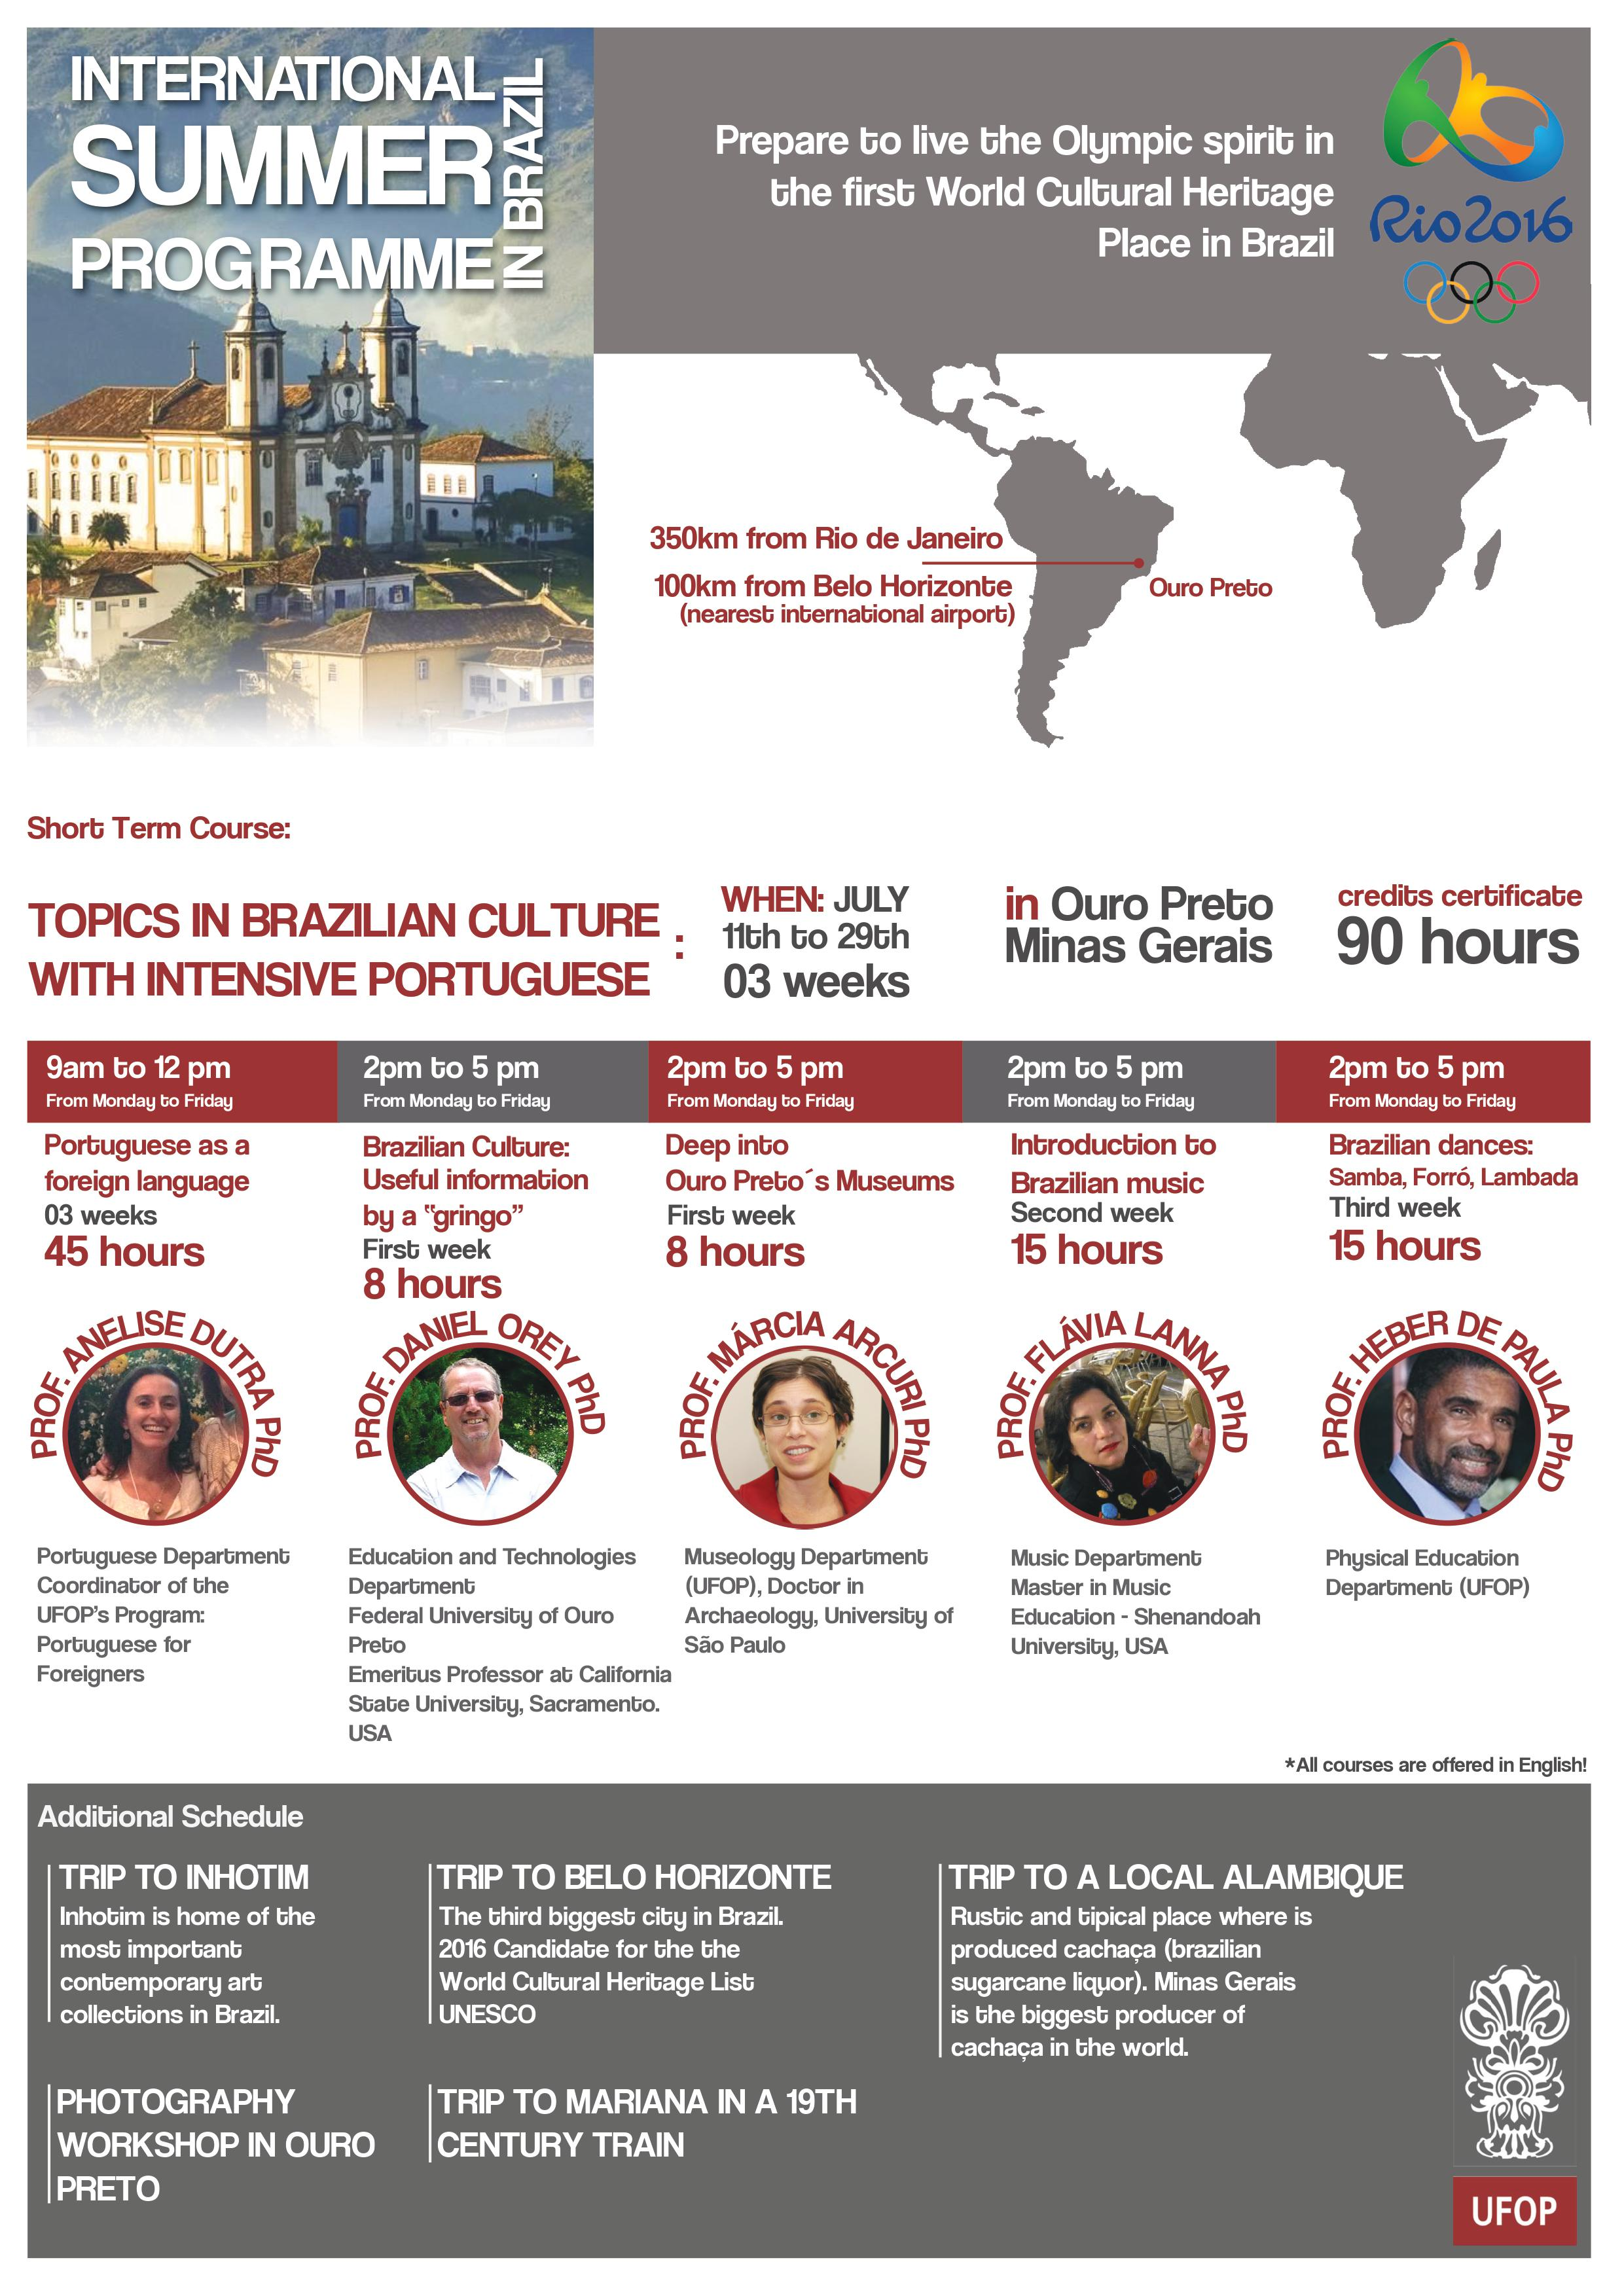
\includegraphics[scale=0.5]{figuras/Summer_Course1.jpg}
%	\caption{Primeiro programa de recepção de discentes estrangeiros.}
%	\label{fig:01}
%\end{figure}
%

\section{Campus em Números}
%
Em uma estrutura \textit{multicampi}, formada pelos \textit{campi} de Ouro Preto, Mariana e João Monlevade, a universidade está inserida na mesorregião de Belo Horizonte, estendendo-se até João Monlevade, e na microrregião de Ouro Preto, que abrange as cidades de Itabirito, Ouro Preto, Mariana, Diogo de Vasconcelos e Acaiaca. Essa microrregião abarca, conforme dados do IBGE,\footnote{\url{https://cidades.ibge.gov.br/}} uma população de aproximadamente $197.424$ habitantes, uma Universidade, dois Institutos Federais, $118$ unidades escolares de ensino fundamental, $28$ escolas com ensino médio, apresentando as escolas um público de cerca de $2318$ profissionais da educação e $31492$ discentes, o que demanda da UFOP uma importante inserção acadêmica e reconhecimento na região.

Atualmente, a Universidade, incluindo os 3 campi, ocupa uma área de aproximadamente $649.740$ $m^2$, com $356$ laboratórios e $256$ salas de aulas. Considerando um levantamento feito em agosto de 2022, a UFOP conta com $915$ professores efetivos e $698$ técnicos-administrativos. Oferece $56$ cursos de graduação, sendo quatro na modalidade à distância: Pedagogia, Administração Pública, Licenciatura em Geografia e Licenciatura em Matemática. Em relação à pós-graduação, são ofertados $16$ programas de doutorado, $27$ de mestrado acadêmico e $9$ de mestrado profissional além de e $9$ cursos de especialização lato sensu. Quanto ao corpo discente, são $13.343$ discentes(as) de graduação, $797$ deles(as) matriculados(as) na modalidade a distância. Na pós-graduação, são $556$ matrículas em programas de doutorado; $1.505$ em programas de mestrado, dos quais $1222$ são em mestrado acadêmico e $283$ em mestrado profissional além de aproximadamente $293$ matrículas em programas de especialização (presencial e a distância).\footcite[De acordo com o plano de desenvolvimento institucional (PDI) aprovado para o período $(2016-2025)$, por meio da resolução CUNI 1793 de 14 de dezembro de 2015. Ver em][]{PDI-UFOP} Uma considerável diversidade, especialmente para o calouro que aporta pela primeira vez em Ouro Preto.

\section{Contexto Nacional, Regional e local}
%
Segundo dados da Sinopse Estatística da Educação Superior do ano de 2018 (INEP, 2018), o Brasil possui 2.537 Instituições de Ensino Superior, sendo 107 Universidades públicas, destas 63 Federais, 40 Estaduais e 4 Municipais. O estado de Minas Gerais contribui com 307 Instituições de Ensino, em que 22 são Universidades, sendo 13 públicas, onde 11 são Universidades Federais e 2 Estaduais.

Ainda de acordo com dados INEP coletados no ano de 2020, a partir do Senso da Educação Superior no Brasil, 41.953 cursos na modalidade de graduação já eram ofertados no Brasil, com mais de 19 milhões de vagas anuais. Esse dado indica que a oferta de cursos de evoluiu de maneira ascendente ao longo do período de 2011 a 2020, partindo de 30.420, em 2011, e alcançando 41.953 cursos, o correspondente a um crescimento geral de 37,9\%:\footcite[][p.~17]{senso-inep}
\begin{quotation}
``...~Em 2020 foi ofertado o total de 19.626.441 vagas, das quais 68,9\% a distância e 31,1\% presenciais. Além disso, 95,6\% das vagas foram ofertadas na categoria privada, contra 4,4\% ofertadas na categoria pública. Vale dizer que, do total de vagas presenciais, 11,9\% são públicas e 88,1\% são privadas; das vagas a distância, 1,0\% são públicas e 99,0\% são privadas. Considerando o tipo de vagas, tem-se a seguinte distribuição total: 73,0\% de vagas novas, 26,7\% de vagas remanescentes e 0,3\% de vagas em programas especiais.''
\end{quotation}

A representatividade das Instituições corresponde a mais de 863.520 cursos
8 milhões de discentes matriculados, divididos nas esferas pública (2.077.481 matrículas) e privada (6.373.274 matrículas). O estado de Minas Gerais possuía 208.340 discentes em Instituições públicas e 643.814 discentes em Instituições privadas, correspondendo a cerca de 10\% de absorção de discentes matriculados em IES no Brasil, tanto na rede pública como privada.

Com relação a oferta de cursos, segundo dados do  INEP de 2020,\footcite[][]{senso-inep} são 1.687 instituições (na modalidade pública) que oferecem 6.522 cursos na área de Engenharia, Produção e Construção. A Engenharia de Controle e Automação é oferecida em 160 Instituições e com 203 cursos distintos. Especificamente com relação ao curso de Engenharia de Controle e Automação da UFOP, pode-se afirmar que ele foi delineado de acordo com as Diretrizes Curriculares Nacionais (DCN), com os princípios institucionais estabelecidos no PDI e PPI da UFOP, levando-se também em consideração a relação com as atividades econômicas do município de Ouro Preto e suas necessidades industriais. Atualmente, a realidade econômica da região do Quadrilátero Ferrífero tem suas bases fortemente relacionadas ao turismo e na indústria de transformação e reservas minerais do seu subsolo, tais como ferro, bauxita, manganês, talco e mármore.

A cidade histórica de Ouro Preto é famosa por sua arquitetura colonial e pelo clima peculiar, que dá um charme especial à cidade. Situada a uma altitude média de 1.179 metros, abriga uma população de mais de 70.000 habitantes, conforme o censo de 2010 do Instituto Brasileiro de Geografia e Estatística (IBGE). Com mais de 300 anos de história, Ouro Preto é um dos principais símbolos de Minas Gerais, e não só entre os limites do país, mas também no exterior. A antiga Vila Rica, no passado berço de alguns dos mais importantes movimentos na luta pela independência brasileira e hoje palco de grandiosos eventos culturais, é um dos ícones máximos do Barroco nacional e mundial. A cidade, tombada como Patrimônio Histórico e Cultural da Humanidade, título conferido pela Organização das Nações Unidas (Unesco), é berço de escritores, artistas e toda sorte de personalidades. Mas, sobretudo, Ouro Preto é conhecida por ser uma cidade eminentemente universitária.

Os estudantes da UFOP procedem principalmente dos estados de Minas Gerais, São Paulo, Rio de Janeiro, Espírito Santo e Goiás. Uma realidade que foi sendo alterada gradativamente ao longo dos últimos $20$ anos, período em que a universidade aderiu às novas formas de gestão da educação implementadas em âmbito nacional. Excetuando-se os discentes provindos das escolas federais de esino médio, técnico e tecnológico, percebeu-se um aumento significativo de egressos das escolas públicas da chamada ``região dos Inconfidentes''(Ouro Preto, Mariana e arredores), sobretudo aqueles de Escolas públicas estaduais, que eram raros há alguns anos atrás, especialmente aqueles advindos de classes sociais menos favorecidas. Isto não significa, entretanto, que a realidade da educação pública, sob a ótica do ensino médio, tenha se alterado de forma que o acesso à universidade pública fosse facilitado. A política de cotas e projetos de extensão voltados para ensino e reforço no ensino médio (oferecidos pelas próprias Universidades) são iniciativas que contribuíram para o maior acesso à Universidade pública por estudantes de famílias de baixa renda.
%
%E viver como estudante em Ouro Preto significa, quase sempre, a sua integração em uma das marcas da cultura universitária da cidade: as ``repúblicas estudantis'', que são um tópico à parte. As repúblicas fazem parte da tradição da cidade. Muitas delas instaladas em prédios históricos, pertencentes à Universidade Federal de Ouro Preto (sendo simplesmente denominadas como ``Repúblicas Federais''), absorvem parcela significativa dos estudantes, tanto em Ouro Preto quanto Mariana. São administradas pelos próprios estudantes, que definem suas regras de admissão. Ao longo de mais de um século, as repúblicas desenvolveram uma cultura própria e mantêm laços estreitos com ex-discentes e ex-residentes, inclusive no que tange à rede de contatos profissionais. Esse laço é muito forte entre as repúblicas federais e mesmo entre as chamadas ``repúblicas particulares'' (que não pertencem à universidade), especialmente na condução das famosas e tradicionais ``festas republicanas'': 12 de outubro, aniversário da Escola de Minas e o 21 de abril, dia de Tiradentes e aniversário das Repúblicas do Campus. Nestes períodos, os antigos ex-discentes costumam marcar presença como uma forma de relembrar e reviver as lembranças dos tempos de universidade. A Refop (Associação das Repúblicas Federais de Ouro Preto) é composta por $67$ repúblicas, sendo uma mista, $51$ masculinas e $15$ femininas. Os discentes veteranos e muitos ex-discentes atestam que a estrutura que existe entre os moradores de uma república são fundamentais para a sua formação como futuros profissionais, especialmente em um contexto de mundo globalizado.
%%%%%%%%%%%%%%%%%%%%%%%%%%%%%%

\chapter{Informações sobre o curso}
%
\begin{itemize}
    \item[] Nome da Instituição: Universidade Federal de Ouro Preto
	\item[] Nome do Curso: Engenharia de Controle e Automação;
	\item[] Modalidade: (X) presencial ( ) À distância
	\item[] Turnos de funcionamento: ( ) manhã ( X ) vespertino ( X ) noturno
	\item[] Endereço de funcionamento: Campus Morro do Cruzeiro s/n, Bairro Bauxita, Ouro  Preto-MG, 35.400-000;
	\item[] Unidade Acadêmica: Escola de Minas;
	\item[] Atos legais de autorização:
	\begin{itemize}
	    \item Resolução CEPE 1611 de 08/11/1999: autorização de criação do curso;
	    \item Portaria $N^{o}$ 111, DE 4 DE FEVEREIRO DE 2021: renovação de reconhecimento de curso.
	\end{itemize}
	\item[] Titulação conferida aos egressos: Engenheiro de Controle e Automação;
	\item[] Número de vagas oferecidas: 36 por semestre;
	\item[] Regime de matrícula: ( ) anual (X) semestral;
	\item[] Área de conhecimento:
	\begin{itemize}
	    \item Grande área: Engenharias IV
	    \item Área específica: Engenharia Elétrica
	\end{itemize}
	\item[] Tempo regular e máximo de  integralização (anos e
	semestres letivos): 5 anos (ou 10 semestres) e 7,5 anos (ou 15 semestres);
	\item[] Conceito Preliminar do curso  (CPC): 4 (2014)
	\item[] Nota do Enade: 4 (2014), 3 (2017)
\end{itemize}

\section{Histórico do Curso}
%
A história do ramo no Brasil data de 1953, quando o Instituto Tecnológico de Aeronáutica (ITA) ministrou, pela primeira vez, um curso de controle automático. Desde então, a área de Automática -- termo criado para designar a ciência e a Engenharia de Controle e Automação no Brasil -- desenvolveu-se rapidamente nas universidades brasileiras, destacando-se os cursos de controle de sistemas dinâmicos da USP e Unicamp, já no início dos anos $1970$.

Atualmente, existem cursos de engenharia associados a sistemas mecatrônicos nos Estados Unidos, no Canadá, na Europa e na Ásia. Ciente da necessidade e da relevância de se formar engenheiros de Controle e Automação no Brasil, o Ministério da Educação, através da Portaria $1.694$, de $5$ de dezembro de $1994$, publicada no Diário Oficial da União de $12$ de dezembro de $1994$, considerando o consubstanciado no parecer da Comissão de Especialistas do Ensino de Engenharia da Secretaria de Educação Superior, regulamentou a Engenharia de Controle e Automação.

Diversas universidades brasileiras oferecem cursos associados a sistemas mecatrônicos, como os cursos oferecidos pela Escola Politécnica da Universidade de São Paulo, o curso de Engenharia de Controle e Automação da Universidade Estadual de Campinas, o curso de Engenharia Mecânica com ênfase em Automação e Sistemas da Escola de Engenharia de São Carlos da Universidade de São Paulo, o curso de Engenharia de Controle e Automação da Universidade Federal de Santa Catarina, o curso de Engenharia de Controle e Automação da Universidade Federal de Minas Gerais, o curso de Engenharia Mecânica com ênfase em Mecatrônica e o curso de Engenharia de Controle e Automação da Pontifícia Universidade Católica de Minas Gerais, o curso de Engenharia de Controle e Automação da Universidade de Brasília e o curso de Engenharia de Controle e Automação da Universidade Federal de Itajubá.

Na Universidade Federal de Ouro Preto, o curso de Engenharia de Controle e Automação foi concebido no final da década de $1990$ de forma a responder às necessidade de expansão da própria instituição (e também do mercado), face aos novos tempos. Sabia-se, até aquele momento, que a universidade possuía contribuições significativas para o desenvolvimento da engenharia no Brasil, especialmente pela tradição centenária da Escola de Minas. Assim, em agosto do ano $2000$, iniciam-se as primeiras turmas do curso de graduação em Engenharia de Controle e Automação na UFOP. Vale mais uma vez ressaltar que o curso foi o campeão de inscrições na universidade, quando aberto o primeiro vestibular.

Sob a ótica industrial, não é despropositado afirmar que há, ainda, escassez de profissionais com essa formação no país. Segundo informações do guia do estudante de $2016$,\footcite{guia-do-estudante} os setores de petróleo e gás, manufatura, mineração e metalurgia são tradicionais empregadores. Três novas áreas apresentam grande potencial: indústria portuária, robótica e a domótica (pesquisa e desenvolvimento de automação de rotinas e tarefas domésticas). Empresas automobilísticas também demandam o graduado. O Sul, o Sudeste e a região da Zona Franca de Manaus são os principais centros de emprego ao longo do país. Na região de maior atuação da universidade federal de Ouro Preto, os grandes empregadores são as empresas de mineração, metalurgia e as de base tecnológica situadas na região metropolitana de Belo Horizonte.

Pode-se inclusive, ressaltar a crescente importância da Engenharia de Controle e Automação para os setores de:
\begin{itemize}
	\item Conservação do patrimônio histórico;
	\item Iluminação e Energia (Energias renováveis);
	\item Automobilístico (eletrificação automotiva, veículos autônomos);
	\item Robótica e Internet 4.0 (Internet das Coisas ou \textit{IoT});
	\item Serviços (Automação comercial, automação do sistema bancário);
	\item Construção Civil (Automação predial);
	\item Tecnologias assistivas;
	\item Agro-indústria;
	\item Sistemas de segurança, monitoramento;
	\item Outros.
\end{itemize}

\section{Justificativas}
As atuais demandas da sociedade por bens e serviços têm sido cada vez mais atendidas utilizando-se de novas tecnologias, resultantes da aplicação do conhecimento científico. Isto não é diferente no microclima da região dos inconfidentes, principal ``cliente'' da universidade. O ensino de engenharia em face dessa realidade passa por grandes mudanças, com a criação de novas habilitações, a concepção e adaptação de novos currículos e estratégias pedagógicas, com o objetivo de formar engenheiros capazes de desenvolver, aperfeiçoar e utilizar as novas tecnologias de base científica. Com o grande desenvolvimento da eletrônica, da informática e das comunicações nas últimas décadas, uma das áreas mais ativas da engenharia em todo mundo passou a ser, obviamente, a área de Controle e Automação, que é uma das personagens mais destacadas na reconhecida revolução que está  em curso: a Indústria 4.0. Portanto, pode-se afirmar que tal curso oferece uma vantagem  significativa tanto do ponto de vista estratégico quanto econômico para a UFOP.

Além disso, desde a criação da graduação em Engenharia de Controle e Automação, que agora possui mais de duas décadas de história, poucas alterações haviam ocorrido em seu  arcabouço. Isto vai na contramão de um mundo que se alterou rapidamente, em termos científicos, econômicos e tecnológicos no mesmo período. Após a divulgação, por parte da  PROGRAD da UFOP de um programa de restruturação chamado Plano de Ações  Pedagógicas (PAP) em 2014, surgiu a necessidade de se rediscutir toda a base da graduação  em Engenharia de Controle e Automação. Isto passa pela rescrita de todo o projeto de  curso e não apenas sua atualização. Dada a magnitude do trabalho a ser realizado, as  discussões se estenderam desde 2014, quando das primeiras discussões, até hoje, \today, ocasião em que este documento foi revisto e atualizado pela última vez.

A reformulação do PPC e da matriz curricular teve como base o Plano de Desenvolvimento Institucional da UFOP (PDI) e o Projeto Pedagógico Institucional da UFOP (PPI). A recomposição é oportuna por entender que as tecnologias emergentes e as inovações generalizadas são difundidas muito mais rápida e amplamente que as anteriores,  ademais, certifica o atendimento às Resoluções do Conselho Nacional de Educação/Câmara de Educação Superior (CNE/CES) nº. 7, de 18 de dezembro de 2018, que estabelece as Diretrizes para a Extensão na Educação Superior Brasileira, a Resolução CNE/CES nº. 2, de 24 de abril de 2019, no qual institui as Diretrizes Curriculares Nacionais do Curso de Graduação em Engenharia e os novos instrumentos de avaliação do SENAES/INEP.

\section{Objetivos do Curso}
%
\subsection{Objetivos Gerais}
O discente depois de formado deverá ter forte base científica e profissional, bem como conhecimentos técnicos em diversas áreas de engenharia, notadamente elétrica, eletrônica, mecânica e computação. A sua formação técnico-científica e profissional deverá ser ampla e geral, de forma a capacitá-lo a absorver, avaliar criticamente e desenvolver novas tecnologias, estimulando a sua atuação criativa na identificação e resolução dos mais diversos problemas, considerando suas diferentes dimensões sociais. As atividades de ensino, pesquisa e extensão oferecidas no curso, além de diversos eventos acadêmicos, também possibilitam ao estudante o desenvolvimento de outras habilidades tão importantes quanto as técnicas como: comunicação, gestão de tempo, flexibilidade, adaptabilidade, trabalho em equipe, saber lidar com pressão e suportar críticas, ter atitude positiva e autoconfiança. Isso permite um amplo espectro de atuação profissional desse egresso. Tal formação deve ser coerente e compatível com as habilitações profissionais definidas pelo sistema CONFEA-CREA.

\subsection{Objetivos Específicos}
Objetiva-se formar um engenheiro com habilidades e competências para concepção e manutenção de sistemas de controle de processos industriais e automação, aplicação consciente com avaliação crítica de métodos e ferramentas de engenharia no projeto, integração e dimensionamento de dispositivos de controle automático e células automatizadas de produção, gerenciamento e execução de projetos de automação de processos industriais, bem como desenvolvimento de pesquisa científica e tecnológica, apto a atuar tanto em indústrias usuárias de tecnologias de automação industrial e sistemas de controle automáticos como de produção de equipamentos e \textit{software} para automação industrial, em empresas de prestação de serviços em engenharia próprias ou de terceiros.


\section{Perfil e Competência Profissional do Egresso}
%
Poder-se-ia dizer que a formação do engenheiro de controle e automação encerra um caráter
abrangente de atuação na natureza e, por este motivo, tem como pedra fundamental a integração entre diversas áreas do conhecimento humano, desde a matemática, a física, a química e as ciências da computação. No entanto, sua atuação não se restringe a tais campos do saber, podendo dar-se em inumeráveis outros campos, o que torna difícil a tarefa de enquadrá-lo nas tradicionais áreas da engenharia, como elétrica, eletrônica, mecânica ou computação.

No nosso caso específico, pode-se afirmar que desde a criação do curso em 1999, muitos desafios foram superados. Identificou-se como sendo um dos principais deles, especialmente no que concerne ao perfil dos egressos, o da formação específica para a atuação em empresas, destacando-se aquelas do setor minero-metalúrgico. Tal justificativa dava-se pela vocação da própria região e necessidades do mercado. No entanto, passadas duas décadas de existência, detectou-se a necessidade de expansão de conceitos, de forma a contribuir na formação de engenheiros com perfil mais abrangente e empreendedor, dentro de uma perspectiva holística, ética e humanista, e não apenas para suprir demandas mercadológicas.

Com o rápido desenvolvimento do campos da inteligência artificial e da automação, a atual revolução tecnológica tem levado a rápidas mudanças nas relações e postos de trabalho. Dessa forma, não é mais possível, hoje, fazer previsões de como estará o mercado de trabalho dentro dos próximos 20 anos. Assim, o curso de Engenharia de Controle e Automação da UFOP deve focar no desenvolvimento de competências que possibilitem ao egresso ser flexível o suficiente para se adaptar e até mesmo para ser promotor de mudanças no mercado de trabalho. Um egresso capaz de pensar novas soluções, adquirir novas habilidades e, enfim, de continuar se aperfeiçoando e se reinventado de modo a promover o desenvolvimento pessoal mas, sobretudo, da sociedade em que está inserido, de forma responsável e sustentável.
%
\chapter{Estrutura Administrativa}
\label{cap:03} \index{administracao}

\section{Estrutura Administrativa}
A Universidade é estruturada de acordo com o  seu estatuto, aprovado na Resolução CUNI 1868 de 17 de fevereiro de 2017\footcite{resolucao-cuni-1868}, que estabeleceu a sua organização da seguinte forma:
\begin{itemize}
    \item Conselho Universitário (CUNI), assessorado por:
    \begin{itemize}
      \item Câmara de Pessoas;
      \item Câmara de Infraestrutura;
      \item Câmara de Orçamento e Finanças.
    \end{itemize}
    \item Conselhos Superiores
    \begin{itemize}
        \item Conselho Superior de Graduação;
        \item Conselho Superior de Pesquisa e Pós-Graduação;
        \item Conselho Superior de Extensão e Cultura.
    \end{itemize}
    \item Conselho Curador (CONC)
    \item Reitoria
    \item Unidades Acadêmicas
    \item Conselhos das Unidades
    \item Colegiados de Cursos
    \item Departamentos
\end{itemize}

No âmbito administrativo, a responsabilidade máxima é exercida pela Reitoria, competindo à Vice-Reitoria colaborar com ela nas funções a ela delegadas e substituí-la, automaticamente, nos casos de falta, de impedimento ou de vacância.

É responsável pela proposição, coordenação e acompanhamento da política de graduação da UFOP. É também a instância encarregada dos processos seletivos e do gerenciamento acadêmico dos cursos de graduação.

De acordo com o Art. 36 do Estatuto da UFOP, as Unidades Acadêmicas Universitárias são os órgãos que administram o exercício simultâneo de atividades de ensino, pesquisa e extensão em uma ou mais áreas de conhecimento, respeitadas as normas legais, estatutárias, regimentais e as resoluções dos órgãos competentes, compondo sua estrutura as unidades de Ouro Preto, Mariana e João Monlevade. No âmbito das Unidades acadêmicas, os órgãos deliberativos e consultivos são os Conselhos das Unidades, os Colegiados de Curso e os Departamentos.
%
\section{Colegiado do Curso}
A UFOP se organiza a partir da reitoria, pró-reitorias, órgãos suplementares, unidades acadêmicas, departamentos de docentes e colegiados de cursos de graduação e pós-graduação. Assim, existe a Pró-Reitoria de Graduação, responsável por regulamentar as normas de graduação da Universidade. Existe também a Unidade Acadêmica, que compreende os departamentos e colegiados de curso que são originários dessa unidade.

Cada curso de graduação da UFOP possui seu Colegiado de Curso, o qual é constituído por representantes dos Departamentos que oferecem disciplinas no curso, eleitos pelas respectivas Assembleias, em proporção ao número de créditos das disciplinas ministradas, com mandato de dois anos, permitida uma recondução.

De acordo com o Art. 49 do Estatuto da UFOP compete aos Colegiados:

\begin{quotation}
I - compatibilizar as diretrizes gerais dos componentes curriculares do respectivo curso e estabelecer as modificações necessárias;

II - regulamentar os componentes curriculares do curso para execução do seu projeto
pedagógico;

III - - deliberar sobre as ementas e os programas elaborados pelas unidades, relativos ao ensino das várias disciplinas, para fim de organização do projeto pedagógico do curso;

IV - propor à aprovação dos Conselhos Superiores o projeto pedagógico do curso e suas
alterações, com indicação dos pré-requisitos, da carga horária, das ementas, dos programas, dos regulamentos e dos componentes curriculares que o compõem;

V - decidir sobre questões relativas à reopção de cursos, equivalência de disciplinas, desligamento, jubilamento, aproveitamento de estudos, ingresso de portador de diploma de graduação, transferência, reingresso e mobilidade acadêmica nacional e internacional;

VI - apreciar as recomendações das Unidades Acadêmicas e os requerimentos dos
docentes sobre assunto de interesse do curso;

VII - coordenar a orientação acadêmica dos estudantes do curso, com vistas à
integralização curricular e colação de grau;

VIII – indicar às Pró-Reitorias competentes os candidatos à colação de grau e ou
diplomação;

IX - indicar, no caso dos colegiados dos cursos de graduação, os membros do Núcleo
Docente Estruturante do Curso ou órgão similar, podendo os representantes indicados serem ou não membros do Colegiado;

X - recomendar ao departamento ou à organização de nível hierárquico equivalente a que esteja vinculado, o componente curricular, as providências necessárias à melhor utilização das instalações, do material e do aproveitamento do pessoal, bem como abertura de vagas e de turmas.
\end{quotation}

%Na página do Departamento do curso de Engenharia de Controle e Automação,\footnote{\url{decat.ufop.br}.} é possível encontrar as principais informações sobre o curso, as Resoluções CEPE e CECAU que tratam das regras de monografia e estágios, informações sobre as Atividades Acadêmico-Científico-Culturais (AACC) além de outras informações de interesse pedagógico e operacional do curso de Engenharia de Controle e Automação. O presidente do Colegiado, que sempre será um professor, tem o papel de coordenar as atividades acadêmicas e pedagógicas do curso.

%A composição do Colegiado do Curso de Engenharia de Controle e Automação é apresentada:

%Presidência do Colegiado
%Profa. Luciana Gomes Castanheira / Mandato iniciado em março/2018
%Email: luciana.castanheira@ufop.edu.br

%Secretário do Colegiado
%Sr. Matias Alves Silva
%Email: cecau.em@ufop.edu.br
%Telefone: 3559-1542

Os colegiados de curso de graduação trabalham em parceria com seu Núcleo Docente Estruturante (NDE), órgão que contribui em temas que diz respeito ao acompanhamento e atuação nos processos de concepção, consolidação e contínua atualização do projeto pedagógico do curso bem como outras atividades que julgar importantes para o bom andamento do curso.

\section{Núcleo Docente Estruturante}
%
O Núcleo Docente Estruturante foi um conceito criado pela portaria n◦147 de 2 de fevereiro de 2007, do Ministério da Educação, com o intuito de qualificar o envolvimento docente no processo de concepção e consolidação de um curso de graduação:

\begin{quotation}
    ``...~Entende-se, então, que todo curso que tem qualidade possui (ainda que informalmente) um grupo de professores que, poder-se-ia dizer, é a alma do curso. Em outras palavras, trata-se de um núcleo docente estruturante. É importante ainda observar que, dentro da tradição bastante burocratizante das instituições de ensino no Brasil, recomendar-se ou, mais ainda, exigir-se a existência de um NDE, tenderia a induzir a definição deste como um órgão deliberativo, o que pode significar a perda da eficácia de suas funções. O NDE deve ser considerado não como exigência ou requisito legal, mas como elemento diferenciador da qualidade do curso, no que diz respeito à interseção entre as dimensões do corpo docente e Projeto Pedagógico do Curso.''
\end{quotation}

Por meio da resolução CEPE n.4450, de 29 de abril de 2011,\footcite{resolucao-cepe-4450} o Conselho de Ensino, Pesquisa e Extensão da Universidade Federal de Ouro Preto instituiu o Núcleo Docente Estruturante (NDE), nos termos da Resolução CONAES n.01/2010, de 17 de junho de 2010, com o intuito de qualificar o envolvimento docente no processo de concepção e consolidação de um curso de graduação. O NDE tem competência acadêmica de acompanhamento e de atuação nos processos de concepção, consolidação e contínua atualização do projeto pedagógico do curso.
As ações e deliberações do NDE, que devem ser referendadas pelo colegiado, englobam:

\begin{itemize}
\item Contribuir na consolidação do perfil profissional do egresso do curso;

\item Zelar pela integração curricular interdisciplinar entre as diferentes atividades de ensino constantes no currículo;

\item Indicar formas de incentivo ao desenvolvimento de linhas de pesquisa e extensão, oriundas de necessidades da graduação, de exigências do mercado de trabalho e afinadas com as políticas públicas relativas à área de conhecimento do curso; e zelar pelo cumprimento das Diretrizes Curriculares Nacionais para os Cursos de Graduação.
\end{itemize}

Os integrantes do NDE são designados por Portaria do(a) Diretor(a) da Unidade Acadêmica responsável pela oferta do curso de graduação, a partir de uma lista de professores indicados pelo Colegiado de Curso, para um mandado de três anos, permitindo-se reconduções sucessivas, caso sejam compreendidas com fator positivo para o curso. É recomendada a manutenção de pelo menos 1/3 dos membros atuais na renovação da composição. Pelo menos 60\% dos membros deve ter titulação acadêmica stricto sensu e 20\% dos membros com regime de trabalho em tempo integral e a presidência será exercida por um de seus membros eleito pelos seus pares.

Ao NDE cabe a manutenção do presente Projeto Pedagógico de Curso (PPC) e a correspondente implementação. O NDE é um órgão consultivo, cujas sugestões e decorrentes ações devem ser avaliadas e aprovadas pelo Colegiado de Curso de Engenharia de Controle e Automação, que é o órgão deliberativo. Este grupo deve avaliar constantemente o andamento do Curso, especialmente nos primeiros anos, propondo melhorias e ajustes no PPC que impactem no bom funcionamento do Curso, de forma a possibilitar a realização dos objetivos propostos.

\section{Corpo Docente e Administrativo}
%
O curso de Engenharia de Controle e Automação está instalado na Escola de Minas, sendo vinculado ao departamento de Engenharia de Controle e Automação (DECAT). %, responsável pelas áreas de concentração em Controle de Processos Industriais e Automação de Processos.

Além deste departamento, há a participação de outros departamentos da UFOP, que oferecem disciplinas ao Curso de Engenharia de Controle e Automação, sendo eles: Departamento de Engenharia Mecânica (DEMEC), Departamento de Engenharia de Minas (DEMIN), Departamento de Engenharia Metalúrgica (DEMET), Departamento de Engenharia de Produção (DEPRO), Departamento de Arquitetura e Urbanismo (DEARQ), Departamento de Engenharia Civil (DECIV), Departamento de Ciências da Computação (DECOM), Departamento de Matemática (DEMAT),  Departamento de Física (DEFIS),  Departamento de Química (DEQUI), Departamento de Educação (DEEDU), Departamento de Filosofia (DEFIL), Departamento de Gestão Pública (DEGEP), Departamento de Engenharia Ambiental (DEAMB), Departamento de Estatística (DEEST) e Departamento de Direito (DEDIR).

%O curso de Engenharia de Controle e Automação está instalado na Escola de Minas – EM, sendo vinculado, nas áreas de concentração/ênfase, aos departamentos de:
%\begin{itemize}
%	\item Engenharia de Controle e Automação e Técnicas Fundamentais (DECAT) – responsável pelas áreas de concentração em Controle de Processos Industriais: Mineração e Metalurgia e em Automação de Processos;
%	\item Computação (DECOM) – participação, com oferecimento de disciplinas específicas, nas áreas de concentração citadas acima;
%	\item Engenharia de Minas (DEMIN) – participação, com oferecimento de disciplinas específicas, na área de concentração em Controle de Processos Industriais: Mineração e Metalurgia;
%	\item Engenharia Metalúrgica e de Materiais (DEMET) - participação, com oferecimento de disciplinas específicas, na área de concentração em Controle de Processos Industriais: Mineração e Metalurgia.
%\end{itemize}

%Além destes departamentos há a participação de outros Departamentos da UFOP, como o Departamento de Matemática (DEMAT), o Departamento de Física (DEFIS), o Departamento de Química (DEQUI), pertencentes ao Instituto de Ciências Exatas e Biológicas, o Departamento de Educação (DEEDU), pertencente ao Instituto de Ciências Humanas e Sociais, o Departamento de Filosofia (DEFIL), pertencente ao Instituto de Filosofia, Arte e Cultura, o Departamento de Direito (DEDIR), e também dos Departamentos de Engenharia de Produção, Administração e Economia (DEPRO) e de Engenharia Civil (DECIV) da Escola de Minas que oferecem disciplinas do Curso de Engenharia de Controle e Automação.

Nas tabelas \ref{tab:0301} e \ref{tab:0302} destacam-se a relação de Docentes efetivos e de Técnicos Administrativos em Educação (TAE) do Departamento de Engenharia de Controle \& Automação e Técnicas Fundamentais (DECAT).

% DOCENTES
\begin{table}[]
\caption{Servidores e servidoras Docentes}
\label{tab:0301}
\resizebox{\textwidth}{!}{%
\begin{tabular}{@{}lllll@{}}
\toprule
 &
  Nome &
  Título &
  Área de atuação &
  Linha de Pesquisa \\ \midrule
1 &
  Adrielle de Carvalho Santana &
  Doutora &
  Engenharia Elétrica &
  \begin{tabular}[c]{@{}l@{}}Sinais e sistemas, Internet das coisas \\ Inteligência computacional, Instrumentação \\ Circuitos eletrônicos e Engenharia biomédica.\end{tabular} \\
2 &
  Agnaldo José da Rocha Reis &
  Doutor &
  Controle e Automação &
  \begin{tabular}[c]{@{}l@{}}Instrumentação Industrial, Inteligência Computacional.\end{tabular} \\
3 &
  Alan Kardek Rego Segundo &
  Doutor &
  Engenharia Agrícola &
  \begin{tabular}[c]{@{}l@{}}Sistemas Embarcados \\ Instrumentação.\end{tabular} \\
5 &
  Danny Augusto Vieira Tonidandel &
  Doutor &
  Engenharia Elétrica &
  \begin{tabular}[c]{@{}l@{}} Sistemas a Eventos Discretos \\ História da Eletricidade e do Controle Automático \\ \end{tabular} \\
12 &
  João Carlos Vilela de Castro &
  Doutorando &
  Engenharia Elétrica &
  Sistemas de Controle. \\
13 &
  José Alberto Naves Cocota Junior &
  Doutor &
  Engenharia de Materiais &
  \begin{tabular}[c]{@{}l@{}}Robótica, Controle de Processos, Automação Industrial.\end{tabular} \\
14 &
  Karla Boaventura P. Palmieri &
  Doutor &
  Controle e Automação &
  \begin{tabular}[c]{@{}l@{}}Automação Industrial e Robótica \\ Sistemas de Manufatura.\end{tabular} \\
15 &
  Luciana Gomes Castanheira &
  Doutora &
  Engenharia de Materiais &
  Redes Neurais e Automação Industrial. \\
23 &
  Paulo Marcos de Barros Monteiro &
  Doutor &  Engenharia Agrícola & Controle de Processos e Iluminação.
   \\
24 &
  Regiane de Sousa Silva Ramalho &
  Mestre &
  Engenharia Elétrica &
  \begin{tabular}[c]{@{}l@{}}Acionamento e Maquinas Elétricas \\ Automação Industrial \\ Redes Industriais.\end{tabular} \\
25 &
  Bruno Nazário Coelho &
  Doutor &
  Engenharia de Materiais &
  \begin{tabular}[c]{@{}l@{}}Sistemas de Automação e Controle\\ Automação eletrônica de processos elétricos e industriais.\end{tabular} \\
26 &
  Bruno Randazzo Baroni &
  Doutor &
  Engenharia Elétrica &
  Máquinas Elétricas \\ \bottomrule
\end{tabular}%
}
\end{table}

% TAES
\begin{table}[]
\caption{Servidores TAE's do curso de Engenharia de  Controle e Automação}
\label{tab:0302}
\begin{tabular}{@{}lcl@{}}
\toprule
\rowcolor[HTML]{D9D9D9}
\multicolumn{1}{c}{\cellcolor[HTML]{D9D9D9}\textbf{Nome}} & \textbf{Área} & \multicolumn{1}{c}{\cellcolor[HTML]{D9D9D9}\textbf{Cargo}} \\ \midrule
Diógenes Viegas Mendes Ferreira & Controle e Automação & Técnico Efetivo \\
Fernando dos Santos Alves       & Controle e Automação & Técnico Efetivo \\
Francisco de Paula Coelho       & Controle e Automação & Técnico Efetivo \\
José Gonçalves Arruda           & Controle e Automação & Técnico Efetivo \\
Robson Nunes Dal Col            & Controle e Automação & Técnico Efetivo \\
Roberta Kelly Barbosa           & Administrativa       & Técnica Efetiva \\ \bottomrule
\end{tabular}%

\end{table}


\chapter{Organização curricular}
\label{cap:04} \index{currículo}
%
A organização curricular do curso de graduação em Engenharia de Controle e Automação da Universidade Federal de Ouro Preto segue as Diretrizes Curriculares Nacionais (DCN) dos Cursos de Engenharia estabelecidas na Resolução CNE No2/2019,\footnote{Publicada no D.O.U. de 20 de Dezembro de 2019.} bem como a Resolução CNE No1/2021, que altera o Art. 9°, § 1o da Resolução CNE/CES 2/2019\footnote{Publicada no D.O.U. em Maio de 2021.} e a Política Institucional de Formação para os Cursos de Engenharia da UFOP (Resolução CUNI No2544/2022). As disciplinas e atividades presentes na matriz curricular foram organizadas de forma a atender aos objetivos e perfil profissional do egresso, descritos no item 2 deste Projeto Pedagógico de Curso. A tabela \ref{tab:0401} resume a proposta de organização dos componentes curriculares do curso de Engenharia de Controle e Automação da UFOP.
%
\begin{table}[ht]
	\caption{Organização dos Componentes curriculares}
	\label{tab:0401}
	\resizebox{0.9\textwidth}{!}{%
		\begin{tabular}{@{}lcc@{}}
			\rowcolor[HTML]{FFFFFF}
			\multicolumn{1}{c}{\cellcolor[HTML]{FFFFFF}\textbf{Componentes Curriculares}} & \textbf{Quantidade} & \textbf{Carga Horária} \\
			Disciplinas Obrigatórias                & 52          & 2910          \\
			Disciplinas Eletivas                    & 3           & 180           \\
			Estágios                                & 1           & 160           \\
			Trabalho de Conclusão de Curso          & 2           & 200           \\
			Atividades Acadêmico-Científico-Cultural (AACC) & -           & 105           \\
			Atividades Acadêmico-Científico-Cultural Extensionistas (AACCE)    & 1    & 165  \\
			\rowcolor[HTML]{FFFFFF}
			\textbf{TOTAL}                          & \textbf{59} & \textbf{3600}
		\end{tabular}%
	}
\end{table}

Dentre as disciplinas que serão apresentadas, todas são ofertadas na modalidade presencial.

O curso de Engenharia de Controle e Automação deve contemplar os seguintes conteúdos básicos: Administração e Economia; Algoritmos e Programação; Eletricidade; Estatística; Expressão Gráfica; Fenômenos de Transporte; Física; Informática; Matemática; Metodologia Científica e Tecnológica e Química, que são facilmente identificados na nossa Matriz Curricular. Outros conteúdos básicos obrigatórios são Ciência dos Materiais; Ciências do Ambiente e Mecânica dos Sólidos, que são apresentados em disciplinas como Engenharia Ambiental, Resistência dos Materiais e Processos de Metalurgia. Há ainda a formação complementar, que garante a oportunidade de projetos de pesquisa, extensão, monitoria, disciplinas eletivas e facultativas extras, entre outras oportunidades.


Em atendimento às diretrizes nacionais para a educação em direitos humanos, o curso tem como componentes curricular obrigatório a disciplina Direito e Legislação. Tal como recomendado pelo decreto no 5.626/2005, o curso tem Libras como disciplina eletiva. Outros temas transversais, como Questões Étnico-Raciais e leitura de textos técnicos em língua inglesa, são pertinentes ao aprendizado de diferentes conteúdos, sendo abordados em alguns componentes curriculares obrigatórios, tais como: Introdução a Engenharia de Controle e Automação e Trabalho de Final de Curso. Além disso, os estudantes são constantemente incentivados a buscar esses temas transversais em disciplinas facultativas, que são aquelas que não pertencem ao currículo do curso e que o estudante pode cursar durante sua permanência na Universidade. Já a temática do Desenho Universal será abordada na disciplina de Expressão Gráfica. Estas abordagens estão organizadas conforme \autoref{tab:CNE_basico} e \autoref{tab:CNE_prof}.



% Please add the following required packages to your document preamble:
% \usepackage{booktabs}
% \usepackage{graphicx}
\begin{table}[!h]
\caption{Conteúdo Básico}
	\label{tab:CNE_basico}
\resizebox{\columnwidth}{!}{%
\begin{tabular}{@{}ll@{}}
\toprule
\textbf{Disciplinas Matriz Curricular - Conteúdo Básico} & \textbf{Conteúdo Básico Definido pela CNE} \\ \midrule
Fundamentos de Programação                               & Algoritmos e Programação             \\
Algoritmos e Estrutura de Dados                          & Algoritmos e Programação             \\
Fundamentos de Mecânica                                  & Física                               \\
Fundamentos de Termodinâmica                             & Física                               \\
Fundamentos de Fluidos, Oscilações e Ondas               & Física                               \\
Fundamentos de Eletromagnetismo                          & Física                               \\
Fundamentos de Física Experimental                       & Física                               \\
Cálculo Diferencial e Integral I                         & Matemática                           \\
Geometria Analítica e Álgebra Linear                     & Matemática                           \\
Cálculo Diferencial e Integral II                        & Matemática                           \\
Introdução a Equações Diferenciais Ordinárias            & Matemática                           \\
Matemática Aplicada a Engenharia de Controle e Automação & Matemática                           \\
Química Fundamental                                      & Química                              \\
Química Experimental                                     & Química                              \\
Fundamentos de Programação                               & Informática                          \\
Algoritmos e Estrutura de Dados                          & Informática                          \\
Circuitos Digitais                                       & Informática                          \\
Estatística e Probabilidade                              & Estatística                          \\
Economia da Engenharia                                   & Administração e Economia             \\
Organização e Administração I                            & Administração e Economia             \\
Planejamento e Controle da Produção I                    & Administração e Economia             \\
Análise de Circuitos Elétricos                           & Eletricidade                         \\
Eletrotécnica para Controle e Automação                  & Eletricidade                         \\
Acionamentos Elétricos                                   & Eletricidade                         \\
Fenômenos de Transporte                                  & Fenômenos de Transporte              \\
Introdução a Engenharia de Controle e Automação          & Metodologia Científica e Tecnológica \\
Trabalho de Final de Curso I                             & Metodologia Científica e Tecnológica \\
Trabalho de Final de Curso II                            & Metodologia Científica e Tecnológica \\
Engenharia de Processos de Metalurgia                    & Ciência dos Materiais                \\
Engenharia Ambiental Básica                              & Ciências do Ambiente                 \\
Resistência dos Materiais                                & Mecânica dos Sólidos                 \\
Expressão Gráfica                                        & Desenho Universal                    \\
Introdução a Engenharia de Controle e Automação          & Questões Etnico Raciais                    \\
Cálculo Numérico                                         & Matemática / Informática             \\
Introdução ao Direito e Legislação                       & Questões Etnico Raciais
\end{tabular}%
}
\end{table}

%\,


% Please add the following required packages to your document preamble:
% \usepackage{booktabs}
% \usepackage{graphicx}
\begin{table}[!h]
\caption{Conteúdo Profissionalizante}
	\label{tab:CNE_prof}
\resizebox{\columnwidth}{!}{%
\begin{tabular}{@{}ll@{}}
\toprule
\textbf{Disciplinas Matriz Curricular - Profissionalizante} &
  \textbf{Conteúdo Básico Definido pela CNE} \\ \midrule
Introdução a Aquisição de Dados e Controle & Eletricidade/Informática             \\
Análise de Circuitos Elétricos             & Eletricidade/Física                  \\
Sistemas de Computação para Automação      & Informática                            \\
Sistemas Embutidos                         & Informática                            \\
Teoria de Controle I                       & Matemática                             \\
Teoria de Controle II                      & Matemática/Informática               \\
Teoria de Controle III                     & Matemática                             \\
Circuitos e Dispositivos Eletrônicos       & Eletricidade                           \\
Instrumentação                             & Eletricidade                           \\
Máquinas Elétricas                         & Eletricidade                           \\
Acionamentos Elétricos                     & Eletricidade                           \\
Laboratório de Contole I                   & Matemática/Informática               \\
Elementos de Robótica                      & Matemática/Informática               \\
Informática Industrial                     & Programação, Informática, Eletricidade \\
Inteligência Artificial                    & Informática                            \\
Sistemas Integrados de Manufatura          & Administração e Economia               \\
Instrumentação Inteligente                 & Eletricidade                           \\
Acionamentos Fluido Mecânicos              & Fenômenos de Transporte/Física         \\
Redes Industriais                          & Informática                            \\
Programação de Sistemas em Tempo Real      & Informática                            \\
Engenharia de Processos na Mineração &
  \begin{tabular}[c]{@{}l@{}}Fenômenos de Transporte/Mecânica dos Sólidos/\\ Ciência dos Materiais\end{tabular} \\
Engenharia de Processos na Metalurgia      & Ciência dos Materiais/Física
\end{tabular}%
}
\end{table}

A UFOP tem se destacado no cenário nacional pela institucionalização de políticas e de ações afirmativas, como por exemplo sendo a primeira universidade federal brasileira a institucionalizar uma ouvidoria feminina (Resolução CUNI No 2.249), a criar uma ouvidoria com os cargos de ouvidor e ouvidora adjunta (Resolução CUNI No 2423 ), o que faz com que questões sobre direitos humanos, relações étnico-raciais e de gênero sejam parte do cotidiano da comunidade universitária. Nesse contexto, cabe mencionar a comissão permanente de equidade, diversidade e inclusão (CPEDI) da Escola de Minas, recentemente institucionalizada.

A fim de que os estudantes tenham conhecimento não somente dessas iniciativas, mas dos vários projetos e ações em geral, em desenvolvimento na universidade, como: NEABI - Núcleo de Estudos Afro-brasileiros e Indígenas; CAIN - Coordenadoria de Acessibilidade e Inclusão; ManU - Maternidade e Universidade: ações de acolhimento e apoio às estudantes da UFOP que são mães; Andorinhas - Rede de Mulheres da Ufop; POC - Papear, Ouvir, Conscientizar; dentre muitos outros projetos, parte deles desenvolvidos através da PRACE – Pró-reitoria de assuntos comunitários e estudantis; já no programa de acolhimento aos calouros esses projetos/ações são apresentados por meio de palestras informativas com seus coordenadores e/ou membros ativos. Busca-se, assim, o envolvimento dos alunos a partir da apresentação dessas iniciativas, associada ao contínuo esclarecimento e incentivo para que estejam inteirados acerca das várias ações inclusivas em desenvolvimento na UFOP, sendo que sua efetiva participação, devidamente comprovada e estando adequada às normas específicas, podem ser computadas como CH cumprida como Atividades Acadêmico-Científico-Cultural (AACCs) ou Atividades Acadêmico-Científico-Cultural Extensionistas (AACCEs).

\section{Matriz Curricular} \label{sec:matriz}

A Matriz Curricular do curso de graduação em Engenharia de Controle e Automação da UFOP discrimina os componentes curriculares obrigatórios e complementares. Os componentes obrigatórios são compostos pelas disciplinas obrigatórias, estágio supervisionado e a Monografia. Os componentes complementares são constituídos pelas disciplinas eletivas as quais têm a função de integralizar a formação profissional do discente com conteúdo na área de Sinais e Sistemas, Automação Industrial e de Formação Geral. As disciplinas eletivas poderão ser ofertadas em inglês visando contribuir para o aprendizado do discente em um segundo idioma. O discente também deverá realizar Atividades Acadêmico-Científico-Cultural (AACC) nas quais se incluem atividades de pesquisa, projetos integradores, monitoria, entre outras e as Atividades Acadêmico-Científico-Cultural Extensionistas (AACCE).

Os componentes curriculares estão distribuídos na matriz curricular em dez períodos letivos totalizando 2910 (duas mil setecentos e noventa) horas. Adicionando-se 105 horas para AACC, 165 horas para AACCE, 160 horas para o estágio (ATV023) supervisionado e mais 80 horas para a monografia (ATV019) e 180 horas de disciplinas eletivas, o curso compreende uma carga horária total mínima de 3600 (três mil e seiscentas) horas.

%
Na próxima seção~(\ref{tab:0402}) são apresentadas as disciplinas obrigatórias distribuídas em dez períodos letivos.

\subsection{Componentes Curriculares obrigatórios}\label{tab:0402}

Nesta seção são apresentados os componentes curriculares obrigatórios, distribuídas em dez semestres letivos. O discente deve priorizar o ajuste de matrícula com as disciplinas reprovadas ou em débito. É permitido ao discente matricular-se em disciplinas posicionadas à frente do seu período de permanência, obedecendo os pré-requisitos. Conforme Resolução CEPE 3454, de 24/11/2008, o semestre letivo tem 18 semanas e a duração da hora/aula (h/a) é de 50 min.

%TABELA DE OBRIGATÓRIAS {ARQUIVO obrigatorias.pdf}
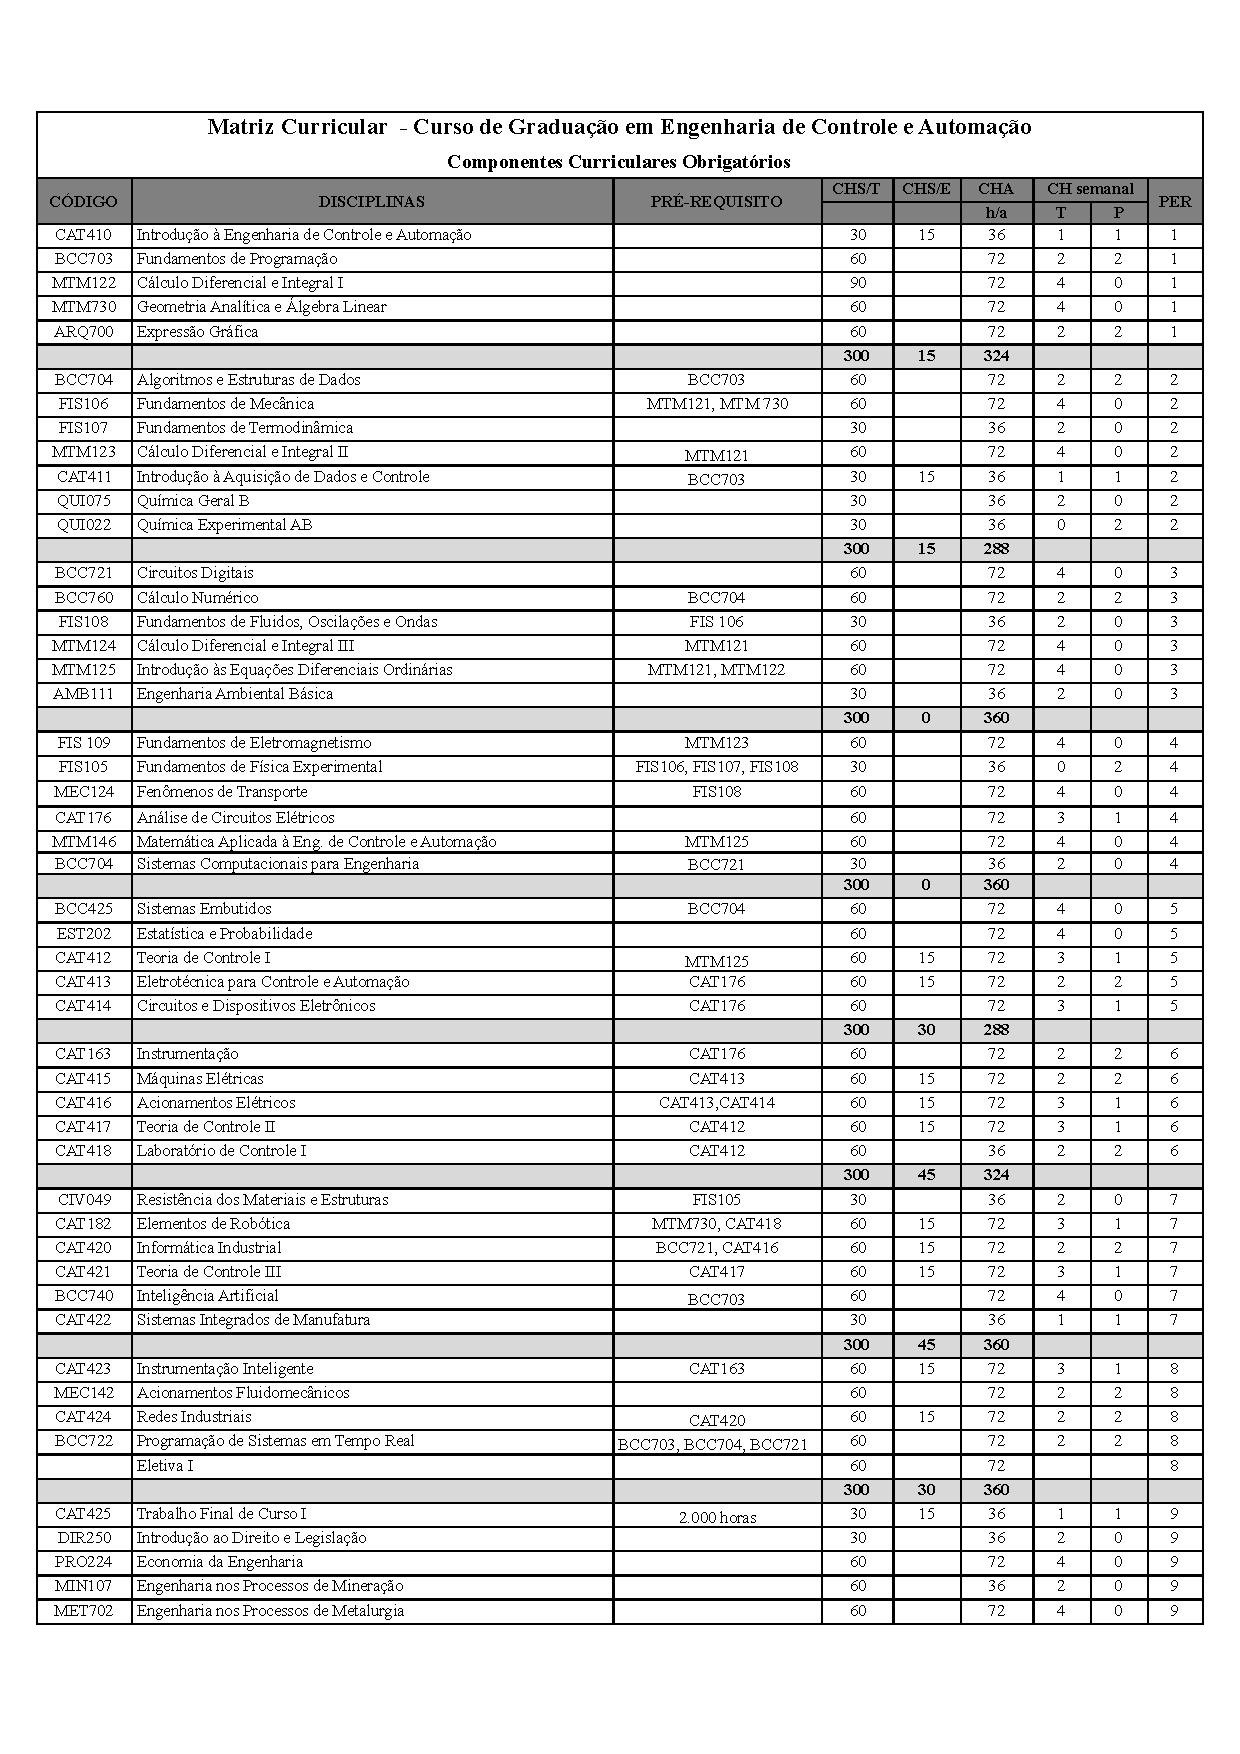
\includepdf[pages=-,nup=1x1,frame]{obrigatorias}


\subsection{Componentes Curriculares Eletivos }\label{tab:0403}

Nesta seção~(\ref{tab:0403}) são apresentadas as disciplinas eletivas. As áreas no quadro de disciplinas eletivas são organizadas por um agrupamento entre os diversos departamentos.

%%%% TABELA DE ELETIVAS {ARQUIVO eletivas.pdf}
 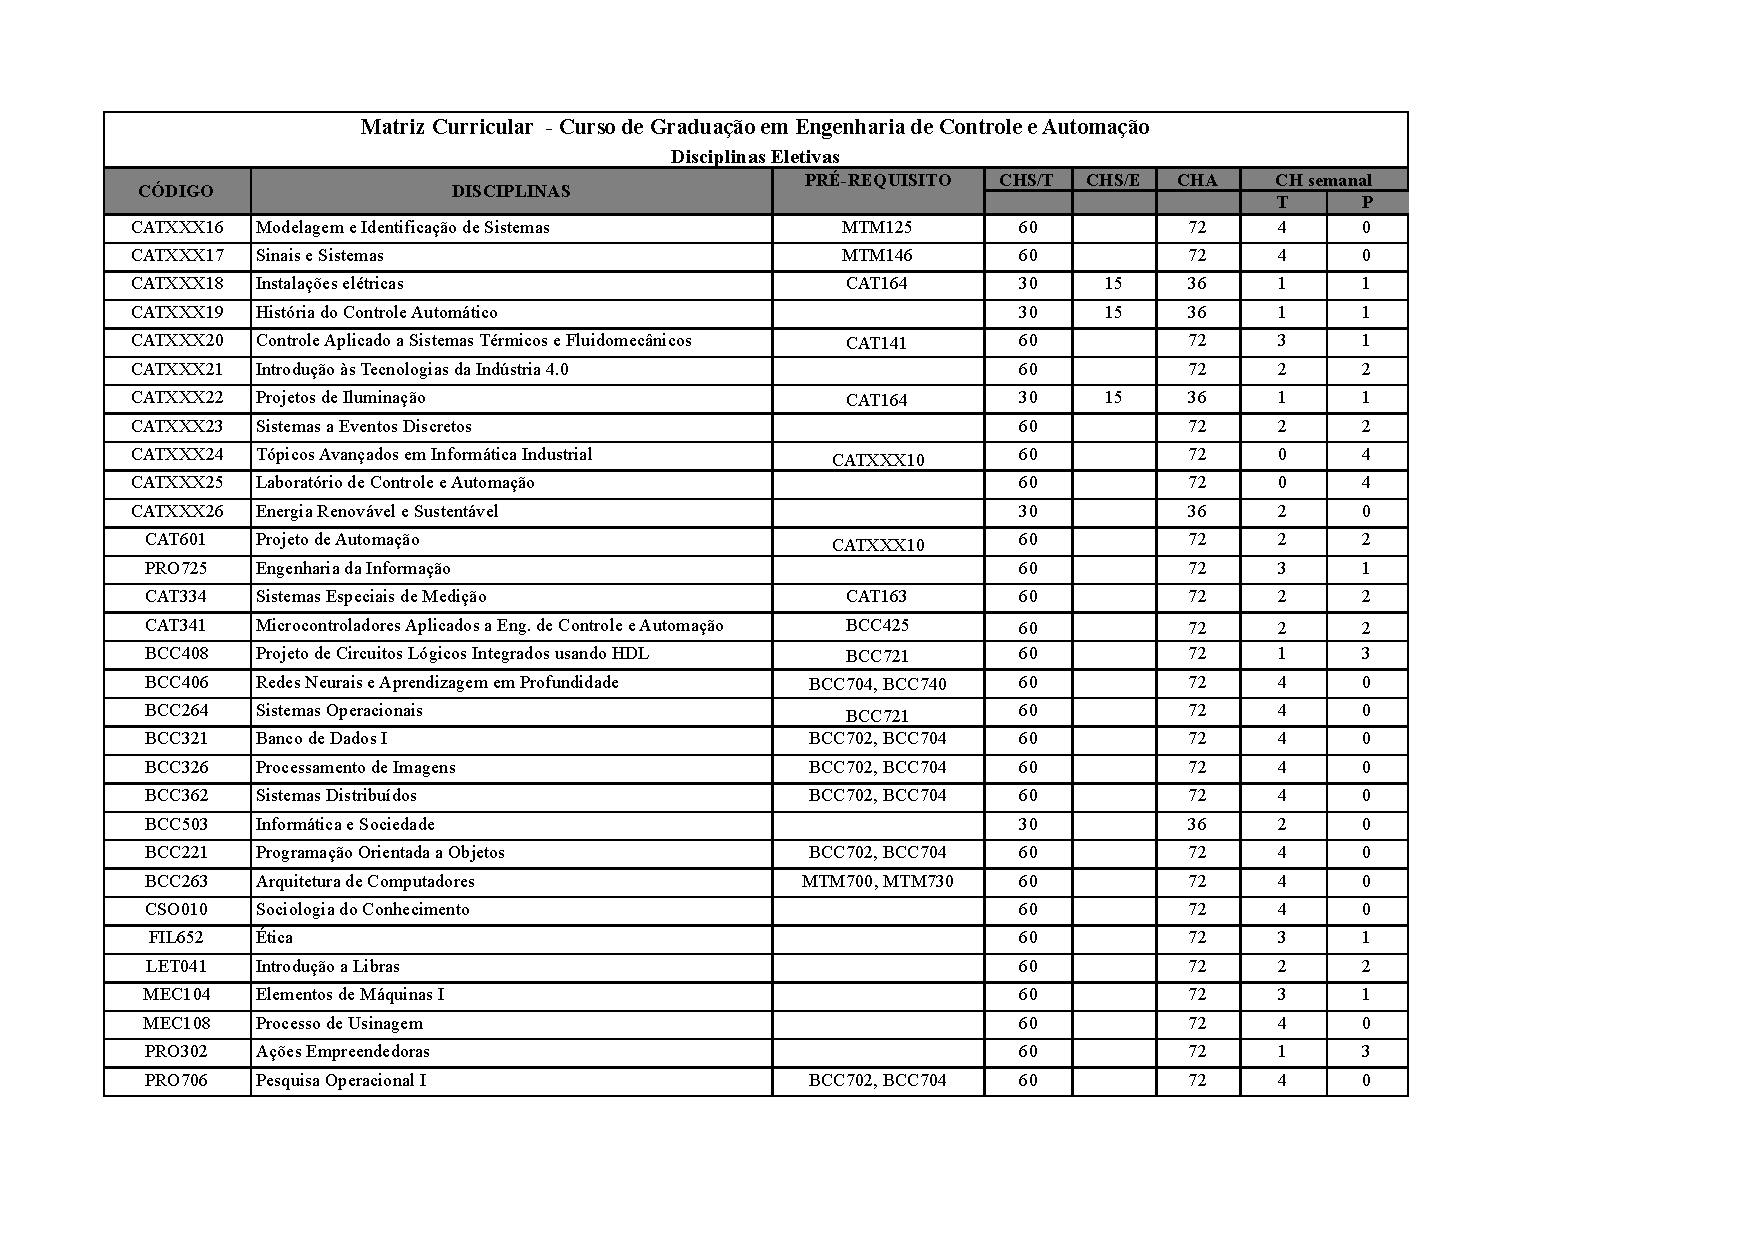
\includepdf[pages=-,nup=1x1,frame]{eletivas}


\section{Proposta curricular}
As disciplinas presentes na Matriz Curricular terão sua carga horária alocada para aulas totalmente teóricas, ou totalmente práticas ou dividida em aulas teóricas e práticas, de acordo com o aprovado no PPC. O professor é livre para avaliar o discente tanto em atividades teóricas quanto práticas da forma que melhor lhe convir.

\section{ENADE}

De acordo com o relatório do Instituto Nacional de Estudos e Pesquisas Educacionais Anísio Teixeira (INEP) acerca do Exame Nacional de Desempenho dos Estudantes (ENADE) realizado em 2014 para o curso de Engenharia de Controle e Automação da UFOP (último realizado antes da elaboração deste PPC), o curso obteve conceito 4 numa avaliação de 1 a 5.  A prova foi composta por 40 (quarenta) questões sendo 30 (trinta) de Conhecimento Específico e 10 (dez) questões de Formação Geral.

De acordo com o relatório, a média do desempenho dos (as) discentes (as) da UFOP no curso de Engenharia de Controle e Automação ficou acima da média do Estado de Minas Gerais e também a do Brasil tanto no Componente de Formação Geral quanto no de Conhecimento Específico.

Observou-se que os discentes tiveram menor dificuldade nas questões de Formação Geral obtendo melhor nota nesse Componente da prova. Como exemplo, na avaliação de 0 a 100, 45,5\% dos discentes do curso de Engenharia de Controle e Automação da UFOP obtiveram nota entre 70 e 80 contra 21,6\% para o total para nota Nacional e 18,2\% obtiveram nota entre 80 e 90 pontos contra 11,5\% para a nota Nacional.

Nas questões de Conhecimento Específico observou-se que a maior parte dos discentes tiveram mais dificuldade sendo que 54,5\% dos discentes ficaram com a nota entre 40 e 60 pontos. Esse resultado ainda está acima da maioria Nacional em que 49,4\% das notas se concentraram entre 20 e 40 pontos.

Mesmo com o conceito 4 obtido, o ENADE/2014 aponta que há a necessidade de melhorias no curso, principalmente no que diz respeito aos conhecimentos específicos da área de controle e automação. Os professores e técnicos administrativos trabalham ativamente buscando essa melhoria e a melhora do conceito obtido pelos discentes do curso no ENADE/2014 (considerando o conceito 3 anterior à avaliação de 2014) é prova desse esforço contínuo.

\section{Programas de disciplinas}
No anexo \ref{ape:01} estão disponíveis os programas das disciplinas obrigatórias para o discente do curso de Engenharia de Controle e Automação contendo a ementa da disciplina, o seu conteúdo programático e sua bibliografia.

\section{Trabalho de conclusão de curso}
O Trabalho de Conclusão de Curso (TCC) ou Monografia é um componente curricular obrigatório para a formação do (a) Engenheiro (a) de Controle e Automação da Universidade Federal de Ouro Preto.

O TCC é a demonstração, por parte do discente, de domínio dos conhecimentos fundamentais da área de conhecimento correspondente. Ele deve constituir de um projeto na área da Engenharia de Controle e Automação, executado pelo discente individualmente sob a orientação de um professor e podendo, opcionalmente, ser coorientado por outro docente. Todo o trabalho deve ser documentado e submetido à avaliação de uma banca examinadora.

A defesa é aberta ao público e constitui-se na apresentação oral do trabalho pelo discente para a banca com duração de 20+/-5minutos, seguida de uma arguição pelos membros da banca. Qualquer recurso didático pode ser utilizado para a apresentação desde que o recurso esteja disponível e se respeite o espaço e o tempo limite da apresentação. Após a defesa a banca se reunirá para deliberar sobre a aprovação da monografia do discente sendo o resultado informado ao discente no mesmo dia da defesa.

As regras para a elaboração da Monografia, definindo os procedimentos e a organização do relatório, foi elaborada pelo Colegiado do Curso de Engenharia de Controle e Automação (CECAU) e se encontra na Resolução CECAU 003/2022 (ver anexo \ref{resolucoes-cecau}). Toda monografia do curso de Engenharia de Controle e Automação deve ter uma cópia da sua versão final disponível na biblioteca da Escola de Minas na UFOP. Casos especiais acerca da Monografia não englobados nesse item, devem ser tratados junto ao CECAU via requerimento.
%

\section[Atividades Complementares]{Atividades Complementares, Estágio e Trabalho de Conclusão de Curso}

As atividades complementares englobam as atividades acadêmicas desenvolvidas pelos discentes ligadas a programas de pesquisa, projetos integradores, monitoria, visitas técnicas, participação em eventos acadêmicos, cursos de curta ou longa duração e extensão da UFOP. Essas atividades complementares, para o estudante de Engenharia de Controle e Automação da UFOP, são regidas por normas específicas da UFOP, recebendo a concessão de créditos/horas conforme Resolução CEPE $n^{\circ} 1.987$ e obedecendo critérios estabelecidos pelo Colegiado do Curso.

\subsection{Atividades Acadêmico Científico-Culturais (AACC)}
Parte das atividades complementares são organizadas em Atividades Acadêmico-Científico-Cultural (AACC) e Atividades Acadêmico-Científico-Cultural Extensionistas (AACCE). Nas Resoluções CECAU 01/2022 e 02/2022, presente nos anexos deste PPC, é possível encontrar as tabelas com as horas aproveitáveis para AACCE e AACC, respectivamente, de acordo com as atividades realizadas pelo discente bem como a regulamentação para a concessão dessas horas. Tais atividades constituem uma excelente forma de incentivar o discente a articular teoria e prática utilizando-se de conhecimentos multidisciplinares, e devem ser desenvolvidas, preferencialmente, em uma área da Engenharia de Controle e Automação e são incentivadas pelo Docente Orientador Acadêmico.

Atividades complementares de monitoria, mini cursos e pesquisa podem ser aproveitadas como AACC e constituem uma excelente forma de incentivar o discente a articular teoria e prática utilizando-se de conhecimentos multidisciplinares. Estudantes veteranos que auxiliarem no acolhimento/orientação de calouros também podem aproveitar tal tarefa como AACC.

O aproveitamento de horas para AACC e AACCE devem ser solicitados na Seção de Ensino da Unidade Acadêmica em que o curso se encontra alocado, de acordo com as resoluções CECAU 01/2022 e 02/2022 (ver anexo \ref{resolucoes-cecau}). Para o curso de Engenharia de Controle e Automação essa unidade é a Escola de Minas. A Seção de Ensino encaminhará o pedido de aproveitamento ao Colegiado do Curso de Engenharia de Controle e Automação para avaliação.

\subsection{Estágio curricular supervisionado}
O estágio supervisionado é componente curricular obrigatório no curso de Engenharia de Controle e Automação da UFOP e é mais uma oportunidade do discente aplicar na prática os conhecimentos adquiridos na Universidade e de também trazer para a Universidade os conhecimentos daquilo que é tendência e necessidade nas empresas, aprofundando seus estudos numa determinada área de interesse, no restante do curso, além de contribuir para a melhoria contínua do deste. De acordo com o § 2o do Art. 11 das Diretrizes Curriculares Nacionais para os Cursos de Engenharia.

        § 2o No âmbito do estágio curricular obrigatório, a IES deve estabelecer parceria com as organizações que desenvolvam ou apliquem atividades de Engenharia, de modo que docentes e discentes do curso, bem como os profissionais dessas organizações, se envolvam efetivamente
        em situações reais que contemplem o universo da Engenharia, tanto no ambiente profissional quanto no ambiente do curso.

A realização do estágio é possível após a integralização de 1500 horas do curso de Engenharia de Controle e Automação. O total de horas do estágio deverá ser de, no mínimo 160 (cento e sessenta) horas, sendo permitido mais de um estágio a fim de completar a carga horária obrigatória.  Com isso, o estudante de Engenharia de Controle e Automação da UFOP terá a oportunidade de aplicar os conhecimentos adquiridos no curso além de ter uma melhor ideia das disciplinas eletivas que gostará de cursar para aprofundar seus estudos numa determinada área.

O discente terá o acompanhamento de um professor e após a conclusão e aprovação da atividade o discente irá obter os créditos correspondentes. As diretrizes e normas correspondentes foram elaboradas pelo Colegiado do Curso de Engenharia de Controle e Automação, em conformidade com as resoluções que tratam do assunto, entre elas as Resoluções CEPE 2.088, CEPE 1.586, CEPE 1.681, CUNI 1868, CEPE 4450 e CEPE 450 e se encontra na Resolução CECAU 04/2022 (ver anexo \ref{resolucoes-cecau}).

\subsection{Trabalho de Conclusão de Curso}
No último ano o discente de Engenharia de Controle e Automação da UFOP deverá matricular-se nas disciplinas Trabalho Final de Curso I e II e, sob a orientação de um professor, desenvolve um trabalho, na área para a qual fez opção para aprofundar seus estudos, o que dará origem à monografia que será defendida perante comissão examinadora, no final do décimo período, como requisito para obter o grau de Engenheiro(a) de Controle e Automação.

\section{Organograma do Curso}
%
A estrutura organizacional da UFOP está descrita em seu estatuto (Resolução CUNI nº 1868, de 17 de fevereiro de 2017). De acordo com o Estatuto da UFOP, a organização dos órgãos superiores de deliberação é composta pelos: Conselho Universitário (CUNI) que é assessorado pela Câmara de Pessoas, Câmara de Infraestrutura e pela Câmara de Orçamento e Finanças; Conselhos superiores compostos pelo Conselho Superior de Graduação, Conselho Superior de Pesquisa e Pós-Graduação e pelo Conselho Superior de Extensão e Cultura; Conselho de Curador (CONC), Reitoria, Unidades Acadêmicas, Conselhos das Unidades, Colegiados de Cursos e Departamentos.

O curso de Engenharia de Controle e Automação está alocado na Unidade Acadêmica da Escola de Minas e está sob as decisões do Conselho Deliberativo da Escola de Minas (CDEM). O Colegiado do Curso de Engenharia de Controle e Automação (CECAU) é a instância universitária responsável pela coordenação didática das disciplinas constituintes do projeto pedagógico do curso.

De acordo com o Regimento da UFOP,\footcite{resolucao-cuni-1959} em seu Art.170:
\begin{quotation}
“O corpo discente terá representação, com direito a voz e a voto, nos órgãos colegiados da Universidade e das unidades acadêmicas, na forma do Estatuto e deste Regimento”.
\end{quotation}

O discente terá o mandato de um ano, permitida uma recondução, independentemente do cumprimento integral ou não do mandato anterior.

Os estudantes do curso de Engenharia de Controle e Automação integram o Centro Acadêmico da Engenharia de Controle e Automação (CAECA). A entidade é a representante dos(as) discentes, representando-os(as) na Assembleia Departamental, bem como no Colegiado de Curso. Além de eleger os representantes discentes para os órgãos colegiados, o CAECA também realiza a integração dos(as) discentes do curso de Engenharia de Controle e Automação da UFOP e amplia o conhecimento dos(as) estudantes por meio da promoção de eventos, tais como a Semana de Estudos da Escola de Minas, visitas técnicas e palestras complementares, organização de cursos de formação complementar, integrações festivas, bem como a divulgação de cursos e oportunidades de interesse no campo de controle e automação.

Em relação as Unidades Administrativas, a responsabilidade máxima é exercida pelo(a) Reitor(a) (competindo ao(a) Vice-Reitor(a) colaborar com ele(a) nas funções a ele(a) delegadas e substituí-lo(a) nos casos de falta, impedimento ou de vacância) e é gerida pela Reitoria (além da Vice-Reitoria), pelas Pró-Reitorias e pelos setores a esses subordinados (PDI UFOP, 2016). Nesse âmbito, a Pró-Reitoria de Graduação (PROGRAD) é a responsável para ``proposição, coordenação e acompanhamento da política de graduação da UFOP. É também a instância encarregada dos processos seletivos e do gerenciamento acadêmico dos cursos de graduação''\footcite{PDI-UFOP}. Assim, o organograma do curso de Engenharia de Controle e Automação se organiza conforme a Figura \ref{fig:organograma}.

\begin{figure}[hbtp]
	\centering
	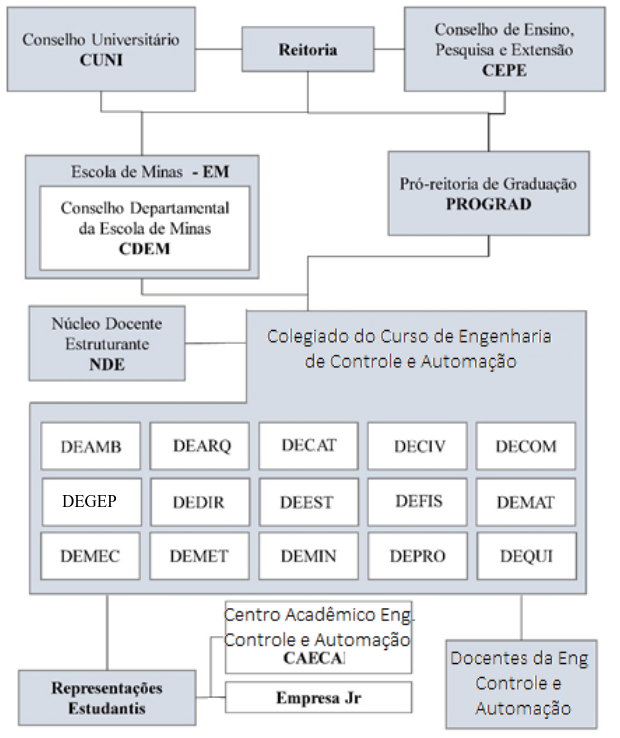
\includegraphics[scale=0.7]{estrutura-administrativa}
	\caption{Organograma do curso de Engenharia de Controle e Automação.}
	\label{fig:organograma}
\end{figure}


\section{Flexibilização Curricular}
O currículo do curso de Engenharia de Controle e Automação da UFOP é composto por disciplinas de diversos departamentos da UFOP, o que possibilita a formação interdisciplinar ao discente. Nas tabelas \ref{tab:0402} e \ref{tab:0403} estão disponíveis disciplinas obrigatórias e eletivas de diversos cursos da Universidade Federal de Ouro Preto. A qualquer momento do curso, o discente de Engenharia de Controle e Automação pode cursar disciplinas de outros departamentos (obedecendo-se os pré-requisitos destas), mesmo que estas não constem na grade curricular, ou realizar atividades acadêmicas extracurriculares. O discente pode requerer a contabilização dos créditos destas de acordo com as resoluções CEPE  Nº  1.586 e CEPE  Nº  1.681.

\section{Relação com a Pesquisa}

A pesquisa no curso de Engenharia de Controle e Automação é estruturada em diversas frentes, de modo a permitir ampla participação do discente.

Além dos programas de Iniciação Científica já tradicionais e executados no âmbito da PROPPI e do TCC relatado sob a forma de trabalho científico (monografia ou artigo), o Departamento de Engenharia de Controle e Automação desenvolve outras modalidades de incentivo à Pesquisa:

\begin{itemize}
    \item Compondo a equipe dos professores em projetos em projetos de pesquisa da FAPEMIG e do CNPq.
    \item Em apoio aos pós-graduandos em atividades de laboratório e campo.
    \item Participando de palestras, seminários e outras atividades propostas pela Coordenação da Pós-Graduação.
\end{itemize}

Para além das iniciativas mencionadas, vale ressaltar que discentes do curso são envolvidos, no decorrer da formação acadêmica, em pesquisas integrantes de disciplinas que compõem o currículo e incentivados à escrita de resumos e artigos científicos. Todas estas ações são passíveis de pontuação em AACCE, conforme a tabela das AACCEs presente na Resolução CECAU 01/2022 nos anexos a este PPC.


\chapter{Curricularização da Extensão}

\section{Integração entre Ensino, Pesquisa e Extensão}

O discente do curso de Engenharia de Controle e Automação da UFOP dispõe de diversas possibilidades para complementar sua formação em atividades multidisciplinares que podem também integrar diferentes cursos da UFOP e a própria sociedade. A política aqui se insere no âmbito da política institucional de formação para os cursos de Engenharia, conforme a resolução CUNI Nº 2544, de 2022.\footcites[Em especial podemos citar o trecho II da referida política, que inclui os chamados Núcleos e Estruturas de formação, bem como a questão da curricularização da extensão. Ver em][pp.~16--26]{politica-eng-2022-ufop}\footnote{Alguns outros itens foram também inspirados no Projeto Político e Pedagógico do Curso de Administração da UFOP, disponível no sistema SEI sob o número $23109.006535/2022-03$, de 23 de maio de 2022.}

Conforme explicitado pela Política Institucional de formação para os cursos de Engenharia da UFOP, firmado ao longo das reuniões da subcâmara de graduação e das políticas de engenharia, no início do ano de 2022, levando-se em consideração uma das características marcantes dos cursos de engenharia da UFOP como o seu forte embasamento teórico, ``...~os núcleos e estruturas de formação são pensados de maneira a promover uma formação generalista, promovendo forte integração entre o ciclo básico e o profissionalizante, aliada à uma formação cidadã e ética'',\footcite[p.~17]{politica-eng-2022-ufop} espera-se que o processo de formação profissional esteja assentado em 5 eixos básicos, que visem promover, resumidamente:
\begin{enumerate}
    \item Uma formação ética que compreenda o papel social da engenharia e no uso de tecnologias em prol da sociedade;
    \item Uma formação homogênea e inclusiva;
    \item A Criação de conhecimentos relacionados a filosofia, sociologia, história e à cultura;
    \item O conhecimento sólido em matemática, física, química, estatística e computação;
    \item Relações com o mundo do trabalho que contribuam para o processo de aprendizagem.
\end{enumerate}

No contexto do ensino, das atividades didáticas e dos itens que devem ser incluídos nos currículos, deve-se ressaltar a importância de ações que visem o desenvolvimento de habilidades de cada indivíduo, cada estudante, e que podem ser divididas nas chamadas \textit{soft skills} -- que são habilidades eminentemente comportamentais como ética, responsabilidade, compromisso, comunicação e escrita, expressão, entre outras -- e as \textit{hard skills} -- que englobam o saber técnico \emph{per se}, tais como conhecimentos em matemática, física, computação e demais elementos técnicos inerentes à cada área do conhecimento. Levando-se ainda em consideração a notória preferência dada ao saber puramente técnico e tecnológico dentro dos diversos campi das universidades brasileiras, faz-se necessário identificar deficiências existentes no contexto do curso de Engenharia de Controle e Automação, bem como propor soluções no intuito de promover um melhor balanço no estímulo das habilidades essenciais para uma boa formação.

Além disso, no que tange ao curso de Engenharia de Controle e Automação, a busca por esse balanço passa, necessariamente, pelas atividades de extensão, considerando-se o processo de implantação da curricularização que as IFES estão vivenciando. A lei 13.005 de 25 de junho de 2014 previa que, até 2024, as universidades brasileiras deveriam possuir no mínimo 10\% da carga horária de seus cursos voltada e contabilizada como extensão. Isso significa que o estudante de graduação deverá participar de ações de extensão onde o público-alvo prioritário deverá ser a comunidade externa à universidade. Mais especificamente, no âmbito das atividades do curso de Graduação em Engenharia de Controle e Automação, tais ações impactarão em um total de 360 horas que deverão ser desenvolvidas em atividades de extensão, como programas, projetos, ações isoladas ou nas chamadas disciplinas de caráter extensionista.

As ações de extensão universitária, de forma indissociável ao ensino e à pesquisa, promovem interações transformadoras entre a universidade e outros segmentos da sociedade, através de um processo interdisciplinar, educativo, cultural, científico e político, que promove intervenções diretas com as comunidades externas. \footcite{guia-curricularizacao-2022} Neste sentido, uma ação de extensão deve, obrigatoriamente, envolver estudantes e setores da sociedade, sempre sob a coordenação de um docente ou de um técnico administrativo, e promover interações entre as demandas da sociedade e os saberes gerados no âmbito da universidade.


\section{Programas e Projetos de Extensão}
As ações de extensão propiciam a estudantes da UFOP a formação de novos conhecimentos e habilidades transversais, desenvolvendo, simultaneamente, habilidades técnicas e sociais de forma intuitiva. Em consonância com os objetivos da Política Nacional de Extensão Universitária,\footcite{forproex2012} que embasaram a criação da Resolução CEPE 7.609, de 2018,\footcite[][]{resolucao-cepe-7609} as atividades de extensão no âmbito do DECAT se voltam a afirmar a extensão universitária como processo acadêmico definido em função das exigências da realidade, além de ser importante elemento na formação do estudante, na qualificação da(o) docente e no intercâmbio com a sociedade. Tais contribuições são fundamentadas em uma forma específica de se produzir conhecimento, tendo como fundamento o  diálogo e a troca de experiências e saberes, em sincronia com os anseios da sociedade, aliando movimentos, organizações e setores da sociedade civil.

Um elemento relevante da política de extensão incluída neste PPC é a busca pelo aprimoramento de uma formação humanista do discente e na produção de conhecimento. Para isso, foi ponderado que ações multidimensionais deveriam ter um caráter primordial, considerando-se que elas possuem, por si mesmas, grande importância na relação entre universidade e sociedade. Neste sentido, a curricularização de atividades de extensão na área de Engenharia de Controle e Automação -- fundamentada na política nacional de extensão universitária -- se fundamenta na ``...~Interação Dialógica, Interdisciplinaridade e Interprofissionalidade, Indissociabilidade Ensino-Pesquisa-Extensão, Impacto na Formação do Estudante, e Impacto e Transformação Social''.\footcites[][p.~29]{forproex2012}[Ver também a própria politica das engenharias da UFOP, conforme a resolução CEPE/UFOP 7609/2018, em][]{politica-eng-2022-ufop} Dessa forma, as ações de extensão ficam assim caracterizadas:

\begin{itemize}
\item \textbf{Ações Institucionais:} são aquelas elaboradas para atender a demandas externas à UFOP advindas de órgãos e instituições federais, estaduais ou municipais, ou aquelas elaboradas para atender a demanda de interesse da Administração Superior.
\item \textbf{Prestação de serviços:} refere-se ao estudo e à solução de problemas do meio profissional ou social, com a participação orientada de estudantes, e ao desenvolvimento de novas abordagens pedagógicas e de pesquisa, bem como a transferência de conhecimentos e tecnologia à sociedade. Neste âmbito podem se inserir iniciativas de produção de materiais didáticos e paradidáticos na forma escrita em meio físico e digital, tais como artigos para enciclopédias online e até conteúdo audiovisual para plataformas de \textit{streaming}.
\item \textbf{Evento:} ação que implica na apresentação e/ou exibição pública, livre ou com clientela específica, do conhecimento ou produto cultural, artístico, esportivo, científico e tecnológico desenvolvido, conservado ou reconhecido pela Universidade e que atenda as diretrizes dispostas na Resolução CEPE citada. Os eventos de extensão podem ser:
\begin{itemize}
    \item \textit{Congresso:} evento de grandes proporções, de âmbito regional, nacional ou internacional, em geral com duração de 3 a 7 dias, que reúne participantes de uma comunidade científica ou profissional ampla. Abrange um conjunto de atividades tais como mesas-redondas, palestras, conferências, oficinas, \textit{workshops} e minicursos, estes com duração de até 8 (oito) horas.
    \item \textit{Seminário:} evento científico de âmbito menor do que o congresso, tanto em termos de duração (horas a 1 ou 2 dias), quanto em número de participantes, cobrindo campos de conhecimento mais especializados. Incluem-se nessa classificação encontros, simpósios, jornadas, palestras, colóquios e fóruns.
    \item{Ciclo de Debates:} encontros sequenciais que visam à discussão de um tema específico, podendo ser caracterizados como Ciclos, Circuitos, Semanas ou similares.
    \item \textit{Exposição:} exibição pública, podendo incluir Feiras, Salões, Mostras, Lançamentos ou similares.
    \item \textit{Espetáculo:} demonstração pública de eventos cênicos ou musicais, incluindo recital, concerto, show, apresentação teatral, exibição de cinema e televisão, demonstração pública de canto, dança e interpretação musical.
    \item \textit{Evento esportivo:} campeonato, torneio, olimpíada ou apresentação esportiva.
    \item \textit{Festival:} série de ações/eventos ou espetáculos artísticos, culturais ou esportivos, realizados concomitantemente, em geral com edições periódicas.
    \item \textit{Outros:} ação pontual de mobilização que visa um objetivo definido.
\end{itemize}
\item \textbf{Ações usuais:} são aquelas submetidas por proponentes da UFOP, podendo ser enquadradas nas seguintes modalidades:
\begin{itemize}
    \item \textbf{Programa:} conjunto articulado de ações ou projetos de extensão, integrando-as à pesquisa e ao ensino. Tem caráter mais abrangente, com clareza de diretrizes e orientação para um objetivo comum a ser executado em médio e longo prazos. Normalmente atende uma mesma comunidade. O prazo mínimo de execução do programa deve ser de dois anos.
    \item \textbf{Projeto:} ação processual e contínua de caráter educativo, social, cultural, científico ou tecnológico, com objetivo específico e prazo determinado. Este, por sua vez, pode ser isolado ou vinculado a um programa de extensão.
    \item \textbf{Curso:} ação pedagógica, de caráter teórico e/ou prático, presencial ou à distância, planejada e organizada de modo sistemático, com prazo determinado e carga horária mínima de 8 (oito) horas e critérios de avaliação definidos. Ações dessa natureza com menos de 8 (oito) horas devem ser classificadas como ``evento''. %É obrigatório o envolvimento de discentes de graduação em todas as ações de Extensão, além de servidor(es) docente(s) ou técnico-administrativo(s).
\end{itemize}
\end{itemize}


As atividades de ensino, especificamente na forma de exposição oral, poderão ser exercidas em todas as disciplinas, no tempo mínimo de 30 (trinta) minutos, podendo o docente praticar, nas horas restantes, atividades outras, com todas as variações metodológicas possíveis, com a prévia aprovação do plano de ensino pelo Colegiado do Curso. Nessa mesma perspectiva, o PDI-UFOP pondera que se deve buscar que o ensino se integre ao conhecimento produzido pela pesquisa e se realize, sempre que possível, por meio da atividade de pesquisa.\footcite[p.~34]{PDI-UFOP} Ao mesmo tempo, deve-se buscar, em conjunto com a atividade de pesquisa, articular o ensino com os anseios gerais da sociedade por meio da realização das atividades de extensão.

Atividades de Extensão Universitária são uma excelente oportunidade para o discente colocar em prática seus conhecimentos acadêmicos em prol da sociedade bem como pesquisar e/ou desenvolver soluções. Nesse tipo de atividade o discente entra em contato com pessoas e problemas que possibilitam uma experiência muito próxima do real mercado de trabalho. Em contrapartida, a sociedade ganha com um serviço prestado. Toda a atividade é coordenada por um  docente que orienta o discente, buscando garantir a correta execução do projeto junto à sociedade. Atividades de extensão podem envolver discentes de diferentes cursos da Universidade.

Uma das metas principais dessa integração é, justamente, fortalecer os projetos de curricularização dos diferentes cursos da Escola de Minas, incentivando projetos com grande potencial de participação ativa de graduandos e grande impacto na sociedade. Além disso, pretende-se garantir as condições de infraestrutura para a realização de diferentes ações de extensão vinculadas às propostas de curricularização da extensão nos vários cursos da Escola de Minas da UFOP, não apenas o curso de Engenharia de Controle e Automação.

Equipes multidisciplinares também podem ser formadas para a realização de projetos independentes voltados para a participação em competições de estudantes, por exemplo. Neste aspecto a(o)s estudantes podem ter contato com equipes de outras instituições, em busca de um resultado comum, que incentiva o aprendizado e a pesquisa. Tais projetos são também orientados por docentes que coordenam as atividades desempenhadas por cada estudante, bem como o uso dos recursos financeiros.\footnote{No site do DECAT é possível conhecer mais detalhes sobre as equipes de competição compostas por discentes do curso. Ver em~\url{https://decat.ufop.br}.}


Outra possibilidade que o(a) discente de Engenharia de Controle e Automação da UFOP tem de colocar em prática seus conhecimentos acadêmicos é por meio das Empresas juniores, que possibilitam ao discente uma oportunidade de empreender e ter uma experiência mais próxima do mercado de trabalho. A pesquisa é incentivada pelos projetos da empresa e tudo é acompanhado por um docente. Neste aspecto, o Centro de Referência em Incubação de Empresas e Projetos de Ouro Preto (Incultec) pode, inclusive, oferecer a oportunidade para o discente transformar sua ideia em produto ou negócio. Ao incentivar o empreendedorismo, a Incultec pode transformar um bom projeto de pesquisa algo maior.

\section{Operacionalização das ações de extensão universitária}
%
Não é desproposital afirmar que a universidade pública deve, em última instância, buscar a otimização dos recursos públicos em atividades que tenham como fim a natureza pública e gratuita, em prol da sociedade como um todo, começando-se, naturalmente, pelo entorno físico dos diversos campi da UFOP, mas não necessariamente limitados a estes. É preciso buscar estes espaços, em que os discentes e docentes do curso de Engenharia de Controle e Automação, de alma eminentemente tecnológica, possam se inserir.

Se a questão da interdisciplinaridade e da transdisciplinaridade criam desafios incontornáveis na concepção e elaboração dos cursos de graduação, muitos deles vinculados a tradições disciplinares previamente estabelecidas, em sua maioria, por meio da diferenciação entre os setores do conhecimento e competências de cada setor, na extensão universitária as possibilidades de interfaceamento ou de contato são incontáveis. No entanto, para a sua operacionalização, é de fundamental importância a existência de espaços de trabalho em conjunto, espaços que permitam o diálogo e a elaboração de propostas que atravessem, partindo-se dos eixos comuns já citados,\footcite[Ver, por exemplo, o capítulo 3 da política de formação para os cursos de engenharia, em que tais eixos são justamente especificados. ver em][p.~13]{politica-eng-2022-ufop} as ``fronteiras da universidade'', mencionadas anteriormente.\footcite[Ver também][]{varellaetal2022}

A operacionalização da extensão no curso de Engenharia de Controle e Automação da UFOP tem por objetivo permitir que o discente participe de Ações de Extensão Universitária como um processo dialógico de produção de conhecimento e instrumento de desenvolvimento sócio-político-cultural. As ações serão efetivadas por meio de: Programas, Projetos, Cursos, Eventos e Disciplinas.

Baseado no exposto acima e, a fim de proporcionar condições aos discentes do curso de Engenharia de Controle e Automação da UFOP a integralização da carga horária de 330 horas referente aos 10\% da carga horária do curso, este Projeto Pedagógico prevê horas de extensão em disciplinas obrigatórias e eletivas do curso, Atividades Acadêmicas Científicas e Culturais Extensionistas (ver tabela presente na Resolução CECAU XXX nos anexos a este PPC) -- em conformidade com o guia de curricularização da extensão, veiculado pela PROEX, a Pró-Reitoria de Extensão e Cultura da UFOP, em março de 2022,\footcite[Ver em][]{guia-curricularizacao-2022} além de estágios não obrigatórios, por meio da Resolução CONEC/UFOP Nº19/2022,\footcite{CONEC-UFOP-19-2022} em que foram definidas normas e critérios para a utilização da carga horária de estágios não obrigatórios para a curricularização da Extensão Universitária na UFOP. A essência desse conjunto de ações pode ser especificada por meio dos detalhes de cada eixo.

São articuladas 13 disciplinas obrigatórias parcialmente extensionistas, distribuídas do primeiro ao nono período do curso, além de três disciplinas eletivas, as quais terão parte da sua carga horária com caráter extensionista, conforme elucidado no tópico seguinte. A diluição da carga horária em diferentes disciplinas ao longo do curso tem por objetivo possibilitar que mais docentes participem de atividades extensionistas. Além disso, será possível realizar projetos que envolvam educação/ações continuadas de acordo com os temas que os discentes do curso de Engenharia de Controle e Automação estarão cursando. A inserção da sociedade, seja alcançando as escolas de educação básica ou a comunidade próxima aos campi da UFOP, em temas do cenário atual e cada vez mais agressivo e presente no nosso dia a dia, relacionados a inserção no mundo digital, da inteligência artificial, da robótica e até de assuntos mais corriqueiros como lidar com a energia elétrica e seus riscos/benefícios, que estão inseridos no cotidiano da sociedade, mas que em sua grande maioria não são efetivamente compreendidos por ela.


\section{Disciplinas Extensionistas}
Algumas das disciplinas que, no seu escopo, têm ações extensionistas, estão distribuídas ao longo do curso. Essa organização possibilita que a(o) discente tenha contato e desenvolva ações extensionistas por meio das disciplinas durante grande parte da vida acadêmica.

Cabe explicitar que se tratam, em sua maioria, de disciplinas obrigatórias do curso, o que garante um amplo acesso à extensão por discentes do curso de Engenharia de Controle e Automação. Pode-se observar na lista em seguida a descrição de cada disciplina extensionista oferecida, com as ações especificadas. Para consultar a carga horária de cada disciplina destinada às ações extensionistas, além do seu caráter eletivo ou obrigatório inseridos na matriz curricular, consultar o anexo~\ref{ape:01}, em que os programas de cada disciplinas são apresentados. As disciplinas que possuem caráter extensionista são descritas a seguir:

\begin{itemize}
    \item \textbf{CAT410 -- Introdução à Engenharia de Controle e Automação:} Os estudantes serão apresentados à Engenharia de Controle e Automação nessa disciplina, na estrutura da graduação e nas áreas de atuação do profissional. Como atividade extensionista, os estudantes, a partir de uma análise crítica do que foi discutido na disciplina, e em parceria com escolas da educação básica, irão promover rodas de conversa sobre o papel da automação na sociedade atual, buscando promover um processo de reflexão acerca dos impactos sociais da automação, além de estimular a inserção de novos talentos nas carreiras tecnológicas.

    \item \textbf{CAT411 -- Introdução à Aquisição de Dados e Controle:} Introdução à Aquisição de Dados e Controle: Nessa disciplina, o discente será apresentado a alguns componentes básicos de eletrônica, tais como: chaves, botões, resistores, LEDs, fontes de alimentação, entre outros, e deverá, ao final do curso, ser capaz de montar pequenos projetos envolvendo os componentes estudados. Após isso, como atividade extensionista, os estudantes, em conjunto com escolas de educação básica, realizarão atividades em laboratório ou nas escolas da comunidade para discutirem a diferença entre dados e informação, de suma importância em um cenário em que tudo é veiculado com muitos dados, mas poucas informações são de fato extraídas da forma correta.

    \item \textbf{CAT412 -- Teoria de Controle I:} Os discentes farão a construção de plantas (sistemas de controle) a partir de material de baixo custo (de preferência recicláveis) e farão os ensaios necessários para o levantamento dos parâmetros necessários para, em seguida realizar sua modelagem matemática. Todo o passo-a-passo desde a construção da estrutura até a obtenção do modelo será registrada por meio de fotos, vídeo e ilustrações. O material produzido, será disponibilizado de forma pública e gratuita para a comunidade por meio de redes sociais ou plataformas de vídeo. Os estudantes dos ensinos médio e técnico de escolas de Ouro Preto e região, serão convidados a assistir às exposições dos projetos desenvolvidos pelos discentes da disciplina onde serão incentivados participar de discussões sobre a importância dos sistemas de controle na indústria e no dia-a-dia das pessoas como em eletrodomésticos e sistemas inteligentes, cada vez mais comuns na vida de todos. Por fim, os estudantes convidados poderão avaliar os projetos, incentivando os discentes da disciplina a se dedicarem ao desenvolvimento e exposição dos sistemas de controle. Para os estudantes do ensino médio, a contribuição dessa disciplina seria a de compartilhar o conhecimento sobre controle de sistemas e inspirá-los a cursar no futuro um curso na área de ciência, tecnologia e engenharia.

    \item \textbf{CAT413 -- Eletrotécnica para Controle e Automação:} Os estudantes, em conjunto com escolas de educação básica, realizarão atividades em laboratório com aplicações de algumas práticas elétricas que poderão ser usadas no dia a dia. Após a prática serão levantadas rodas de conversa para levantar demandas e curiosidades dos participantes.

    \item \textbf{CAT415 -- Máquinas Elétricas:} Os estudantes da disciplina poderão atuar como mentores em visitas guiadas aos laboratórios de eletrotécnica, mostrando a prática de ligações de partida de motores e funcionamento de algumas máquinas elétricas, tanto para o público de escolas técnicas como para profissionais da área de elétrica da comunidade.  Será disponibilizado o momento de uma mesa redonda para discussão de temas abordados durante a atividade.

    \item \textbf{CAT416 -- Acionamentos Elétricos:} Os discentes serão incentivados a identificar uma comunidade ou instituição parceira onde possam aplicar projetos de extensão relacionados ao dimensionamento e reparo de sistemas de acionamento em equipamentos motorizados, como bombas hidráulicas. O tema será de escolha livre, desde que respeite os princípios da extensão universitária e promova a aproximação entre a universidade e a sociedade. Durante a disciplina, os estudantes serão orientados quanto ao conceito de extensão, à importância do vínculo com a comunidade e às etapas de elaboração de projetos e relatórios técnicos, com foco na aplicação prática dos conhecimentos de acionamentos elétricos em demandas reais.

    \item \textbf{CAT417 -- Teoria de Controle II:} Sob a orientação e tutoria do docente, os estudantes farão a construção de plantas a partir de material de baixo custo (de preferência recicláveis) e farão os ensaios para o levantamento dos parâmetros necessários para, em seguida, realizar sua modelagem matemática e identificação. Todo o passo a passo desde a construção da estrutura até a obtenção do modelo será registrada por meio de fotos, vídeo e ilustrações. O material produzido, será disponibilizado de forma pública e gratuita para a comunidade por meio de redes sociais ou plataformas de vídeo. Estudantes do ensino médio e técnico de Ouro Preto e região serão convidados para demonstrações dos projetos de controle digital implementados. As discussões podem abordar a presença e a importância do controle digital em sistemas embarcados, robótica, automação industrial moderna e dispositivos inteligentes. Podem ser explorados exemplos como o controle de temperatura em sistemas digitais, o controle de movimento em pequenos robôs, ou a implementação de filtros digitais simples. Os estudantes convidados serão incentivados a avaliar os projetos, oferecendo um retorno e incentivando os discentes da disciplina de Teoria de Controle II a aprofundarem seus conhecimentos e aprimorarem suas habilidades na área. Para os estudantes do ensino médio, a contribuição dessa disciplina seria a de compartilhar o conhecimento sobre controle de sistemas e inspirá-los a cursar no futuro um curso na área de ciência, tecnologia, engenharia e matemática.

    \item \textbf{CAT421 -- Teoria de Controle III:} Sob a orientação e tutoria do docente, os discentes da disciplina realizarão testes para identificar os parâmetros essenciais de plantas construídas com material reciclado ou de baixo custo, a fim de desenvolver modelos matemáticos e, posteriormente, projetar e implementar controladores para as plantas. Todas as etapas do processo, desde a construção inicial até a implementação do controlador, serão registradas por meio de recursos visuais como fotos, vídeos e ilustrações. O material resultante desse trabalho será disponibilizado gratuitamente ao público por meio de plataformas online, como redes sociais ou sites de vídeos. Adicionalmente, estudantes do ensino médio e técnico da região de Ouro Preto serão convidados para participar de demonstrações dos sistemas de controle criados. Nessas ocasiões, serão promovidas discussões sobre a relevância do controle em diversas áreas, como sistemas embarcados, robótica, automação industrial moderna e dispositivos inteligentes. Serão apresentados exemplos práticos, como o controle de temperatura, de nível, controle de movimento em robôs pequenos e drones. Os estudantes visitantes serão incentivados a avaliar os projetos, oferecendo um retorno aos alunos da disciplina de Teoria de Controle, com o intuito de estimular o aprofundamento de seus conhecimentos e o desenvolvimento de suas habilidades na área. Para os estudantes do ensino médio, essa iniciativa tem como propósito compartilhar o conhecimento sobre controle de sistemas e despertar o interesse por futuras carreiras nas áreas de ciência, tecnologia, engenharia e matemática.

    \item \textbf{CAT182 -- Elementos de Robótica:} Os estudantes, em articulação com escolas de educação básica, desenvolverão atividades práticas em laboratório universitário ou nas próprias escolas da comunidade, utilizando diferentes kits e tecnologias de robótica educacional. A proposta contempla ainda a realização de rodas de conversa e oficinas com professores da educação básica, com o intuito de identificar demandas pedagógicas e fomentar o uso da robótica como instrumento de apoio ao ensino.a

    \item \textbf{CAT420 -- Informática Industrial:} Os estudantes se reunirão com as comunidades locais em rodas de conversa com o tema “A informática a seu favor”. Haverá oficinas sobre melhores práticas do uso da informática no seu negócio, visualizando a aplicação de um sistema de controle e supervisão ao sistema. Os discentes farão um projeto que envolva o uso de Controlador Lógico Programável e Sistemas Supervisórios, aplicando ideias e dúvidas levantadas por essa roda de conversa. Todo material produzido ficará disponível por meio de exposições (virtuais ou presenciais, a depender dos recursos disponíveis) para escolas do ensino médio de Ouro Preto e Região.

    \item \textbf{CAT423 -- Instrumentação Inteligente:} Como a disciplina consta com um módulo de Inteligência Artificial (IA) no contexto dos sensores inferenciais (\textit{soft sensors}), as práticas extensionistas se concentração no oferecimento de um minicurso de IA e suas aplicações para estudantes do ensino médio (por exemplo, para os estudantes do IFMG), no formato online e utilizando ferramentas computacionais livres e de código aberto como Python, Google Colab, entre outras.

    \item \textbf{CAT424 -- Redes Industriais:} As ações extensionistas da disciplina consistem em realizar manutenção em computadores dos laboratórios de ensino das escolas públicas de Ouro Preto e Mariana. O docente fará um levantamento das escolas interessadas em participar do projeto. Os discentes farão um levantamento das necessidades de software e hardware das máquinas. No caso de falhas de hardware, serão repassadas as especificações dos componentes defeituosos para que a escola efetue a compra. O hardware será substituído, assim que chegar, na própria escola pelos discentes. No caso de falhas de software, o software poderá ser reinstalado ou o computador ser formatado. A escola deverá fornecer as licenças de software ou permitir a instalação de softwares livres.

     \item \textbf{CAT425 -- Trabalho Final de Curso I:} A comunidade local e estudantil da região, sobretudo a concluinte do ensino médio e de escolas de ensino técnico, será convidada a participar ativamente das apresentações dos projetos de conclusão de curso, como uma forma de construção conjunta do conhecimento. Uma roda de conversa com a temática ``o que é ciência?'' Tal espaço será uma forma de estimular estudantes e comunidade a construírem em conjunto projetos com impacto social, bem como estimular a divulgação científica e auxiliar no combate à desinformação.

     \item \textbf{CAT428 -- Instalações Elétricas:} Os discentes da disciplina poderão atuar em três frentes. Em uma primeira atividade de extensão, os discentes prepararão, ao longo do semestre, material didático sobre ligações básicas de lâmpadas com interruptores simples, paralelos e intermediários, tomadas, chuveiros e outras cargas, bem como dimensionamentos básicos de condutores e dispositivos de proteção (e.g., disjuntores). O material será utilizado em uma oficina de instalações elétricas a ser promovida junto à comunidade convidada, em locais pré-estabelecidos, como escolas da rede pública, ou no laboratório de Eletrotécnica da Escola de Minas (centro histórico). 

    \item \textbf{CAT429 -- História do Controle Automático:} Os projetos desenvolvidos pelos discentes da disciplina estudantes resultarão em uma ação extensionista a ser desenvolvida em conjunto com professores de ciências ou estudantes da rede pública, onde será oferecida a oficina ``o que é eletricidade?’’, versando sobre a história da ciência e o papel da eletricidade e da automação na sociedade. Com o auxílio preferencialmente de material reciclado e de fácil acesso, serão elaboradas pequenas montagens demonstrativas ou roteiros de aulas práticas, com experimentos de interesse histórico. A oficina poderá ser realizada nas próprias escolas ou no museu de eletrotécnica da Escola de Minas (do Centro Histórico), a depender dos recursos disponíveis. No último caso, será promovida uma visita interativa ao museu de eletrotécnica, que possui um rico acervo acerca da história da tecnologia no Brasil.

    \item \textbf{CAT432 -- Projetos de Iluminação}: Os discentes prepararão, ao longo do semestre, material em forma de texto e vídeo, sobre princípios de iluminação, escolha correta de lâmpadas, efeitos da iluminação artificial no ciclo cicardiano, etc. Como atividade extensionista, os estudantes, em conjunto com a comunidade convidada,  promoverão um curso básico de manutenção elétrica residencial nos laboratórios da Escola de Minas, ou em centros comunitários, a depender dos recursos disponíveis, em que terão oportunidade de realizar pequenas montagens elétricas, e desenvolver noções básicas de segurança em eletricidade e instalações de iluminação.
\end{itemize}

\section{Atividades Acadêmico-Científico-Cultural Extensionistas}

Considerando que a curricularização da extensão do curso de Engenharia de Controle e Automação prevê a integralização de 360 horas extensionistas, prevista na nova Matriz Curricular que entrará em vigor em 2023/01, parte dessas horas serão totalizadas pelo corpo discente por meio das Atividades Acadêmico-Científico-Culturais Extensionistas, ou AACCE. Elas serão computadas de acordo com as normas do Colegiado do curso.

A esse respeito, considerando a aprovação do novo Projeto Pedagógico do Curso, que entrará em vigor a partir de 2023/01, em consenso com Resolução N$^\circ$ 7, de 18 de dezembro de 2018, que estabelece as Diretrizes para a Extensão na Educação Superior Brasileira e regimenta o disposto na Meta 12.7 da Lei nº 13.005/2014, e considerando também Resolução CEPE N$^\circ$7852, de 27 de setembro de 2019, que aprova o Regulamento da Curricularização da Extensão nos cursos de graduação da UFOP, as Atividades Acadêmico Científico Culturais Extensionistas (AACCE) são objeto de atividade curricular ATVXXX.

Entre tais atividades podem se inserir também determinados eventos, que constituem uma ``...~ação que implica na apresentação e/ou exibição pública, livre ou com clientela específica, de conhecimento ou produto cultural, artístico, esportivo, científico e tecnológico, desenvolvido, conservado ou reconhecido pela Universidade e que atenda às diretrizes da extensão universitária''.\footcite{manual-ppc-ufop}

O eixo eventos pode agrupar a Semana da mostra de profissões, que acontece anualmente na universidade, os campeonatos e competições de futebol e luta de robôs, competições das equipes de Aerodesign etc, promovidos em parceria com os Centros Acadêmicos, bem como o evento bienal da Engenharia de Controle e Automação, que busca refletir sobre temas de interesse gerais da Engenharia de Controle e Automação.

Este evento bienal será organizado por docentes do curso de Engenharia de Controle e Automação, junto com discentes do curso a serem indicados pelo docente responsável. Pelo menos dois docentes do DECAT deverão ser indicados para orientarem a(o)s estudantes na organização do evento. Este, por sua vez, poderá ocorrer no formato online, com transmissão ao vivo, de forma que possa atingir um  maior contingente de pessoas da comunidade, mas também presencialmente, a depender dos recursos disponibilizados pela administração universitária ou financiamentos externos, como editais ou patrocinadas por meio de parceria com o setor privado. Os discentes e alunas indicados serão responsáveis por captar palestrantes, divulgar o evento em redes sociais, confeccionar certificados, elaborar listas de presença etc.

Tais ações envolvem atividades caracterizadas pela apresentação e, ou exibição aberta às comunidades de Ouro Preto, Mariana e seu entorno. O objetivo é possibilitar a estudantes, docentes, servidores e comunidade desenvolver outras habilidades que não são atendidas durante as disciplinas da graduação, reforçando, portanto a indissociabilidade entre extensão e ensino, a partir de uma noção ampliada de ``sala de aula'', de formação profissional e cidadã, em que estudantes atuam como protagonistas de seu aprendizado.

Na mesma categoria pode ser inserida a semana de estudos integrada das engenharias, um evento anual organizado pelos discentes e com apoio dos docentes, que tem como característica desenvolver e ampliar conhecimentos previamente abordados no curso. A Semana de Estudos do Curso é um espaço importante para comunicar e aproximar os discentes de novas ideias no âmbito da Engenharia. De forma prática, o discente tem a possibilidade de se envolver com a formação de um evento e ampliar o seu conhecimento por meio de atividades extraclasse. Assim, o caráter extensionista deste evento se manifesta tanto na organização das atividades por discentes, orientados por docentes, como na participação nas atividades previstas na programação da Semana de Estudos.

As atividades da Semana de Estudos são realizadas no período vespertino e noturno durante uma semana no ano. Tal evento é coordenado pela união dos Centros Acadêmicos e Sociedades de Estudos das Engenharias, as quais o CAECA -- Centro Acadêmico dos estudantes de Engenharia de Controle e Automação -- é parte, sob supervisão dos docentes do curso. As atividades do evento são destinadas a todos aqueles que participarem de: apresentação de trabalhos, palestras, minicursos, debates e mesas redondas.

A totalização das horas de participação ou organização de eventos também está resumida na tabela das AACCEs presente na Resolução CECAU 01/2022 nos anexos deste PPC.

A integralização das 360 horas de extensão se dará por meio das disciplinas obrigatórias com caráter extensionistas (195 horas) e as AACCE (195 horas). As eletivas com caráter extensionistas estão como horas de extensão extras e os alunos que optarem em cursar poderão abatê-las como AACCE de acordo com a Resolução do CECAU 01/2022.

Após a realização das atividades extensionistas deverá ser realizado um processo de avaliação por meio de diálogos contínuos e de formulários com todos os envolvidos no programa. Além disto, o programa será continuamente avaliado pelo DECAT, visando seu contínuo aperfeiçoamento, por meio da análise das respostas recebidas em relação ao progresso de suas ações e metas, destacando os pontos positivos e negativos apresentados. Destaca-se que questionários e os diálogos não serão identificáveis (não incluirão os dados dos participantes) e servirão apenas para a avaliação interna das ações e do programa.
A normatização para oferta e desenvolvimento dos projetos e atividades extensionistas será feita pela Comissão de Extensão, a ser designada pela Assembleia departamental, e regulamentada pela resolução CECAU 01/2022 (Anexo \ref{resolucoes-cecau}). Essa comissão, composta por três professores, deve organizar, supervisionar e coordenar a oferta de projetos e atividades extensionistas.
Ressalta-se que os discentes poderão cumprir a carga horária obrigatória em atividades
extensionistas em ações, atividades, projetos e programas promovidos por quaisquer departamentos, institutos ou cursos da UFOP, ou mesmo externos.
Competirá ao CECAU e ao NDE a avaliação da possibilidade de integração de disciplinas da matriz curricular às atividades extensionistas. Competirá à Comissão de Extensão a gestão das ações de extensão perenes preconizadas no presente PPC, bem como o incentivo da atuação de discentes e docentes nas ações de extensão. Competirá também à Assembleia Departamental a contínua autoavaliação, sob a autoridade da Pró-Reitoria de Extensão e Cultura (PROEX) da UFOP, e sem prejuízo de uma avaliação externa in loco institucional de responsabilidade do INEP, de acordo com as determinações constantes nos artigos 10, 11 e 12 da Resolução CNE/CES n° 7/2018. Essa autoavaliação permitirá o contínuo aperfeiçoamento das características essenciais da curricularização da extensão e de sua articulação com o ensino e a pesquisa, a formação do(a) discente, a qualificação do docente, a relação com a sociedade, a participação dos parceiros e a outras dimensões acadêmicas institucionais. Caberá à Assembleia Departamental, quando da distribuição de encargos docentes, garantir que haja docentes em número suficiente em ações extensionistas para, consequentemente, garantir a oferta das mesmas aos discentes.


% TABELA AACC
% Please add the following required packages to your document preamble:
% \usepackage{booktabs}
% \usepackage{graphicx}
%\begin{table}[]
%\centering
%\caption{Atividades Acadêmico Científico Culturais Extensionistas (AACCE) - CECAU/EM/UFOP.}
%\label{tab:aacce}
%\resizebox{\textwidth}{!}{%
%\begin{tabular}{@{}|c|l|l|l|@{}}
%\toprule
%\textbf{Item} & \multicolumn{1}{c|}{\textbf{Atividade}}                                                                                                                                               & \multicolumn{1}{c|}{\textbf{Critérios de validação}}                                                                                         & \multicolumn{1}{c|}{\textbf{Limite}} \\ \midrule
%1             & \begin{tabular}[c]{@{}l@{}}Participação em programa e/ou projeto de\\ extensão registrado na PROEX\end{tabular}                                                                       & Carga horária que consta no certificado                                                                                                      & 100 horas                            \\ \midrule
%2             & \begin{tabular}[c]{@{}l@{}}Estágio curricular não obrigatório registrado\\ na Coordenadoria de Estágio da UFOP\end{tabular}                                                           & Carga horária que consta no contrato                                                                                                         & 100 horas                            \\ \midrule
%3             & \begin{tabular}[c]{@{}l@{}}Apresentação de trabalho em congresso de \\ nível internacional e/ou nacional\end{tabular}                                                                 & \begin{tabular}[c]{@{}l@{}}100 horas por certificado de apresentação \\ de nível internacional\end{tabular}                                  & 2 certificados                       \\ \midrule
%4             & \begin{tabular}[c]{@{}l@{}}Apresentação de trabalho em congresso de \\ nível estadual e Encontro de Saberes\end{tabular}                                                              & 30 horas por certificado de apresentação                                                                                                     & 3 certificados                       \\ \midrule
%5             & \begin{tabular}[c]{@{}l@{}}Cargo de presidência e direção em Empresa\\ Júnior (Automic Jr)\end{tabular}                                                                               & Um semestre equivale a 60 horas                                                                                                              & 2 semestres                          \\ \midrule
%6             & Membro de equipes de competição                                                                                                                                                       & Um semestre equivale a 60 horas                                                                                                              & 2 semestres                          \\ \midrule
%7             & Participação em projeto de Empresa Júnior                                                                                                                                             & \begin{tabular}[c]{@{}l@{}}Carga horária que consta no certificado no caso \\ de não ter carga horária, 100 horas por projeto\end{tabular}   & 2 projetos ou 100 horas              \\ \midrule
%8             & \begin{tabular}[c]{@{}l@{}}Organização de eventos como Semana de \\ Estudos da Escola de Minas, Seminários de\\ Pesquisa, Ensino e Extensão.\end{tabular}                             & 50 horas por evento organizado                                                                                                               & 2 eventos                            \\ \midrule
%9             & \begin{tabular}[c]{@{}l@{}}Organização de cursos e palestras voltadas\\ para público externo à UFOP\end{tabular}                                                                      & 25 horas por evento organizado                                                                                                               & 4 cursos e/ou palestras              \\ \midrule
%10            & \begin{tabular}[c]{@{}l@{}}Participação em projetos vinculados a empresas,\\ prestação de serviços à comunidade.\end{tabular}                                                         & \begin{tabular}[c]{@{}l@{}}Carga horária que consta no comprovante, no\\ caso de não ter carga horária, 50 horas por projeto\end{tabular}    & 2 projetos ou 100 horas              \\ \midrule
%11            & \begin{tabular}[c]{@{}l@{}}Participação como membro no Engenheiro sem\\ Fronteiras\end{tabular}                                                                                       & \begin{tabular}[c]{@{}l@{}}Carga horária que consta no certificado. No \\ caso de  não ter carga horária, 50 horas por semestre\end{tabular} & 2 semestres ou 100 horas             \\ \midrule
%12            & \begin{tabular}[c]{@{}l@{}}Evento anual do Curso de Engenharia de \\ Controle e Automação com a temática “Automação\\ e Sociedade”, organizado por discentes e docentes\end{tabular}  & 90 horas                                                                                                                                     & 1 evento                             \\ \midrule
%13            & \begin{tabular}[c]{@{}l@{}}Participação na organização da mostra da Engenharia \\ de Controle e Automação na Mostra de Profissões, \\ organizada pelo colegiado de curso\end{tabular} & 30 horas                                                                                                                                     & 30 horas                             \\ \bottomrule
%\end{tabular}%
%}
%\end{table}


\chapter{Formas de Ingresso no Curso}
Os candidatos, após terem concluído o ensino médio ou equivalente, poderão ingressar no curso mediante uma das seguintes modalidades:

\section{SISU}
A partir de 2011, conforme Resolução CEPE nº 4110 de 23/07/2010, com as alterações dadas pela Resolução CEPE nº 4166 de 21/09/2010, a seleção passou a ser por meio do Sistema de Seleção Unificada (SISU) do Ministério da Educação, utilizando, exclusivamente, as notas obtidas pelos candidatos nas provas do Exame Nacional do Ensino Médio (ENEM). Obedecendo ao que determina a lei 12711/2012 que diz respeito às cotas sócio-raciais.
%
\section{Obtenção de novo título}
Registrando-se vagas iniciais remanescentes no curso as mesmas são disponibilizadas em edital contendo as regras próprias e, mediante aprovação do processo de matrícula pelo colegiado do curso, essas vagas podem ser ocupadas por discentes portadores de diploma de graduação (PDG).
%
\section{Reopção de curso dentro da UFOP}
Registrando-se vagas iniciais remanescentes no curso as mesmas podem ser ocupadas por discentes da UFOP matriculados em outros cursos de graduação da área de ciências exatas, desde que, tenha concluído pelo menos 10\% e não mais que 60\% da carga horária do seu curso e requeira a matrícula pretendida atendendo todos os demais requisitos da norma regulamentada pela Resolução CEPE nº 2610 de 10/10/2014. Cabe ao colegiado do curso analisar esses requerimentos de matrículas e propor regras de adaptação acadêmica, quando for necessário.
%
\section{Transferência externa}
As transferências de discentes de Cursos de Engenharia de Controle e Automação
de outras IES para o Curso de Engenharia de Controle e Automação da UFOP para prosseguimento de estudos podem ser realizadas mediante a existência de vaga e aprovação do processo de transferência pelo colegiado do curso, conforme norma da UFOP (Resolução CEPE nº 1744 de 03/07/2000).
%
\section{Matrícula especial}
Pessoas de nacionalidade estrangeira que tenham sido selecionadas pelo Ministério da Educação e Ministério das Relações Exteriores poderão ser matriculadas nesse curso como estudante-convênio, conforme Resolução CEPE nº 1744 de 03/07/2000.

\chapter{Apoio ao corpo discente}
%
\section{Acompanhamento Acadêmico Institucional}
Os discentes que necessitam de um atendimento educacional especializado são acompanhados pelo Colegiado e assistidos pelo CAIN para promoção de ações que atendam ao Decreto número 7611/2011.
O Programa de Monitoria, promovido pela PROGRAD, visa contribuir para a melhoria do ensino de graduação na UFOP, através da articulação teoria/prática, a integração curricular em seus diferentes aspectos e a cooperação acadêmica entre discentes e docentes, de modo a diminuir os índices de retenção e evasão, além de intensificar o relacionamento entre discentes e professores. O departamento deverá elaborar regularmente um relatório da comissão de monitorias.

Outro programa de relevância é o programa Pró-Ativa, que é destinado a contribuir para a melhoria do ensino de graduação, em um amplo aspecto, por meio de desenvolvimento de propostas de aperfeiçoamento das práticas pedagógicas, elaboração e organização de materiais e coleções didáticas de auxílio às disciplinas, bem como promover a elaboração de experiências inovadoras no âmbito do processo ensino-aprendizagem. Para a socialização dessas experiências, a PROGRAD realiza anualmente, desde 2008, mostras de trabalhos por meio de apresentação orais e exposição de pôsteres.

O curso de Engenharia de Controle e Automação faz atendimento educacional especializado, conforme determina o Decreto nº 7611/2011 com apoio do Núcleo de Educação
Inclusiva da UFOP, permitindo acesso ao curso dos discentes com deficiência.

\section{Acompanhamento Acadêmico do Curso}
%

O Colegiado de Curso de Engenharia de Controle e Automação (CECAU) da UFOP coordena em conjunto com a Escola de Minas, a semana de recepção de calouros que usualmente é realizada no início de cada período. No evento, veteranos e ex-discentes são convidados para compartilharem experiências com os calouros. São realizadas apresentações do curso, de equipes de competição, do centro acadêmico e da Empresa Jr.. Discentes veteranos que participam do acolhimento recebem horas de AACC para abater em seu histórico. No mesmo evento é feito a integração dos professores das disciplinas introdutórias do curso e é apresentado ao calouro o Manual Acadêmico e como acessá-lo na página inicial da UFOP.

Em seu primeiro período do curso os(as) estudantes têm a disciplina de Introdução a Engenharia de Controle e Automação que, além de ser uma disciplina de acolhimento, ainda apresenta a estrutura do curso e da Universidade aos(as) calouro(as). Nessa e em outras disciplinas ao longo do curso, procura-se promover a realização de visitas técnicas e/ou debates para possibilitar o primeiro contato com algumas áreas da profissão.

O curso conta ainda com o apoio do Núcleo de Educação Inclusiva (NEI) da PROGRAD, bem como da Pró-Reitoria de Assuntos Comunitários e Estudantis (PRACE) para atendimento especializado aos estudantes. discentes com risco de jubilamento/desligamento são acompanhados pelo Colegiado, a partir de uma lista elaborada pela PROGRAD. O monitoramento da frequência e do desempenho acadêmico dos discentes é efetuado por meio de um sistema informatizado chamado MinhaUFOP, que permite alertar discente, docentes e o Colegiado, se um discente corre o risco de reprovação em função de baixo desempenho ou do elevado número de faltas, por exemplo.

\subsection*{Nivelamento}

Para o nivelamento de competências, semestralmente, o Departamento de Engenharia de Controle e Automação (DECAT) indica à PROGRAD a lista de disciplinas a serem atendidas com bolsistas de monitoria, tendo como prioridade as disciplinas com maior índice de reprovação.

A PROGRAD também promove, a cada período letivo, o programa de Tutoria. A Tutoria consiste em atividades de apoio acadêmico-pedagógico com foco nos(as) estudantes matriculados em disciplinas dos primeiros semestres dos cursos de graduação da UFOP com alto índice de reprovação, contribuindo para melhoria do desempenho acadêmico e para minimizar as dificuldades de aprendizagem desses estudantes. A participação no programa é obrigatória para estes(as) estudantes. Dentre os objetivos da Tutoria destaca-se:

\begin{itemize}
    \item Oferecer ao estudante ingressante, com eventuais defasagens de aprendizagem na formação básica, a possibilidade de nivelamento, em relação ao nível de exigência das disciplinas do início do curso.
    \item Proporcionar atividades contínuas de apoio acadêmico aos(as) estudantes matriculados em disciplinas dos primeiros semestres dos cursos de graduação.
    \item Contribuir para elevar os índices de aprovação nas disciplinas dos primeiros semestres dos cursos de graduação.
    \item Colaborar para a redução dos índices de trancamentos das disciplinas e redução da evasão nos cursos de graduação.
    \item Cooperar com a redução das vagas ociosas nos cursos de graduação.
\end{itemize}

É de responsabilidade do departamento providenciar a tutoria adequada, selecionar e orientar os(as) tutores(as), que são discentes veteranos, na condução da tutoria. Os(as) estudantes tutores(as) são beneficiados(as) com o abatimento de horas de AACC em seu histórico, de acordo com as horas trabalhadas no programa de Tutoria, além de poderem receber uma bolsa.

\subsection*{Combate à evasão}

Como estratégias de combate à evasão, desde 2012, nosso curso aplica um modelo de ensino-aprendizagem em que o elemento central no aprendizado é o discente. Nosso enfoque não está voltado apenas para que os estudantes venham a adquirir conhecimentos, mas também para que saibam como aplicá-los e que sejam co-responsáveis pelo seu aprendizado. Esse modelo baseia-se na metodologia de ensino que foi difundida em nossa Escola pelo professor Claude Henri Gorceix, de aliar a teoria com o saber prático. A propósito, as experiências de aprendizagem ativa têm se mostrado mais eficazes no processo de ensino-aprendizagem do que os métodos tradicionais. Como principais resultados podemos destacar que em 2014 obtivemos nota máxima na avaliação do Guia do Estudante, atingimos o patamar de 52 diplomados e registramos a primeira queda na evasão do curso desde 2007.

Outras estratégias de combate à evasão iniciaram em 2014, entre as quais pode-se citar: (1) realização de competições de robótica com os calouros (posteriormente denominado por Conexão Robótica); e (2) realização de competições de controle com os veteranos. Ambas ações contam com o apoio do centro acadêmico e foram fomentadas no período de 2014 a 2015 por meio de projetos aprovados na UFOP e na Fundação Gorceix.

Paralelo a estas ações para combate a evasão, o Colegiado do curso faz sistematicamente uma avaliação dos índices de reprovação em disciplinas do primeiro período, seguida da análise dos casos com maiores índices e do estabelecimento de metas para reduzir a reprovação. É feito também um outro estudo, analisando as taxas e causas de evasão/desistência no primeiro período para proposição de ações de melhoria, como, por exemplo, tutorias em disciplinas com maior índice de reprovação.

O Colegiado acompanha sistematicamente a evasão, a diplomação e o índice de diplomação do curso. No período de ingresso de estudantes antes da Reestruturação e Expansão das Universidades Federais (Reuni) – de 2000.1 a 2008.2, referente a diplomação de 2005.1 a 2013.1, o curso alcançou o índice de 76,7\% de diplomados em relação ao número de vagas ofertadas. Após o Reuni, ocasião em que a oferta de vagas saltou de 30/ano para 72/ano, o índice de diplomação decresceu para 55,6\%. Esse contexto é uma das razões para a presente revisão do Projeto Pedagógico do Curso, bem como revisão da Matriz Curricular que foi alterada pela última vez em 2009 em função de oferta do curso no período noturno. Na nova matriz, buscou-se incluir disciplinas mais técnicas visando dar ao discente algum contato com disciplinas e professores do curso de Engenharia de Controle e Automação nos primeiros semestres da sua formação em que, normalmente, a matriz é majoritariamente composta por disciplinas de base.

Os Colegiados de curso e os departamentos, que oferecem disciplinas para o curso de Engenharia de Controle e Automação, devem estabelecer planos de ação conjuntos, visando a melhoria do desempenho acadêmico dos(as) estudantes. Uma das maneiras de se realizar um plano de ação em conjunto com outros colegiados e departamentos é por meio de programas de extensão, que envolveriam discentes de outros cursos, que serão detalhados no capítulo de projetos futuros.
%
\section{Assistência Estudantil}
O curso conta com o apoio da Pró-Reitoria de Assuntos Comunitários e Estudantis -- PRACE -- para promoção da permanência dos discentes no curso, com programas de assistência estudantil, regulamentado pela resolução CUNI2139/2018. Alguns programas que podemos destacar são: Programa de Bolsas de Permanência (PBP) com finalidade de conceder suporte financeiro; Bolsa Alimentação que tem por finalidade proporcionar acesso subsidiado aos Restaurantes Universitários da UFOP; Programa de Incentivo à Diversidade e à Convivência, que tem como princípio norteador a participação de estudantes em projetos ou atividades condizentes com o curso que estão matriculados e com as diretrizes do PNAES (Programa Nacional de Assistência Estudantil).

No contexto das engenharias, destaca-se a atuação da Fundação Gorceix como apoio ao corpo discente da Escola de Minas, oferecendo cursos específicos, como Autocad3D, Autocad, Excel, Minitab, MS Project, Comportamento Empreendedor, Gestão de Projetos, Marketing Pessoal e Idiomas. Além disso, fornece apoio material e financeiro por meio de bolsas de auxílio a estudantes carentes e bolsas de mérito acadêmico aos estudantes com excelente desempenho, além de diversas oportunidades de estágio curricular. Além disso, a Fundação possui uma política instituída de doação de equipamentos e licenças de \textit{software} para equipar os laboratórios da Escola de Minas. A cada ano, o curso de Engenharia de Controle e Automação conta com um número regular de estudantes apoiados pela Fundação Gorceix.

Vale ressaltar que a PROGRAD envia, semestralmente, uma lista ao Colegiado do curso contendo a relação da(o)s estudantes que necessitam de atendimento educacional especializado devido a alguma deficiência. De posse dessa lista, os docentes responsáveis pelas disciplinas em quais os referidos discentes estão matriculados são contactados para que se possa desenvolver material adequado à necessidade de cada um, com apoio do Núcleo de Educação Inclusiva (NEI). O CAIN oferece o assessoramento pedagógico aos departamentos e colegiados de cursos, docentes e discentes, proporcionando o suporte acadêmico de ensino-aprendizado para o percurso universitário dos estudantes com algum tipo de deficiência, sendo citados como exemplos: tradução e interpretação em Libras, áudio-descrição, confecção de materiais didáticos especializados, etc.


\section{Apoio Psicopedagógico ao Discente}
O Departamento de Engenharia de Controle e Automação, por meio do Centro de Saúde da UFOP, fornece apoio psicopedagógico ao corpo discente, por meio do programa ``Psicologia de Portas Abertas'', sendo ``...~ um dispositivo de atenção secundária em saúde mental que aborda questões individuais de cunho emocional, cognitivo ou relacional e interpessoal por meio do acolhimento, avaliação, acompanhamento e/ou encaminhamentos externos de estudantes da UFOP. A demanda se dá sempre de forma espontânea pelos discentes, ainda que alguns casos sejam encaminhados por outras áreas da Instituição, tendo em vista a necessidade de engajamento dos sujeitos.''\footnote{
Disponível em \url{https://sites.ufop.br/centrodesaude/psicologia}}

Ainda segundo informações do próprio centro de saúde, ``...~ o programa pretende viabilizar a construção e efetivação de ações psicossociais que considerem o servidor e a instituição como mutuamente constituintes, e que tratem de questões relacionadas ao desenvolvimento profissional, à saúde e à qualidade de vida.''

\section{Acompanhamento de egressos}
O acompanhamento dos egressos do curso de Engenharia de Controle e Automação é um passo importante para se reunir as percepções dos egressos sobre a formação recebida, a contribuição do curso para o seu desenvolvimento cultural e pessoal, além a participação das disciplinas do curso no seu desempenho profissional. Ademais, também é importante acompanhar como está a aceitação do mercado para o perfil de profissional formado no curso para que o NDE junto ao Colegiado do curso de Engenharia de Controle e Automação possa trabalhar em mudanças para uma na melhoria contínua do curso. Tal ação se faz sempre necessária dadas as rápidas atualizações no mundo da tecnologia, especialmente nos campos trabalhados no curso (Robótica, Circuitos eletrônicos, Máquinas elétricas, Controle, Automação e Inteligência computacional, etc).

Sendo assim, propõe-se dois caminhos para o acompanhamento dos egressos no curso de Engenharia de Controle e Automação da UFOP: Rede Alumni Escola de Minas e a Rede Social LinkedIn.

A Rede Alumni Escola de Minas (RAEM) é uma Rede Acadêmica que congrega os egressos de todos os cursos oferecidos pela Escola de Minas da UFOP incluindo cursos de graduação, especialização, mestrado (acadêmico e profissional), doutorado e pós-doutorado, além de docentes da Escola. A RAEM se estrutura como uma seção da Associação dos Antigos Alunos da Escola de Minas ($A^{3}
EM$), dispondo de equipe de direção executiva própria.

A missão da RAEM é promover o intercâmbio entre a comunidade dos egressos da Escola de Minas e os corpos docente e discente da unidade com o objetivo de alcançar, manter e aprimorar o ambiente de formação humana, acadêmica e intelectual, para a produção e transmissão do conhecimento, da ciência e da tecnologia, bem como para a promoção da evolução tecnológica da engenharia e da arquitetura e urbanismo.

O LinkedIn é uma rede social de negócios bem consolidada, pertencente a Microsoft que é utilizada por profissionais que queiram apresentar suas habilidades em um ambiente em que outros profissionais da rede possam endossar, dando credibilidade ao conteúdo. A ideia seria o curso de Engenharia de Controle e Automação da UFOP utilizar essa rede, por meio de um perfil próprio, para acompanhar o perfil dos seus egressos e, assim, facilitar o contato com e entre todos além de realizar breves pesquisas que permitam ao NDE e ao Colegiado do curso investigar pontos específicos e gerais relacionados ao impacto do curso na formação dos profissionais.

\chapter{Metodologias de Ensino-Aprendizagem}
\label{cap:05} \index{metodologias}
\section{Apontamentos Iniciais}
%
Considerando-se as diversas fases pelas quais passa o discente, desde seu ingresso na universidade até a formatura, é salutar analisarmos as estratégias de ensino mais adequadas às diferentes etapas do curso, que aqui estão divididas em três, e serão detalhadas nos próximos itens. Nesse aspecto, consideramos que o processo pelo qual os discentes de graduação estão passando, exige sua contraparte nas diferentes abordagens de ensino-aprendizagem, que deverão conter, na visão do presente Núcleo Docente Estruturante, elementos das antigas escolas pedagógicas e nos novos métodos de ensino. Isso, no âmbito secular da tradicional Escola de Minas de Ouro Preto, a qual integra a Universidade Federal de Ouro Preto, é singular, isto é, exigirá uma profunda mudança em concepções sedimentadas para dar lugar ao novo.

Sabemos, no entanto, que não é possível haver aprendizagem sem mudança, pois o saber se faz a partir da desconstrução de velhas estruturas, a serem substituídas por aquelas mais adequadas à realidade, ou como fruto de uma tremenda insatisfação com as velhas concepções, que será o motor da renovação. Essa renovação virá dos dois lados, do professor e do discente. Inicialmente, haverá a negação da necessidade de aprender, em que o discente é levado a se questionar se aquele saber basta ou não. Cabe ao professor nesta etapa despertar no discente a importância daquela informação nova, despertando nele o interesse pelo aprendizado. Em seguida, virá relativa angústia por parte do discente, com relação à sua própria capacidade de aprender, cabendo ao professor o papel de encorajador, propondo sempre soluções alternativas.\footnote{Ver em \url{https://www.overleaf.com/project/623b2fc99442c643181769e9}.}

A próxima fase se dará na atribuição de significado, em que o discente irá comparar o que está aprendendo com aquilo que trazia anteriormente consigo: esta é a etapa de “abertura da mente”, em que o discente passará a se apropriar daquele conteúdo específico, tornando-se parte em seu cabedal de conhecimento. Nesta última etapa, caberá ao professor estimular a avaliação própria e sincera do discente, onde ele apontará as possibilidades de aperfeiçoamento. Essas etapas são confrontadas, em seguida, com orientações para as metodologias de ensino em cada etapa do curso de graduação, buscando desmistificar a visão de que a sala de aula é um bloco uniforme, em que todos estão igualmente aptos a aprender, ou que progredirão da mesma maneira.

Primeira etapa: Conhecer o discente, segundo \textcite{gaeta} é estratégico para o professor porque fornece meios para que ele saiba qual a melhor maneira de auxiliar o estudante a atingir aquela competência específica. E isso passa diretamente pelas maneiras que o docente escolhe para orientar a aprendizagem do seu corpo de discentes.

A diversidade existente em sala de aula não pode jamais ser esquecida, pois retrata a diversidade de competências, gostos e habilidades que cada um traz em seu arcabouço de vivências e aprendizados. Cada discente apresentará, naturalmente, diferentes formas de aprendizado, sendo que, em geral, o jovem estudante está passando, nesta fase, por uma transição na maneira como ele próprio lida com a forma de construir esse conhecimento, que deverá ser levado em conta. No início da vida acadêmica, o discente, oriundo dos ensinos fundamental e médio, em geral, apresentará uma característica natural de dependência dos professores para direcionar seu processo de aprendizagem, bem como o conteúdo a ser estudado. Isso será refletido nas primeiras expectativas que os discentes apresentarão durante as primeiras disciplinas e outras atividades acadêmicas.

Os professores do Curso de Engenharia de Controle e Automação da UFOP deverão, portanto, estar cientes dessas características e buscar, nas disciplinas introdutórias, atuar de forma mais ativa no planejamento de estudos junto ao discente, com o objetivo de atingir esse conhecimento da melhor forma. Esse momento se caracteriza pela abordagem mais conteudista, isto é, de acordo com os cânones tradicionais da Pedagogia em que o discente ainda é tomado como mero aprendiz. Isso acaba se caracterizando na natureza das disciplinas introdutórias, que privilegiam conteúdos mais ligados à memorização, e o discente se encontra mais predisposto àquilo que o professor deseja que ele aprenda.

Nesta etapa, os professores fazem maior uso dos “recursos didáticos” disponibilizados pela instituição, buscando sempre a melhor forma de “passar o conteúdo” de suas disciplinas, sendo que elas se pautam majoritariamente no caráter tradicional de aulas expositivas, acompanhadas por atividades práticas de laboratório ou exercícios de aplicação. Nas aulas expositivas, o docente conta com recursos tais como o quadro branco (comum em muitas disciplinas ditas “teóricas”), projetor e softwares de simulação que possibilitam enriquecer as aulas teóricas e práticas com vídeos, figuras elaboradas, animações e demonstrações de como utilizar softwares (de programação e simulação, por exemplo) adequadamente, no decorrer das disciplinas do curso. Com os softwares de simulação o docente pode ainda exemplificar conteúdos que serão tratados nas aulas práticas ou realizar testes que não são possíveis pela falta de algum componente ou equipamento, bem como complementar o conteúdo da teoria. Espera-se que esse modelo permaneça, no máximo, até o terceiro momento (terceiro semestre) do curso, começando a se alterar completamente ao final da primeira metade do curso, no quinto semestre.

Segunda etapa: A partir do quarto semestre o discente começa a ter um contato mais íntimo com as especificidades do curso e, por isso, espera-se que o professor tenha a capacidade de se adaptar à nova realidade dos discentes, que já não são mais aqueles ingressantes advindos do Ensino Médio. Com o acúmulo indiscriminado de informações, o discente começa neste momento a ter os primeiros lampejos de desmotivação, já que o alto grau de complexidade exigido nas primeiras disciplinas do curso, em sua maioria teóricas e com alto teor de abstração, provoca no discente a impressão de que a atividade do futuro Engenheiro está condicionada diretamente ao sucesso nestas disciplinas, podendo-se citar as disciplinas das áreas de Matemática e Física. Certamente que elas são muito importantes, mas a visão de novas pesquisas, tendo-se como base a orientação das Diretrizes Curriculares Nacionais, evidenciam que não serão estes fatores únicos na formação do profissional inovador que precisa aprender hoje as habilidades necessárias no futuro.

Entender o perfil do discente nesta etapa é essencial, dadas as variações existentes em cada geração. Os discentes ainda vão considerar aquilo que o professor tem a oferecer ou orientar, mas agora terão maior foco em suas metas pessoais. Nesse sentido, a tradicional sala de aula com carteiras no modelo de “transmissão de rádio” pode provocar uma grande dispersão naqueles discentes “multitarefas”, mais acostumados com o alto grau de paralelismo em suas vidas, isto é, acostumados com a Internet, o acesso fácil a informações, enciclopédias e livros digitais, textos curtos e mais simples, além das redes sociais, mesmo durante as aulas.

Esse perfil de discente pode levar o professor a uma visão utilitarista do conhecimento, já que a ênfase no conteúdo começa a apresentar aqui seus primeiros problemas, e é essencial que o professor tenha noção disso, buscando promover novas estratégias. O discente é impelido neste a acreditar que existem soluções rápidas e fáceis para os problemas e, por vezes, vê na figura do professor, alguém para suprir esta necessidade. Ou ainda, começa a questionar todo e qualquer conteúdo a partir de uma visão de que se deva existir uma aplicação imediata para todo e qualquer conceito trabalhado em sala. O discente nesta etapa é, sobretudo, questionador, tentam impor inclusive a escolha do que realmente interessa no momento. Perguntas comuns nesta etapa são: ``para que serve isso que eu estou aprendendo?'' ou ``para que estudar esse assunto agora?''

Uma das soluções para esta etapa é a saída do professor da pedagogia tradicional e fazer uma guinada para a Andragogia, e que vê o discente como co-autor e apto a uma maior independência no seu processo de aquisição de conhecimento. Nesta etapa é importante saber que o discente necessita de uma maior autonomia, pois espera-se que ele conheça um pouco mais das suas necessidades de aprendizado. Assim, cabe ao professor começar a inserir novas metodologias de ensino, saindo do papel de transmissor de conhecimento para um papel mais orientador, aprendendo junto com ele. Neste momento, cabem as novas metodologias de aprendizagem ativa, de aprendizado baseado em projetos, das salas de aula “invertidas”, entre outras.

Terceira etapa: As mudanças propostas para a segunda parte do curso, que se situa no final da primeira metade (quarto semestre em diante) não virá sem percalços, pois se baseia em desenvolver competências como liderança, trabalho efetivo em equipe, táticas para resolução de problemas, habilidades de organização e administração do tempo, visto que a colaboração nesta etapa será vital. Naturalmente que reclamações das duas partes surgirão: dos professores, que encontrarão dificuldades de comprometimento, assiduidade, ou detectarão vícios como individualismo, competitividade excessiva, falta de espírito crítico e mesmo desinteresse por parte dos discentes; e desses, é natural esperar alguns sequiosos dos tradicionais métodos de avaliação, mostrando-se por vezes interessados apenas nas notas ou encarando a disciplina com irresponsabilidade dada pela ``liberdade excessiva''.

No entanto, é importante que o professor busque, nesta etapa, ter um maior conhecimento do discente e das turmas como um todo, buscando identificar ritmos de aprendizagem e escolher estratégias que se encaixem melhor em cada turma. Como a última parte dos cursos, que integram disciplinas de caráter profissionalizante, exige uma maior maturidade por parte dos discentes, que neste momento estarão traçando planos dos seus projetos finais de graduação, é essencial buscar um ambiente de aprendizagem desafiador e motivador aos discentes, especialmente no que diz respeito à metodologia de ensino-aprendizagem empregada, que aqui são colocadas como direcionamentos aos professores, mas que poderão e deverão ser adaptadas de acordo com as especificidades de cada disciplina e cada turma, bem como com a evolução das tecnologias de apoio ao ensino.

Os métodos tradicionais da pedagogia concentravam-se sobremaneira na motivação a partir das notas, classificações e aprovações na disciplina. É preciso incentivar nesta etapa, mais do que em outras, a motivação interna, a vontade de crescer e a autonomia do discente dentro de um ambiente produtivo de trabalho no que diz respeito ao currículo. O professor precisará focar seus direcionamentos no sentido da aplicabilidade, onde os conteúdos serão organizados a partir dos objetivos, não mais organizados de maneira padrão, pragmática, mais centrados na atuação do professor. O profissional que se deseja formar aqui deverá ser o foco central.

Nestas disciplinas, resoluções de problemas reais, estudos de caso, criação e execução de projetos que integrem diferentes áreas do conhecimento, vistas pelo discente no decorrer da sua formação, podem ser ferramentas úteis no aprendizado.

\section{Estratégias de ensino}

Os professores do Curso de Engenharia de Controle e Automação da UFOP, exploram os recursos didáticos disponibilizados pela instituição buscando sempre a melhor forma de passar o conteúdo de suas disciplinas e adaptando, sempre que possível, a metodologia de ensino às novas tendências didáticas, comprovadamente eficazes e, muitas vezes, somente aplicáveis a disciplinas de cursos  altamente tecnológicos, como é a Engenharia de Controle e Automação. Dentre as metodologias utilizadas, destacam-se a Aprendizagem Ativa, a Sala de Aula Invertida, Aulas Práticas, Laboratório Remoto e Aulas Expositivas em que recursos didáticos, tais como o projetor, simuladores em computador e o próprio quadro branco são utilizados.

\subsection*{A aprendizagem ativa}

A aprendizagem ativa baseia-se na filosofia da Aprendizagem Baseada em Problemas (ABP ou PBL da sigla em Inglês), na qual o conhecimento vai sendo construído aos poucos, pelos discentes, ao se trabalhar na solução de um problema complexo ou um desafio. Os discentes se envolvem na pesquisa buscando recursos e aplicando seu conhecimento na prática, até que se alcance a solução desejada. Tal abordagem incentiva o trabalho em grupo, a criatividade e o interesse pela disciplina, aprimorando o conhecimento tecnológico dos estudantes para projetar, simular e implementar sistemas de controle e automação de processos reais. o docente orienta os trabalhos atuando como um catalisador e não mais como um expositor de conhecimento. Um exemplo que pode ser citado são as disciplinas de Acionamentos Elétricos, Eletrotécnica, Matemática Aplicada, Sistemas Embutidos e Circuitos Digitais, em que os discentes poderão cumprir os programas das referidas disciplinas a partir de projetos definidos no início do semestre letivo, que podem contar com parte das aulas, a critério do professor, em combinação com os discentes, no formato de sala de aula invertida ou \textit{flipped classroom}.

Doze estratégias e métodos de aprendizagem ativa potencializadores da sala de aula invertida podem ser descritas:\footcite{elmoresauer} Peer instruction, Just-in-time teaching, Think-pair-share, In-class exercises, Thinking-aloud pair problem solving, Grupos com tarefas diferentes, Co-op co-op, Constructive controversy, Jigsaw, Desafios em grupos, Casos de ensino e Problem-based learning.

\subsection*{Sala de aula invertida}
%
Na sala de aula invertida o professor passa a ser um guia que ajuda o discente a aprender. Ele não mais dita o quê, quando e onde o discente deve aprender. Nessa abordagem não existe o formato padrão do professor à frente da sala expondo o conhecimento aos discentes, mas sim, um professor que circula pela sala retirando dúvidas dos discentes que trabalham na solução de problemas, já aplicando o conhecimento que adquiriram fora da sala de aula. Na aquisição desse conhecimento, os discentes podem utilizar de conteúdo audiovisual e leituras recomendadas/produzidas pelo professor, as quais podem ser complementadas pelo conteúdo de fontes confiáveis buscadas pelos próprios discentes.

O processo de aprendizagem se torna mais humanizado, com o professor mais próximo aos discentes e com esses tendo a oportunidade de escolher como e onde eles aprenderão um determinado assunto. A avaliação é feita de forma contínua pelo desempenho dos discentes na resolução das atividades individuais ou em grupo, realizadas em sala ou laboratório. Além disso, tal abordagem explora as diversas fontes de conhecimento e recursos tecnológicos disponíveis atualmente, incluindo o próprio ambiente virtual disponibilizado pela UFOP para envio de recados, criação de fóruns, orientações de estudos, publicações de materiais para os discentes e recepção de trabalhos, constituindo uma metodologia de ensino moderna e atual.

No caso das disciplinas utilizadas como exemplo, os discentes podem ser divididos em pequenos grupos, sendo designados com projetos práticos e desafiadores, realizáveis dentro do período de um semestre, como o projeto de determinado mecanismo ou a modelagem matemática de algum problema físico com vistas ao controle de determinada variável em uma
disciplina futura. Sendo estabelecidos dessa forma, os discentes poderão desenvolver competências que vão muito além do saber técnico, normalmente ministrado ao longo de uma disciplina tradicional, podendo trabalhar noções de trabalho colaborativo, que demandará o desenvolvimento de habilidades de liderança e gestão do tempo, convivência com  diversidade, elaboração e apresentação de projetos, comunicação oral e escrita, além de desenvolver competências em se trabalhar com escassez de recursos materiais e humanos. Neste contexto, o papel dos professores vai além da sua mônada ou unidade de ensino, extrapolando o simples ato de selecionar conteúdos para a ``sua'' matéria, que de agora em diante não será apenas sua. Ao engajar-se com mais afinco nesta etapa, que poderá ter ênfase no verdadeiro trabalho em equipe, os professores poderão oferecer um horizonte norteador em relação à aprendizagem do discente, tornando-se corresponsáveis pelo aprendizado, propiciando ao grupo de discentes transformarem-se em equipes profissionais efetivas, como o estudo apresentado por \citeauthor{oakley}, das Universidades de Oakland e da Carolina do Norte (EUA), onde se apresenta uma metodologia para trabalhos em grupos de discentes, tratando inclusive de questões para solução de conflitos inter-grupos e intra-grupos.


\subsection*{Aulas práticas, laboratório remoto e aulas expositivas}
%
As aulas práticas ministradas nos diversos laboratórios da UFOP são parte de muitas disciplinas obrigatórias e eletivas do curso de Engenharia de Controle e Automação e constituem uma forma de complementar e fixar o conteúdo teórico visto em sala de aula. Os laboratórios também desempenham papel fundamental ao possibilitar o desenvolvimento de muitos projetos de pesquisa e monografias. Em alguns laboratórios, o docente e o discente contam com o auxílio de um técnico administrativo que ajuda na organização do laboratório, da aula prática e pode também auxiliar na execução de algumas tarefas no decorrer da prática ou do projeto de pesquisa/monografia. Nas aulas práticas, o estudante tem a oportunidade de ter uma experiência similar àquela que terá no mercado de trabalho, bem como desenvolver habilidades impossíveis de ser ensinadas apenas em teoria.

No uso dos laboratórios em aulas práticas e projetos de pesquisa é comum, por uma diversa gama de fatores, a falta de equipamentos para que todos os discentes possam usufruir os recursos disponíveis simultaneamente, além da falta de tempo para se realizar os experimentos necessários no tempo de duração da aula prática. Para seguir completamente o programa da disciplina, muitas vezes o docente não pode prescindir de uma segunda ou terceira aula prática para dar continuidade a um experimento e este, muitas vezes, acaba ficando pela metade. O Laboratório Remoto traz uma solução para esses problemas ao possibilitar que o discente realize a aula prática em qualquer lugar, desde que possua um computador e uma conexão com a internet.

A aula prática é fisicamente realizada no Laboratório Remoto, controlado pelas ações do discente por meio do sistema, e os resultados são informados ao discente em tempo real. Dessa forma, cada estudante pode realizar a aula prática individualmente, no horário que melhor lhe convir. Essa é uma metodologia de ensino do curso que complementa o conteúdo ensinado nas aulas teóricas e que também pode ser utilizada como uma forma de avaliação. O curso de Engenharia de Controle e Automação da UFOP possui um laboratório remoto próprio e mais outros estão em desenvolvimento. Ademais, alguns laboratórios remotos presentes em outras universidades pelo Mundo podem ser acessados gratuitamente.

Nas aulas expositivas o docente conta com recursos tais como o projetor e softwares de simulação que possibilitam enriquecer as aulas teóricas e práticas com vídeos, figuras elaboradas, animações e demonstrações de como utilizar softwares (de programação e simulação, por exemplo) adequadamente, no decorrer das disciplinas do curso.

Com os softwares de simulação o docente pode ainda exemplificar conteúdos que serão tratados nas aulas práticas ou realizar testes que não são possíveis pela falta de algum componente ou equipamento, bem como complementar o conteúdo da teoria.

Aulas expositivas também são ministradas da forma tradicional com a utilização do quadro branco, que é prática comum em muitas disciplinas ditas ``teóricas''.

Por fim, atenta-se para a revolução tecnológica a qual o Mundo vem passando nos últimos anos, com novas tecnologias sendo criadas em curtos intervalos de tempo e grande acesso à informação, o que gera a necessidade de adaptação contínua por parte dos profissionais da educação, que trabalham diretamente com tais tecnologias. Dessa forma, os métodos tradicionais de ensino também precisam evoluir para formar esse novo profissional, pronto para enfrentar os desafios que essa nova era traz. Cientes dessa necessidade, os professores e técnicos do curso de Engenharia de Controle e Automação da UFOP trabalham continuamente em adaptar ou desenvolver as mais modernas metodologias de ensino.

\section{Projetos Futuros}
Apresentam-se também algumas ideias e projetos a serem desenvolvidos em curto, médio e longo prazos, no âmbito da atuação dos docentes do curso de Engenharia de Controle e Automação da UFOP.
%
\subsection*{Programa de Extensão: Wikiverso}
O programa de extensão \textit{Wikiverso} terá como objetivo principal contribuir para a produção de material paradidático nas formas escrita e audiovisual, visando, em um espectro mais amplo, a geração de conhecimentos úteis para a sociedade, concentrando-se em diversos eixos temáticos relacionados à área de Engenharia de Controle e Automação: eletricidade e magnetismo, história da computação e das tecnologias de automação e controle, eletrônica, robótica, inteligência artificial, máquinas e instrumentos elétricos, medição de energia, telegrafia, métodos físico-matemáticos, patentes, biografias, entre outros. O programa buscará igualmente trabalhar em paralelo com as disciplinas de caráter extensionista, desde que haja o interesse e a disponibilidade dos docentes responsáveis por estas disciplinas. Vale ressaltar que este projeto foi inspirado no Programa de Extensão ``Divulgação Interdisciplinar do conhecimento Científico em Plataformas Digitais e Espaços Físicos'', do Centro de Filosofia e Ciências Humanas (CFH) da Universidade Federal de Santa Catarina.\footcite[O projeto é atualmente coordenado pela profa. Dra. Flávia Varella, que gentilmente cedeu o original do projeto de extensão citado, do qual parte deste texto foi retirado. Ver em][]{varellaetal2022}

Segundo a fundação Wikimedia~\footcite{wikimedianasala} -- que aglutinou um estudo de casos internacional reunindo experiências de professores utilizando a enciclopédia livre -- uma das primeiras vantagens de se utilizar uma plataforma como a Wikipédia para o ensino reside no desenvolvimento de habilidades de escrita. Os discentes terão, assim, a possibilidade de aprender como redigir textos concisos para um público amplo e diversificado, que representa uma parcela significativa da população mundial.

Em se tratando dos países lusófonos, em especial, a contribuição para a geração de conhecimentos na área de Engenharia de Controle e Automação é evidente e necessária, sobretudo a partir das enciclopédias digitais e abertas, como a Wikipédia, onde os discentes deverão aprender a escrever em parceria, aceitando a possibilidade de que seus próprios trabalhos possam inclusive ser revisados e modificados por outras pessoas. Além disso, com a ênfase dada por estas plataformas na verificabilidade, isto é, não aceitando nenhuma pesquisa original, os estudantes poderão compreender, de maneira mais acertada, a diferença entre os estilos de redação de textos científicos, baseados em fatos comprovados, além de trabalhar habilidades de síntese para uma comunicação persuasiva.

Além disso, dada a natureza do próprio ambiente de desenvolvimento de conteúdo da Wikipédia, que é transparente e inerentemente colaborativo, cria-se um eco-sistema que permitirá ao estudante o aprendizado de como a própria informação é produzida e utilizada, o que lhe propiciará a oportunidade de refletir sobre as fontes e o conteúdo a ser produzido, bem como seu uso adequado.

No momento da leitura dos artigos para uma possível análise ou edição, o estudante terá a possibilidade de desenvolver habilidades de leitura crítica, de forma que possa compreender o quão profundamente o artigo em si aborda o tema em questão. Assim, encontra oportunidades para avaliar quais informações estão em falta ou quais estão incorretas, detectando, por exemplo, se as fontes apresentadas são confiáveis. Esse é um poderoso meio de combate à desinformação, por exemplo. Isto é, avaliar um artigo da Wikipédia ajudará o estudante a avaliar qualquer outro tipo de artigo, bem como suas fontes, o que é, em muitos aspectos, semelhante ao processo de revisão bibliográfica, fundamental em uma pesquisa acadêmica.

Por fim, os estudantes poderão aprender, de uma maneira ampla, como colaborar com toda uma comunidade de editores voluntários ativos, além de seus próprios colegas do programa de extensão. Aprenderão também a negociar com os seus pares, de forma a alcançarem um amadurecimento no contexto da temática escolhida, de forma consensual e colaborativa.

Não apenas as enciclopédias virtuais podem se inserir neste contexto, mas também a elaboração de material audiovisual, como vídeos e \textit{podcasts} contando a história de determinado tema, fazendo análises acerca de uma estratégia de controle ou, simplesmente, ensinando como utilizar um ambiente de programação ou instrumento, criando tutorais e uma centena de outras possibilidades. Para isto, outras plataformas com objetivos mais ou menos similares, tais como a Wikimedia Commons, Wikidata e Wikisources, serão essenciais neste processo. Obviamente que, neste programa, várias ações extensionistas devem trabalhar de maneira mais ou menos independente, em cada frente: produção de material escrito, vídeos, programas de rádio e/ou \textit{podcasts}. Tais ações tem um potencial quase ilimitado para estimular o engajamento dos estudantes.

Para os docentes, há diversos modelos para desenvolver atividades utilizando a Wikipédia (e outros espaços digitais) dentro da sala de aula:\footnote{Lista baseada no texto apresentado na página ``Wikipédia na Universidade'', disponível em \url{https://bit.ly/3wUEdPG}.}

\begin{itemize}
    \item Melhorar ou criar verbetes enciclopédicos relacionados ao assunto da disciplina;
    \item Se o curso envolve um tema muito específico, é possível escolher bons verbetes para a tradução ao português;
    \item Os discentes podem trabalhar em grupos ao longo do semestre para a elaboração de verbetes mais complexos;
    \item Expor no formato de verbetes enciclopédicos a teoria relacionada à sua área de pesquisa e ensino;
    \item outros.
\end{itemize}

Uma das ações a serem abarcadas pelo programa de extensão \textit{Wikiverso} será o projeto de extensão \textit{Momento Elétrico}, que terá como principal meta a divulgação de conteúdo educativo na área da Eletricidade. Com ele pretende-se desenvolver um programa semanal de rádio, de curta duração, a ser veiculado pela rádio UFOP, em que alunos de diversas disciplinas oferecidas pelo Departamento de Engenharia de Controle e Automação, orientados pelos professores e professoras envolvido(a)s no projeto, apresentarão conceitos, curiosidades, aplicações relacionadas à eletricidade, magnetismo, história da eletricidade, computação e eletrônica, dicas de instalações elétricas e iluminação, além de outros assuntos relacionados às disciplinas cursadas pelos alunos. Parte do programa será destinada a responder questões enviadas pelos ouvintes.


\chapter{Avaliação da aprendizagem}
\label{cap:06} \index{metodologias}
%
O termo avaliação não tem a ver necessariamente com notas de conceitos, mas sim como o aprendizado de determinado discente pode ser mensurado, mesmo que essa medida seja qualitativa, subjetiva. É por meio da avaliação que as dificuldades dos discentes, em uma disciplina ou atividade acadêmica, são evidenciadas e podem, assim, ser sanadas. É com a informação da avaliação (feedback) que o discente deve ser motivado a crescer e aprender em um trabalho contínuo em que discente e professor constroem juntos o processo de aprendizagem, como afirmam \textcite{gaeta}.

O rendimento do discente é avaliado em cada disciplina ou atividade acadêmica, abrangendo os aspectos de frequência e aproveitamento, com a possibilidade de reprovação. A frequência mínima exigida é de 75\% da carga horária prevista, exceto nos casos estabelecidos em lei. De acordo com o mais recente estatuto da UFOP, a verificação do rendimento do discente será feita por pontos cumulativos, em uma escala de zero a dez com uma casa decimal, e o resultado final será convertido nos seguintes conceitos:

\begin{itemize}
\item[A -] Excelente: de 9 a 10 pontos;
\item[B -] Ótimo: de 8 a 8,9 pontos;
\item[C -] Bom: de 7 a 7,9 pontos;
\item[D -] Regular: de 6 a 6,9 pontos;
\item[E -] Fraco: de 4 a 5,9 pontos;
\item[F -] Insuficiente: abaixo de 4 pontos de aproveitamento e/ou infrequência do discente.
\end{itemize}

O discente frequente que alcançar, no mínimo, conceito D em cada disciplina ou atividade acadêmica, será considerado aprovado. É assegurado a todo discente regularmente matriculado, com frequência mínima de 75\% e média inferior a seis, em cada disciplina, o direito de ser avaliado por Exame Especial. Esse exame é de caráter substitutivo e poderá ser do tipo Exame Especial Total (EET) ou Exame Especial Parcial (EEP) de acordo com as condições especificadas na Resolução CEPE No 2880.

O processo avaliativo deve ser diversificado e adequado às etapas e às atividades do curso, distinguindo o desempenho em atividades teóricas, práticas, laboratoriais, de pesquisa e extensão. A avaliação pode ser sob a forma de exercícios, provas discursivas ou de múltipla escolha, solução de casos reais, apresentação de seminários e trabalhos orais, relatórios, projetos e atividades práticas, monografias, entre outras atividades que demonstrem o aprendizado e estimulem a produção intelectual dos estudantes, de forma individual ou em equipe.
A avaliação precisa possuir uma relação direta e contínua com a aprendizagem em vez de ser vista como o momento final do ensino de um determinado conteúdo. É com a avaliação que professor e também o discente obtêm dados relevantes sobre o desempenho deste último e de suas dificuldades e, assim, podem juntos utilizar-se dessa informação para melhor direcionar o processo de aprendizagem de forma interativa.

Fazendo-se uma analogia desse processo com um sistema de controle básico, conforme ilustrado na Figura \ref{fig:X}, a avaliação seria como o sensor, que tem a função de medir o conteúdo aprendido pelo discente (representado pela saída do sistema de controle). Este aprendizado medido é então comparado com aquele desejado, acerca de um determinado conteúdo (valor desejado), resultando em importantes dados sobre o nível de conhecimento do discente, bem como suas dificuldades e necessidades (erro). Esses dados são então processados, tanto pelo professor como pelo discente, de forma a, juntos, trabalharem na sintonia do processo de aprendizagem de acordo com as necessidades do discente. No sistema de controle, o professor exerceria o papel tanto do comparador como parte do papel do controlador, dividindo esse papel com o estudante. Por fim, o processo de aprendizado do discente (sistema) é guiado pelas diretrizes definidas com o auxílio do professor, mas também está sujeito, a qualquer momento, a interferências (distúrbios) que podem ser de origem econômica, política, social, entre outras.
%
\begin{figure}[hbt]
	\centering
	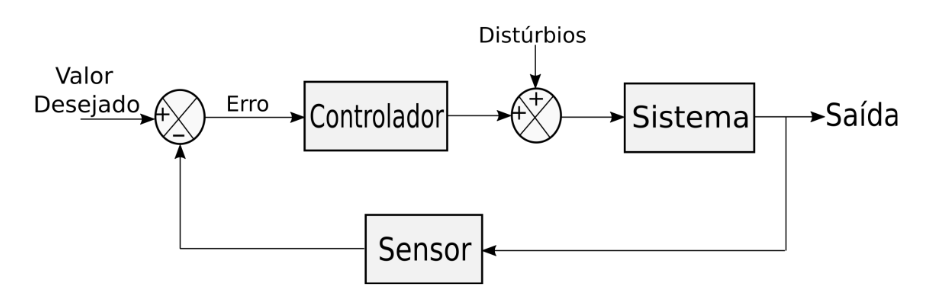
\includegraphics[width=0.9\textwidth]{sist-controle}
	\caption{Sistema Básico de Controle.}
	\label{fig:X}
\end{figure}

Para um professor com mais de cem discentes por semestre, com duas ou mais disciplinas diferentes e com um prazo muitas vezes curto para lecionar todo o conteúdo da disciplina, realizando alguma atividade administrativa e mais pesquisa e extensão, implementar uma abordagem de avaliação ``realimentada'' não é uma tarefa trivial. A seguir, são enumerados alguns métodos de avaliação, detalhados em \citeauthor{elmoresauer}, que podem ser utilizados de forma independente ou para complementar os métodos tradicionais citados no início desta subseção.

\noindent \textbf{One minute paper:} Faltando cinco minutos para o fim da aula, pede-se aos discentes que escrevam sobre o tema abordado em aula por meio da resposta a uma ou duas questões, como as sugeridas por \citeauthor{elmoresauer}.

\begin{itemize}
    \item Quais foram os pontos principais da aula?
\item Quais os pontos menos claros da aula?
\item Qual o conceito mais importante que você aprendeu?
\item Quais perguntas gostaria de fazer?
\item Qual o exemplo, imagem, informação ou ideia mais impactante para você nesta aula?
\item Resolva o(s) seguinte(s) exercício(s) ou problema(s), relativo ao conteúdo visto.
\end{itemize}

A depender das respostas, o professor pode abordar alguns itens no próprio ambiente virtual disponibilizado pela UFOP por meio de fóruns ou disponibilização de material complementar. Além disso, as questões levantadas ou não, servirão de guia para o planejamento da aula seguinte.

\noindent \textbf{Autoavaliação:} Esta avaliação não se trata do discente se dar uma nota, mas sim de avaliar e refletir sobre seu processo de aprendizado antes ou após receber de volta uma prova ou trabalho avaliado. O professor elabora questionários com perguntas que incentivem o discente a autoavaliar e refletir sobre sua dedicação aos estudos, uso das ferramentas e materiais disponíveis, sua motivação e também a dar sugestões que contribuam para seu aprendizado. Esse feedback se torna útil tanto para o discente quanto para o professor.

\noindent \textbf{Avaliação formativa:} Trata-se de propostas que buscam avaliar por meio da promoção do autoconhecimento e de consciência:
\begin{itemize}
    \item Disponibilizar para os discentes as questões de uma prova (por exemplo, no ambiente virtual da UFOP) logo após a realização desta, incentivando o discente a estudar mais os itens em que teve dificuldade na prova e, numa próxima aula, dar a chance deles melhorarem suas respostas na mesma prova tendo um tempo mais reduzido para fazê-lo.
    \item Propor aos discentes a elaboração de resumos sobre o conteúdo estudado feitos com suas próprias palavras, contendo explicações de aula, aplicações do conteúdo estudado, fórmulas, teoremas, regras, passos e qualquer outra informação que achar importante, com exceção de exercícios resolvidos. Esses resumos não podem ser cópias de algum outro autor, devem ter limitação de páginas e podem ser utilizados depois em provas, de modo a serem entregues junto com elas. Essa estratégia também auxilia no desenvolvimento da capacidade do discente de elaborar textos próprios.
    \item Analisar, junto aos estudantes, os resumos elaborados por eles após a devolução da atividade avaliativa. Isso pode ser feito por meio de questões que os levem a refletir sobre a qualidade do resumo elaborado e, assim, melhorar seus métodos de estudo e, consequentemente, os próximos resumos.
\end{itemize}

\noindent \textbf{Análise de erros.} Aqui duas abordagens podem ser adotadas:

\begin{itemize}
\item Devolver as provas corrigidas e dar aos discentes a chance de resolverem novamente, em novo documento, as questões que erraram solicitando que analisem os pontos em que erraram e os justifiquem com base na literatura. A nova solução pode ter caráter substitutivo ou valer uma porcentagem do valor original da questão, a critério do professor.

\item Em aula presencial, após a devolução da atividade avaliada, formar grupos de discentes, contendo em cada grupo pelo menos um discente que teve boa avaliação. Este discente será o líder/orientador do grupo. Cada estudante deve entregar um documento com a solução da questão que errou, contando com a ajuda do colega orientador, valendo uma melhoria na nota da avaliação recebida.

\end{itemize}

\noindent \textbf{Utilizar dos ambientes virtuais} (de preferência aquele disponibilizado pela UFOP) para promover discussões em torno de problemas ou tarefas iniciadas em sala de aula ou propostas, de forma complementar, para serem discutidas somente em ambiente virtual. Aqui, uma maior participação do professor é exigida, promovendo reflexão, argumentação, dedução, dando dicas e incentivando a formação de novas ideias de modo a se chegar na solução do problema. O discente pode ser avaliado de acordo com sua participação no ambiente virtual por meio de:
\begin{itemize}
    \item Perguntas;
    \item Respostas a colegas;
    \item Respostas ao professor;
    \item Conclusão de uma discussão de forma satisfatória.
\end{itemize}

\noindent \textbf{Avaliação pelos pares:} Requer orientação e estabelecimento de critérios pelo professor, principalmente para esclarecer que não se trata de avaliar o colega, mas sua produção e desempenho na realização da tarefa. Este tipo de avaliação traz crescimento para o discente, que desenvolve competências fundamentais para sua vida profissional. O professor pode desenvolver uma ficha de avaliação para o discente, com perguntas pertinentes à atuação do colega avaliado no decorrer do trabalho, bem como a aplicação da nota com as devidas justificativas (aplicável para trabalhos em grupo).

\noindent \textbf{Portfólio físico ou digital:} Trata-se de uma pasta em que se guarda todo o material produzido pelo discente cronologicamente e que pode ser avaliado/autoavaliado posteriormente. No formato digital, com o uso do ambiente virtual disponibilizado pela UFOP que facilita a interação discente-professor, esse método se torna poderoso. Ele possibilita o feedback do professor, bem como acompanhamento da evolução do discente, com cada estudante produzindo no seu tempo, e a possibilidade do compartilhamento em tempo real para todos dos feedbacks caso pertinente.

O novo perfil do discente de engenharia, a grande disponibilidade de informação na Internet, as novas tecnologias de apoio ao ensino, bem como as inovadoras metodologias de ensino, vêm mudando a forma como se ensina e como se aprende, e de forma muito rápida. Deste modo, a maneira como avaliamos o aprendizado deve também se adaptar a essas mudanças se queremos realmente aferir corretamente o aprendizado e utilizar essa informação para a melhoria deste e do próprio ensino de forma contínua e harmoniosa.

Para avaliar estudantes com necessidades específicas, é possível solicitar que produzam material de acordo com suas capacidades, como relatórios em áudio, por exemplo, ou em formato de \textit{PodCast}.

\chapter{Infraestrutura}
\label{cap:07} \index{metodologias}
%
\section{Laboratórios}
\subsection*{Laboratório de Automação Predial}

Tem como objetivo principal o desenvolvimento de projetos e pesquisas relacionados ao conceito de Edifícios Inteligentes, gerando oportunidade de enriquecimento da formação acadêmica para alunos dos cursos de Engenharias e Arquitetura.

As pesquisas desenvolvidas relacionam-se a Sustentabilidade, Eficiência Energética, Climatização de Ambientes, Iluminação Residencial, Comercial e de Monumentos, Conforto Ambiental, e Automação aplicada à edificações, desenvolvendo-se projetos que representem soluções inteligentes, além de buscar trazer um novo olhar para que a comunidade universitária se aproprie dos espaços ao seu redor, experimentando outras formas de ensino, por exemplo, o projeto Laboratório Jardim (LABIM).

Devido a suas características e materiais disponíveis, o Laboratório é ideal para aulas de aplicação prática do conhecimento, de modo que os conceitos teóricos podem ser aprofundados e exemplificados de forma prática.

\subsection*{Laboratório de Acionamentos Elétricos}

Atende a diversos cursos da UFOP, principalmente os cursos de engenharia. Seu principal objetivo é possibilitar a realização de aulas práticas das disciplinas que tenham em sua ementa unidades relacionadas à eletrotécnica. Para tanto, o laboratório conta com recursos e equipamentos como fontes de alimentação ajustável, multímetros, motores CA e CC, resistores de potência, osciloscópios, bancadas didáticas com contatores, relé temporizador, inversor de frequência e lâmpadas.

\subsection*{Laboratório de Controle e Automação Multi-usuário}

O LabCAM, com área de 117 m², possui quatro ambientes internos que são usados para realização de aulas práticas, desenvolvimento de projetos de pesquisa e treinamentos.

O espaço conta com computadores, osciloscópios, geradores de sinais, fontes, analisador de impedância, dentre outros equipamentos.

O laboratório possui uma máquina CNC para execução de projetos de placas de circuito impresso e conta com quatro plataformas didáticas de controle de nível de tanque para realização de aulas práticas de forma remota.

\subsection*{Laboratório de Eletrônica Analógica e Digital}

Seu principal objetivo é possibilitar a realização de aulas práticas das disciplinas do curso que tenham em sua ementa tópicos relacionados a elétrica/eletrônica. Dentre elas, citam-se as disciplinas de Circuitos e Dispositivos Eletrônicos (CAT165) e Acionamentos Elétricos (CAT416), que são disciplinas obrigatórias do curso.

O Laboratório também serve como local de desenvolvimento e testes para projetos de iniciação científica, trabalhos de conclusão de curso e outras pesquisas de alunos relacionados às áreas de controle, automação, eletrônica e acionamentos elétricos. Para tanto, o laboratório conta com recursos e equipamentos como fontes de alimentação ajustáveis, protoboards, osciloscópios, módulos didáticos, multímetros, motores, transformadores, equipamentos para a produção de placas de circuito impresso, dentre outros.

\subsection*{Laboratório de Eletrotécnica}

O Laboratório de Eletrotécnica da Escola de Minas, se não for o primeiro, é um dos mais antigos do Brasil. Constam de seu acervo diversas máquinas e equipamentos elétricos, alguns ainda do século XIX, como, por exemplo, um gerador em anel de Gramme, fabricado em Paris pela empresa Mon~Breguel, entre os anos de 1870 e 1896. Este acervo, extremamente didático, mostra, em suas duas salas, o desenvolvimento da eletricidade ao longo do tempo.

Neste laboratório são lecionadas aulas práticas de Eletrotécnica para os cursos de Engenharia de Minas, Metalúrgica, Civil, Controle e Automação e Mecânica. Nele também são oferecidas aulas práticas para o curso de Arquitetura e Urbanismo e Engenharia Urbana.

Além das aulas práticas de graduação, no Laboratório de Eletrotécnica da Escola de Minas são desenvolvidos diversos trabalhos de pesquisa e de conclusão de curso, bem como cursos de extensão para a comunidade.

Além de diversos geradores e motores de corrente contínua e alternada, transformadores, aparelhos de medida e equipamentos de manobra, o laboratório dispõe de um sistema de geração, elevação, transmissão, rebaixamento e fornecimento de energia elétrica trifásica para alimentar um sistema de iluminação.

A segurança do laboratório é feita por meio de um transformador isolador com neutro flutuante e proteção contra sobrecorrente.

\subsection*{Laboratório de Gestão da Qualidade de Energia}

É dotado de uma subestação abaixadora de tensão alternada com transformadores 13,8Kv/220v ligados em triângulo/estrela para a alimentação dos laboratórios da Escola de Minas.

Além disso, estão nele instalados painéis de controle, supervisão e segurança do sistema. Nos painéis são medidas grandezas como tensão, corrente e fator de potência por meio de equipamentos digitais na saída de cada transformador.

A ideia de transformar a subestação em um laboratório é possibilitar a apresentação de um exemplo de subestação aos alunos para que eles possam ter um primeiro contato com uma instalação desse tipo, assim como os equipamentos nela utilizados.

Importante frisar que o controle e manobra da subestação ainda é manual e que possibilita a implantação de sistemas de controle e manobra automatizado para que seja possível melhorar a segurança e a economia de energia por meio do desligamento de transformadores com baixo consumo (período noturno, férias e finais de semana). Além disso, sistemas de compensação do fator de potência, equilíbrio de fases e harmônicas podem ser estudados, testados e implantados no laboratório.

\subsection*{Laboratório de Metrologia e Instrumentação}

O laboratório conta com uma boa diversidade de equipamentos. Alguns deles são instrumentos de medição de uso geral, tais como: paquímetros, micrômetros, relógios comparadores e termômetros digitais. Outros são mais específicos: medidor de temperatura a laser, rugosímetro e projetor de perfil, e têm sido utilizados em pesquisas. Nas montagens práticas, maletas didáticas de eletrônica são utilizadas no desenvolvimento de protótipos. Além disso, o laboratório conta com osciloscópios, geradores de sinais, sistemas de aquisição de dados, computadores dedicados, entre outros.

São ministradas aulas teóricas e práticas de graduação e mestrado. As aulas práticas incluem, por exemplo, calibração estática e dinâmica de diversos tipos de sensores (e.g., termopares, termistores, LDRs), identificação de sistemas e o desenvolvimento de alguns protótipos de instrumentos. Trata-se, pois, de um espaço dedicado aos alunos para desenvolverem seus trabalhos individuais e/ou em grupo nas áreas de metrologia/instrumentação, controle e automação. Além disso, quando necessário, o laboratório pode ser utilizado para a realização de defesas de Trabalhos de Conclusão de Curso (TCC).

\subsection*{Laboratório de Protótipos e Desenvolvimento de Novas Tecnologias}

O objetivo deste laboratório é a concepção, projeto e construção de protótipos, de forma a atender projetos de P\&D em parcerias com empresas, trabalhos de conclusão de curso de alunos e atender necessidades de outros laboratórios e projetos de pesquisa.

Serão criados cursos de treinamento, de forma a multiplicar conhecimento e tornar os alunos participantes capazes de propor soluções e desenvolve-las a partir da sua formulação até a construção do sub-sistema em forma de protótipo documentado.

\subsection*{Laboratório de Tecnologias Industriais}

Este laboratório atende as aulas de Informática Industrial e Sistemas de Manufatura e também é a casa da equipe Rodetas Robô Clube de Futebol de Robôs, que desde 2011 vem desenvolvendo atividades neste laboratório.

Neste laboratório são desenvolvidas diversas atividades que envolvem o uso de CLP, Sistemas Supervisórios, robôs e plantas didáticas, com o intuito de assimilar as atividades que os futuros engenheiros encontrarão no ambiente industrial.

\subsection*{WebLab Gorceix}

É composto por um conjunto de bancadas reais para práticas de instrumentação, identificação de sistemas e controle de processos à distância. Os equipamentos estão instalados no Laboratório de Controle e Automação Multiusuário (LabCAM).

É um laboratório remoto e está em contínuo desenvolvimento. Atualmente, encontram-se em operação duas bancadas para o controle de nível do processo de dois tanques acoplados, disponíveis para acesso por meio dos seguintes endereços: http://200.239.164.224/ e http://200.239.165.38/. Dessas, a primeira, que foi desenvolvida por Luiz Otávio Mendes, iniciou a operação em 28 de junho de 2016.

Outras três bancadas estão em processo de desenvolvimento para práticas à distância de: (1) controle de velocidade de motor de corrente contínua; (2) controle de temperatura em um túnel de vento; e (3) robótica móvel.

\section{Bibliotecas da UFOP}
O discente terá à sua disposição o sistema de bibliotecas da UFOP, o qual é gerenciado pelo sistema SISBIN (Sistema de Informação de Bibliotecas). Poderá também consultar e retirar livros em qualquer biblioteca do sistema.

A principal biblioteca disponível para os discentes é a Biblioteca da Escola de Minas (EM), a qual dispõe de títulos na área básica de Engenharia Mecânica, Programação, Engenharia de Controle e Automação, Processos de Fabricação, Engenharia Metalúrgica, Engenharia de Minas, Engenharia Civil e Engenharia de Produção, contendo acervo atualizado, com mais de $13.518$ títulos e $27.518$ exemplares, e condizente em número e conteúdo com as disciplinas e linhas de pesquisa propostas, e estatística mensal de $3.800$ empréstimos.

O sistema de bibliotecas da UFOP conta ainda com a Biblioteca do Instituto de Ciências Exatas e Biológicas (ICEB), criada em $1982$, ocupando hoje uma área total de $1050 m^{2}$, distribuída em dois andares, com quinze cabines de estudos individuais e salas de estudo em grupo, mais seis computadores destinados aos usuários e doze computadores no total, com acervo de aproximadamente $8.502$ títulos e $22.433$ exemplares, e estatística mensal de $15.000$ empréstimos.

Ambas as bibliotecas dispõem de um espaço amplo e bem ventilado para atender aos discentes, com salas de estudo individuais e em grupo. As bibliotecas em conjunto dispõem de mais de 1.200 títulos nas áreas acima citadas.

O sistema também conta com a Biblioteca Prof. Luciano Jacques de Moraes (DEGEO/DEMIM) e a Biblioteca de Obras Raras da Escola de Minas – BIBORAR. Aquela possui acervo de $12.000$ livros e $90$ títulos de periódicos nacionais e internacionais, e conta ainda com uma mapoteca que disponibiliza cerca de $2.600$ mapas topográficos e geológicos. Esta reúne cerca de $22000$ volumes de publicações técnico-científicas nas áreas de ciências naturais, puras e aplicadas, que incluem livros e periódicos raros, enciclopédias, guias, manuais e legislação, editados entre os séculos XVII ao XX, no Brasil e no exterior. A Biblioteca guarda ainda a Coleção Carlos Walter e a Coleção Ex-discentes e Ex-professores da Escola de Minas, acervos bibliográficos de renomados profissionais que passaram pela instituição.

A Universidade Federal de Ouro Preto faz parte da rede do Portal de Periódicos CAPES. Desta forma, os estudantes terão acesso a textos completos, incluindo os periódicos e anais de congressos da ACM (Association for Computing Machinery) e os periódicos e anais de congressos do IEEE (Institute of Electrical and Electronics Engineers).

Os estudantes poderão utilizar também os laboratórios de informática da Escola de Minas e do Departamento de Ciência da Computação (DECOM). O primeiro laboratório, compartilhado com os cursos instalados na Escola de Minas, possui área física aproximada de $60m^{2}$, e conta com $30$ computadores. Neste laboratório, monitores atendem os discentes fora do horário de aulas. Já o laboratório do DECOM é de uso comum para os cursos de Engenharia, e possui capacidade para atendimento de $60$ discentes. O laboratório também é equipado com datashow, e disponibiliza monitores para atendimento aos discentes fora do horário de aulas.
%
\section{NITE}
Em 2001 a UFOP criou o Núcleo de Inovação Tecnológica e Empreendedorismo (NITE), com o intuito de promover a formação de um ambiente cooperativo que conjugue interesses da UFOP, empresas e órgãos para promoção de atividades inovadoras e de transferência de tecnologia, com vistas a contribuir para o desenvolvimento social e econômico da região de influência e da Instituição.

Os principais objetivos do NITE são captar e proteger os ativos de propriedade intelectual gerados na UFOP, formar parcerias com empresas e com organizações, a fim de transferir esses ativos ao mercado para o uso público e para o desenvolvimento econômico e implementar a cultura empreendedora no ambiente acadêmico como um todo.

Atualmente, o NITE está dividido em seis setores distintos, pois visa facilitar a implementação das ações propostas, direcionando os planos e ações para cada setor específico.

\chapter{Concepção do curso}
A concepção do curso se estabelece a partir da missão de produzir e disseminar o conhecimento científico, tecnológico, social, cultural, patrimonial e ambiental, contribuindo para a formação do sujeito como profissional ético, crítico-reflexivo, criativo, empreendedor, humanista e agente de mudança na construção de uma sociedade justa, desenvolvida socioeconomicamente, soberana e democrática. Além disso, à luz dos princípios constitucionais e das finalidades estatutárias, guia-se pelos valores que pautam a atuação da UFOP: autonomia; compromisso, inclusão e responsabilidade social; criatividade; democracia, liberdade e respeito; democratização do ensino e pluralização do conhecimento; eficiência, qualidade e excelência; equidade; indissociabilidade; integração e interdisciplinaridade; parcerias; preservação do patrimônio artístico, histórico e cultural; saúde e qualidade de vida; sustentabilidade; e transparência.

A presente proposta de reforma curricular está ancorada em pressupostos e ideias em consonância com as Diretrizes Curriculares Nacionais para os Cursos de Graduação em Engenharias e com os princípios institucionais estabelecidos no PDI e no PPI da Universidade Federal de Ouro Preto. Tem-se como objetivo atender as referidas DCNs mantendo-se e realçando-se as qualidades do curso de Engenharia de Controle e Automação da UFOP. Nesse contexto, os seguintes documentos e discussões basearam a presente proposta:

a. Diretrizes Curriculares Nacionais para os cursos de Engenharia de Controle e Automação (Res. CNE/CES Nº 1, DE 6 DE JANEIRO DE 2015, Anexo 1) e para os cursos de Engenharia (Res. Resolução CNE Nº1/2021);

b. Diretrizes para a Extensão na Educação Superior Brasileira (Resolução nº7/2018).

c. Política Institucional de Formação para os cursos de Engenharia da Universidade Federal de Ouro Preto
d. Reuniões do NDE e do Colegiado de Curso.


Com base em todos os pressupostos analisados, a presente proposta tem três pilares conceituais importantes:

i. o discente deverá ser o agente principal da sua formação: diferentemente do formato atual, o que se espera é um comportamento ativo do discente no processo educacional, deixando de lado o modelo atual, com elevada carga horária obrigatória em sala de aula;

ii. o curso formará Engenheiros de Controle e Automação para atuarem nos diversos campos da Engenharia de Controle e Automação, assim como na interface com as áreas da Engenharia;

iii. a base da formação dos estudantes deverá ser constituída de conhecimentos fundamentais da Engenharia de Controle e Automação.

O curso será estruturado da seguinte forma: um núcleo básico de disciplinas de Engenharias, concomitantes com um núcleo de conteúdos básicos em Controle e Automação. A estes dois núcleos segue-se um núcleo profissionalizante.

O curso está estruturado por meio do encadeamento e política de pré-requisitos lógicos entre as disciplinas, estabelecidos na matriz curricular e, por meio de disciplinas eletivas, que devem estar em constante atualização, os discentes poderão estabelecer seu planejamento acadêmico.
%
\chapter{Mobilidade acadêmica}
Os processos que permitem mobilidade acadêmica aos nossos estudantes proporcionam uma experiência com formas diversas de ensino e aprendizagem, com pesquisas de ponta e tecnologias em desenvolvimento. Os estudantes em mobilidade acadêmica têm a oportunidade de viver realidades diversas que vão impactar tanto sua trajetória acadêmica como sua vida profissional, possibilitando, também, que os estudantes que não estiveram em mobilidade possam conhecer, por meio de relatos, as experiências vividas. A mobilidade acadêmica permite, ainda, o contato com culturas e manifestações diversas, proporcionando a ampliação do olhar e a relação com o diferente.

\chapter{Capacitação do corpo docente}

O corpo docente do curso de Engenharia de Controle e Automação é composto majoritariamente por Doutores sendo que a capacitação é realizada de acordo com a política institucional que estabelece as diretrizes e os procedimentos para a execução das ações de capacitação e qualificação que visam o aprimoramento constante do ensino, pesquisa e extensão. A UFOP promove, através de sua política institucional, a qualificação da docência no ensino superior com diversas ações voltadas para o aprimoramento da experiência docente nas temáticas de metodologia de ensino, prática da extensão, avaliação, relação professor/aluno e currículo. Há ainda por meio da instituição ações de incentivo à qualificação dos docentes, através do auxílio à qualificação; incentivo par afastamento para participação em Programas de Pós-graduação stricto sensu, concessão de jornada especial de trabalho para docentes que estão em processo de capacitação, licença específica para capacitação e incentivo à participação em Programas de
Pós-Graduação na UFOP.

Dentre as ações supracitadas, destaca-se, de forma mais específica, a contínua formação de docentes desenvolvidas no âmbito do ``Programa Sala Aberta'', do Núcleo de Apoio Pedagógico (NAP) da UFOP. Tal programa visa a ampliação dos espaços para diálogos e reflexões sobre os desafios da docência universitária, tendo como protagonistas os docentes. Quando do ingresso do Servidor Público, a intuição realiza ações de integração, de participação obrigatória, para que os trabalhadores recém chegados tenham a visão global da Instituição, mas também tenham os devidos esclarecimentos sobre as responsabilidades, direitos e deveres e as especificidades do serviço público. São realizadas também ações de gestão, focadas em preparar ou atualizar os servidores da UFOP para atividades administrativas e de gestão. Ressalta-se que todas essas atividades de capacitação são amplamente divulgadas pelos setores responsáveis e que o DECAT incentiva os seus servidores a participarem das mesmas.


\chapter{Avaliações promovidas pelo curso}

\section{Avaliações institucionais}

\subsection*{Pesquisa de Desenvolvimento de Disciplinas}

Semestralmente, o desenvolvimento de todas as disciplinas do curso é submetido a avaliação interna. Conforme o Plano de Desenvolvimento Institucional para o período de 2016- 2025, um dos objetivos que deve direcionar as políticas de graduação da universidade consubstancia-se no aprimoramento da Pesquisa de Desenvolvimento de Disciplinas da Graduação, organizada pela Pró-Reitoria de Graduação (PROGRAD), avaliando o instrumento e garantindo a socialização e a discussão periódica dos resultados junto aos coordenadores de curso, colegiados e chefias de departamento. A execução da pesquisa é realizada pelo Núcleo de Apoio Pedagógico (NAP), órgão vinculado à PROGRAD, também responsável pelo seu acompanhamento.
No âmbito das disciplinas do Curso de Engenharia de Controle e Automação, a coordenação do curso, docentes e a representação discente estão envolvidos e comprometidos em estimular a comunidade acadêmica (discentes e docentes) a atender ao convite para o adequado preenchimento dos formulários eletrônicos das avaliações periódicas. Objetiva-se, com isso, a obtenção de resultados representativos, quantitativa e qualitativamente, que viabilizem o feedback aos interessados e o direcionamento de ações de aperfeiçoamento permanente.

\subsection*{Comissão Própria de Avaliação}

A avaliação interna é realizada pela Comissão Própria de Avaliação Institucional da EM (CPAI-EM) e Comissão Própria de Avaliação (CPA) da Universidade Federal de Ouro Preto, conforme determina a Lei nº 10.861, de 14 de abril de 2004, que institui o Sistema Nacional de Avaliação da Educação Superior (SINAES). A CPAI-EM está regulamentada pela Resolução CUNI No. 2459, de Setembro de 2021, que aprova o regimento interno da Escola de Minas (Seção IX), enquanto a CPA está regulamentada pela Resolução CEPE nº 2.680, alterada pela Resolução CEPE nº 2.826, que aprova o Regimento Geral da Comissão Própria de Avaliação da UFOP. Estes órgãos mantém contato com todos os segmentos da comunidade acadêmica e procura fazer diagnóstico permanente das atividades curriculares e extracurriculares, a fim de verificar se atendem às necessidades da sociedade, do DECAT e da UFOP. Além disso, propõe mudanças no projeto político-pedagógico, ouvindo os(as) alunos(as), professores(as) e servidores(as) técnico-administrativo em educação, estimulando-os a participarem ativamente do processo de avaliação.


\subsection*{Avaliações externas}
As avaliações externas à UFOP têm como normatização básica a Lei 10.861, de 14 de abril de 2004, que instituiu o Sistema Nacional de Avaliação da Educação Superior (SINAES). Além disso, em 2018, o Ministério da Educação alterou seus Instrumentos de Avaliação de Cursos de Graduação (INEP/MEC). O Instrumento de Avaliação é a ferramenta que contém informações, contextualização da IES, do curso, eixos, dimensões, indicadores e critérios de análise associados, a serem observados pela Comissão Avaliadora antes da visita e no ato de verificação das condições de funcionamento de cursos de graduação e instituições de ensino superior. Nesse contexto, o relatório de avaliação embasa decisões do MEC e da própria IES avaliada (INEP/MEC, 2018).

%
% ---
% ----------------------------------------------------------
% PARTE
% ----------------------------------------------------------
%\part{Documentos}
% ----------------------------------------------------------
% ---
% Capitulo de revisão de literatura
% ---
% ----------------------------------------------------------
% PARTE
% ----------------------------------------------------------
%\part{Resultados}
% ----------------------------------------------------------
% ---
% primeiro capitulo de Resultados
%\include{anexos/capitulo-resultados}
% ----------------------------------------------------------
% Finaliza a parte no bookmark do PDF
% para que se inicie o bookmark na raiz
% e adiciona espaço de parte no Sumário
% ----------------------------------------------------------
\phantompart
% ---
% Insere arquivo de Considerações Finais ou Conclusões
% ---
%\include{anexos/capitulo-consideracoes-finais}
% ----------------------------------------------------------
% ELEMENTOS PÓS-TEXTUAIS
% ----------------------------------------------------------
\postextual
% ----------------------------------------------------------

% ----------------------------------------------------------
% Referências
% ----------------------------------------------------------

%\bibliography{referencias-ppc}
%% ----------------------------------------------------------
%% Referências bibliográficas
%% ----------------------------------------------------------
% toca nome de bibliografia para ``Referências''
\printbibliography[title=Referências]

% ----------------------------------------------------------
% Glossário
% ----------------------------------------------------------
%
% Consulte o manual da classe abntex2 para orientações sobre o glossário.
%
% ----------------------------------------------------------
% Apêndices
% ----------------------------------------------------------
%(Lembre-se: Apendices são de autoria do próprio autor do texto.
% Anexos são elementos de autorias de outros, que o autor do texto julga interessante apresentar)

% ---
% Inicia os apêndices:
% ---
%\begin{apendicesenv}

% Imprime uma página indicando o início dos apêndices
%\partapendices % Esse comando gera um warning na compilacao do overleaf
% ---
% Insere arquivo com os apendices A a D
%\end{apendicesenv}
% ---

% ----------------------------------------------------------
% Anexos
% ----------------------------------------------------------

% Inicia os anexos
% ---
%%%%%%%%%%%%%%%%%%%%%%%%%%%%%%%%%%%%%%%%%%%%%início do trecho comentado

\begin{anexosenv}
% Imprime uma pági/a indicando o início dos anexos
%\partanexos
% ---
% Insere arquivo com os anexos 1, 2 e 3
% ---
%%%%%%%%%% ANEXO 1
%

\chapter{Programas de Disciplinas} \label{ape:01}

%Primeiro semestre
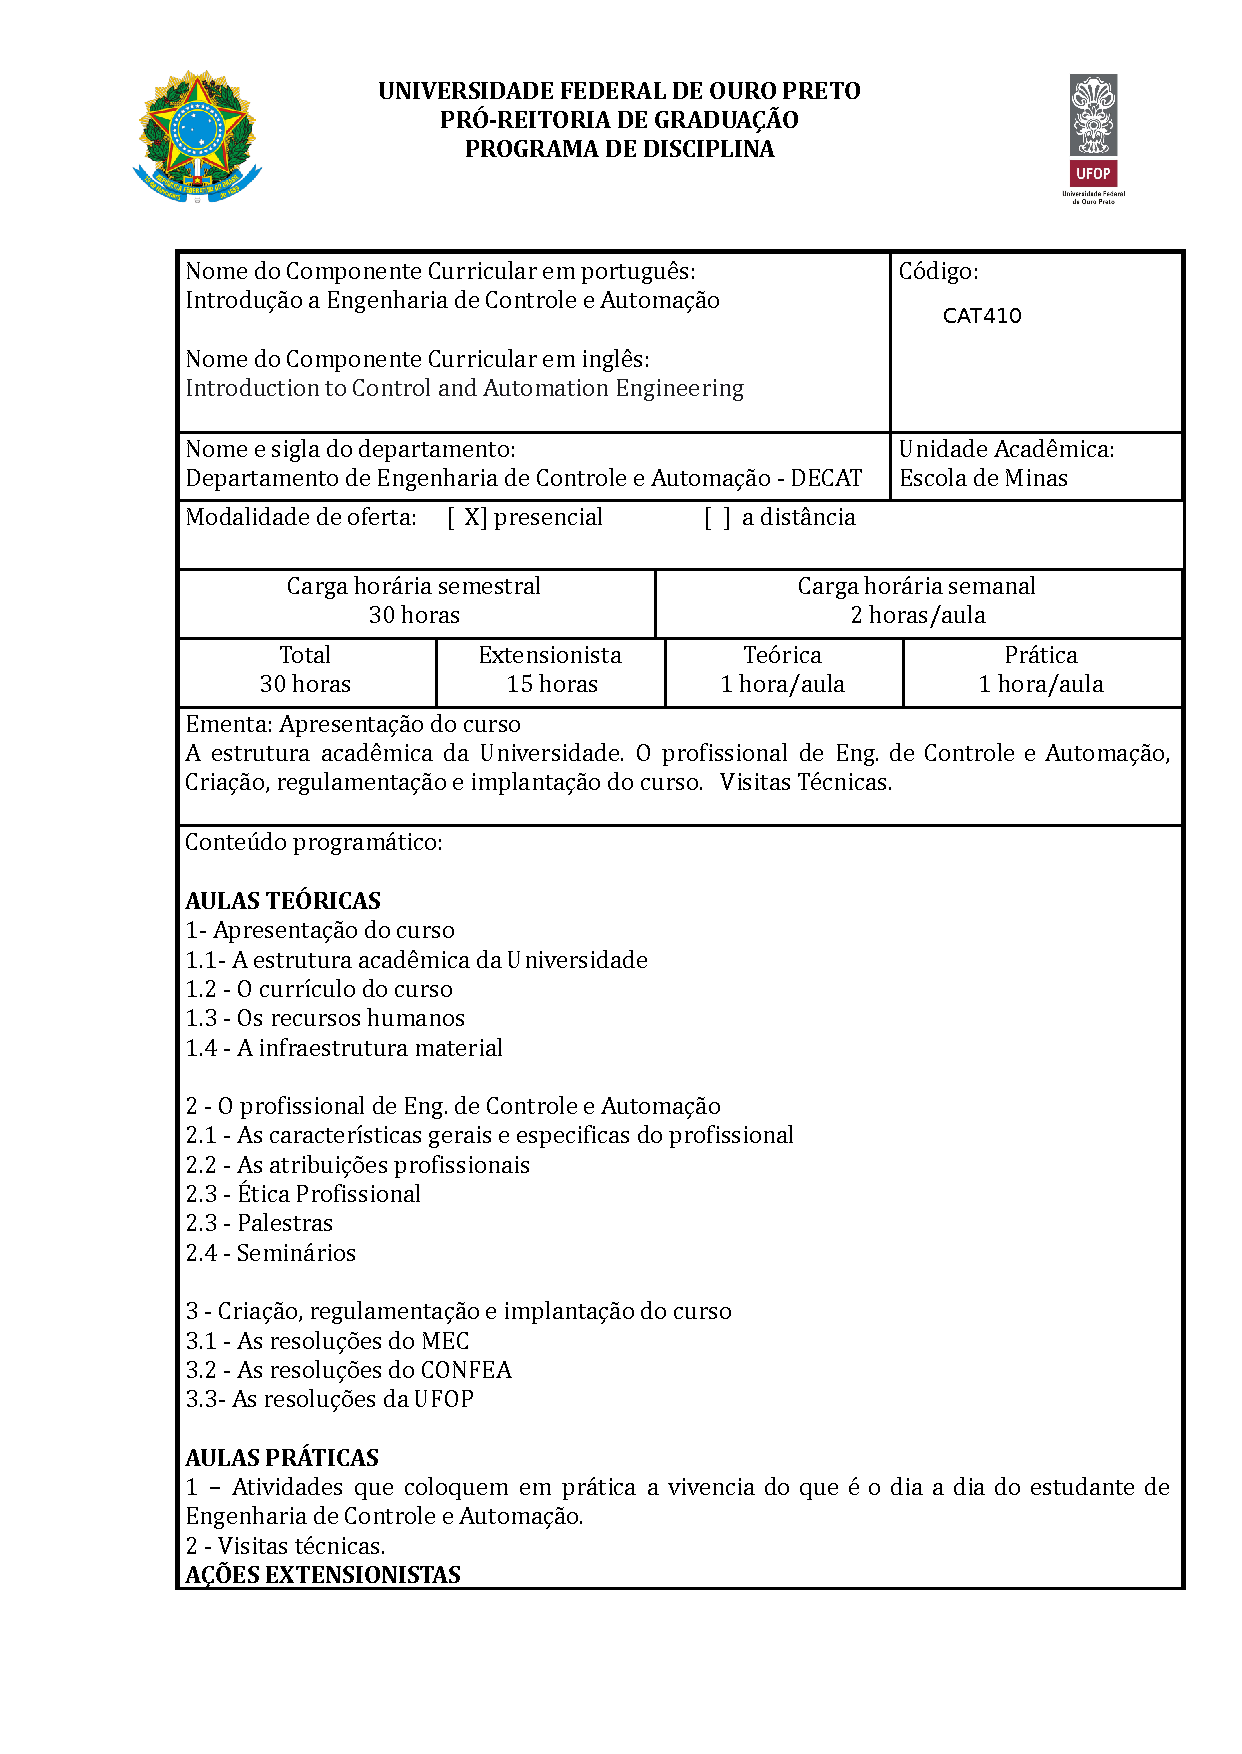
\includepdf[pages=-,nup=1x1, frame]{CAT410} % CAT001
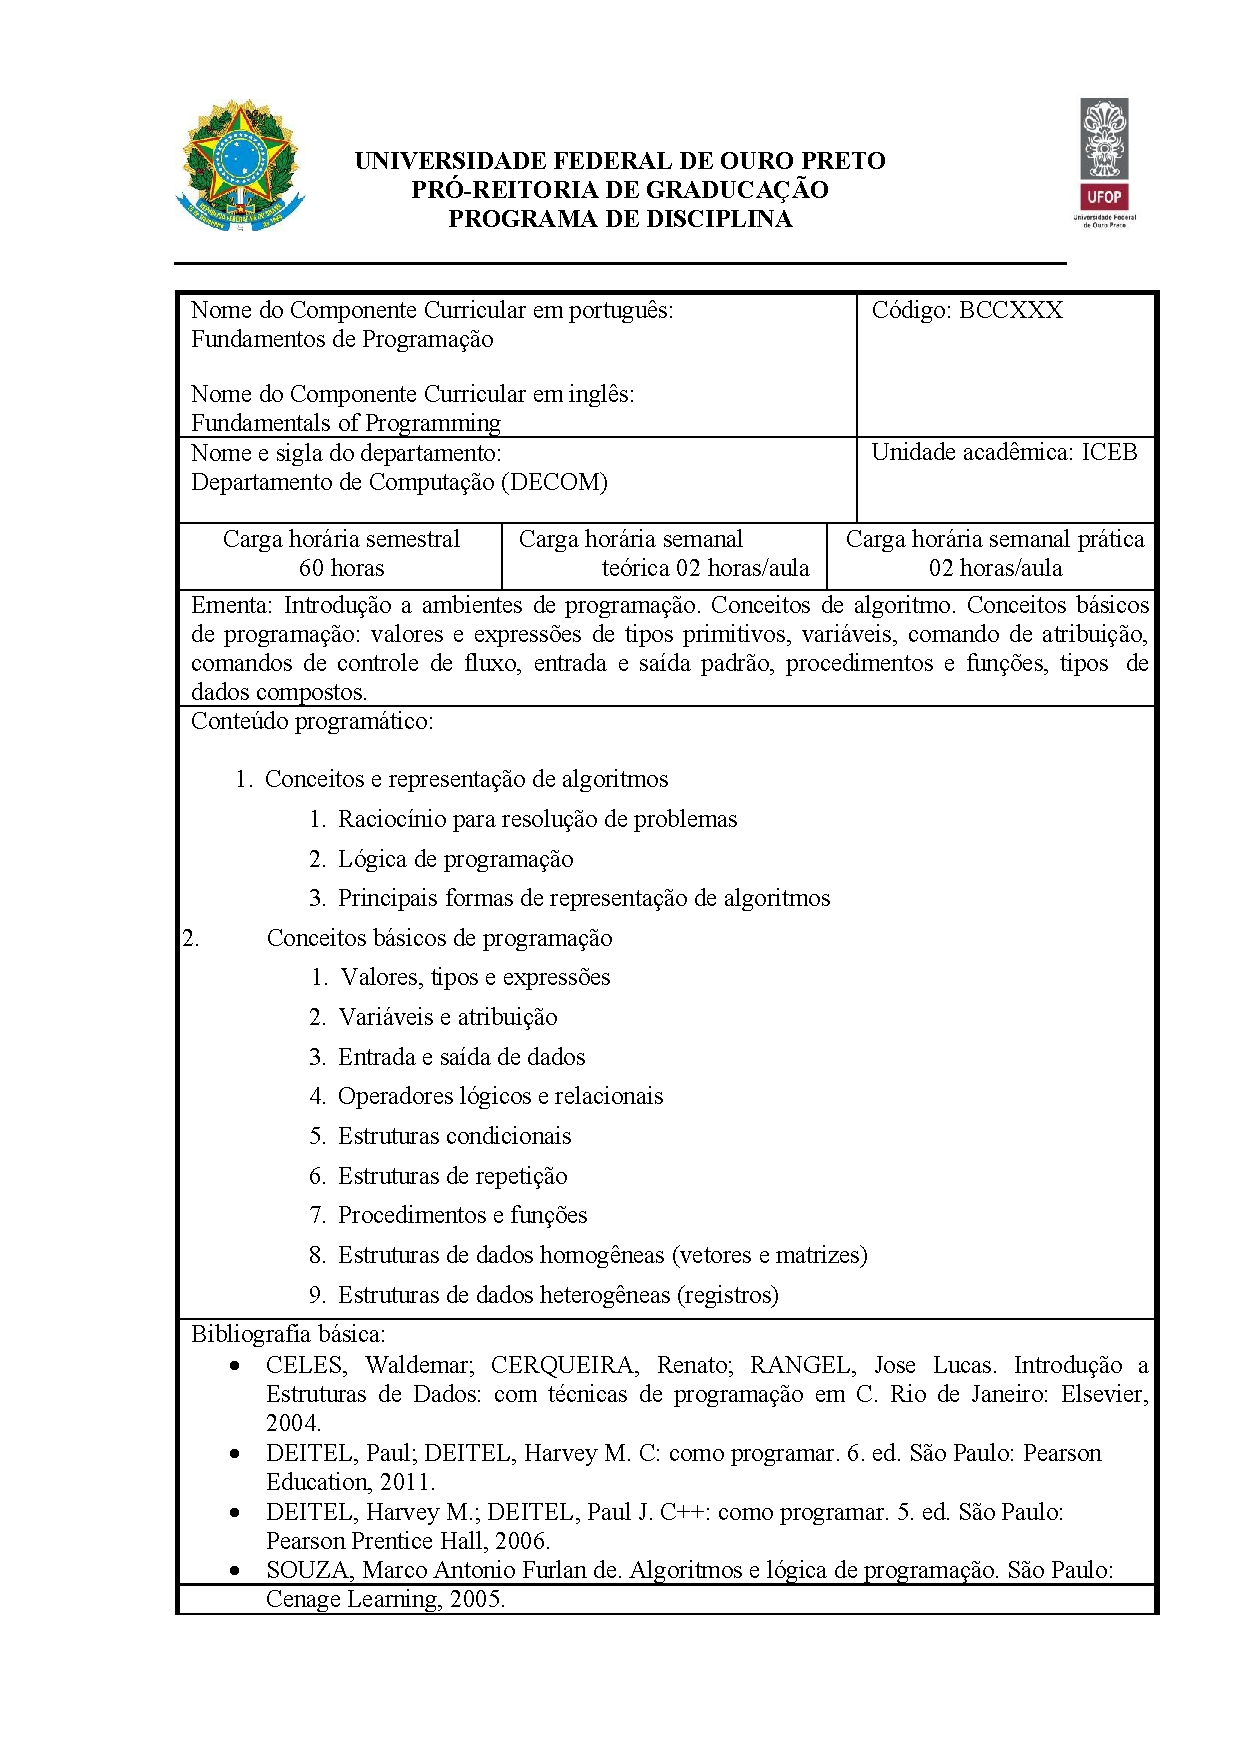
\includepdf[pages=-,nup=1x1, frame]{BCC703}
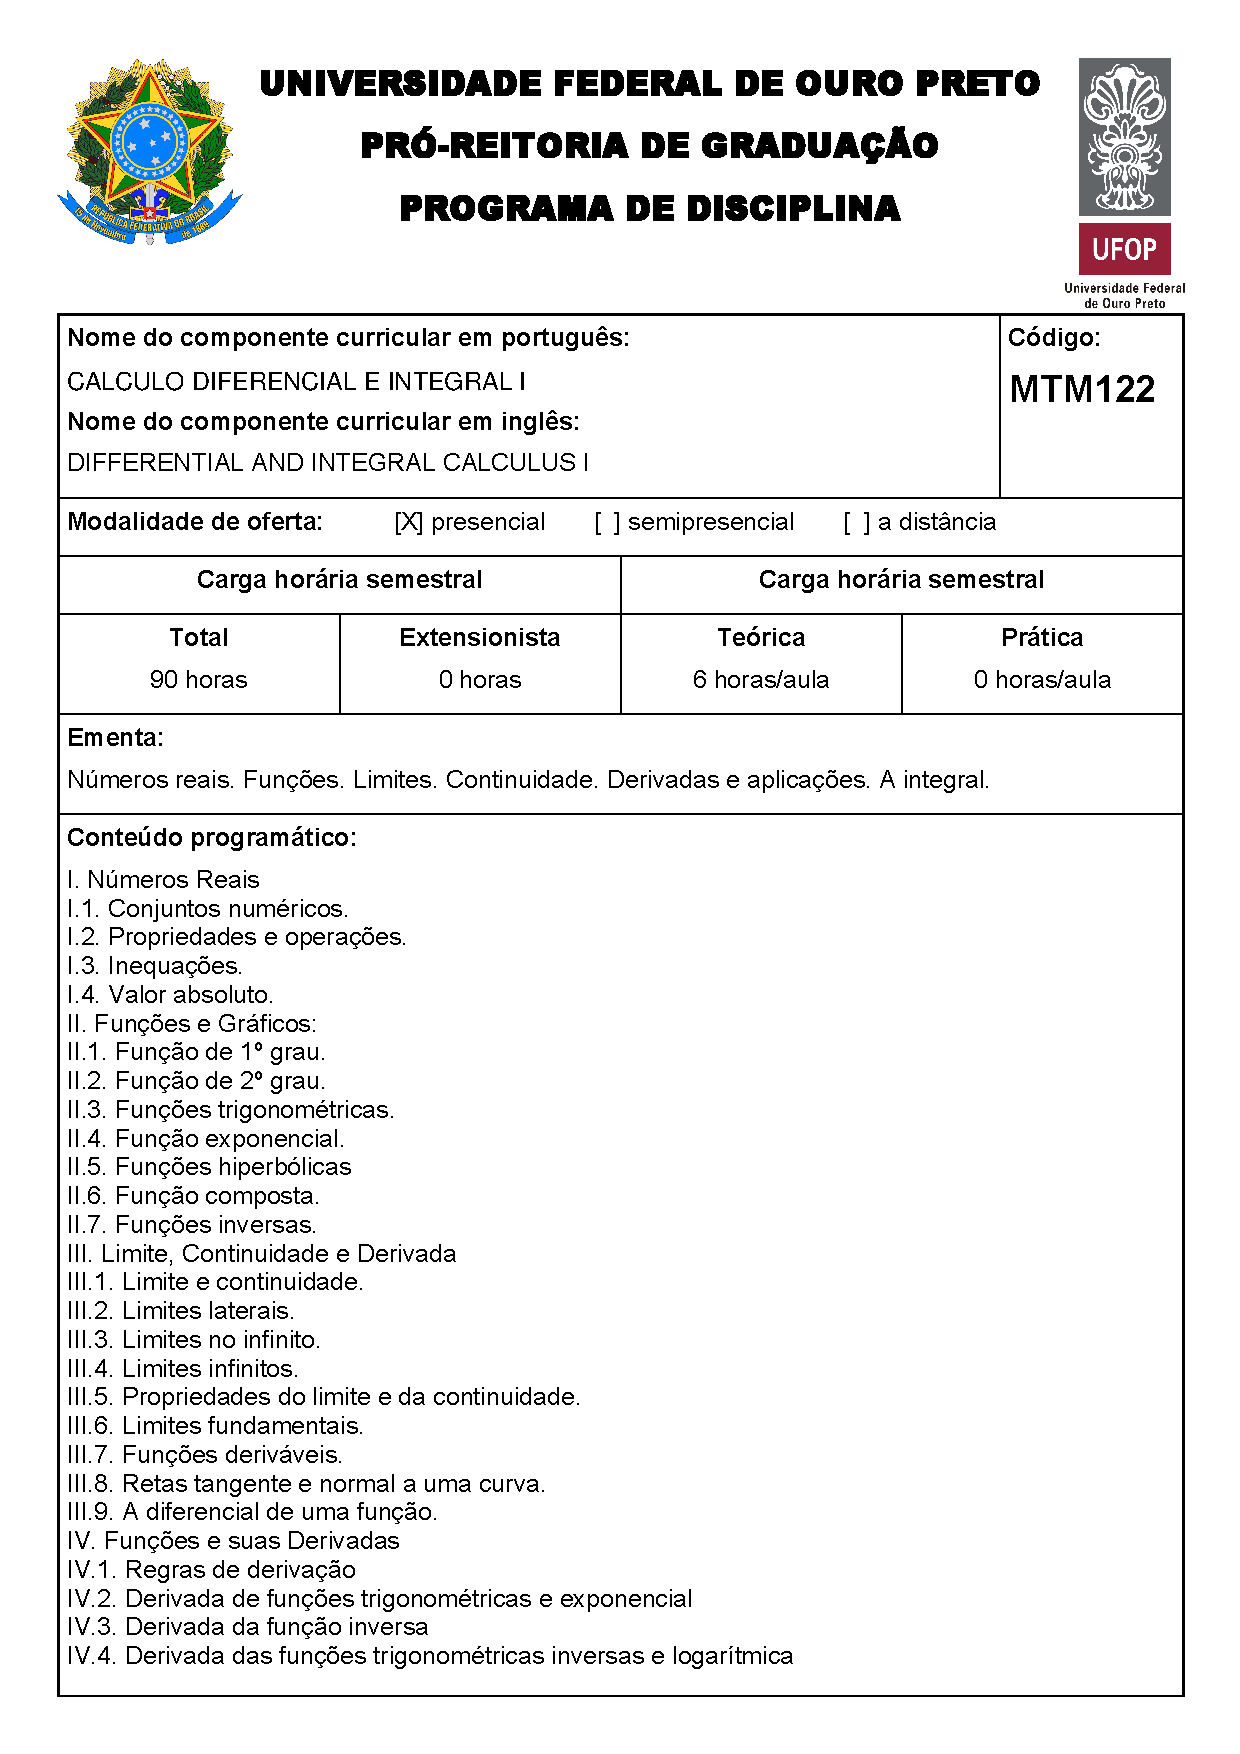
\includepdf[pages=-,nup=1x1, frame]{MTM122}
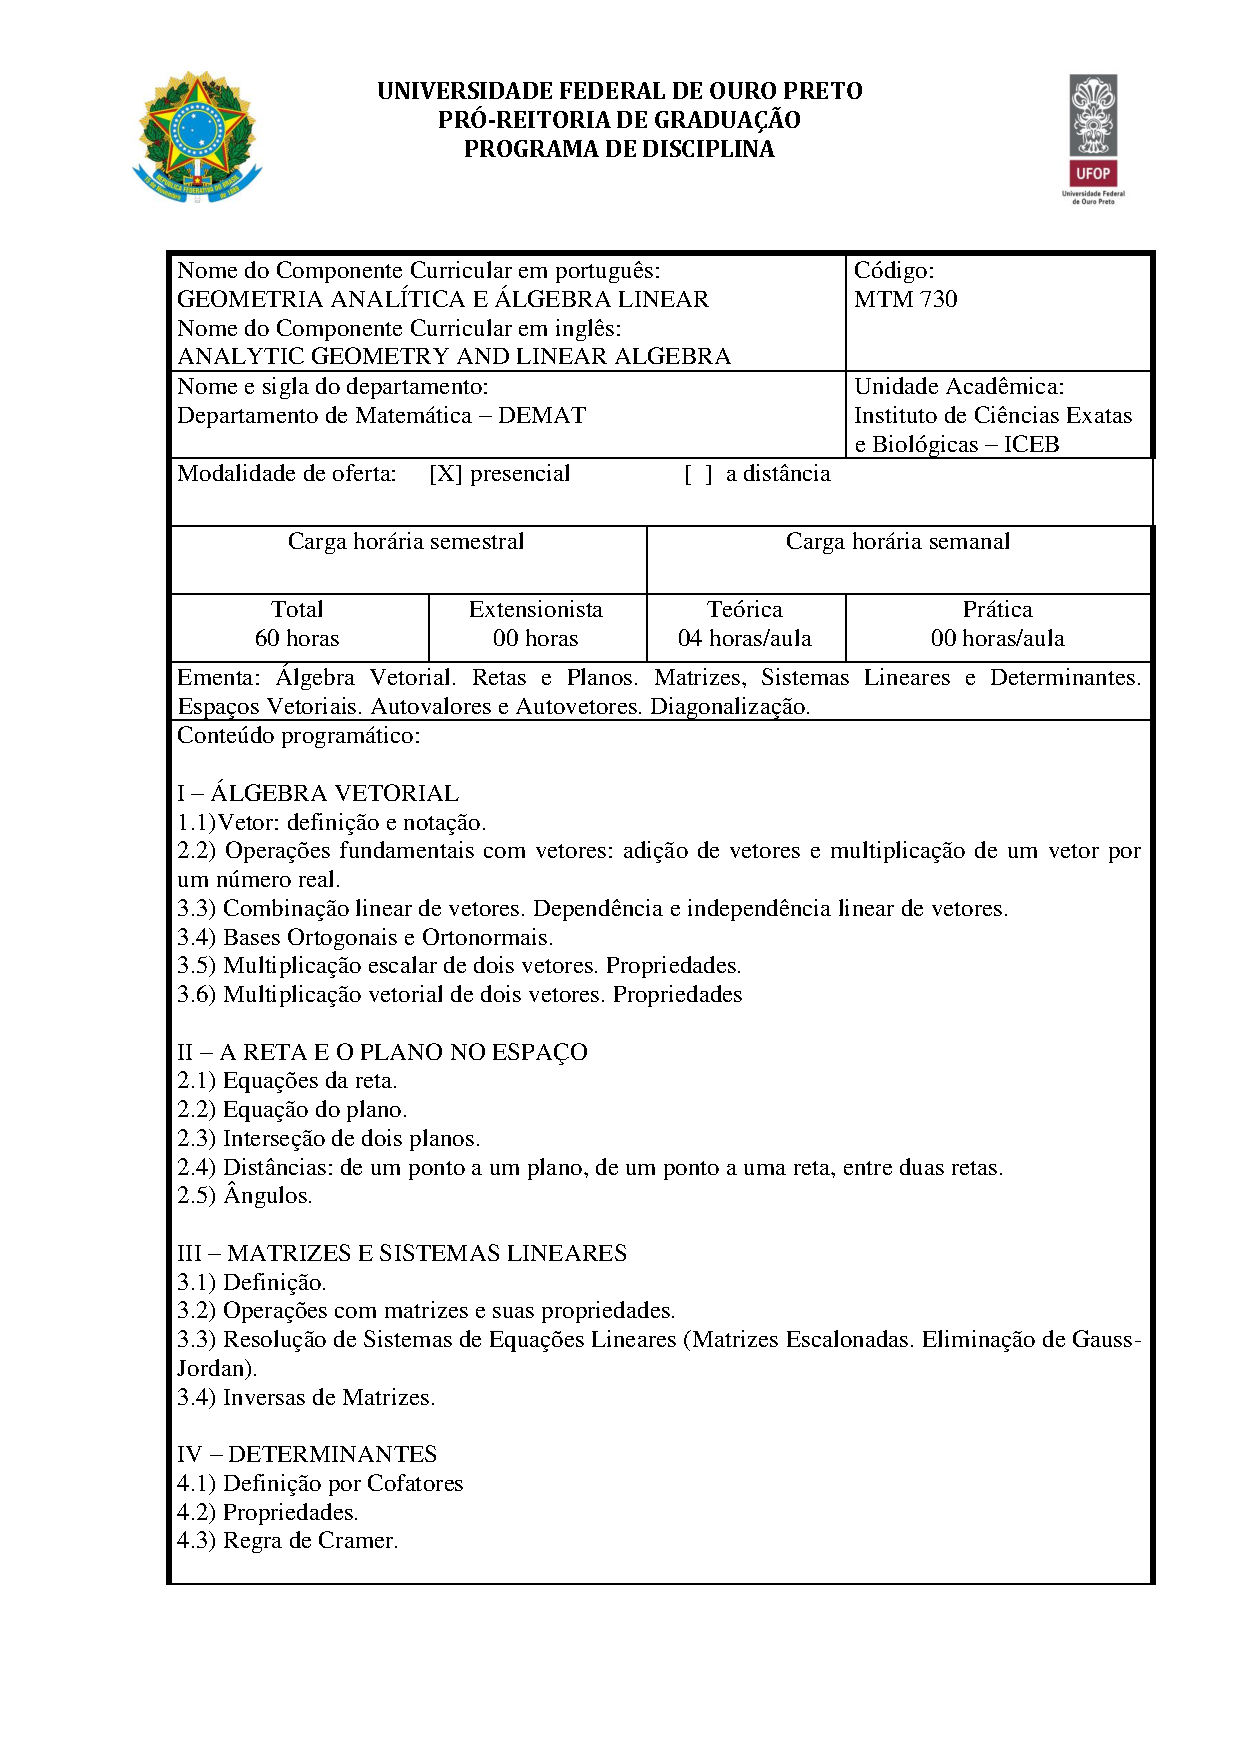
\includepdf[pages=-,nup=1x1, frame]{MTM730}
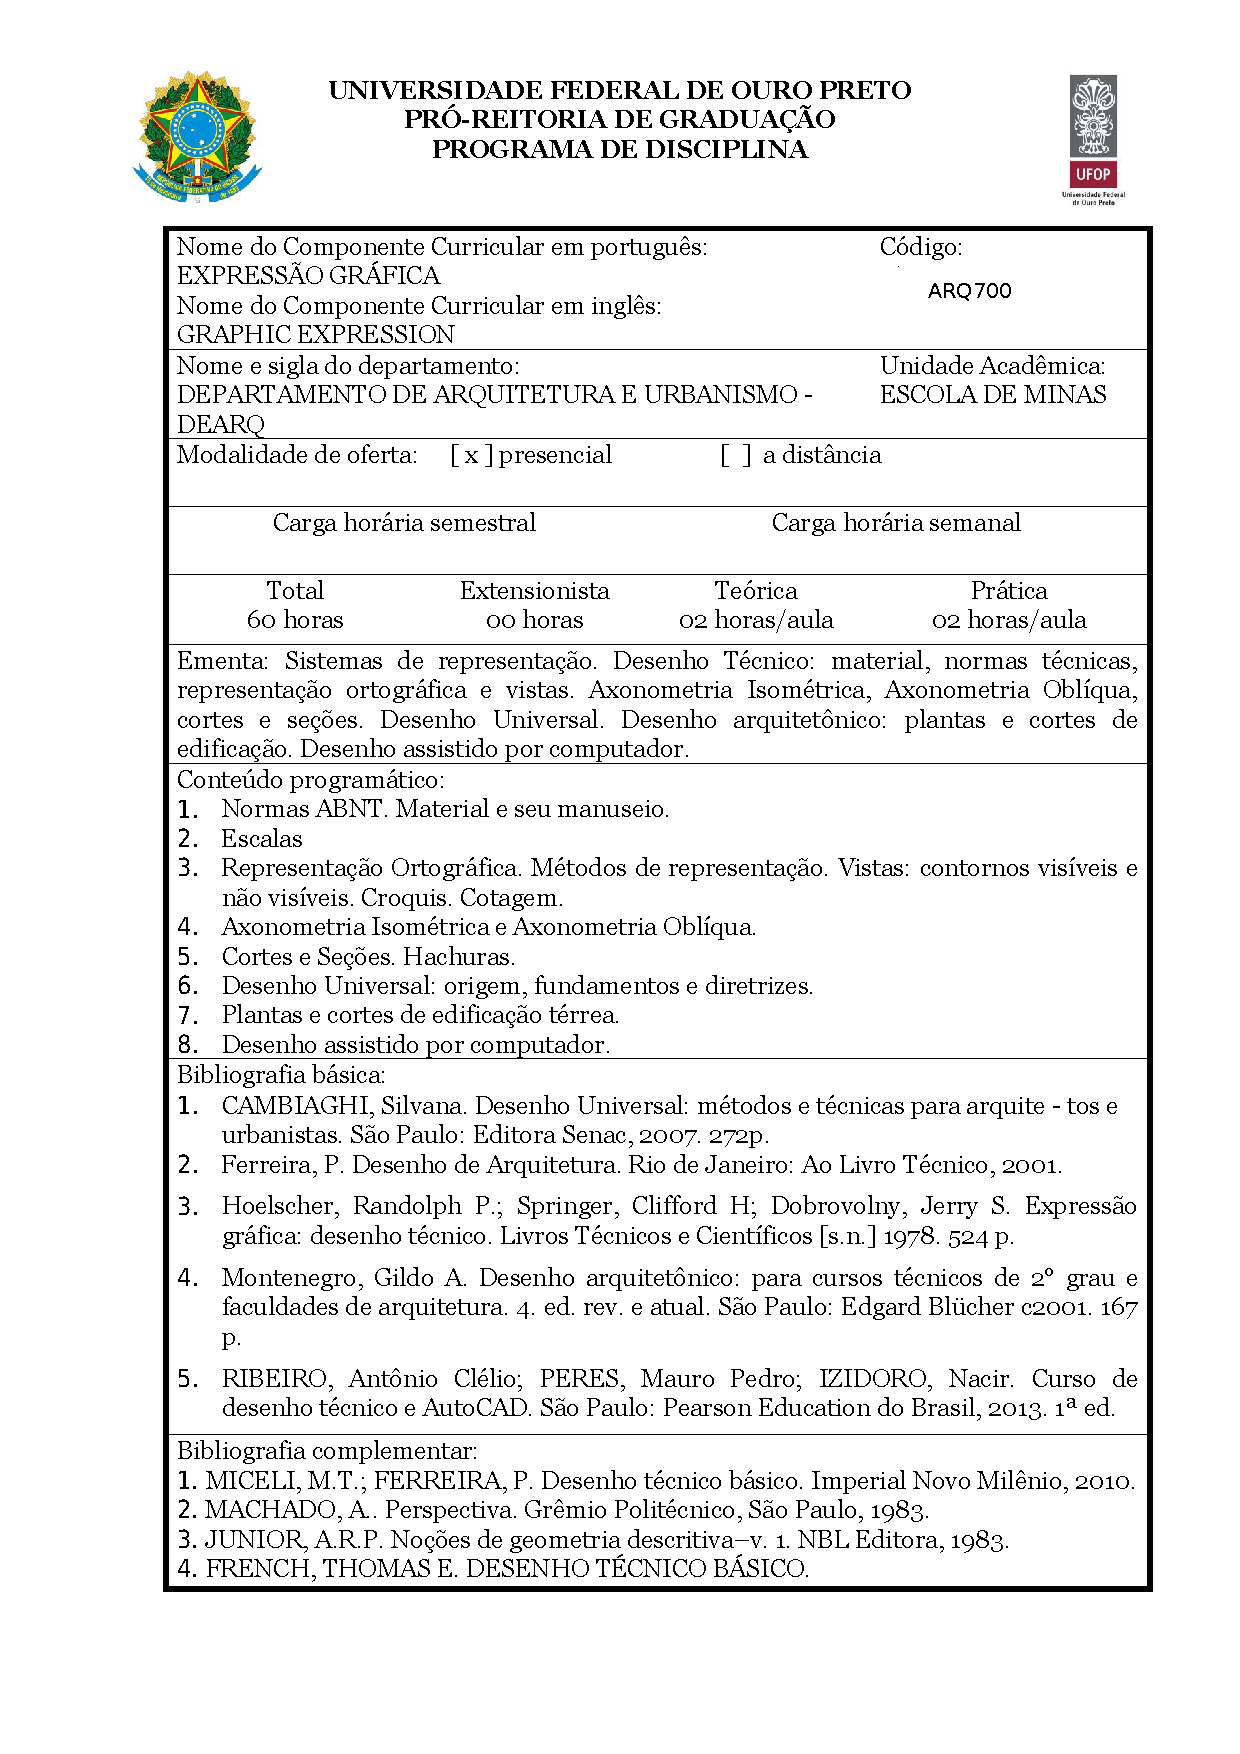
\includepdf[pages=-,nup=1x1, frame]{ARQ700}

%%%%% COMENTADO A PARTIR DAQUI DADO QUE O OVERLEAF
%%%%% TEM DIFICULDADES DE COMPILAR PROJETOS MAIORES
%%%%%  FAVOR COMPILAR EM UM EDITOR OFFLINE
%\begin{comment}

%Segundo semestre
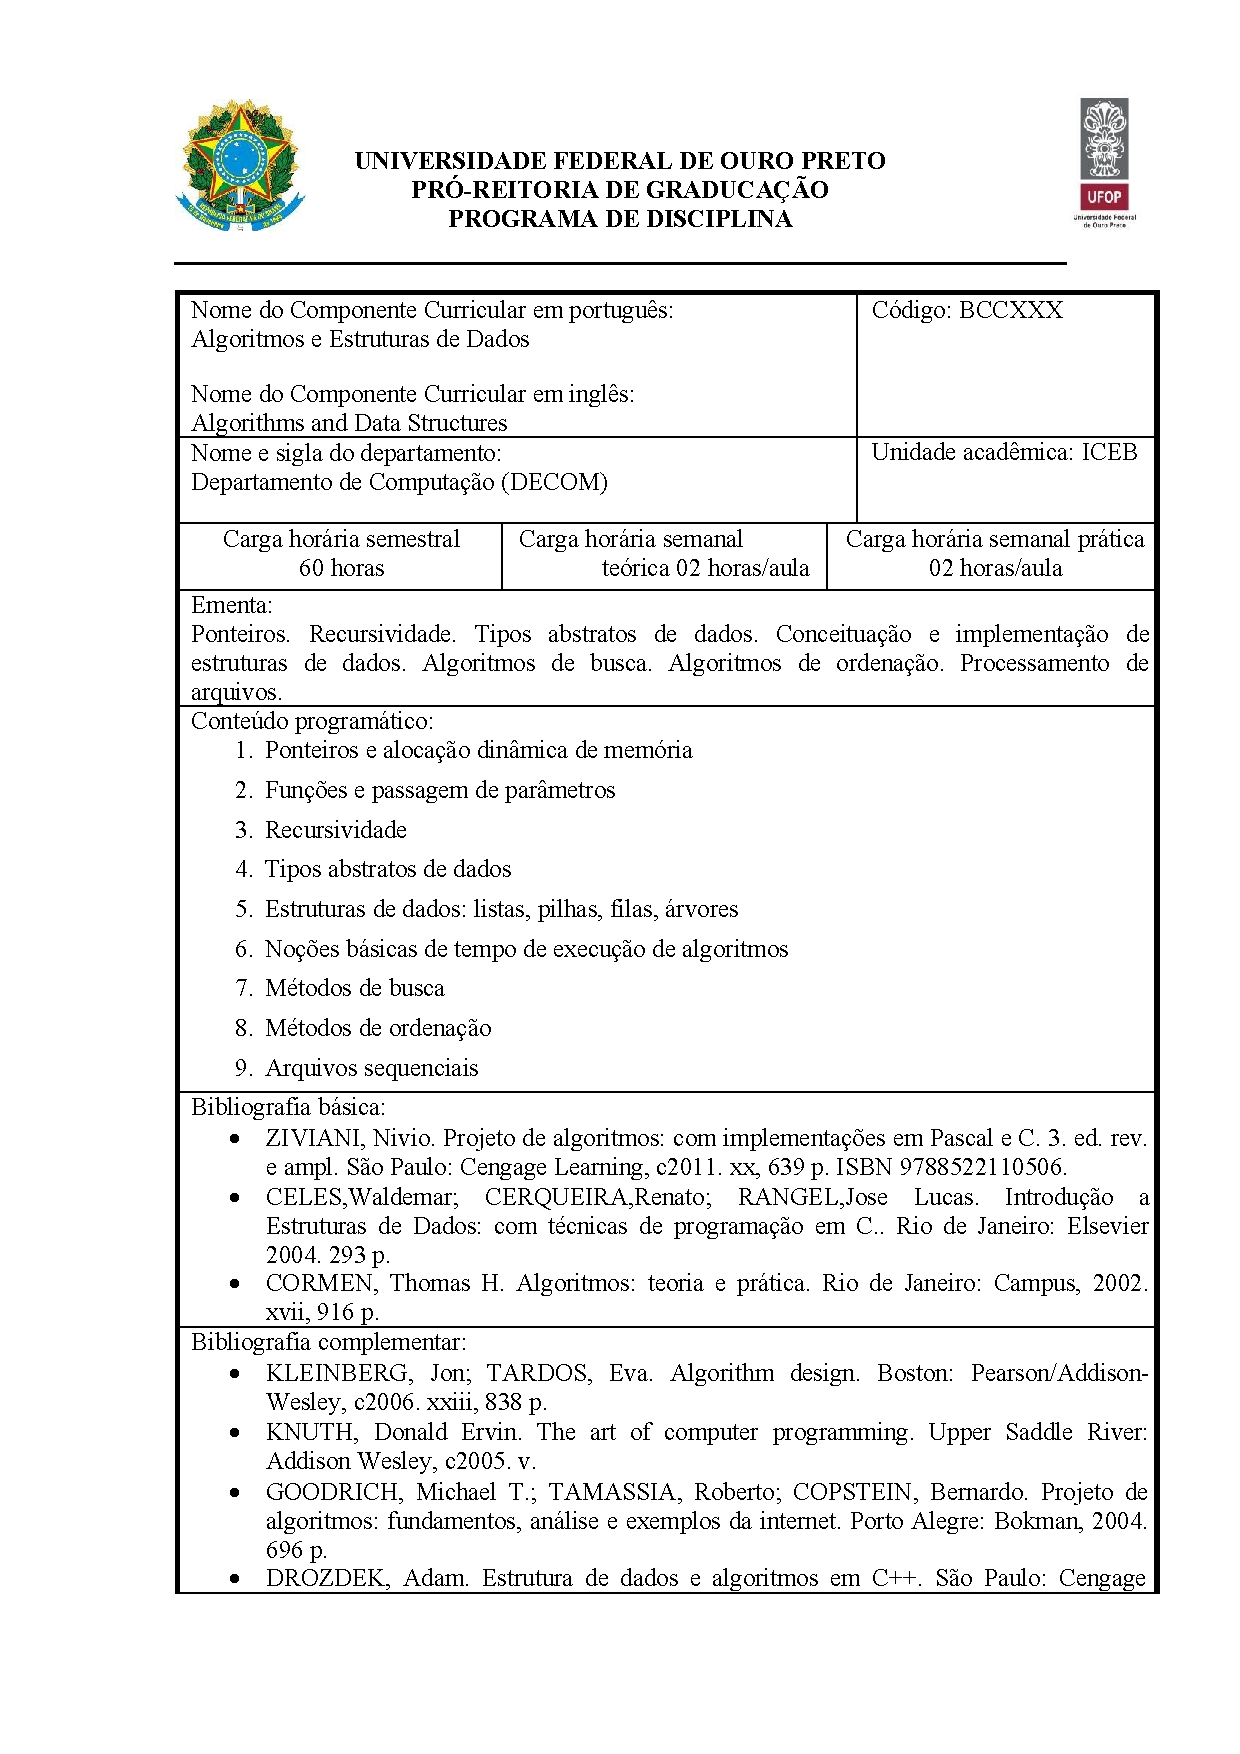
\includepdf[pages=-,nup=1x1, frame]{BCC704}
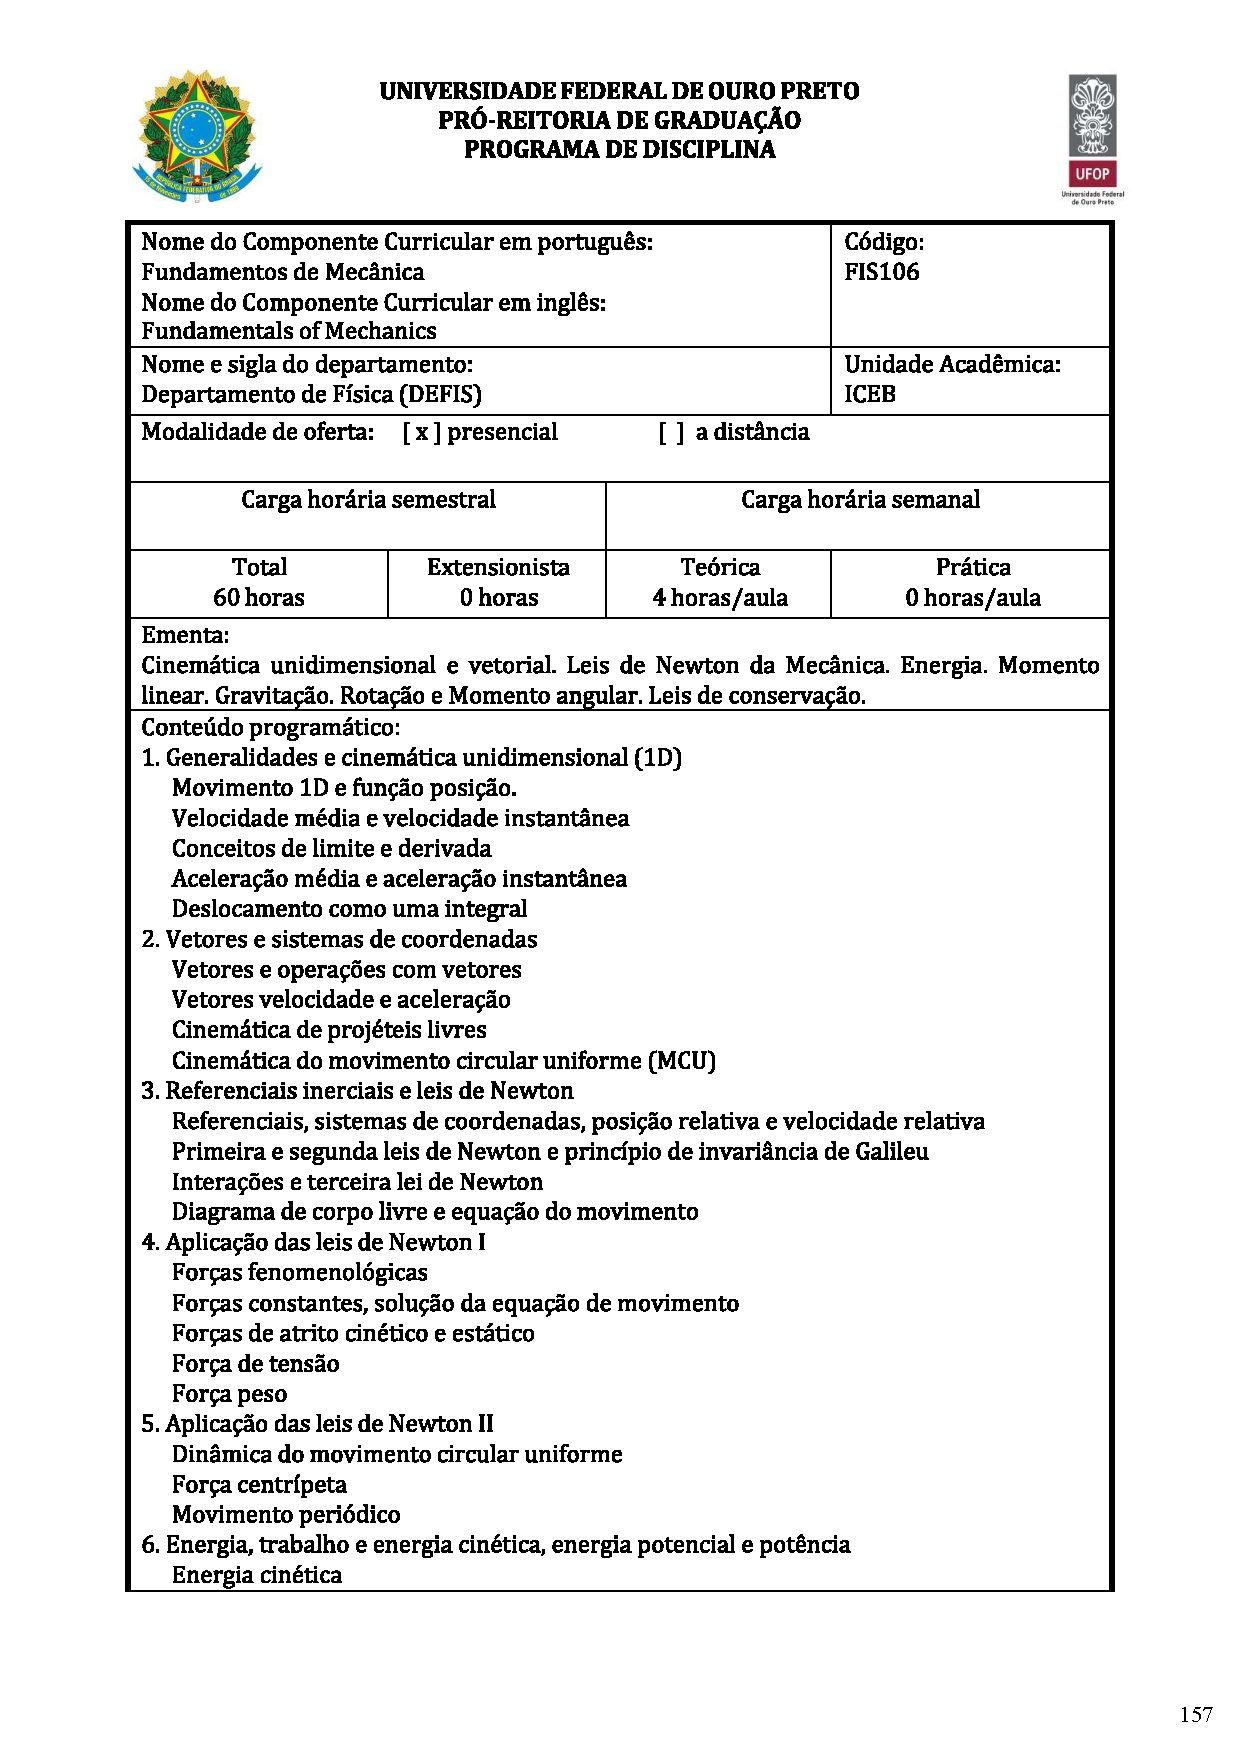
\includepdf[pages=-,nup=1x1, frame]{FIS106}
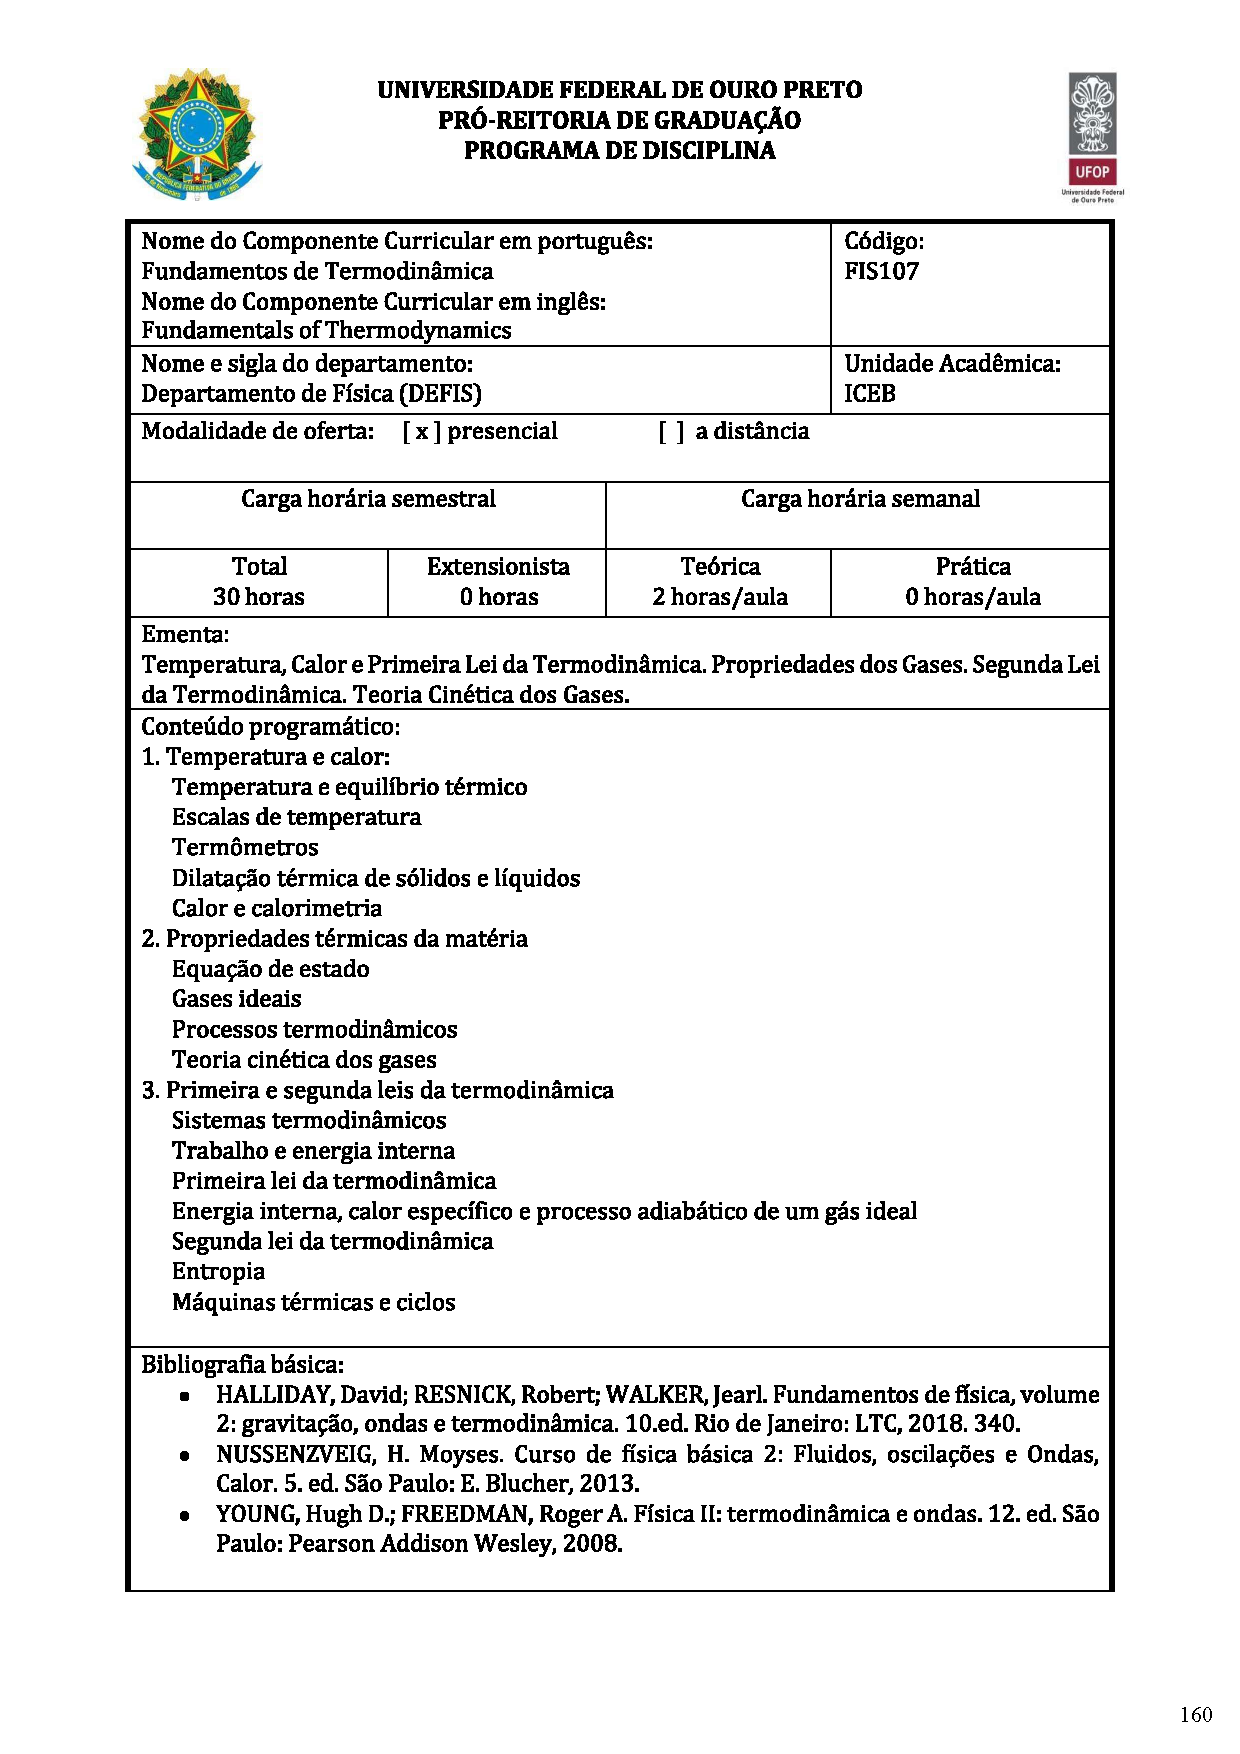
\includepdf[pages=-,nup=1x1, frame]{FIS107}
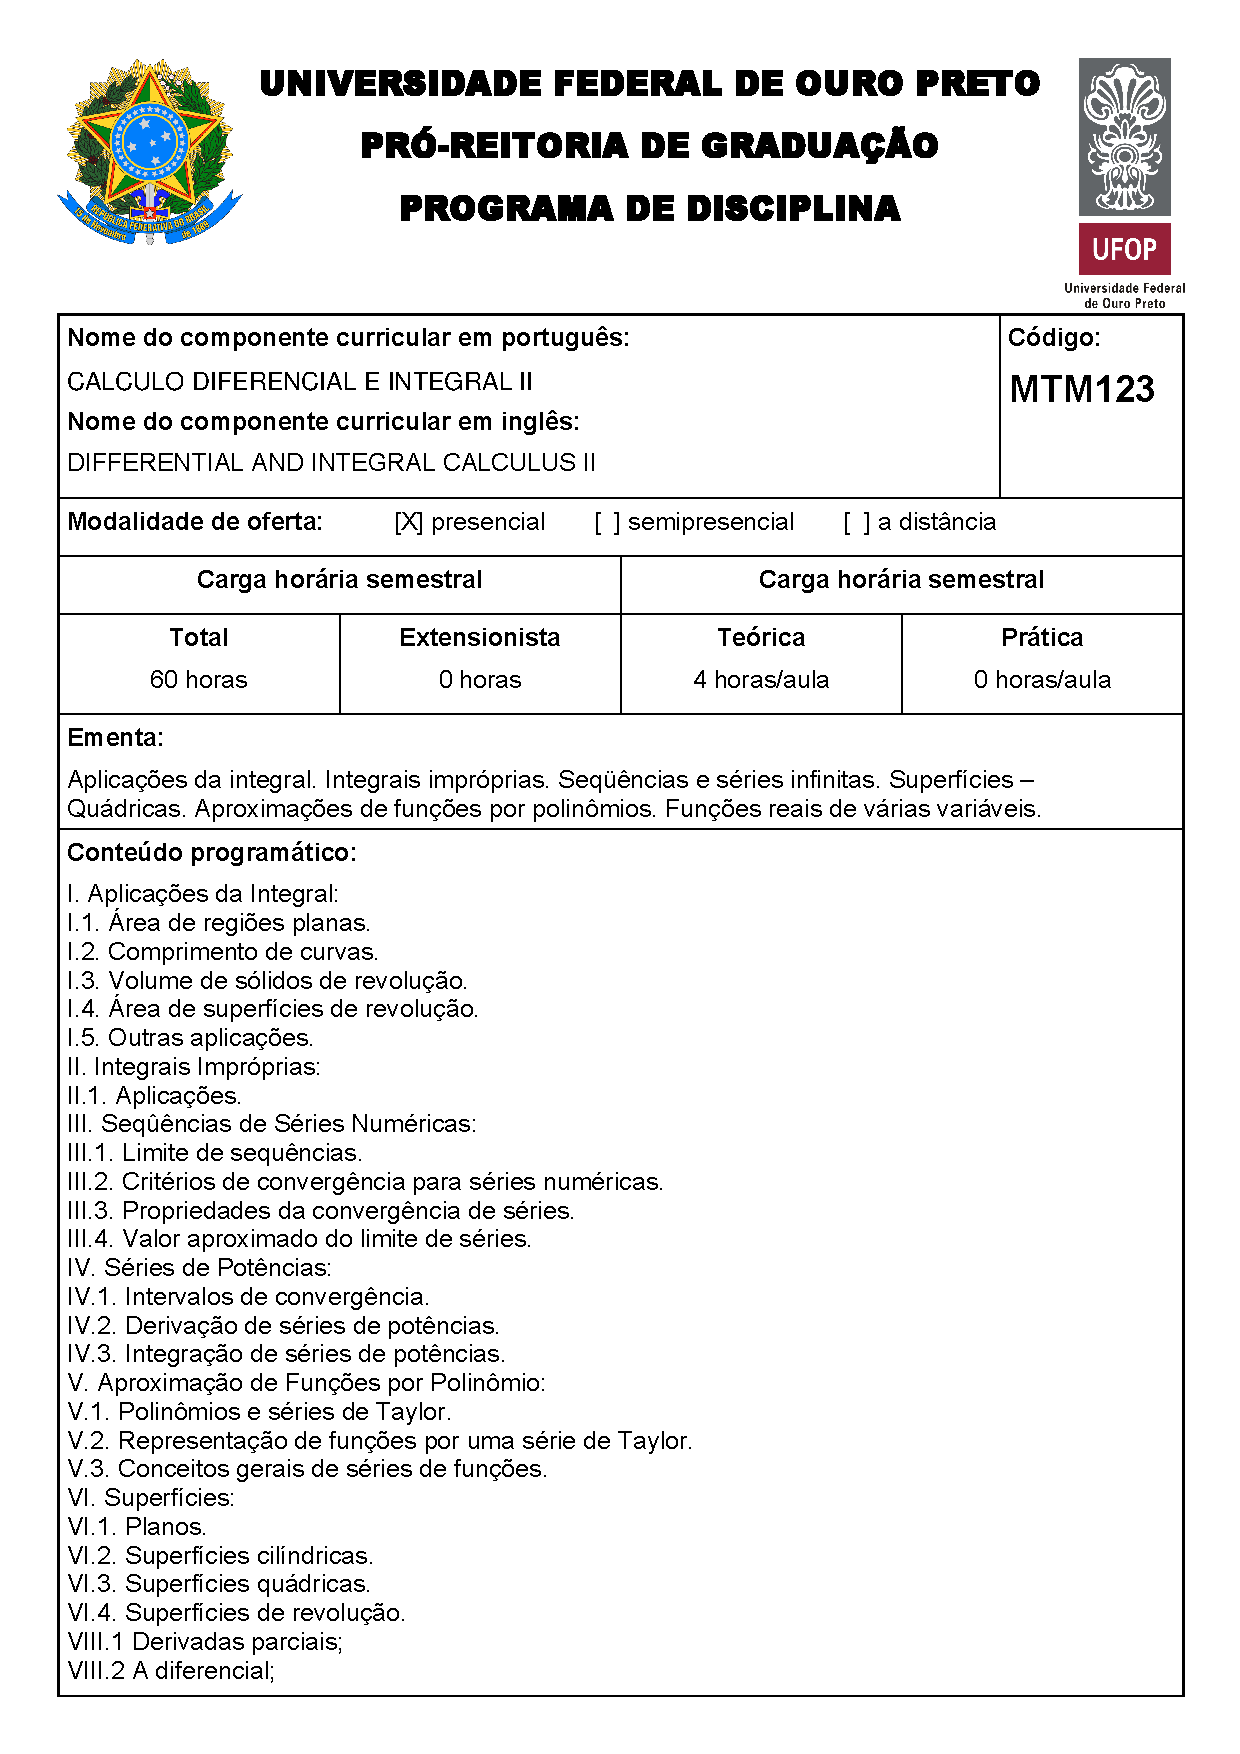
\includepdf[pages=-,nup=1x1, frame]{MTM123}
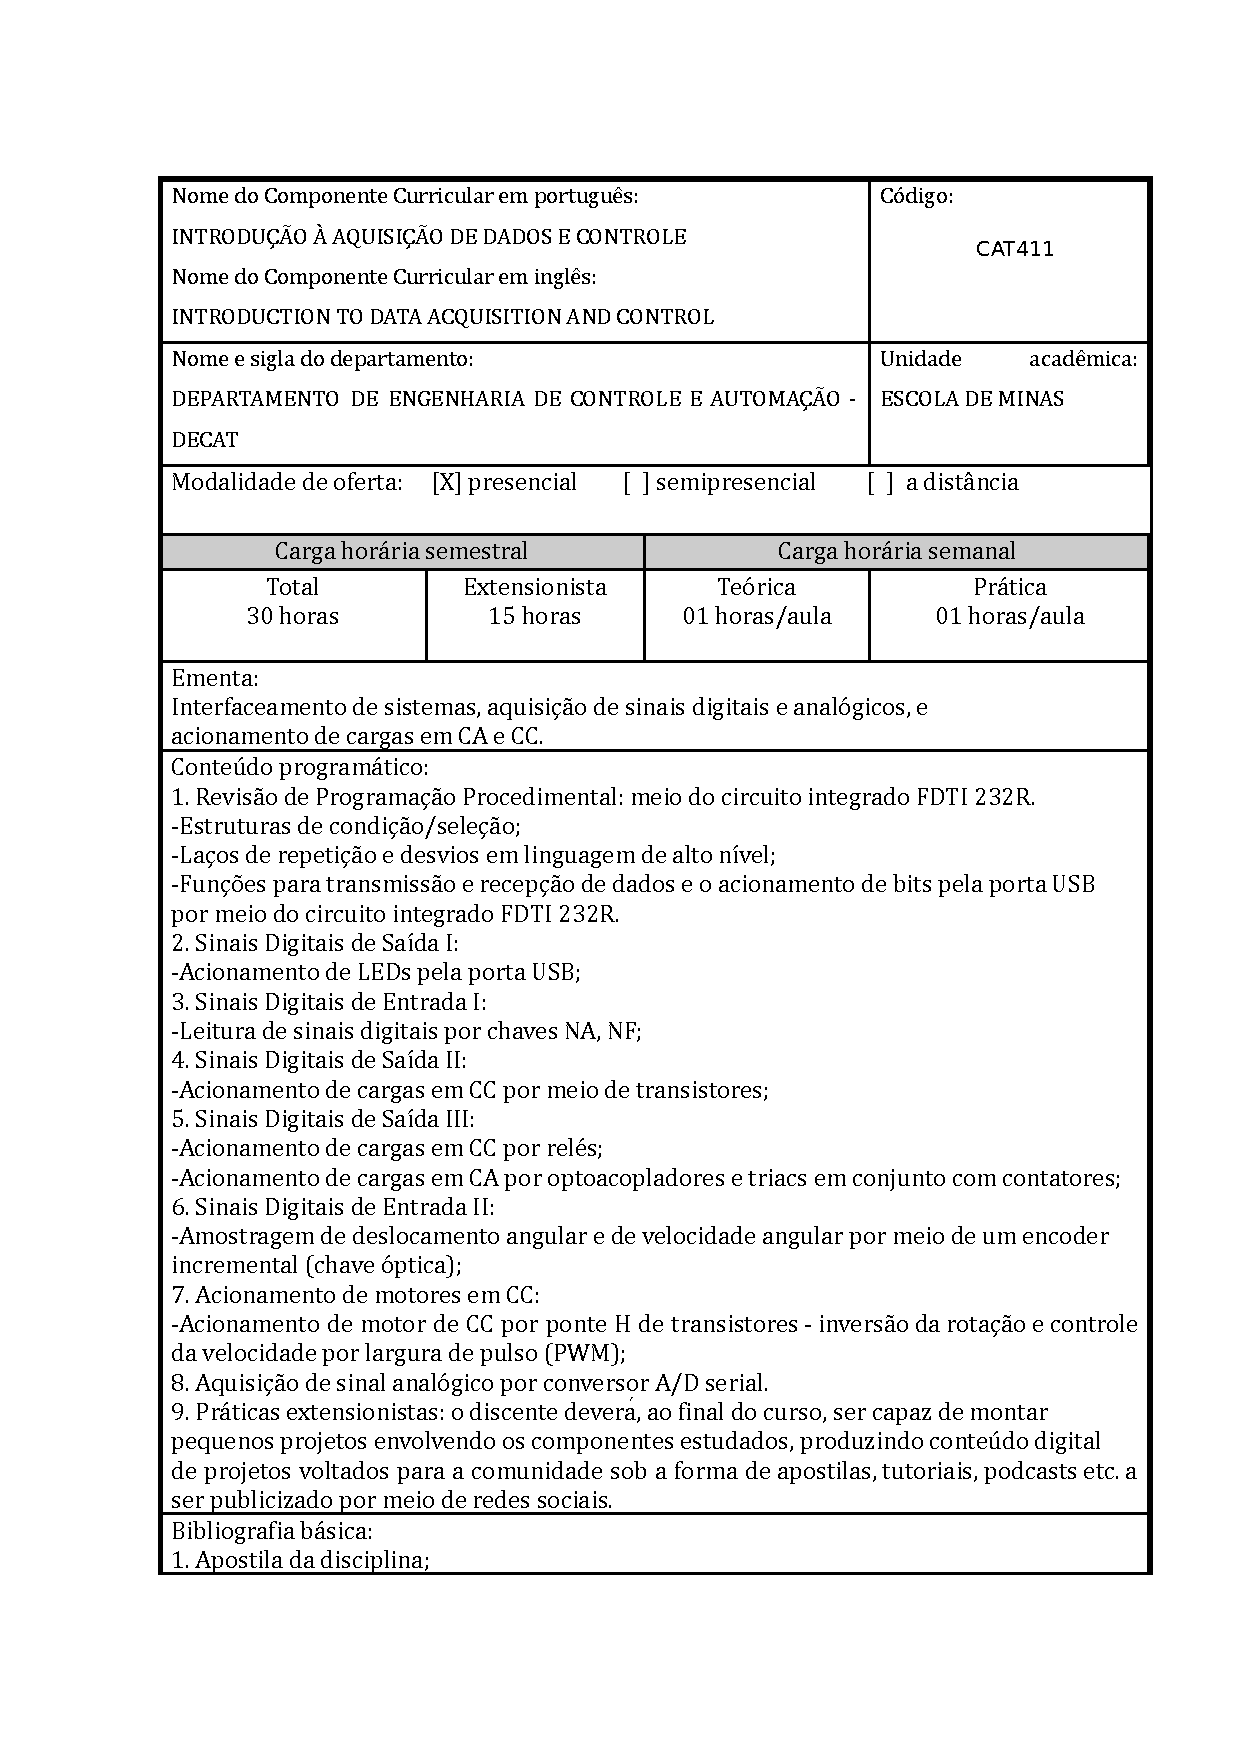
\includepdf[pages=-,nup=1x1, frame]{CAT411} % CAT002
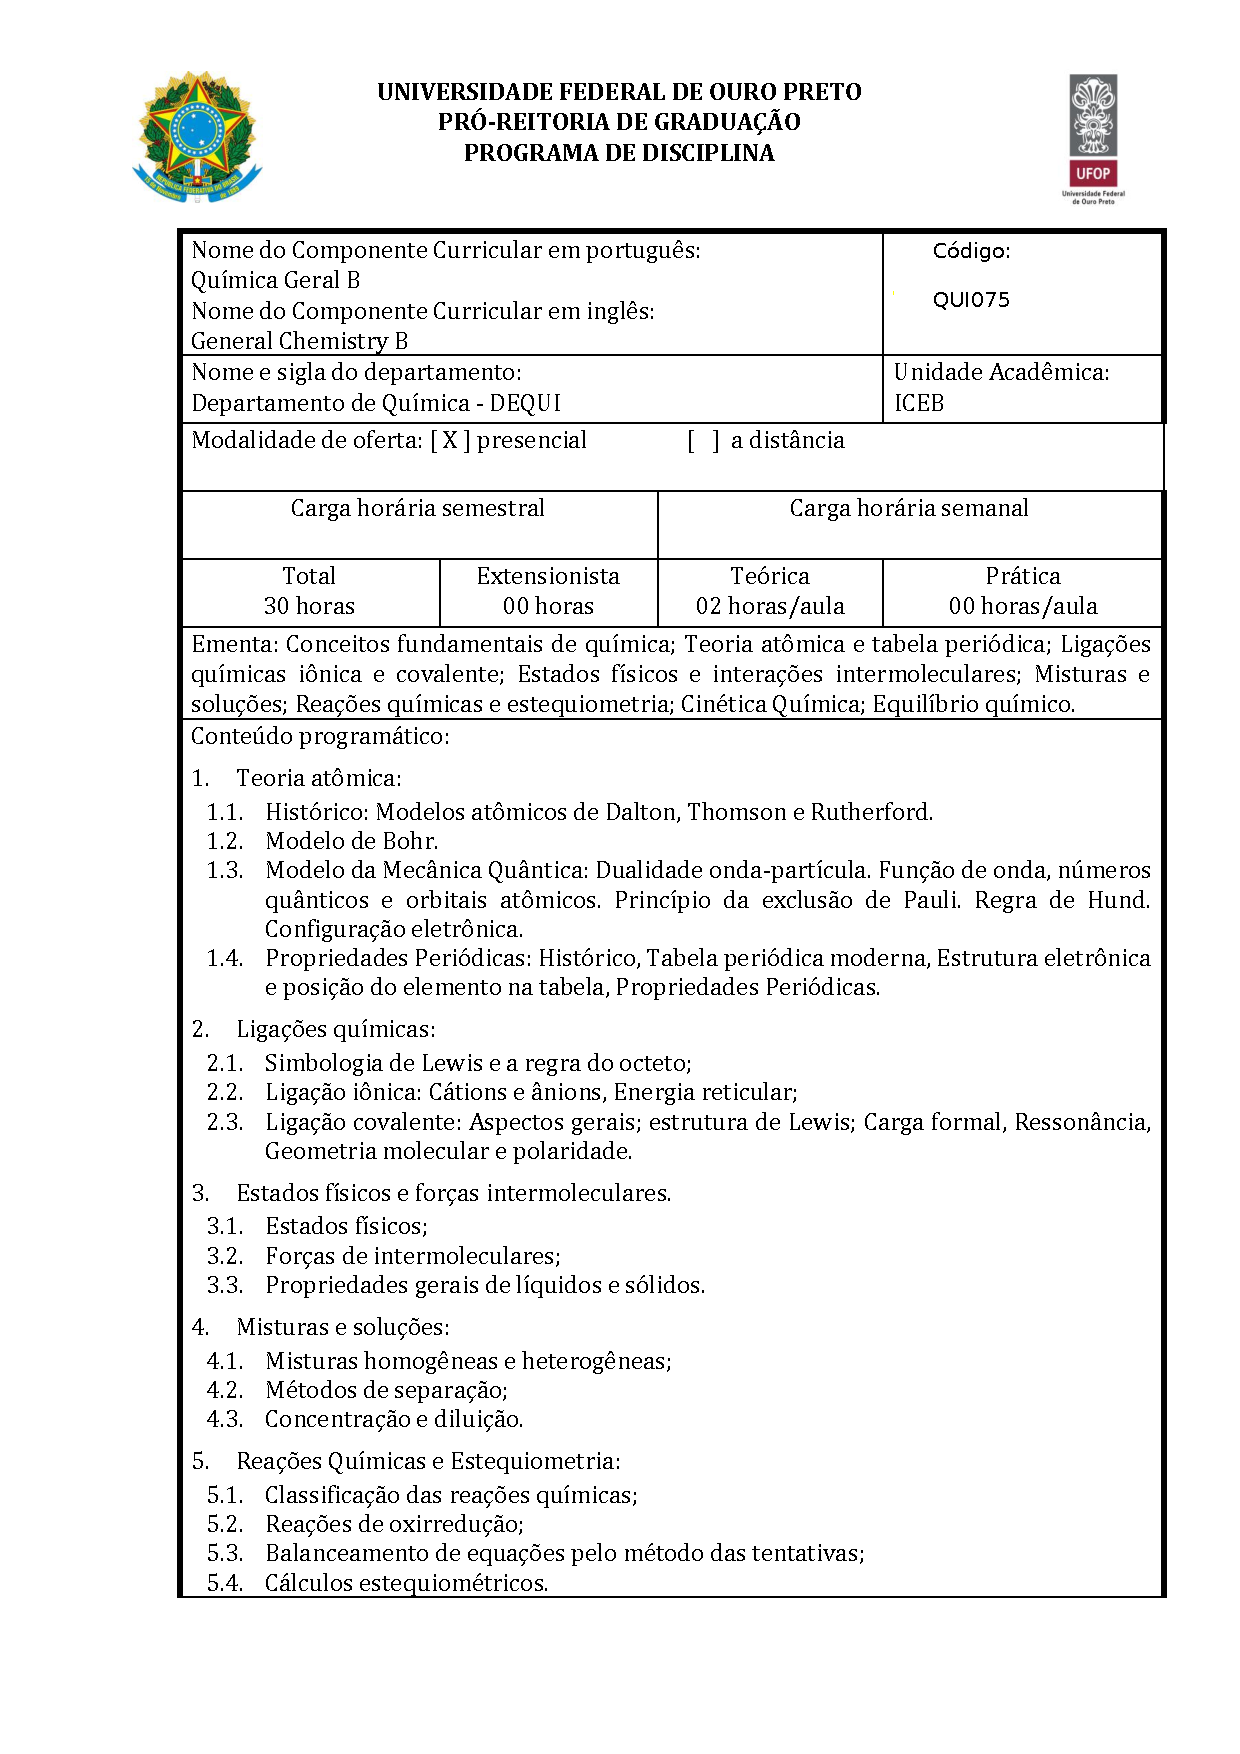
\includepdf[pages=-,nup=1x1, frame]{QUI075} % QUIXXB
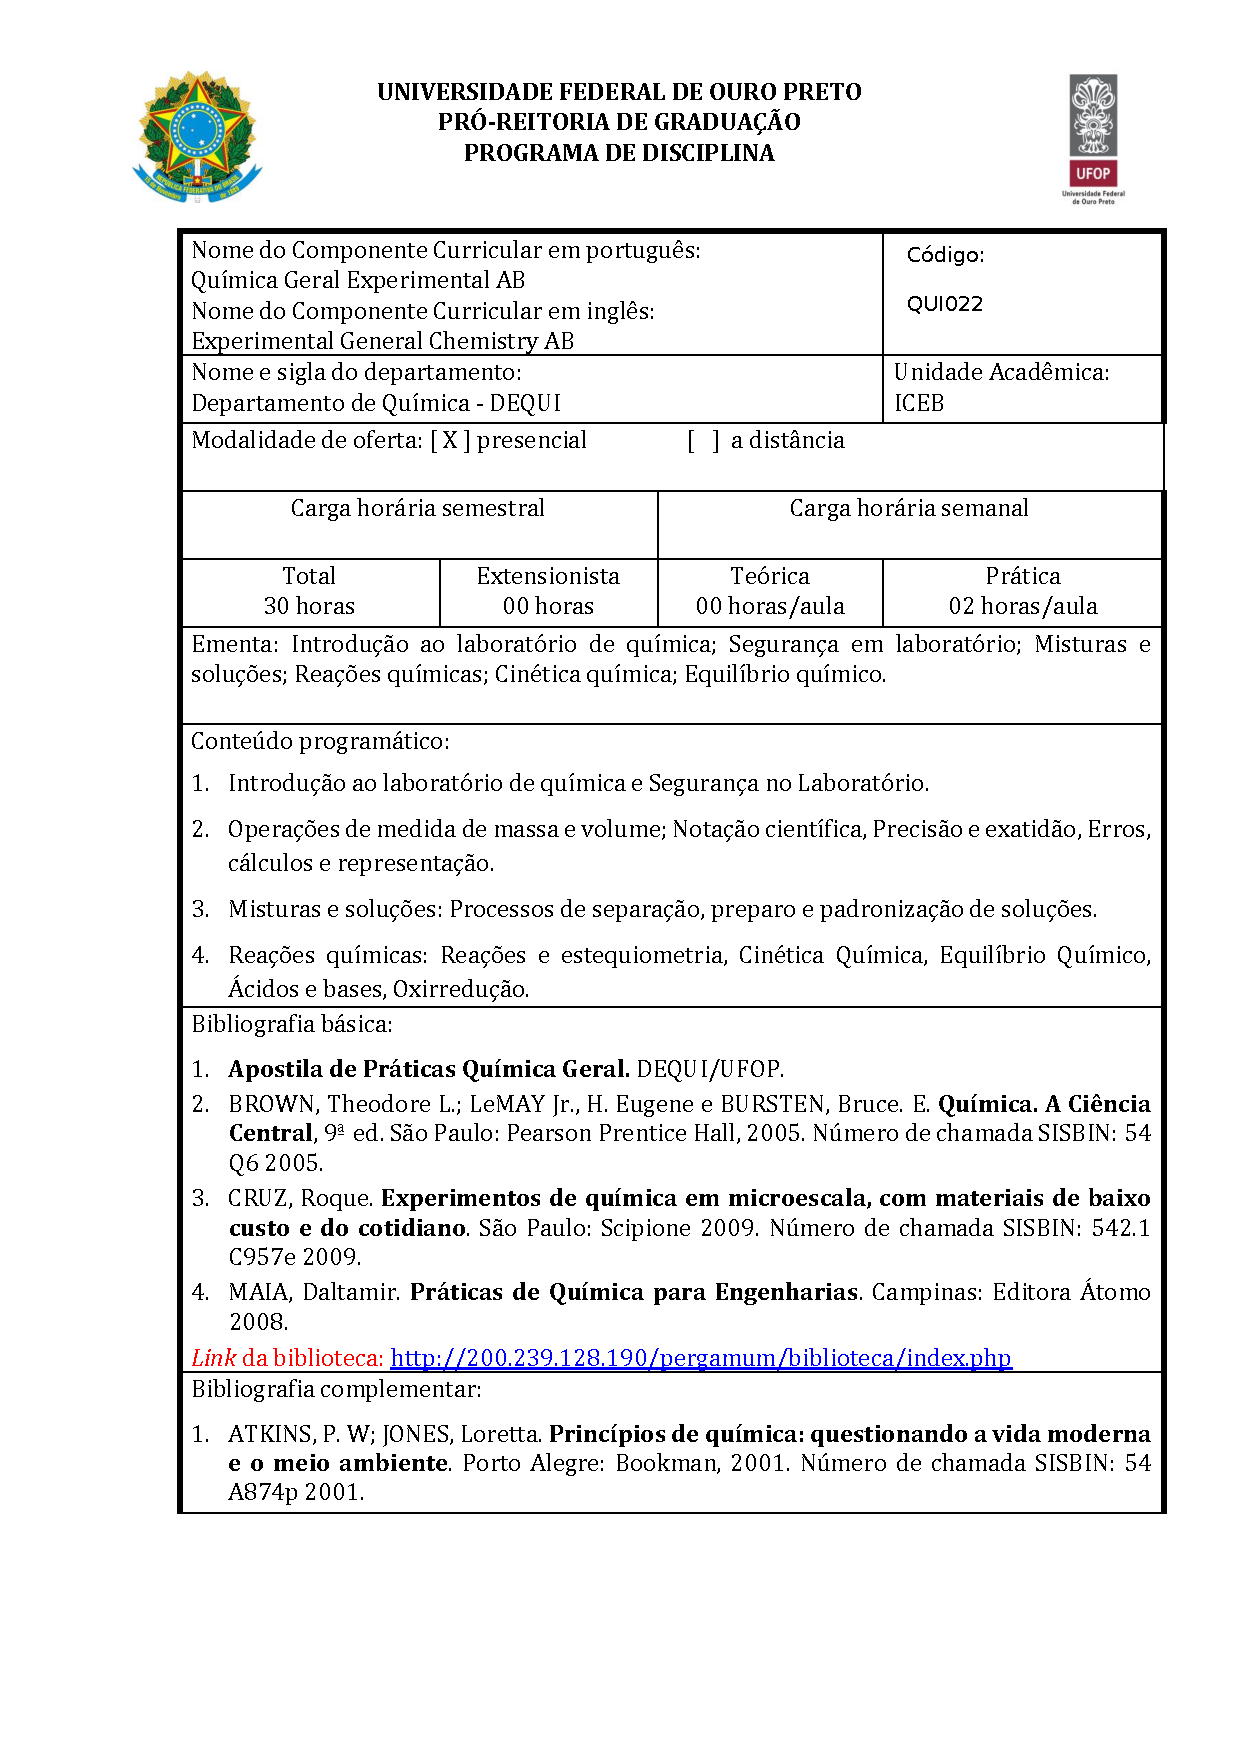
\includepdf[pages=-,nup=1x1, frame]{QUI022} % QUIXAB


% terceiro semestre
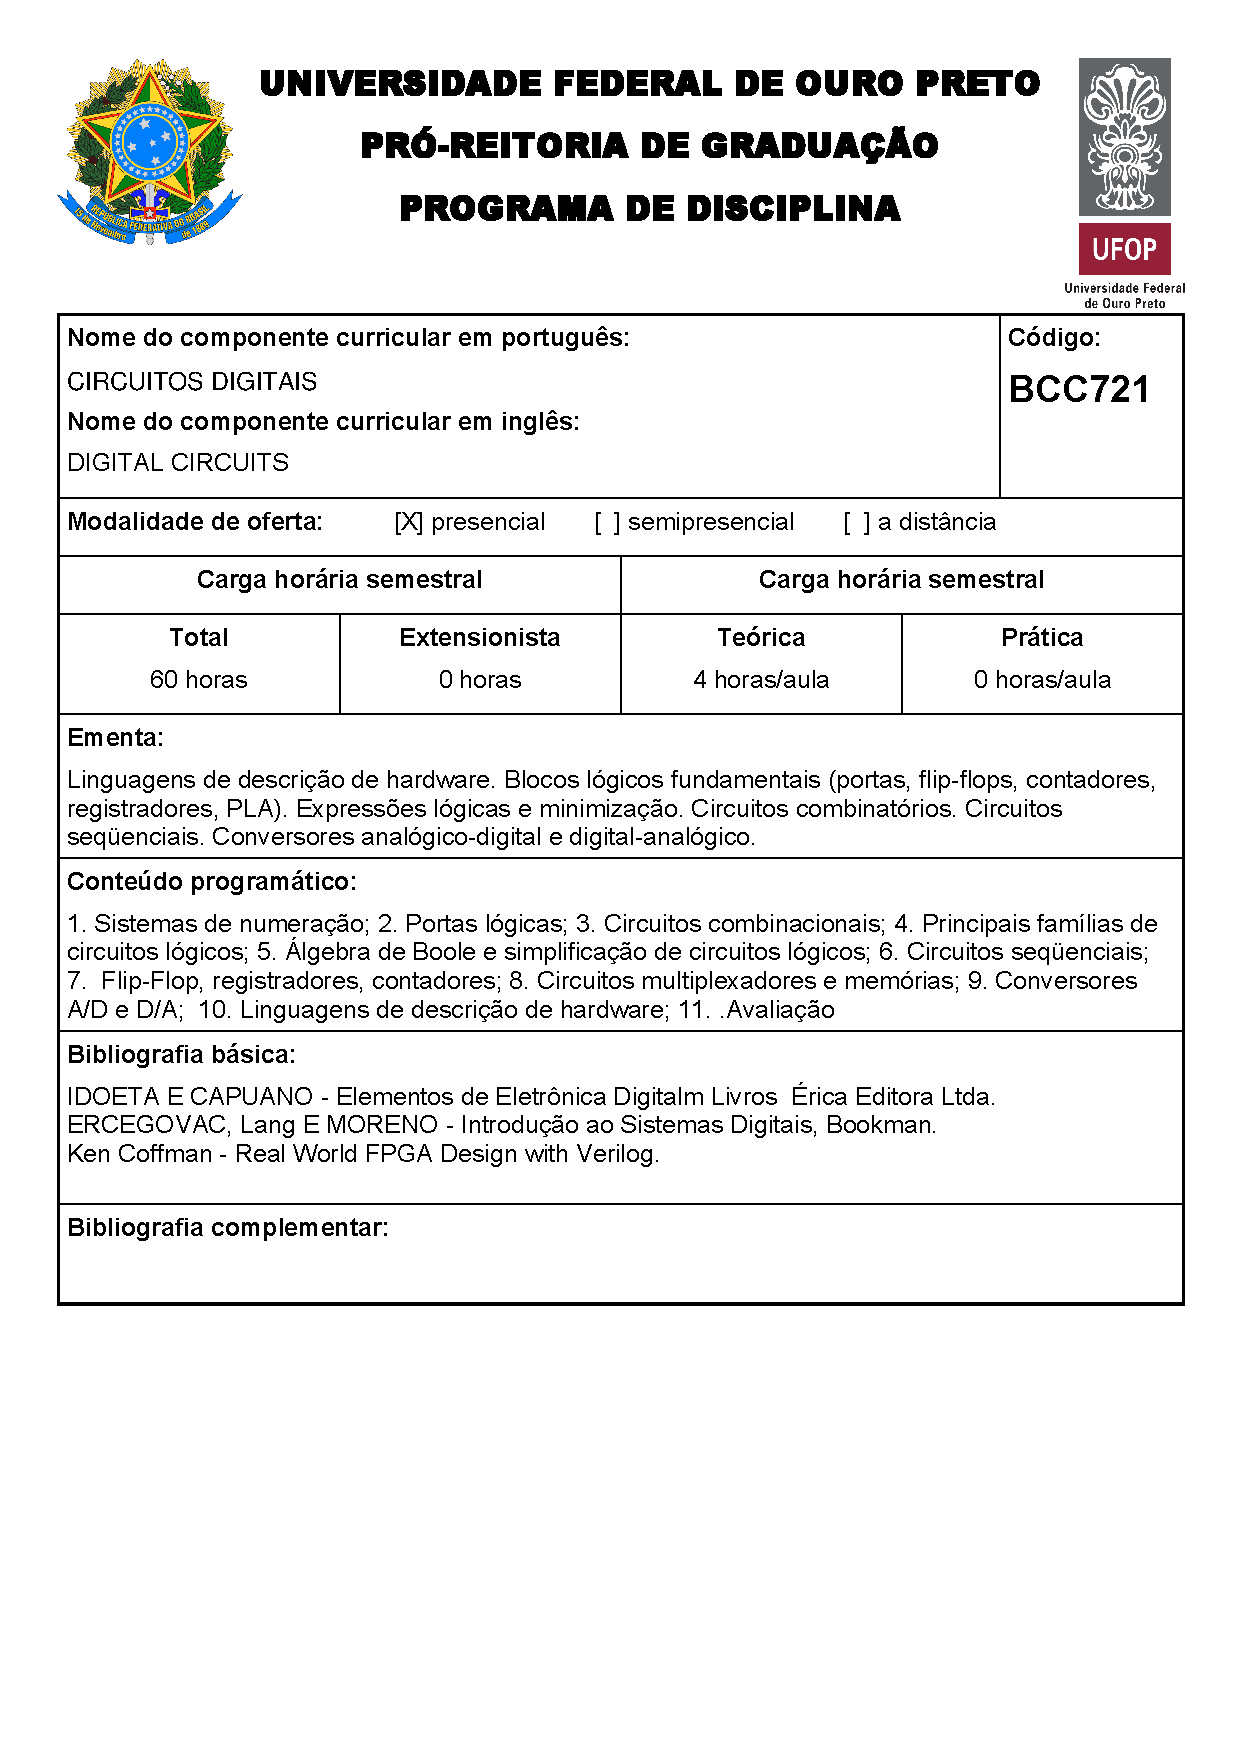
\includepdf[pages=-,nup=1x1, frame]{BCC721}
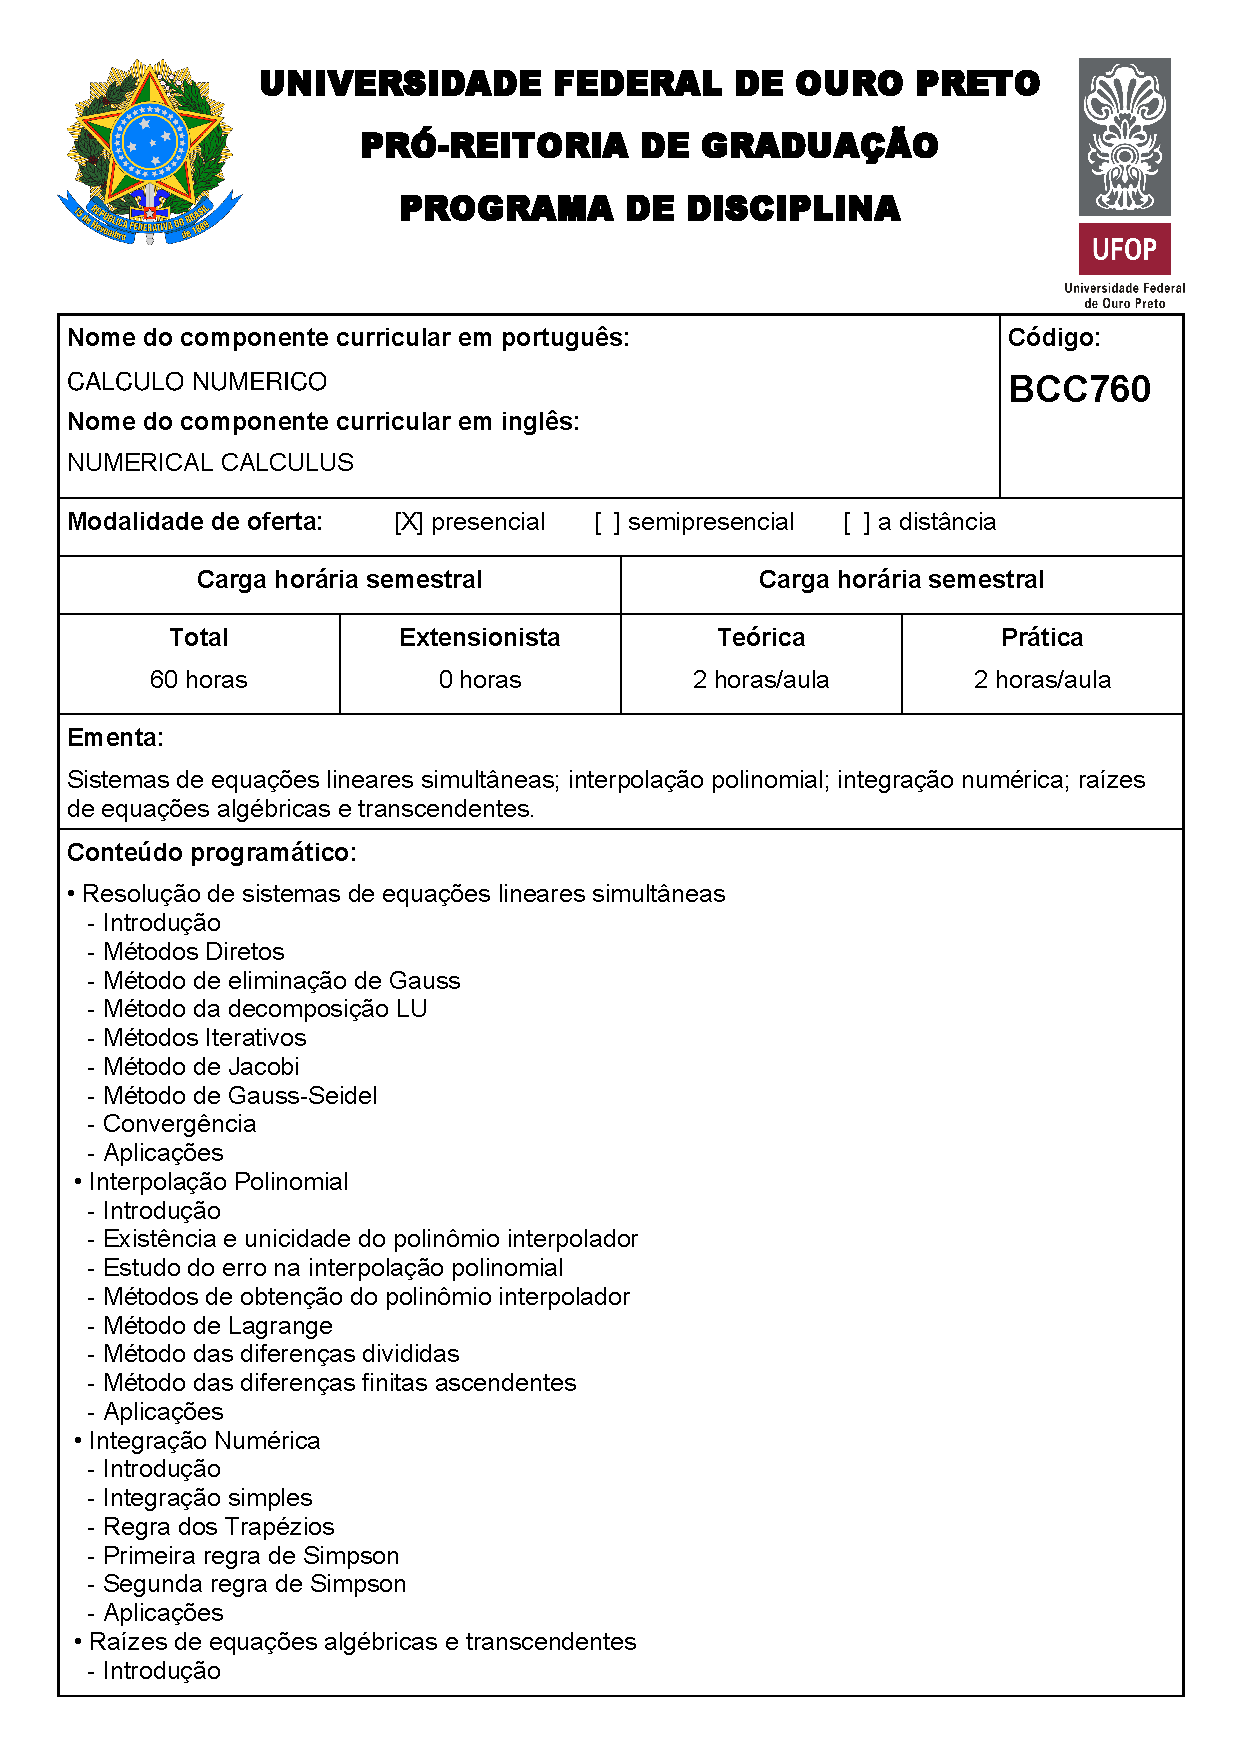
\includepdf[pages=-,nup=1x1, frame]{BCC760}
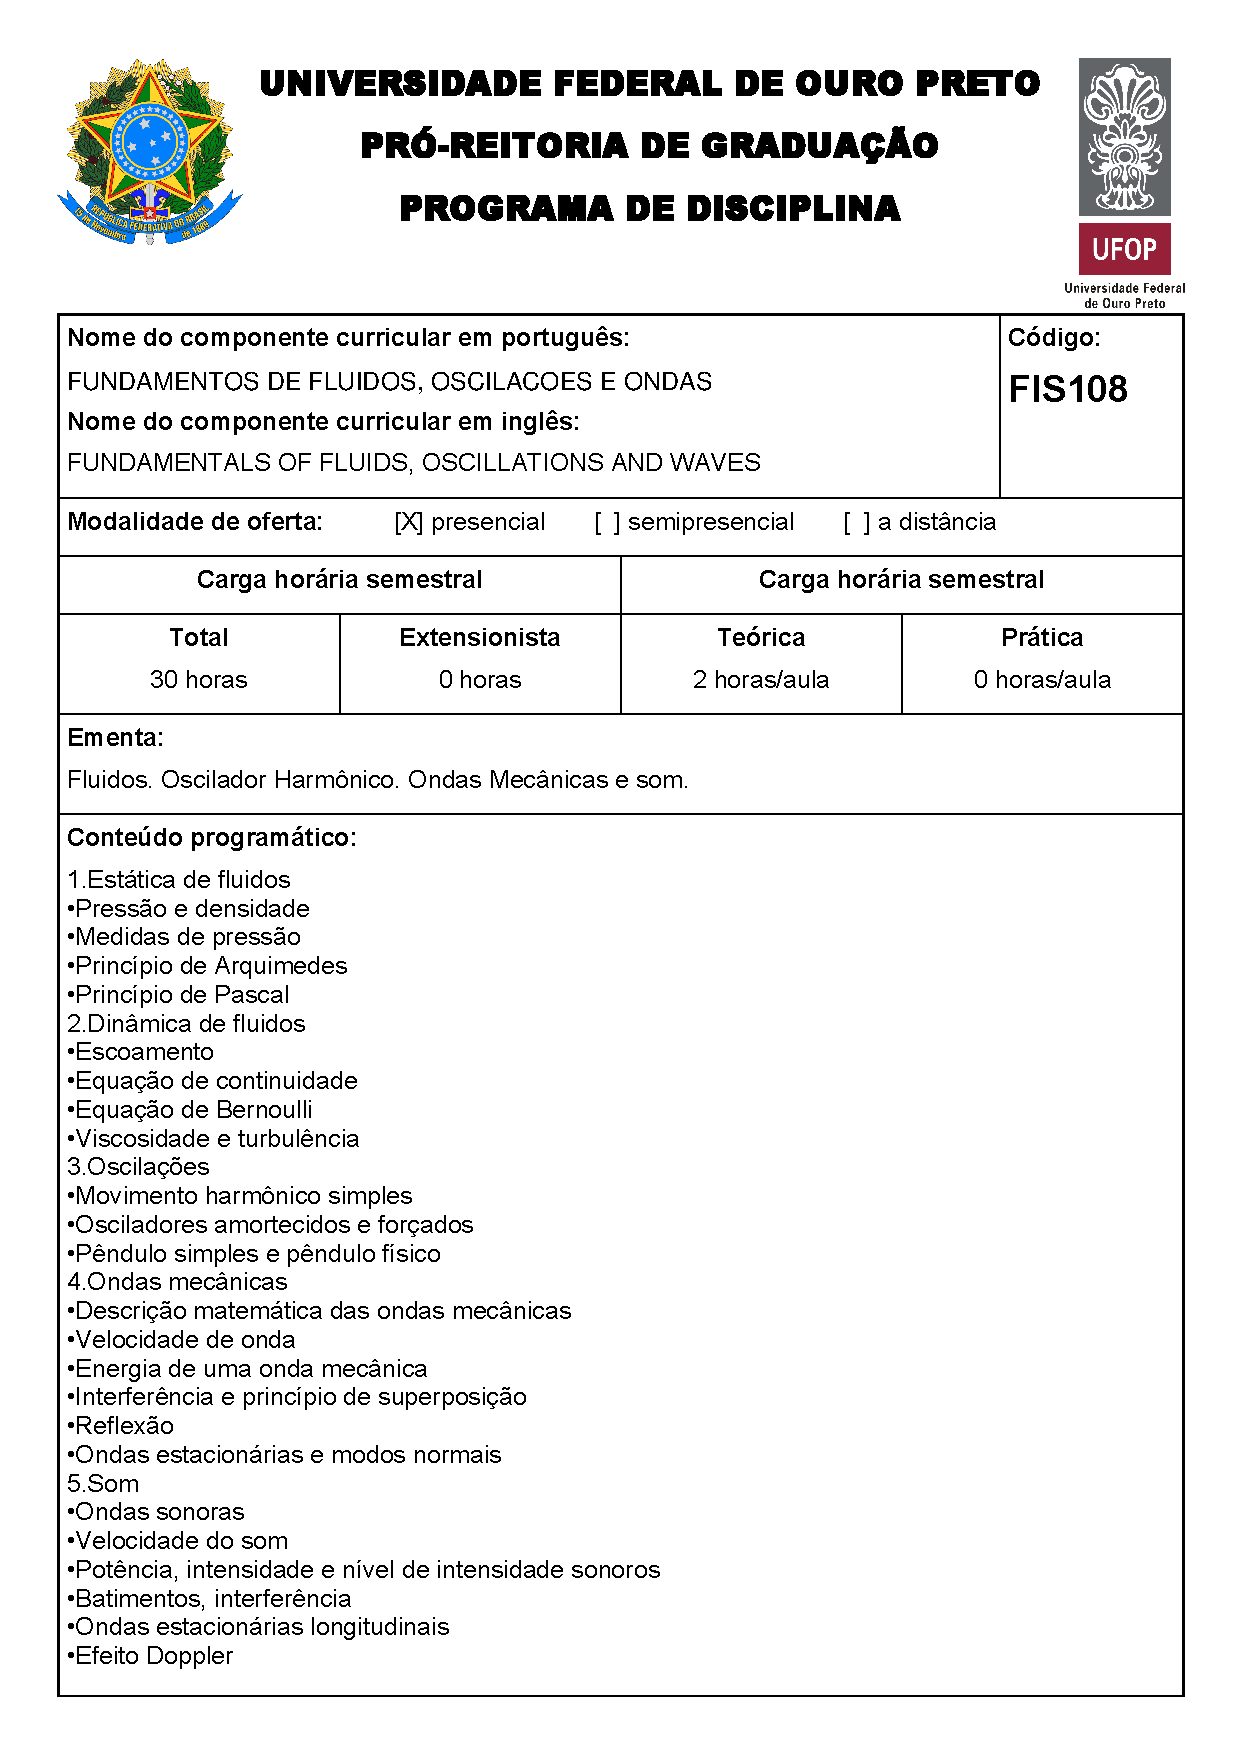
\includepdf[pages=-,nup=1x1, frame]{FIS108}
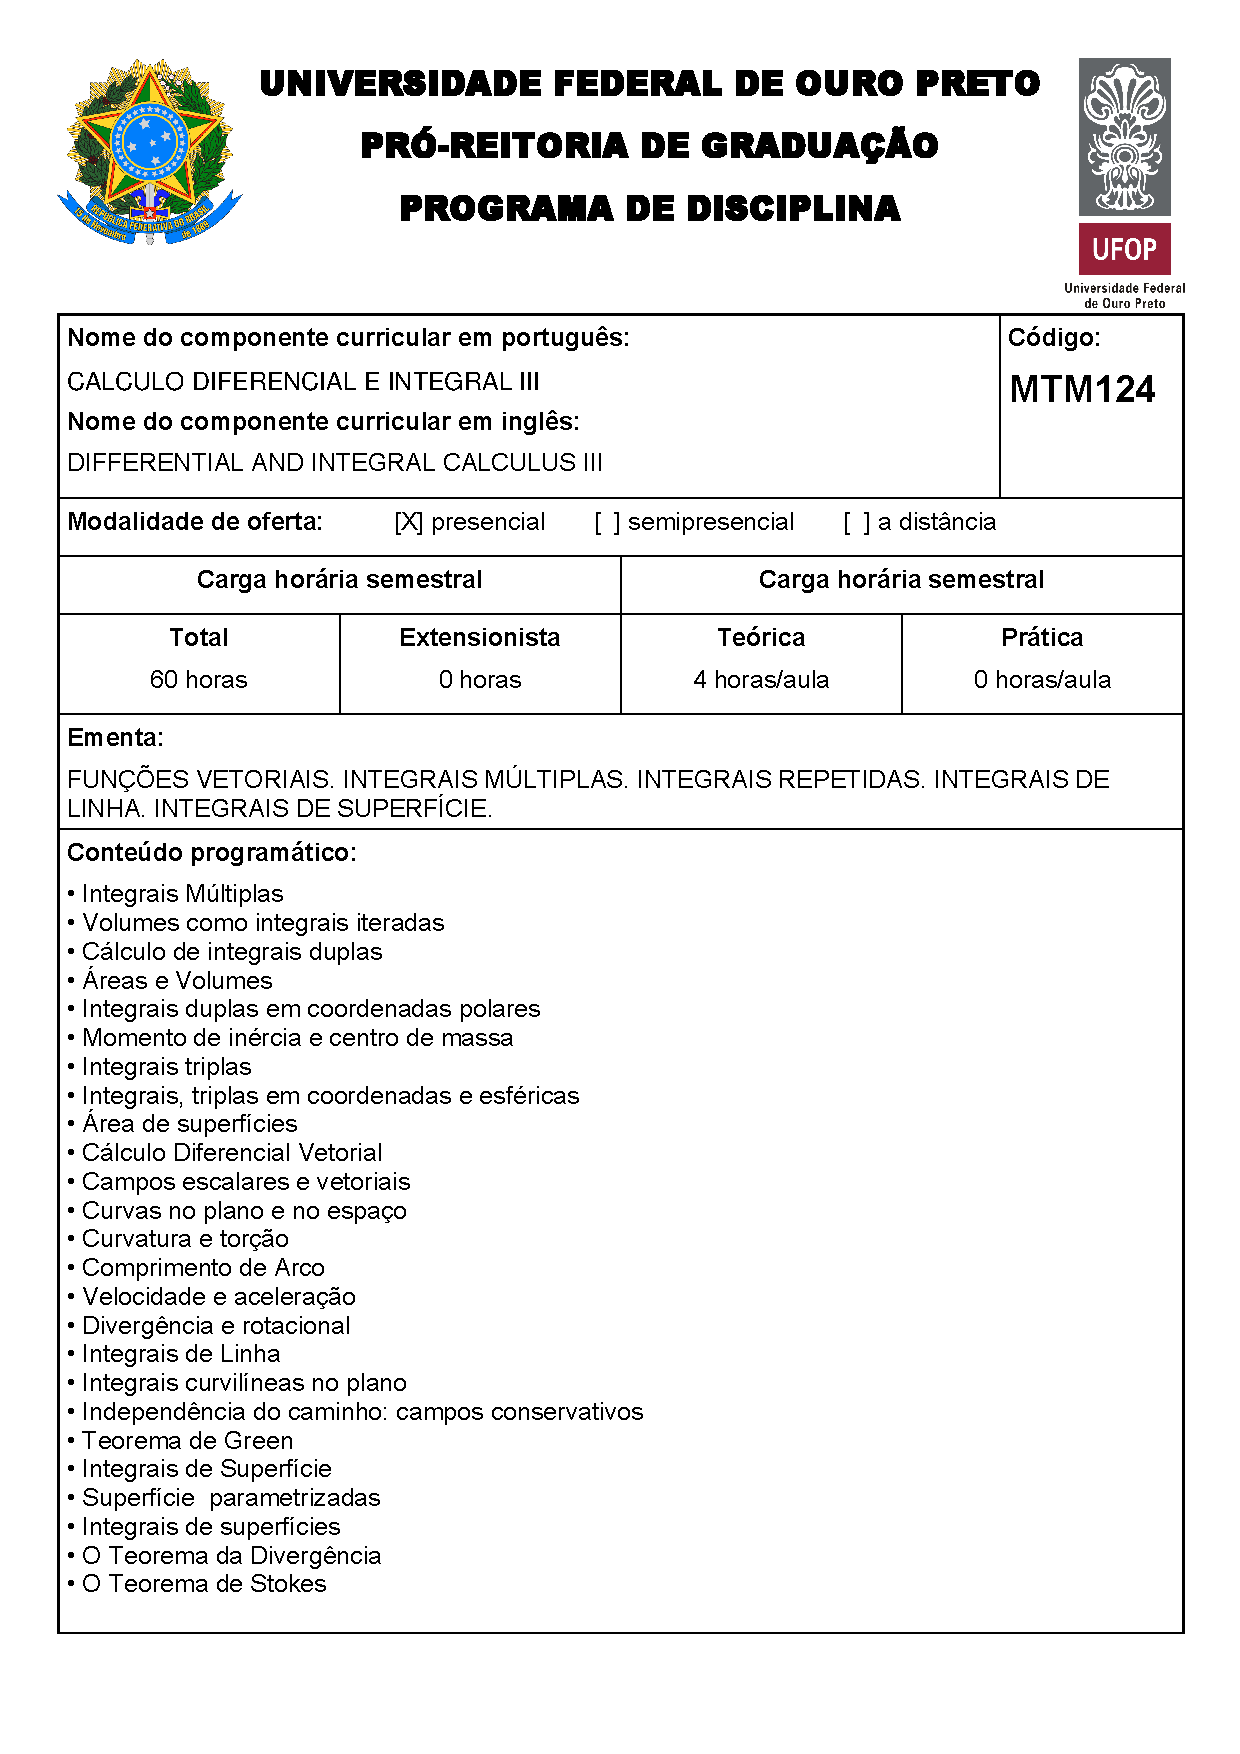
\includepdf[pages=-,nup=1x1, frame]{MTM124}
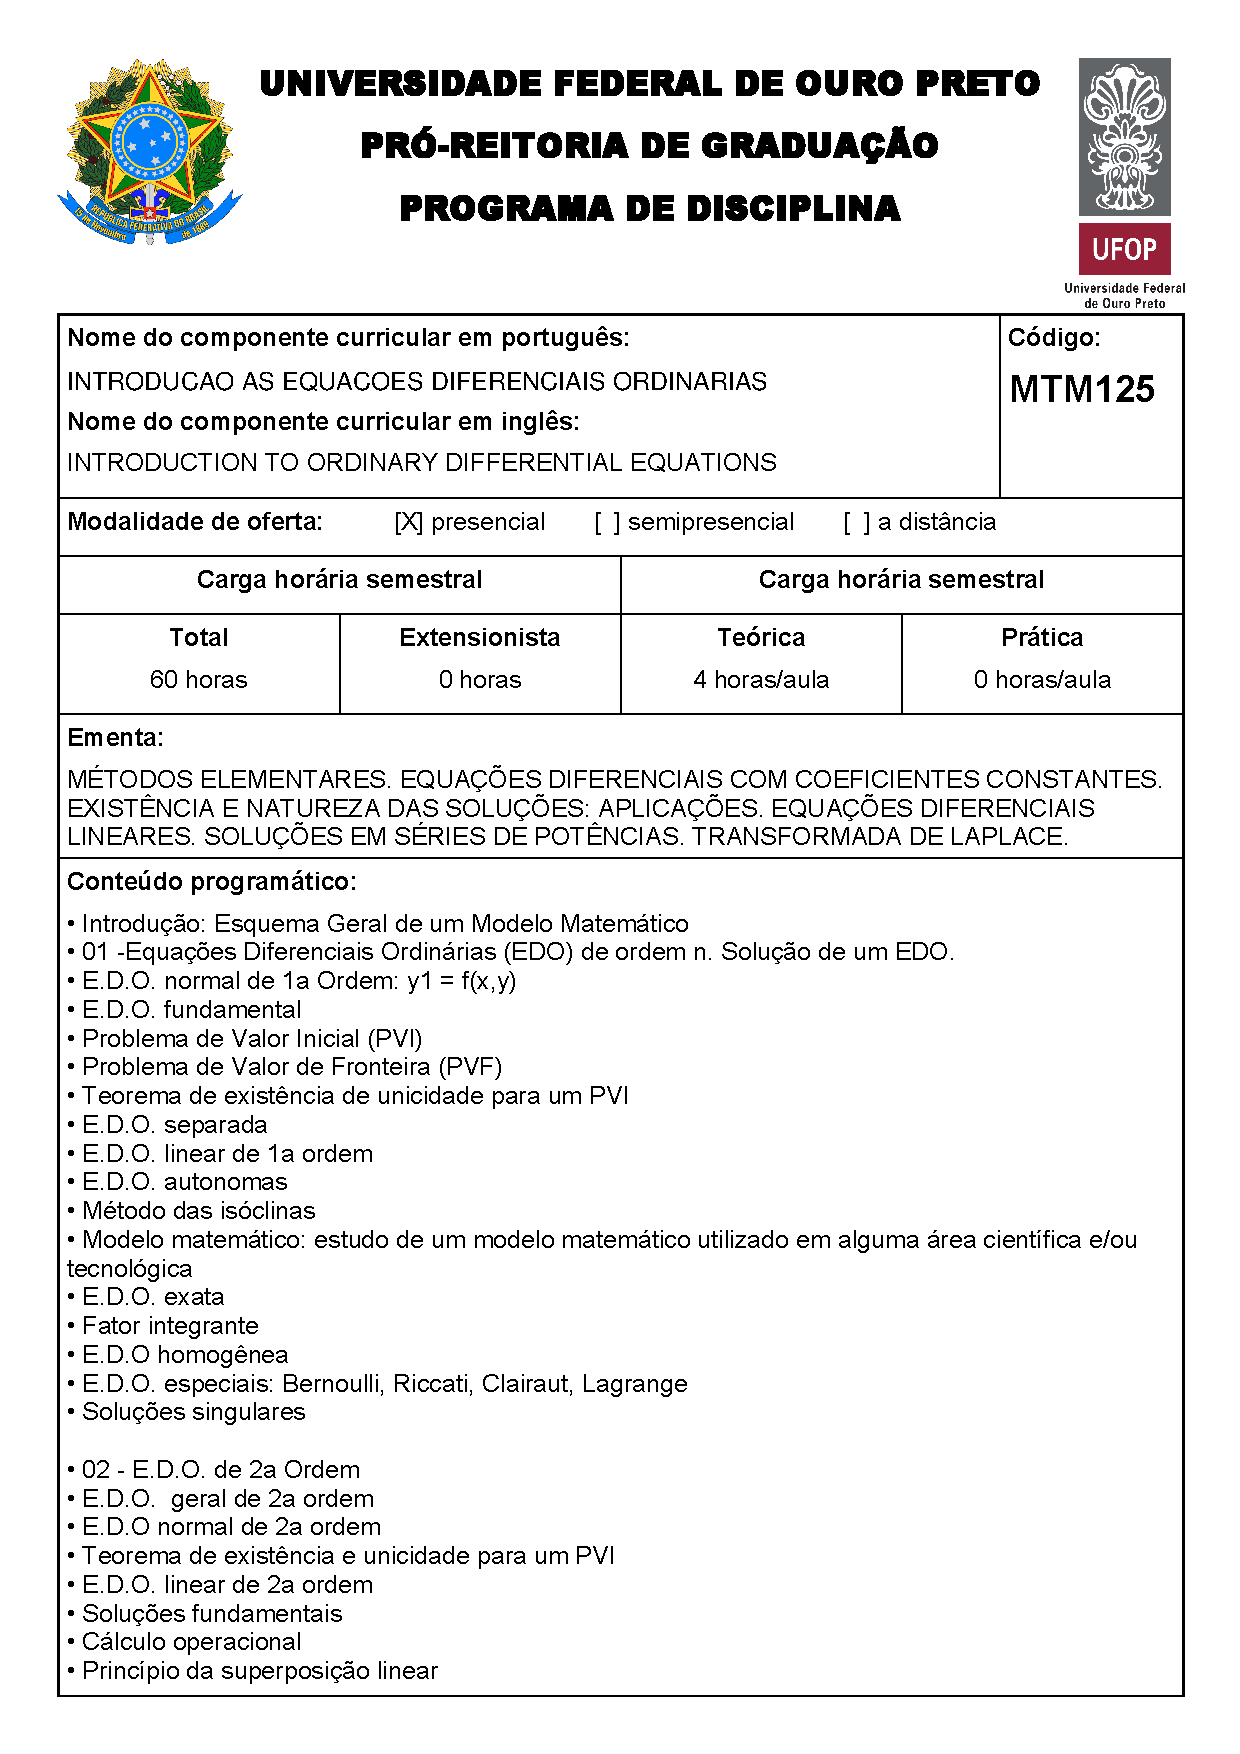
\includepdf[pages=-,nup=1x1, frame]{MTM125}
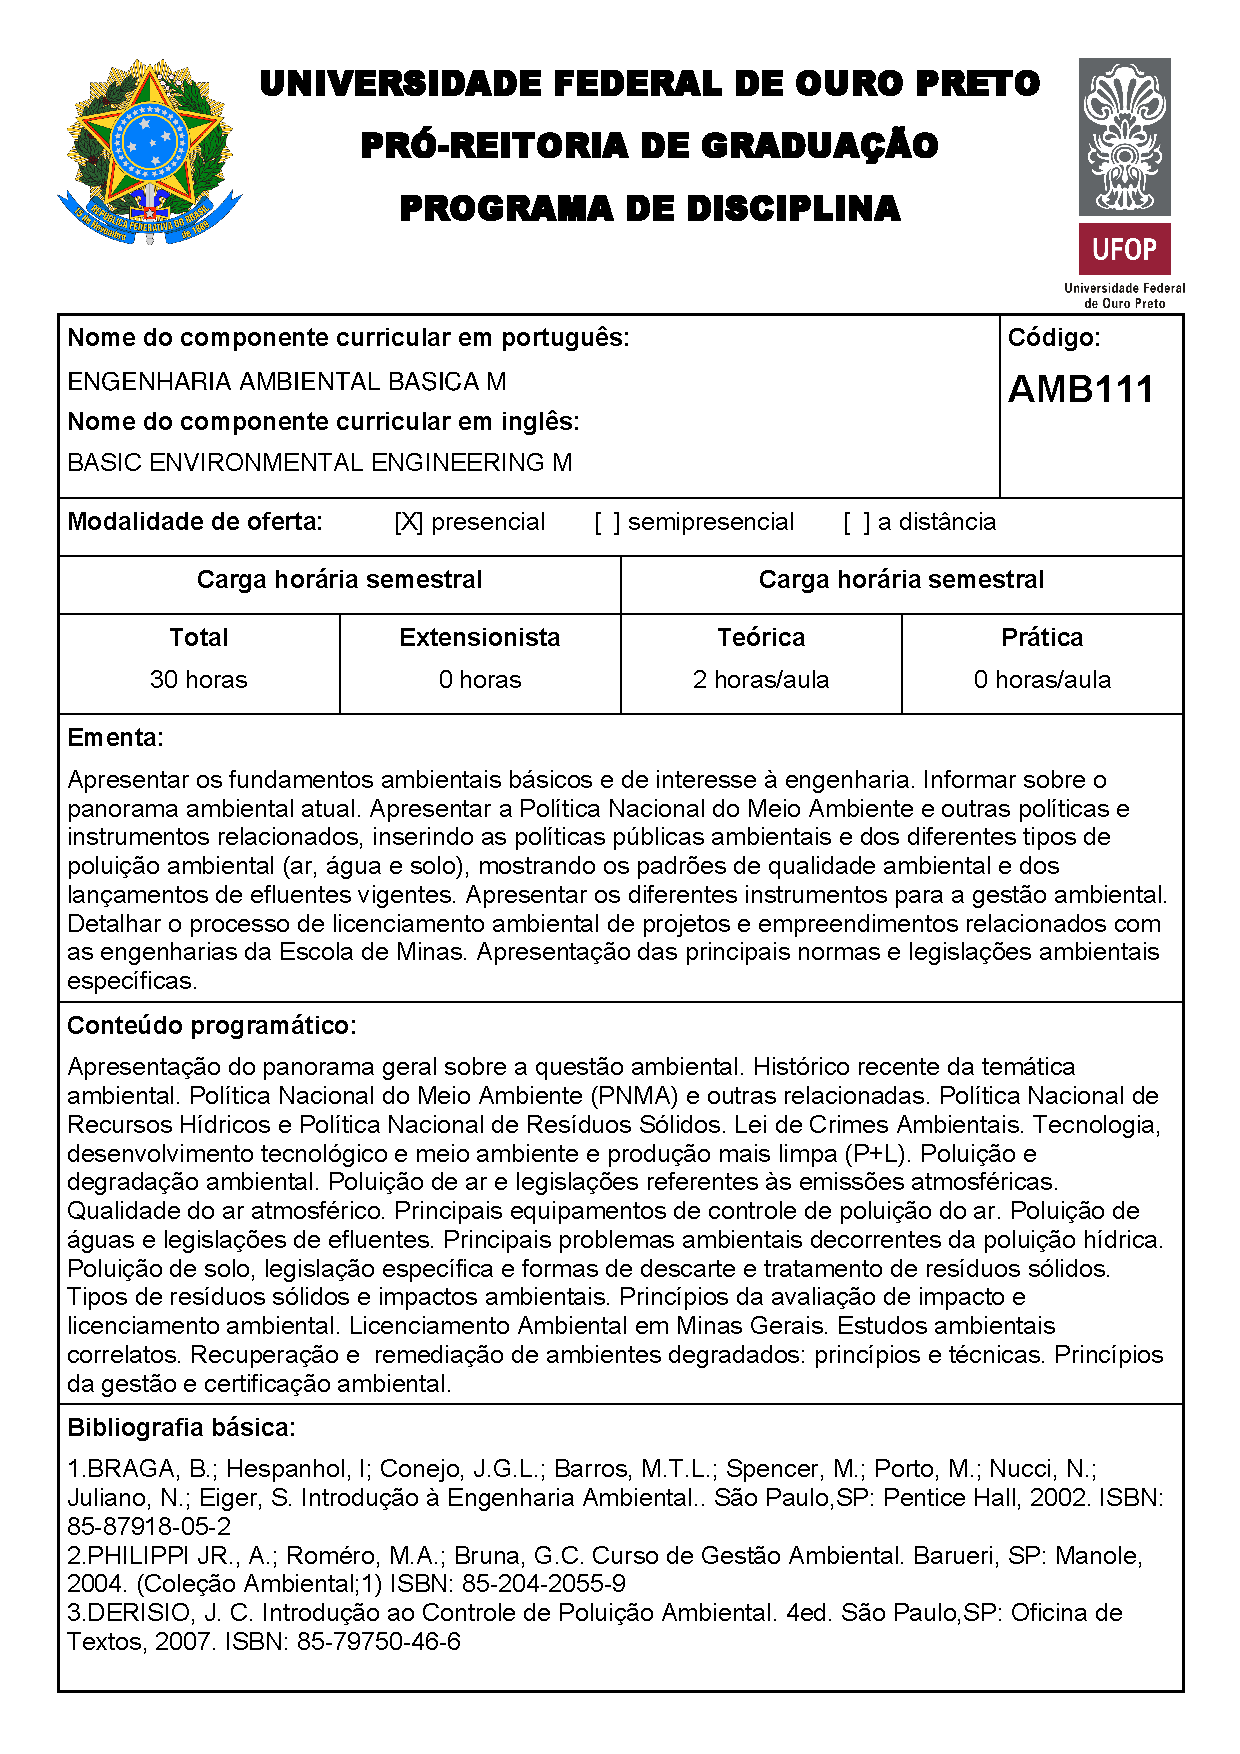
\includepdf[pages=-,nup=1x1, frame]{AMB111}


% quarto semestre
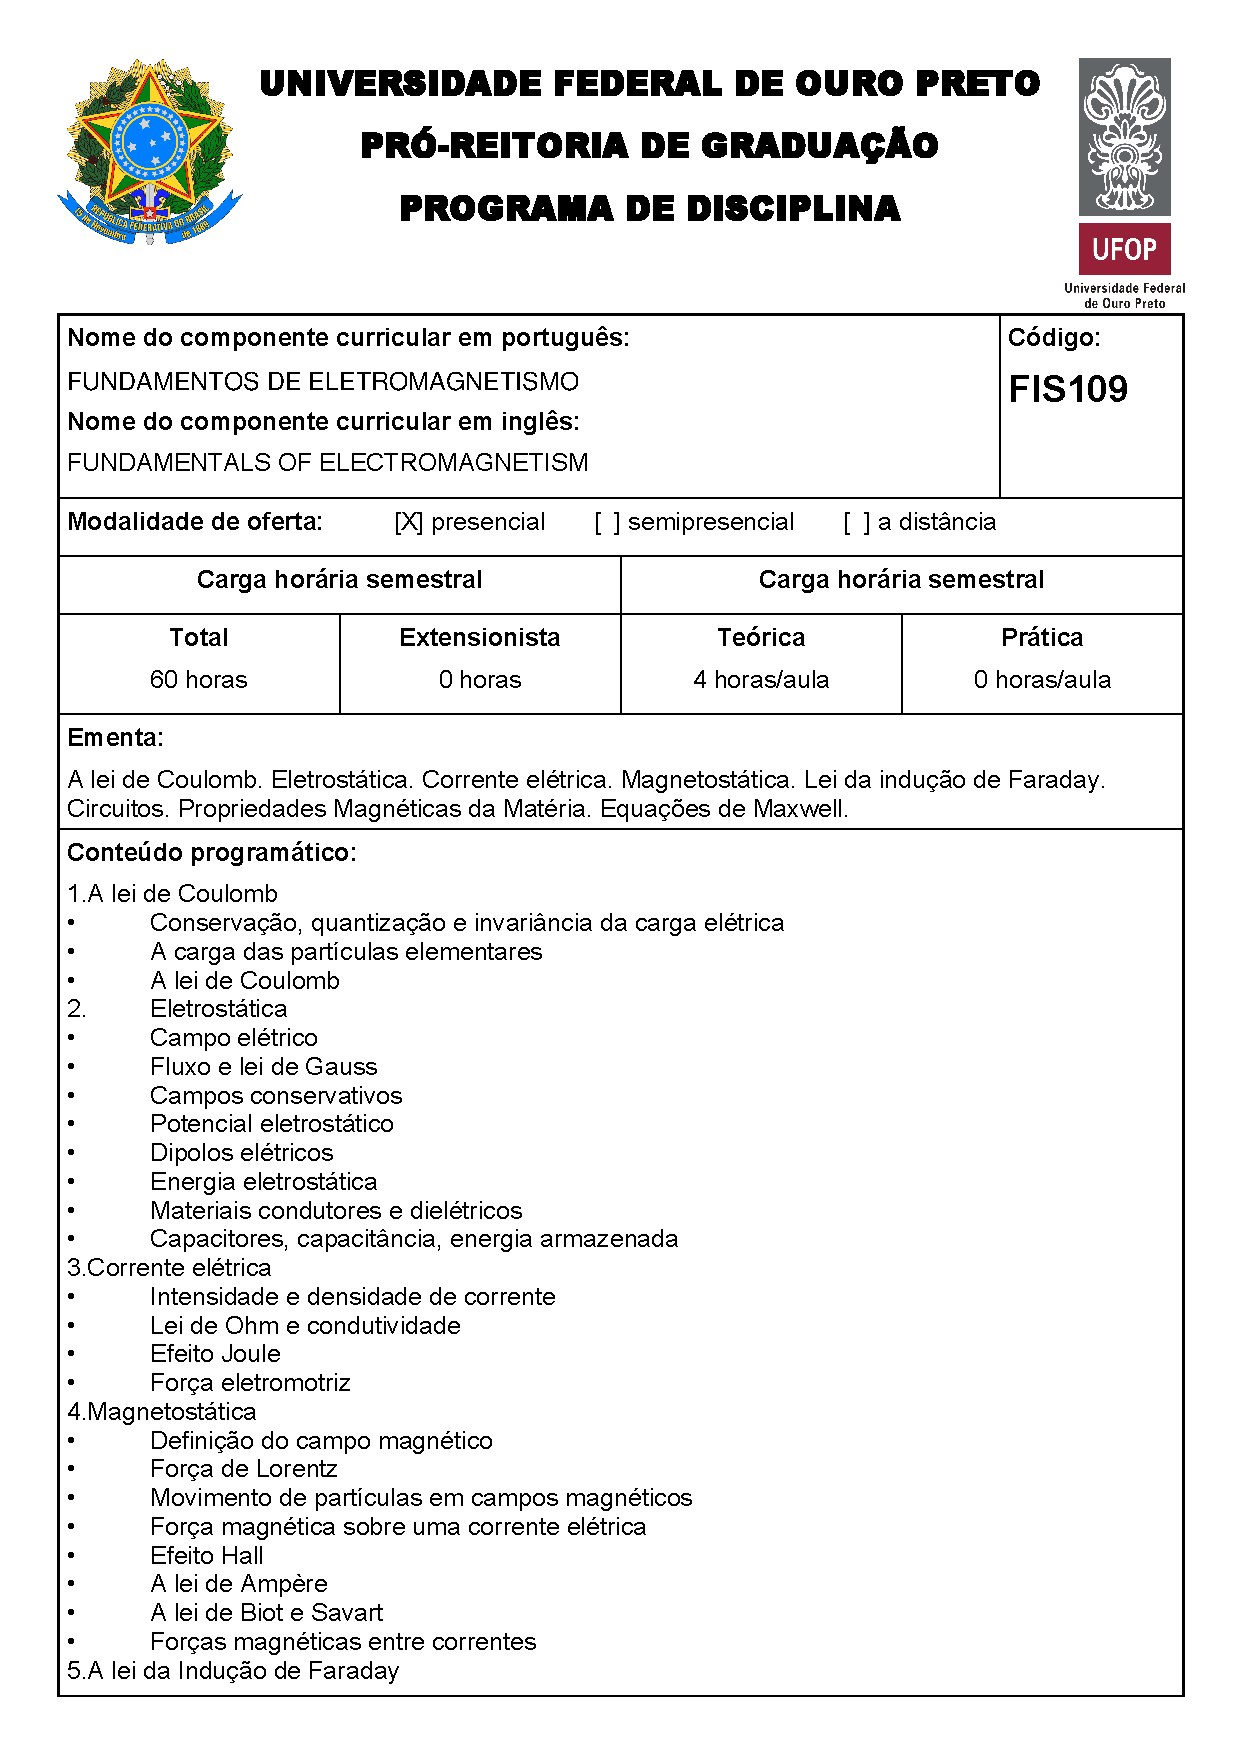
\includepdf[pages=-,nup=1x1, frame]{FIS109}
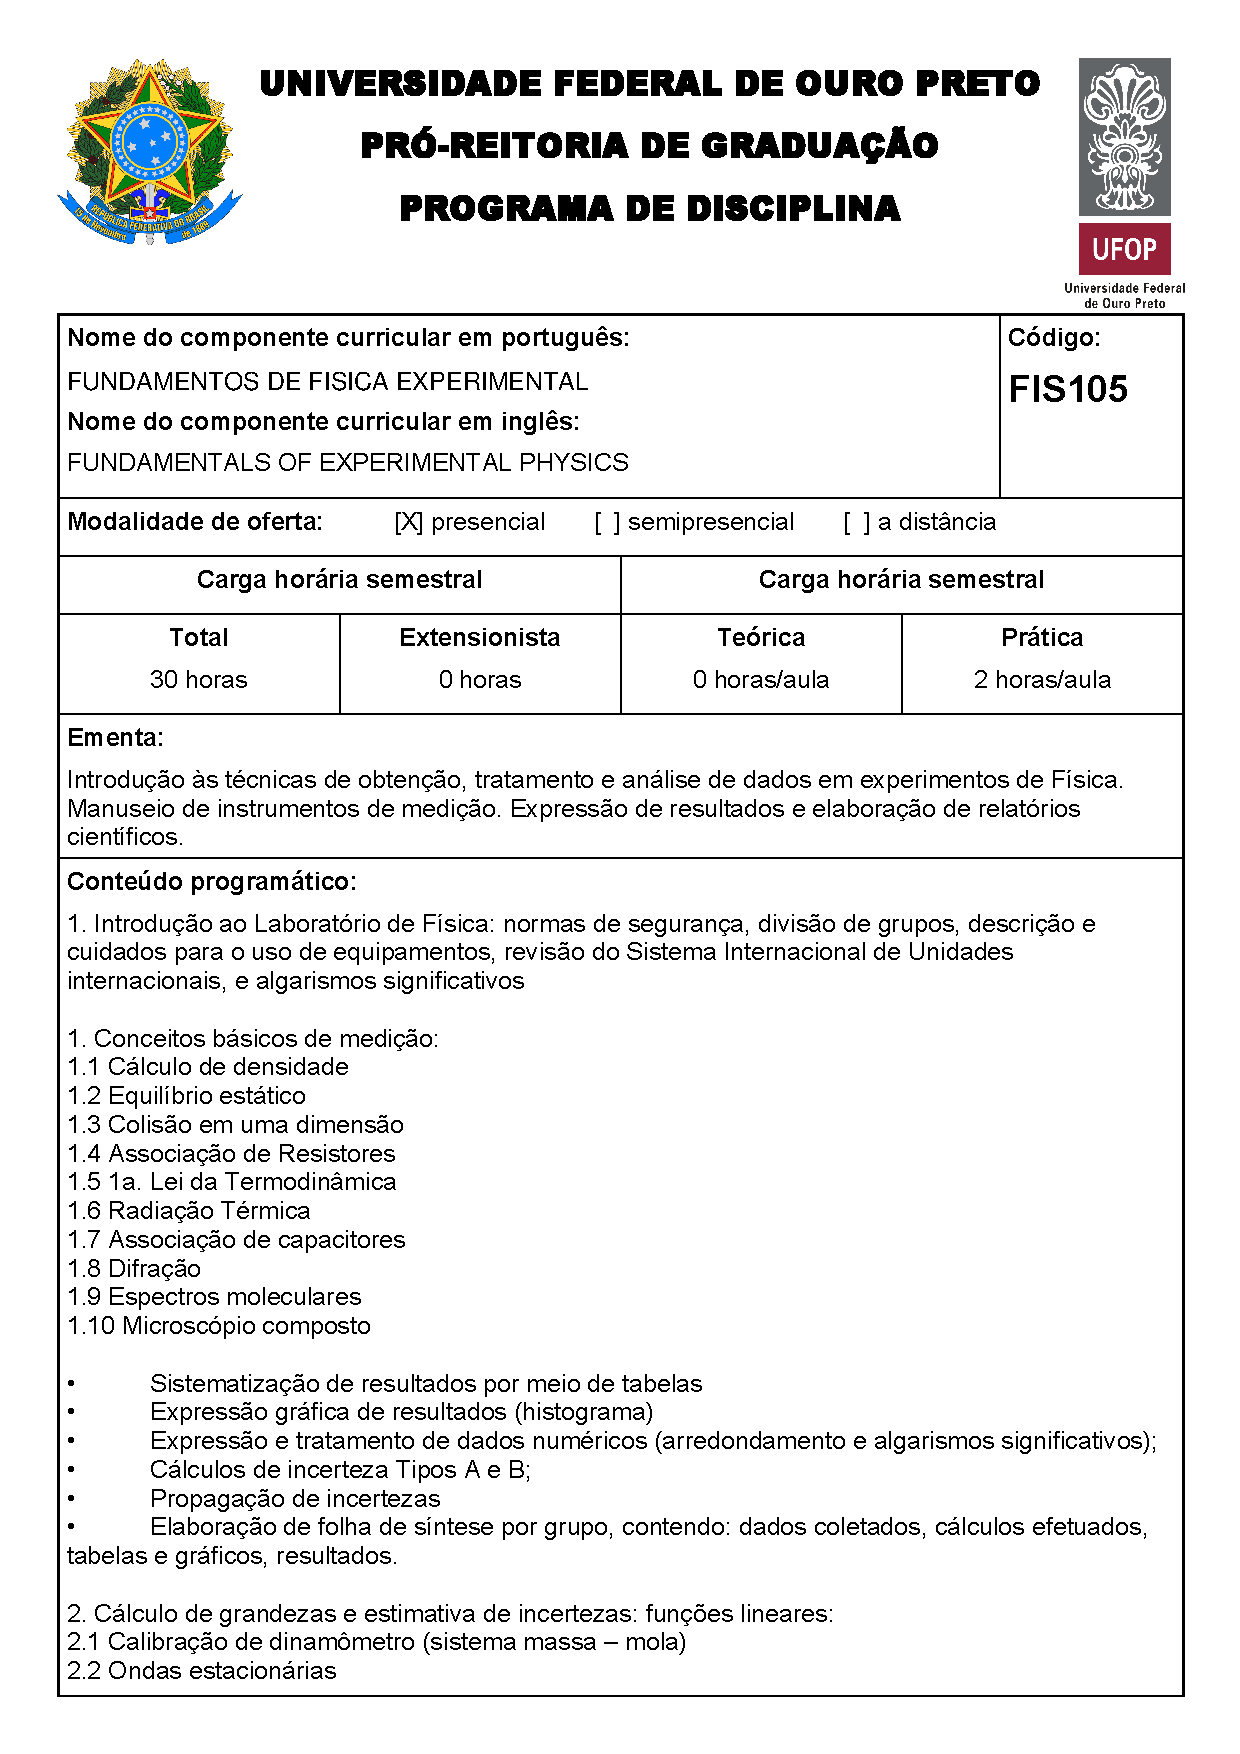
\includepdf[pages=-,nup=1x1, frame]{FIS105}
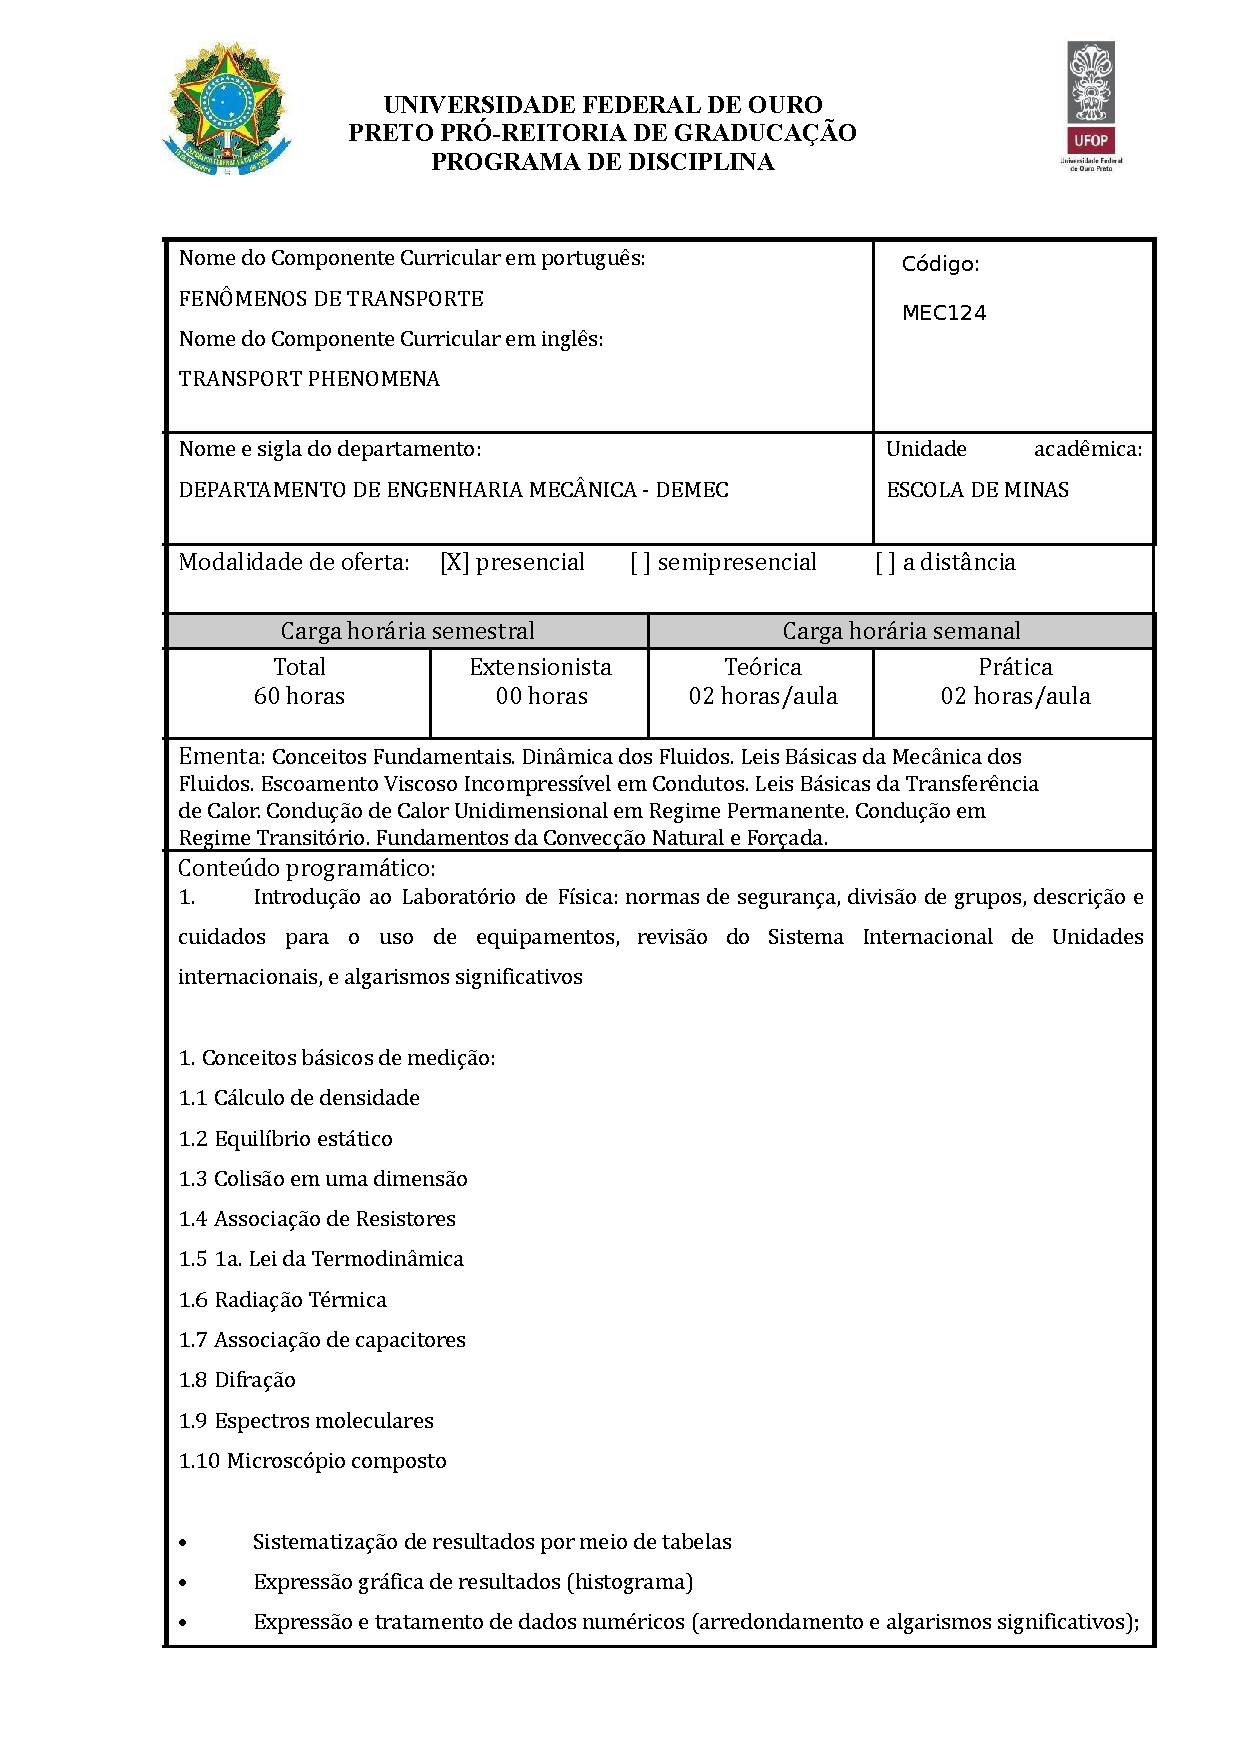
\includepdf[pages=-,nup=1x1, frame]{MEC124} %MECXX1
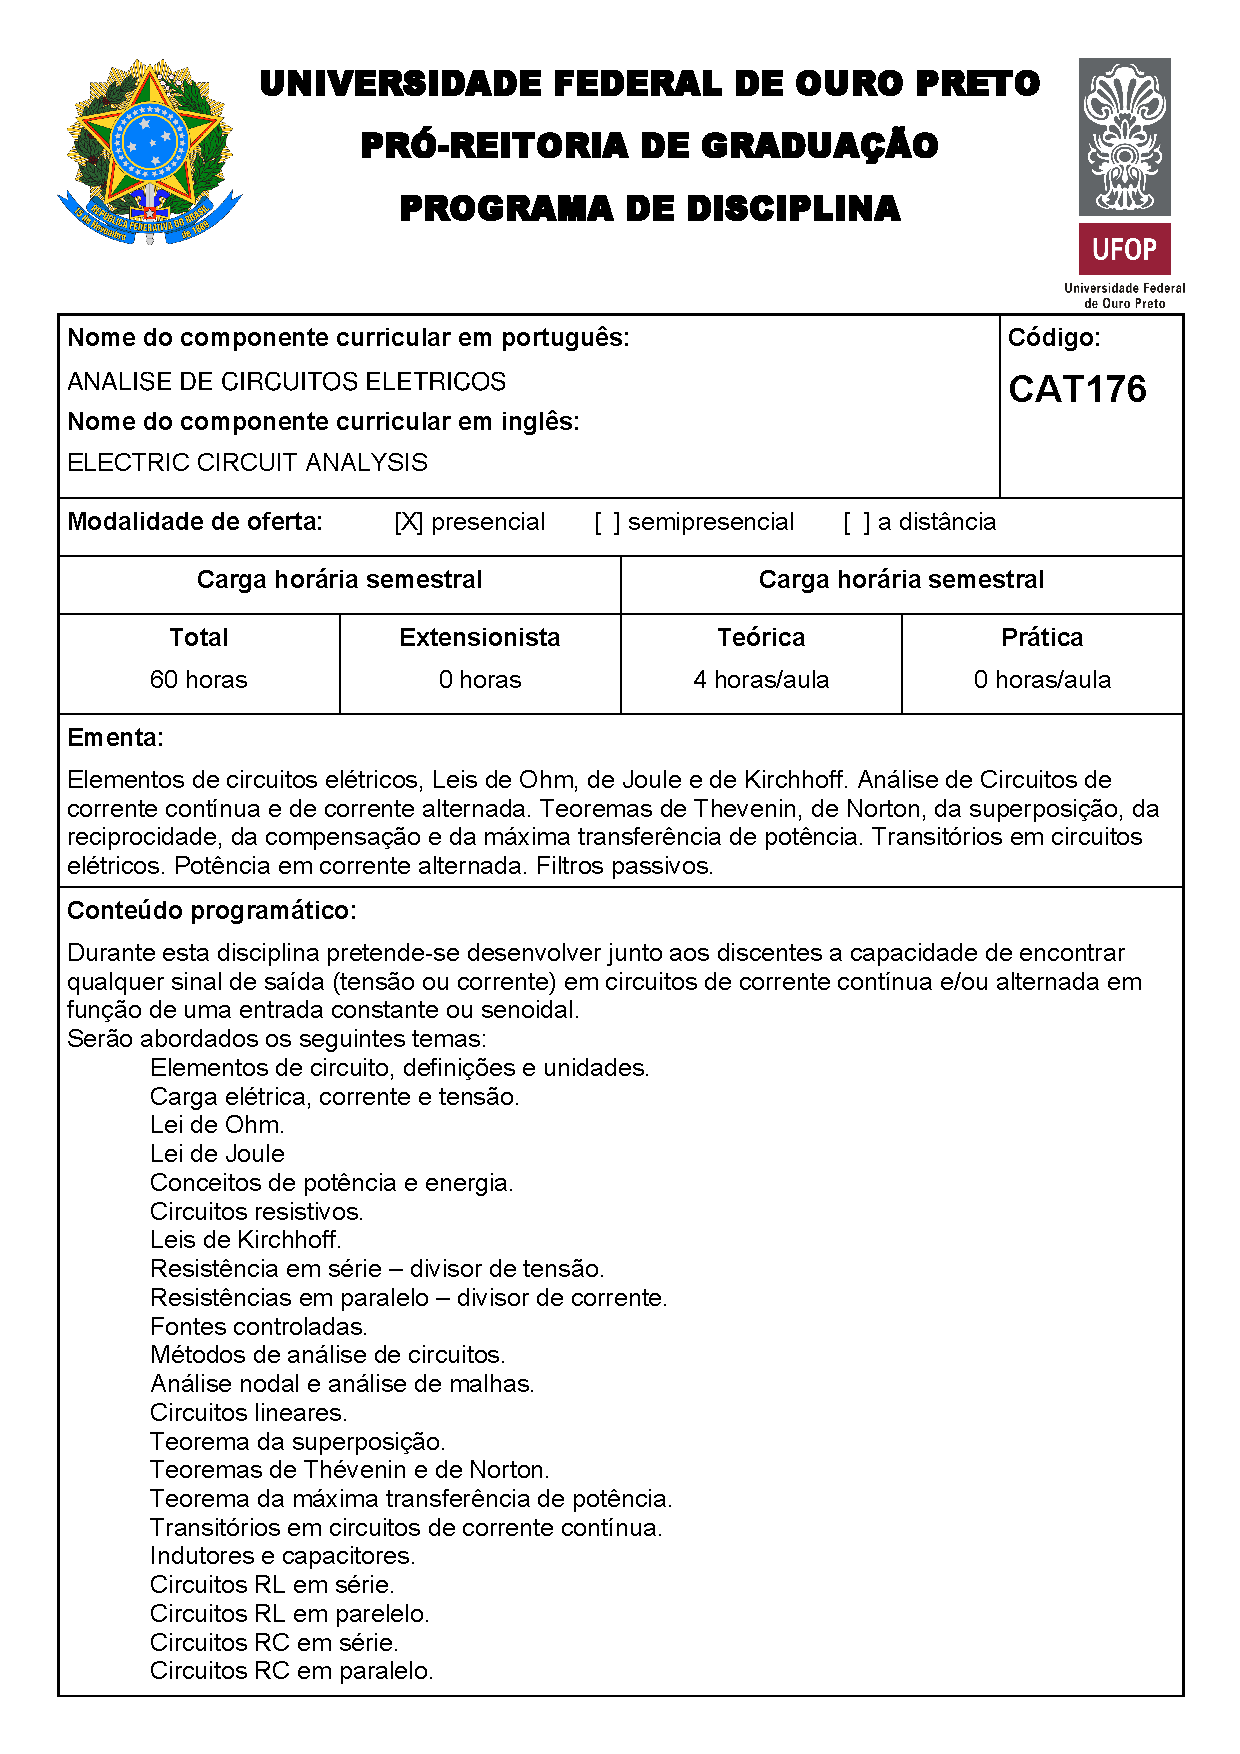
\includepdf[pages=-,nup=1x1, frame]{CAT176}
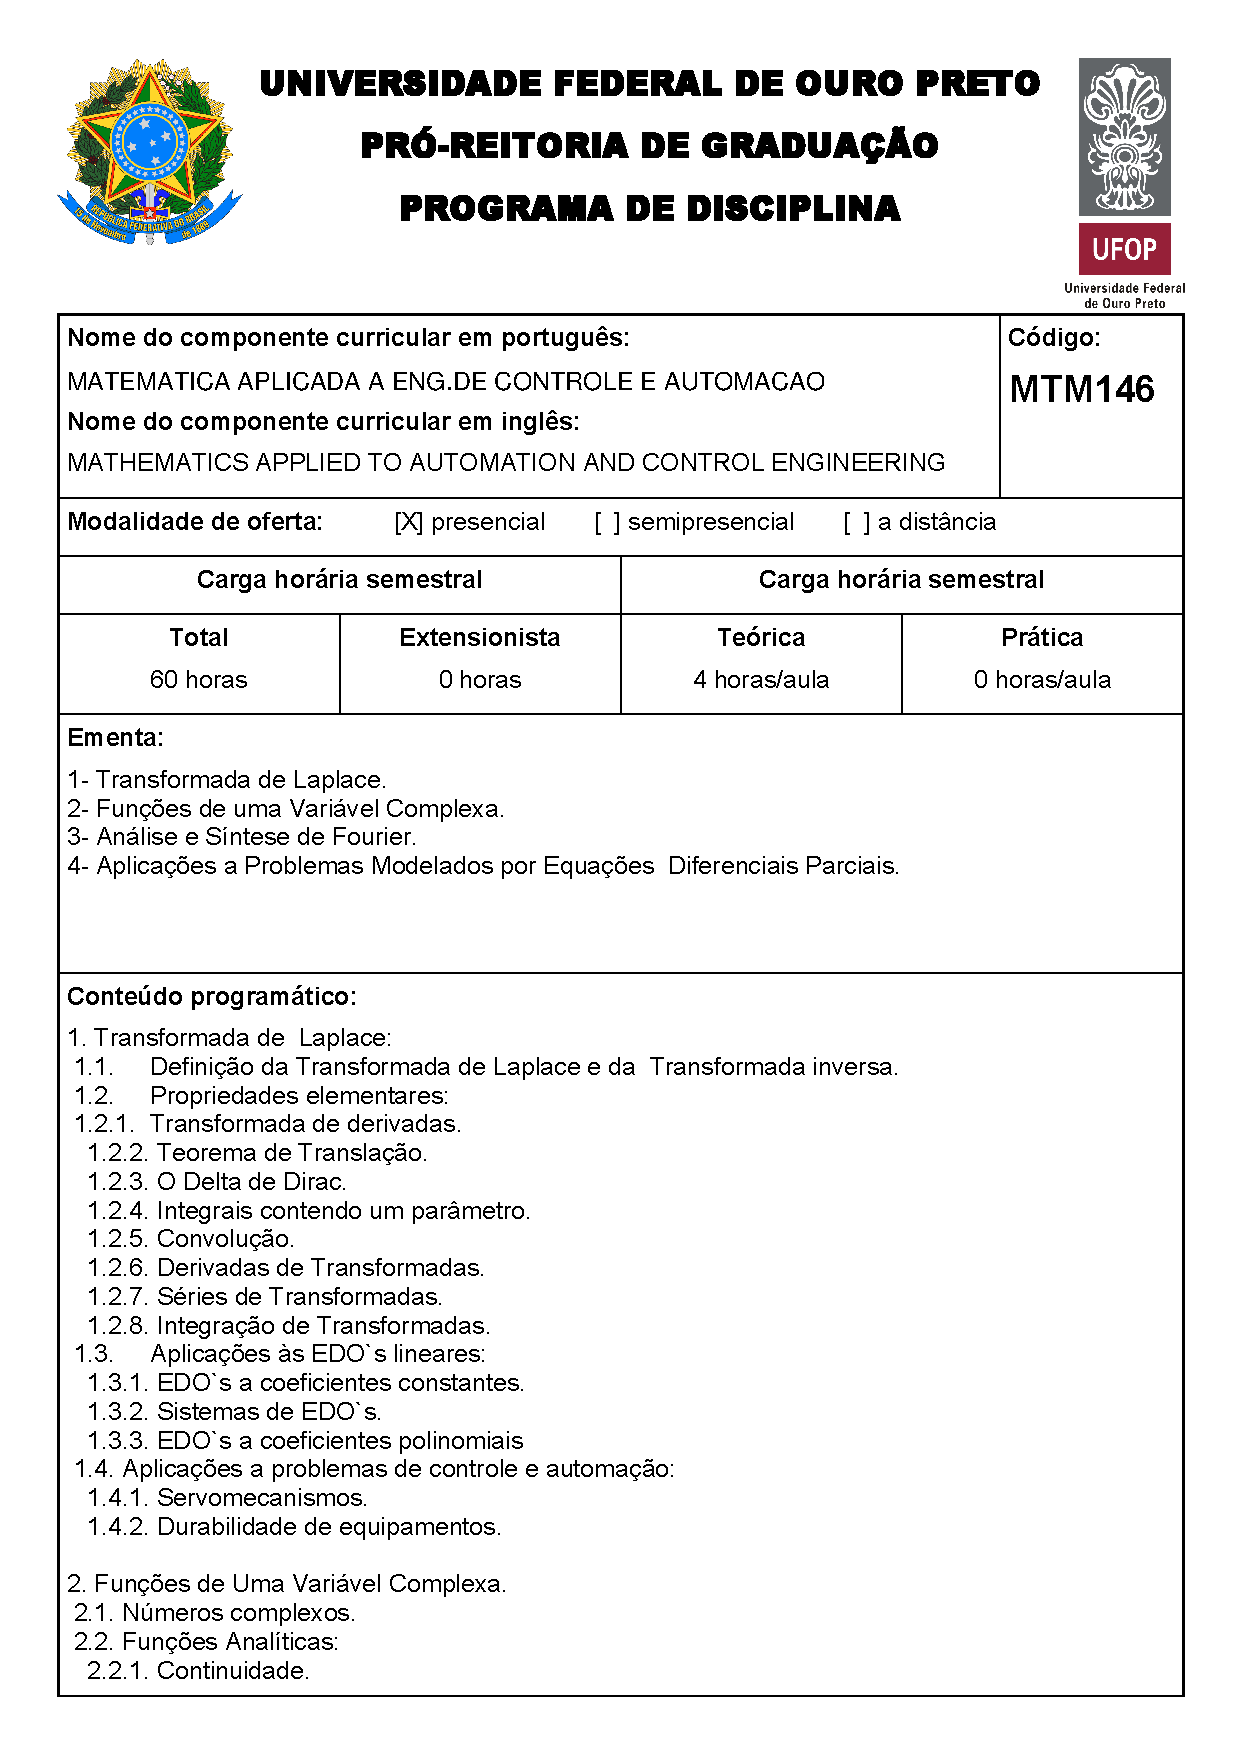
\includepdf[pages=-,nup=1x1, frame]{MTM146}
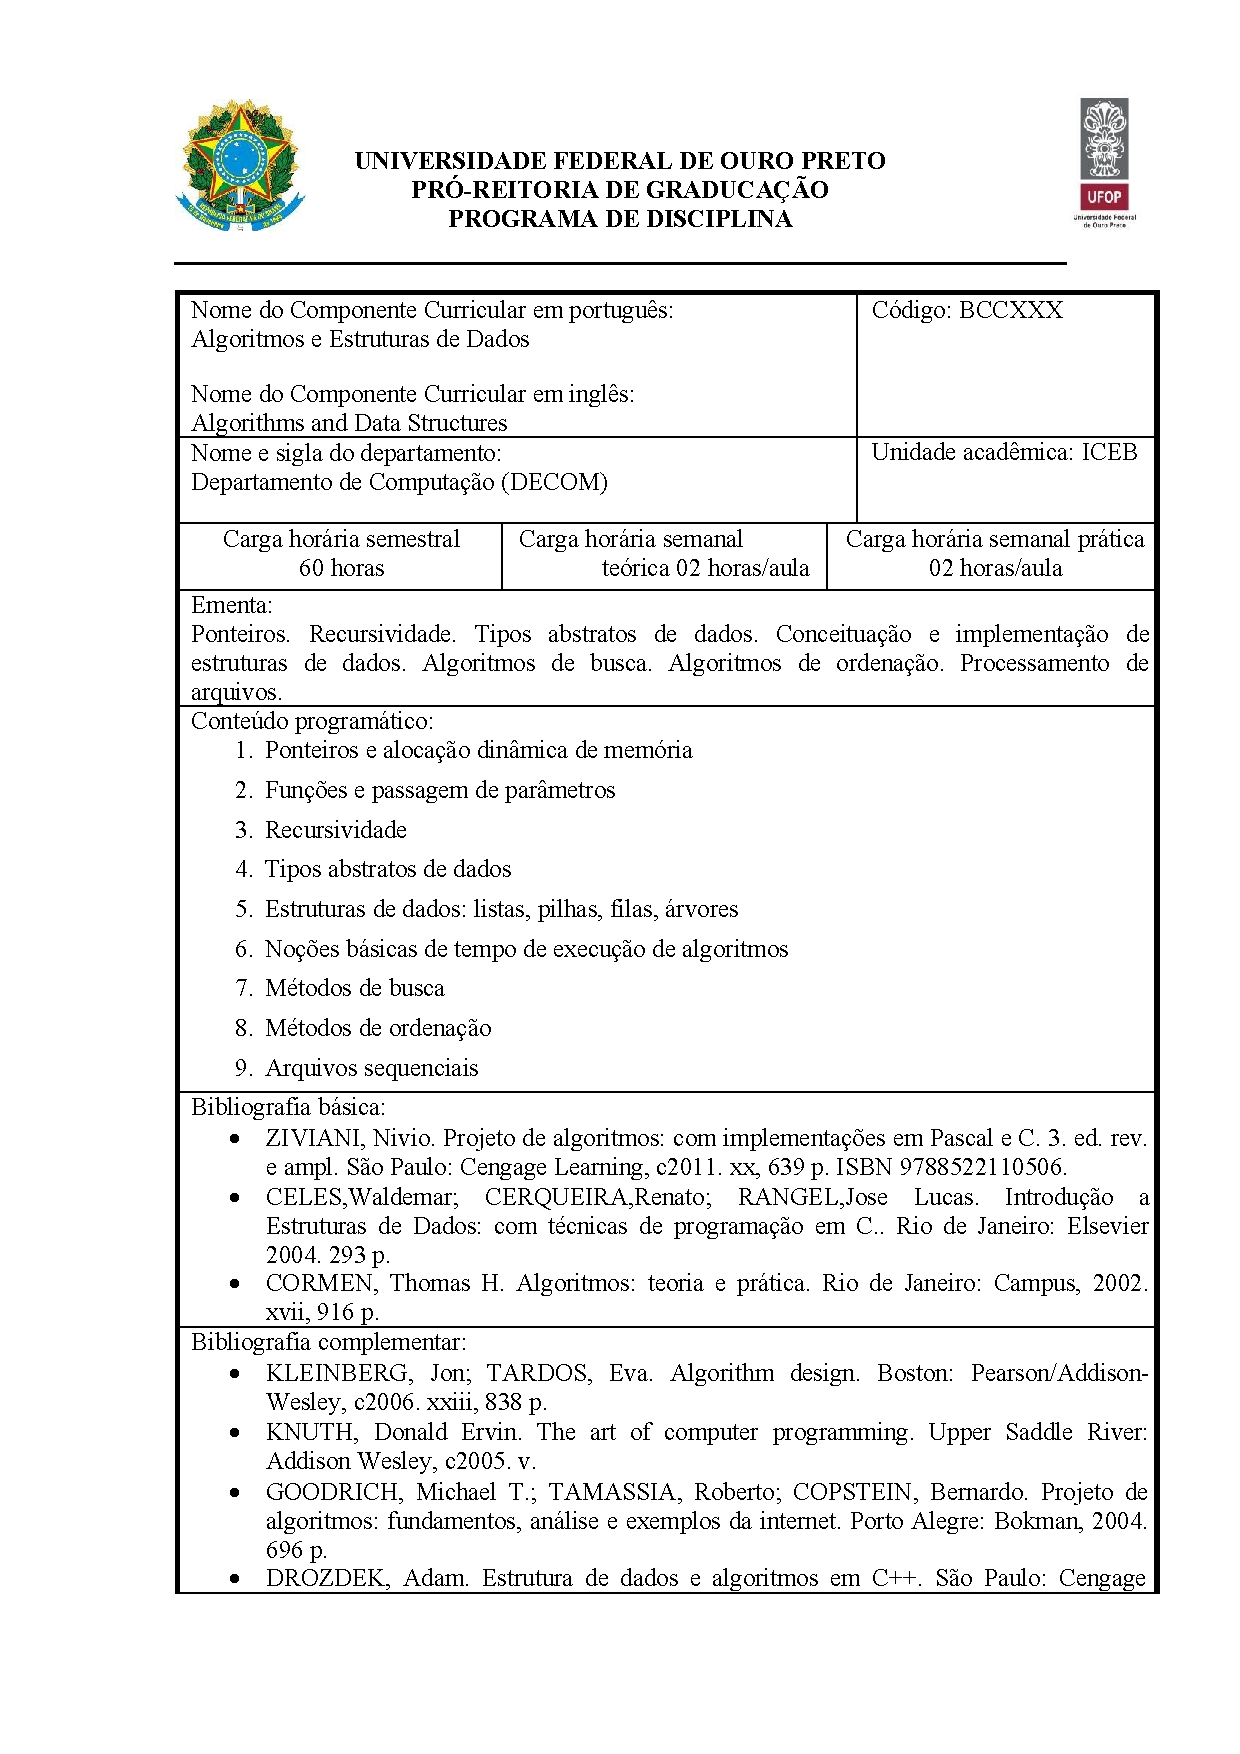
\includepdf[pages=-,nup=1x1, frame]{BCC704} % BCCXX3


% quinto semestre
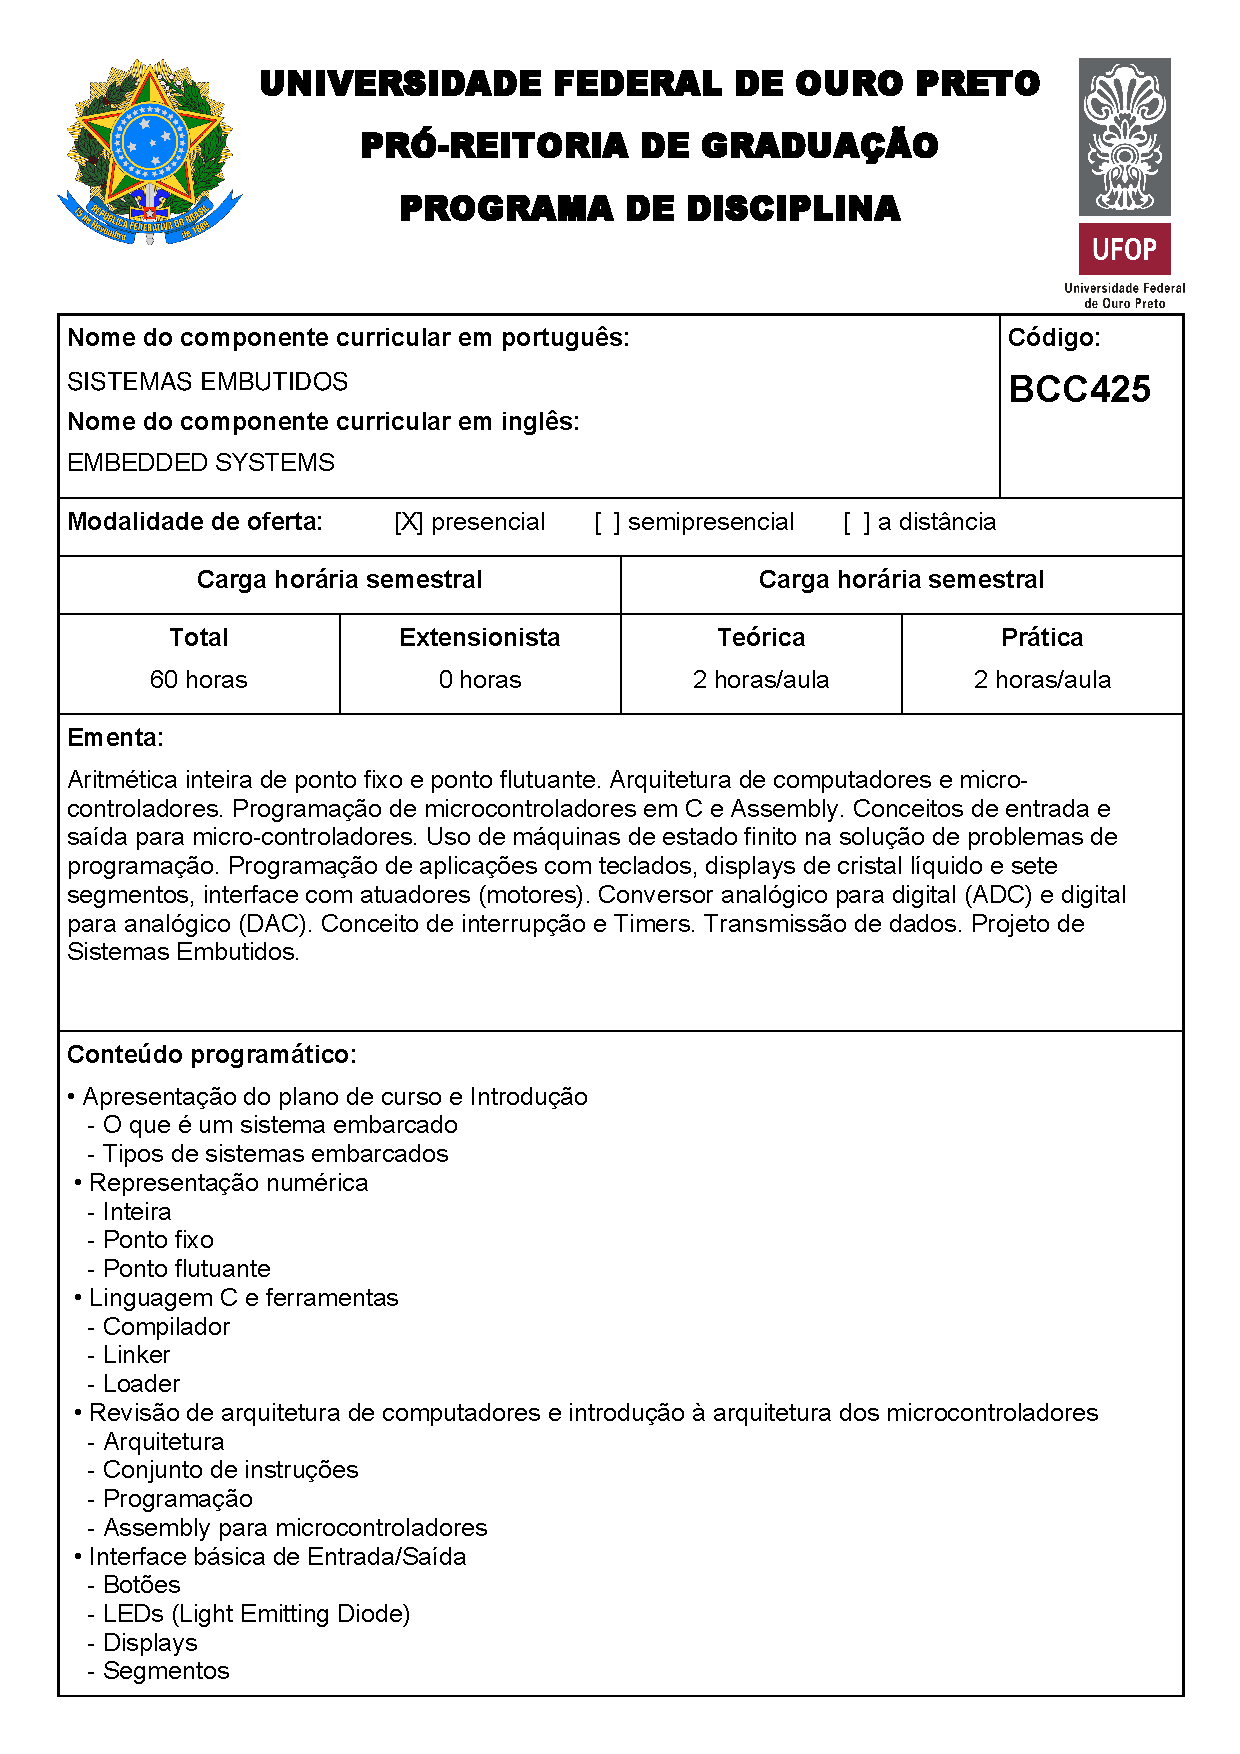
\includepdf[pages=-,nup=1x1, frame]{BCC425}
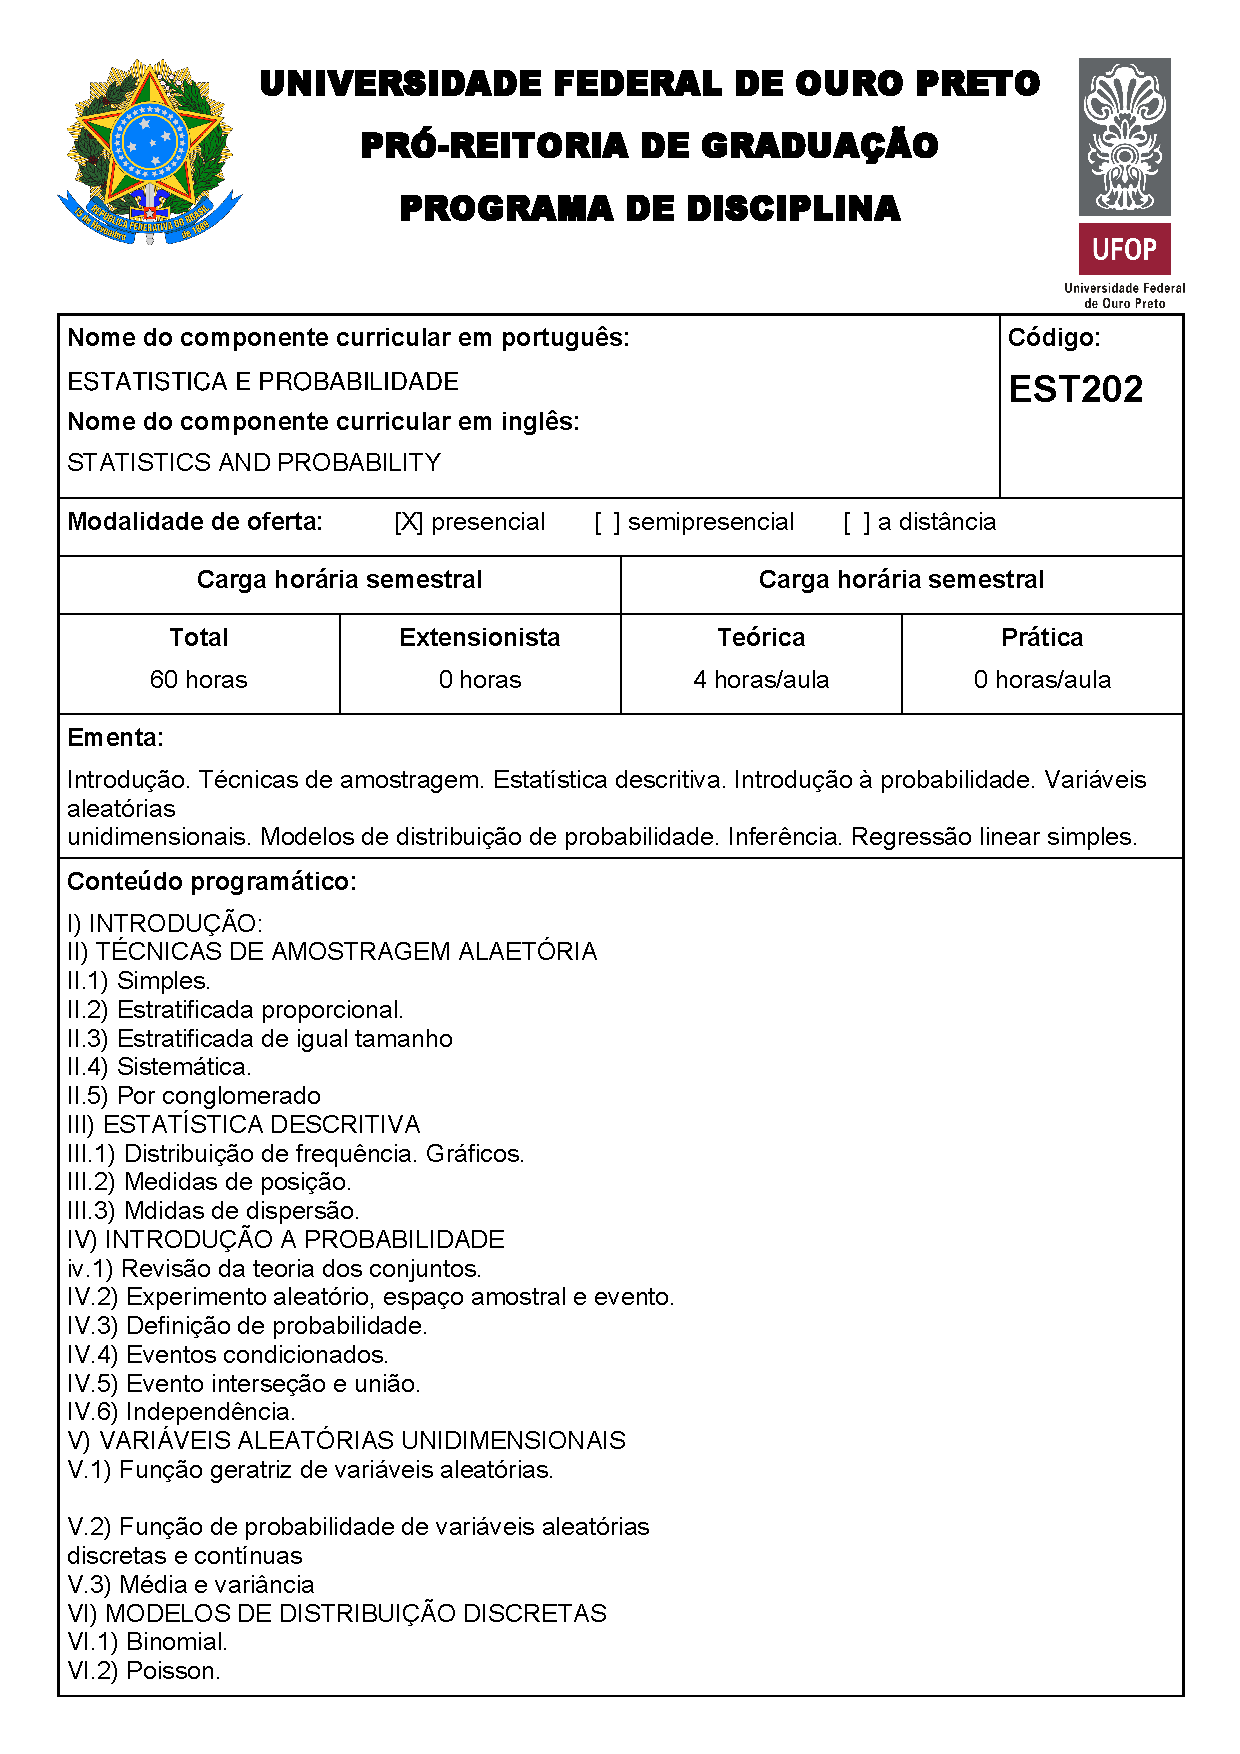
\includepdf[pages=-,nup=1x1, frame]{EST202}
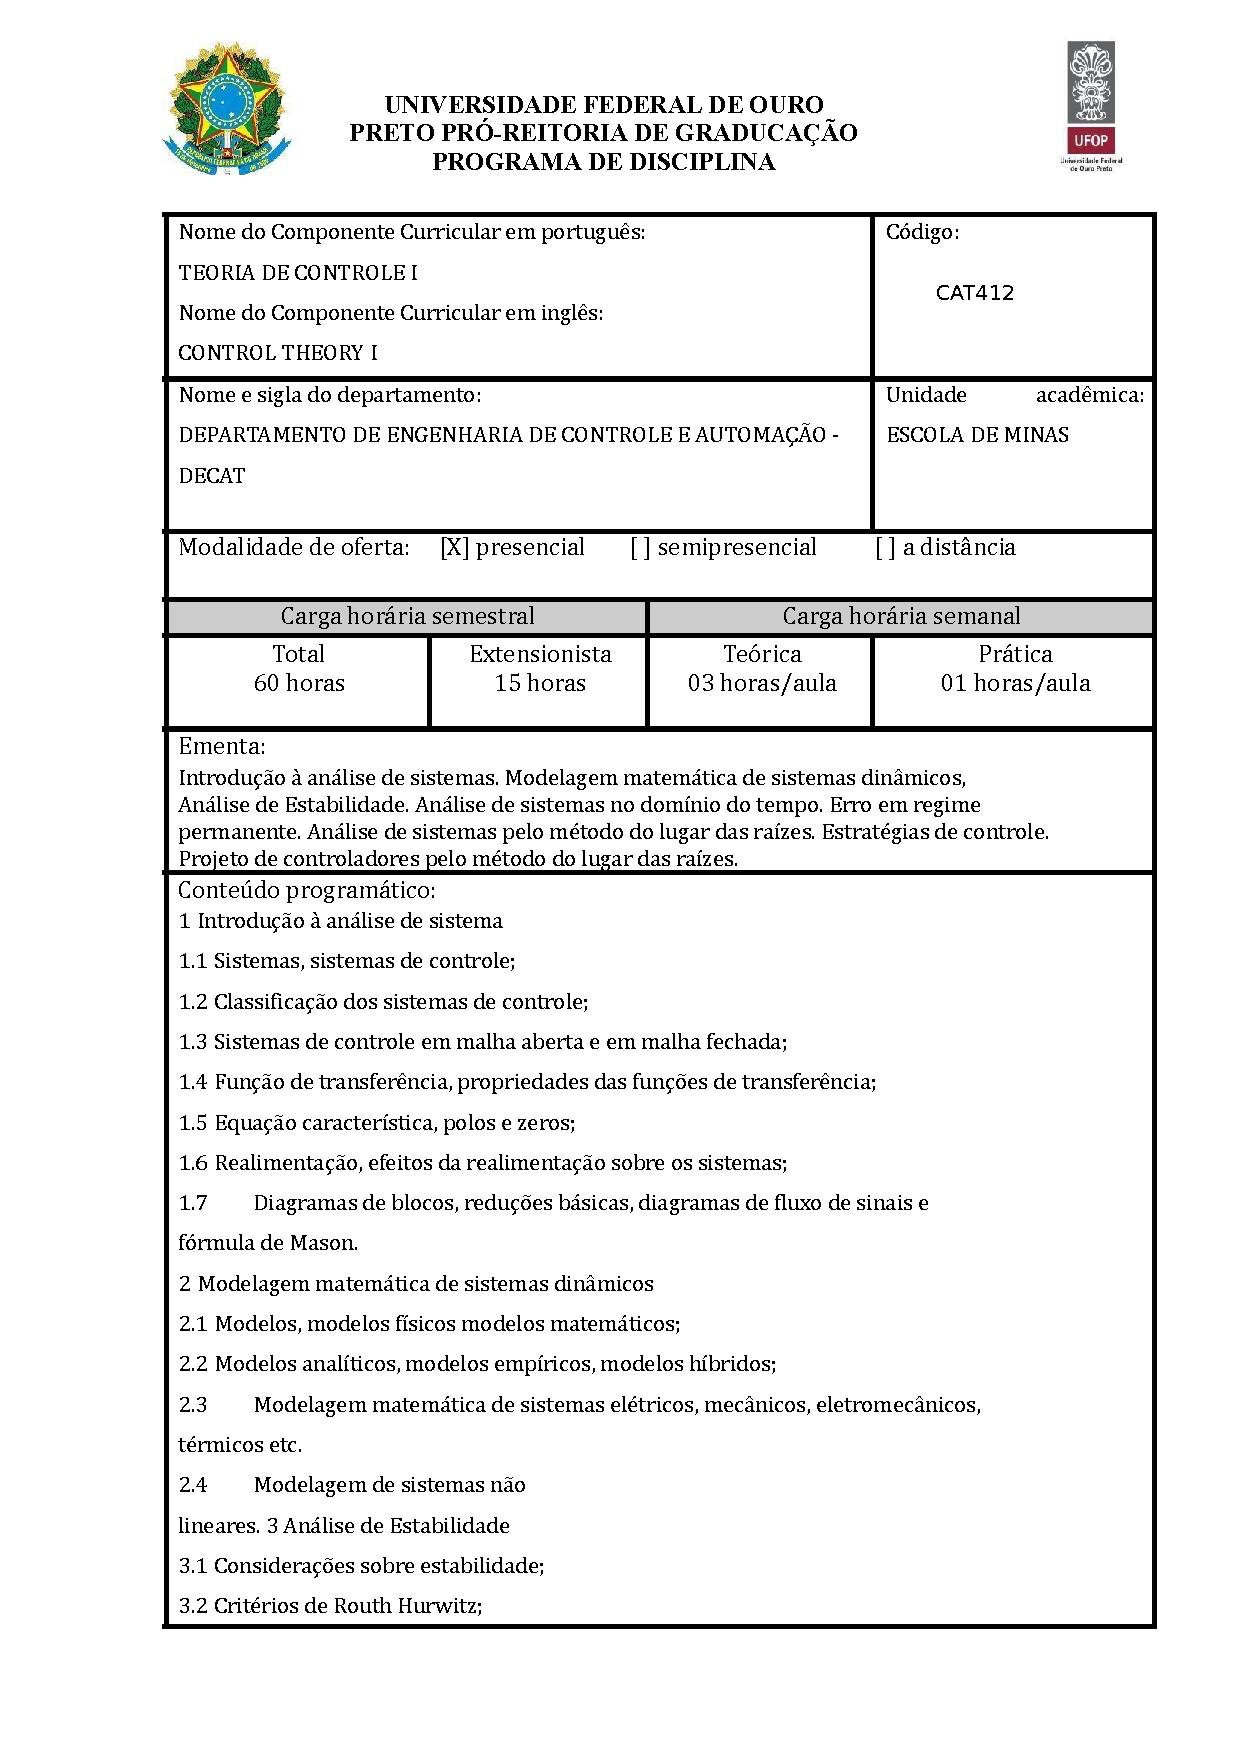
\includepdf[pages=-,nup=1x1, frame]{CAT412} % XXX003
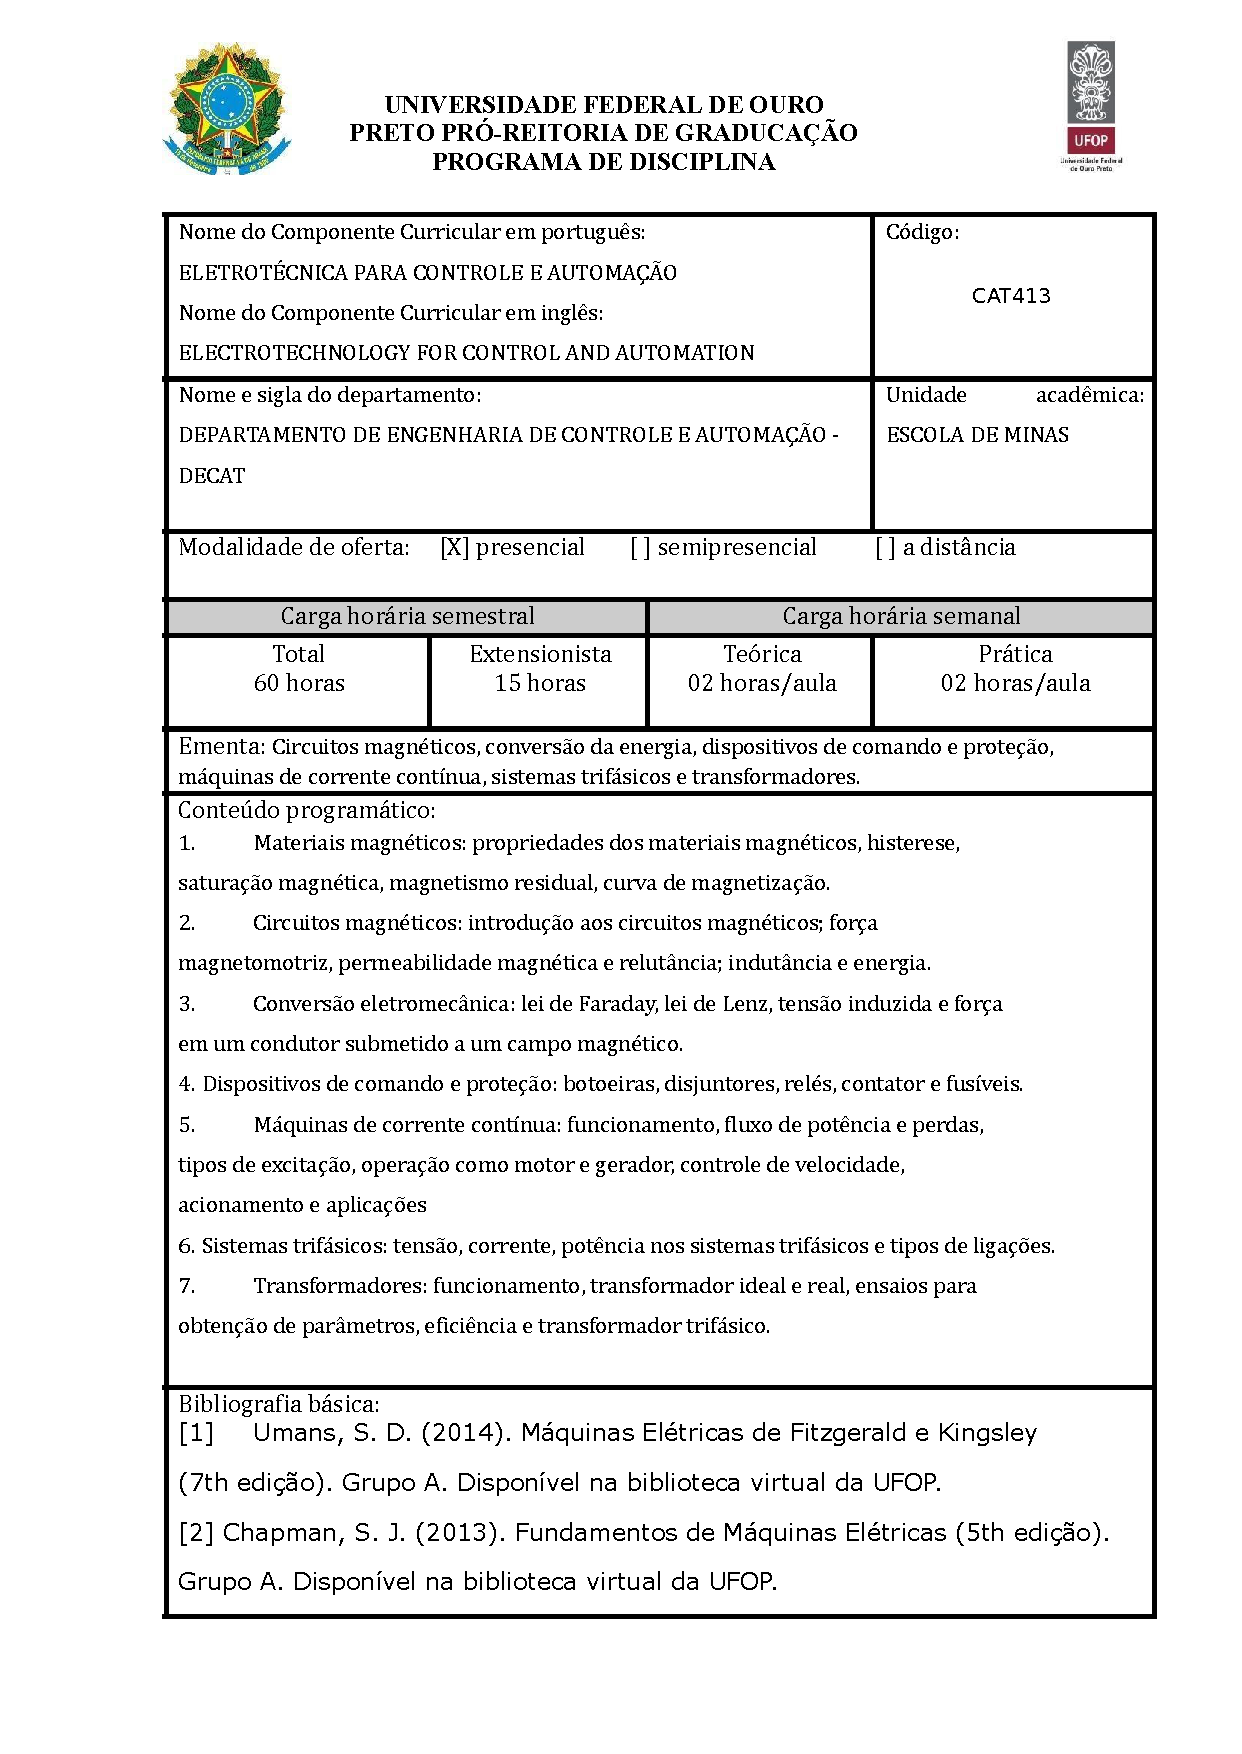
\includepdf[pages=-,nup=1x1, frame]{CAT413} % XXX004
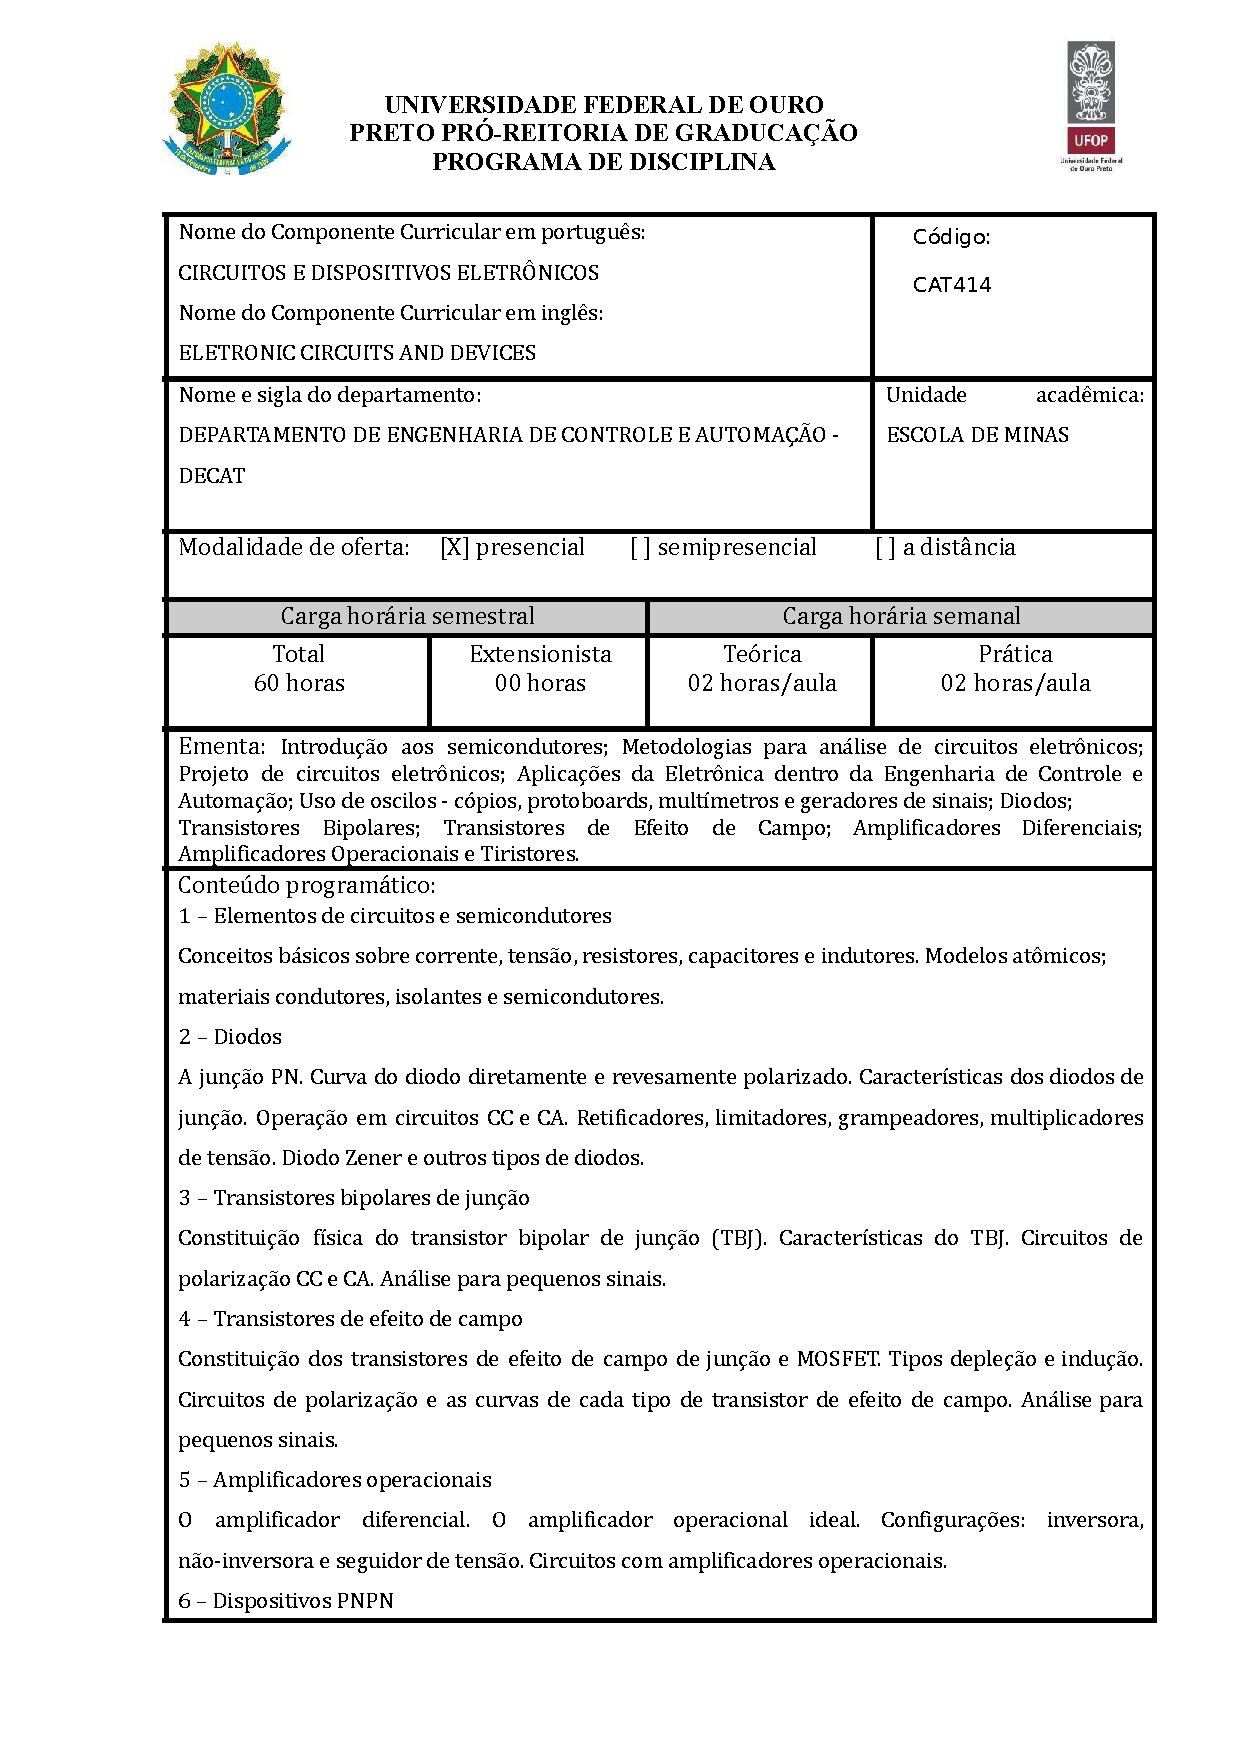
\includepdf[pages=-,nup=1x1, frame]{CAT414} % XXX029


%sexto semestre
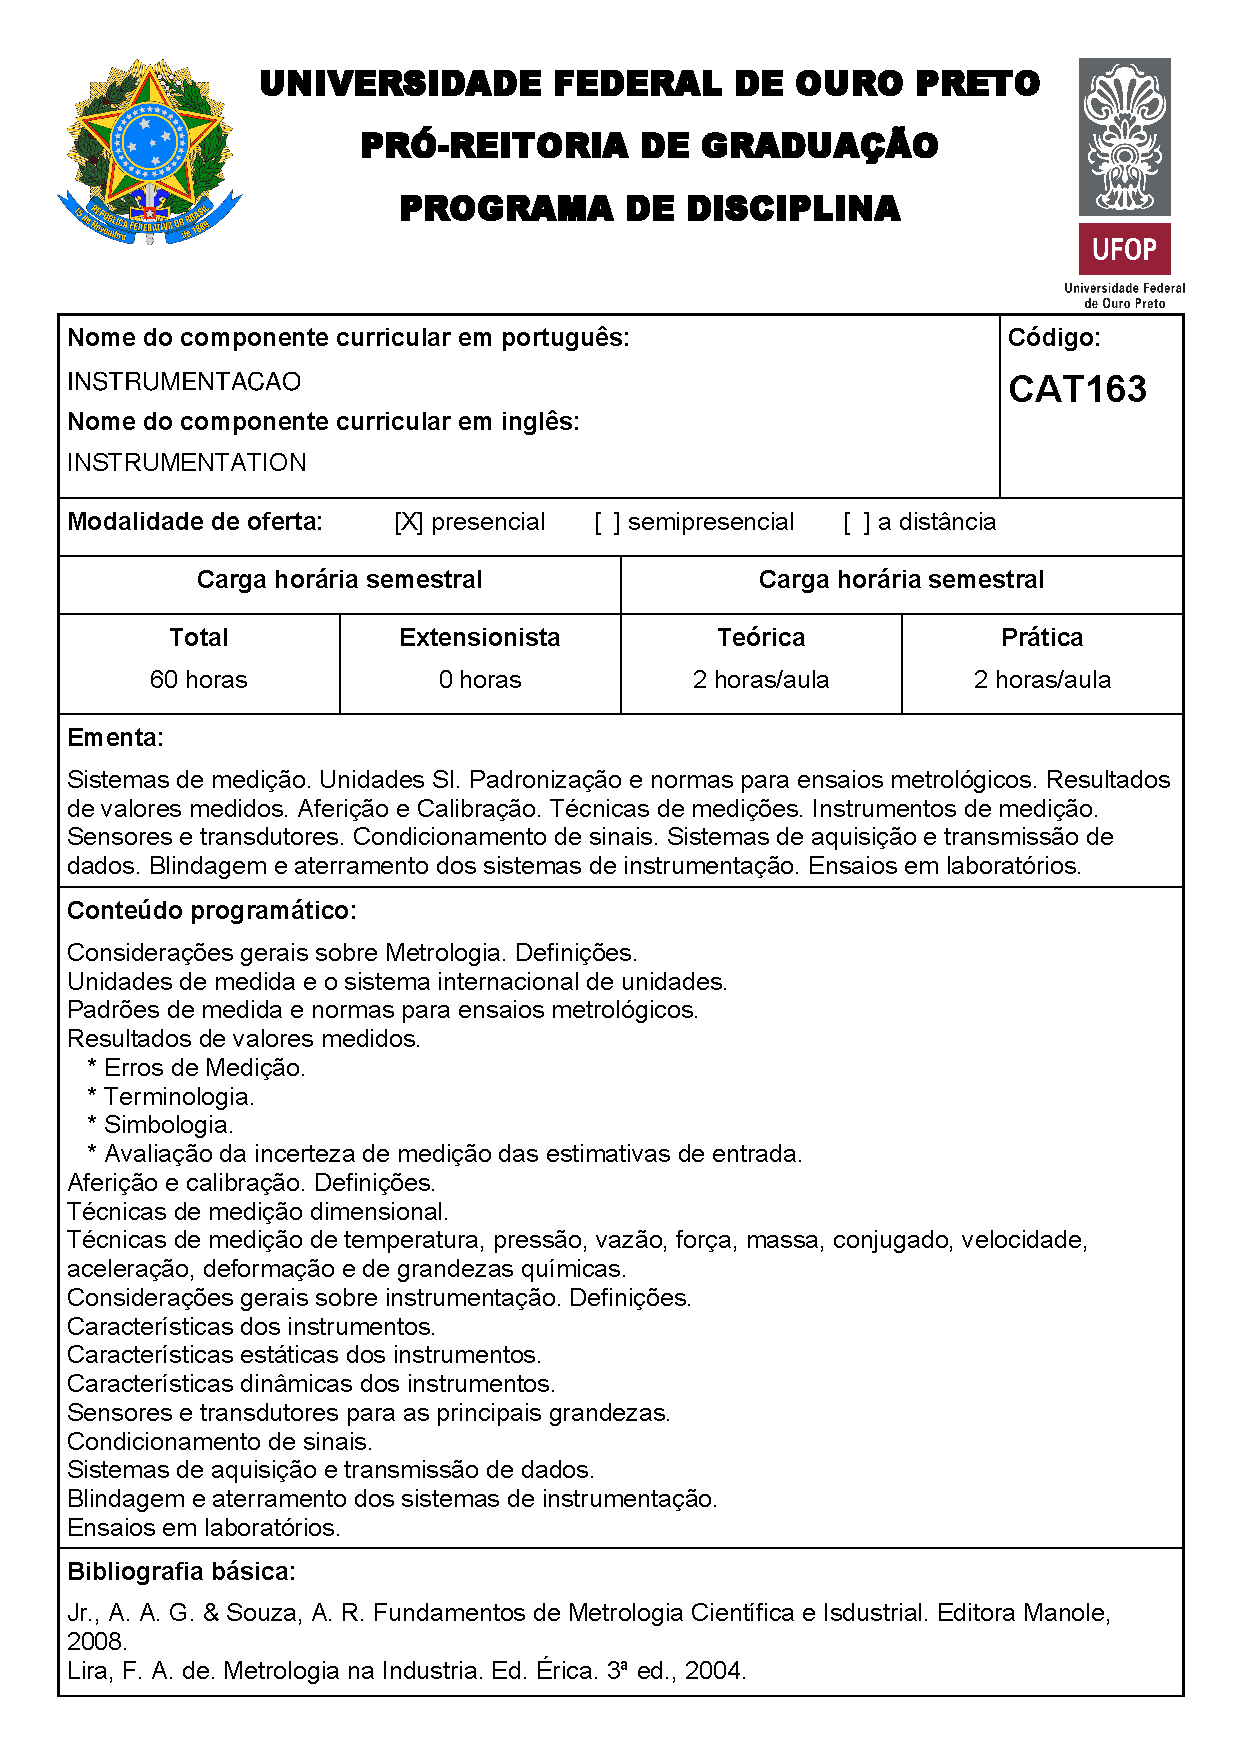
\includepdf[pages=-,nup=1x1, frame]{CAT163}
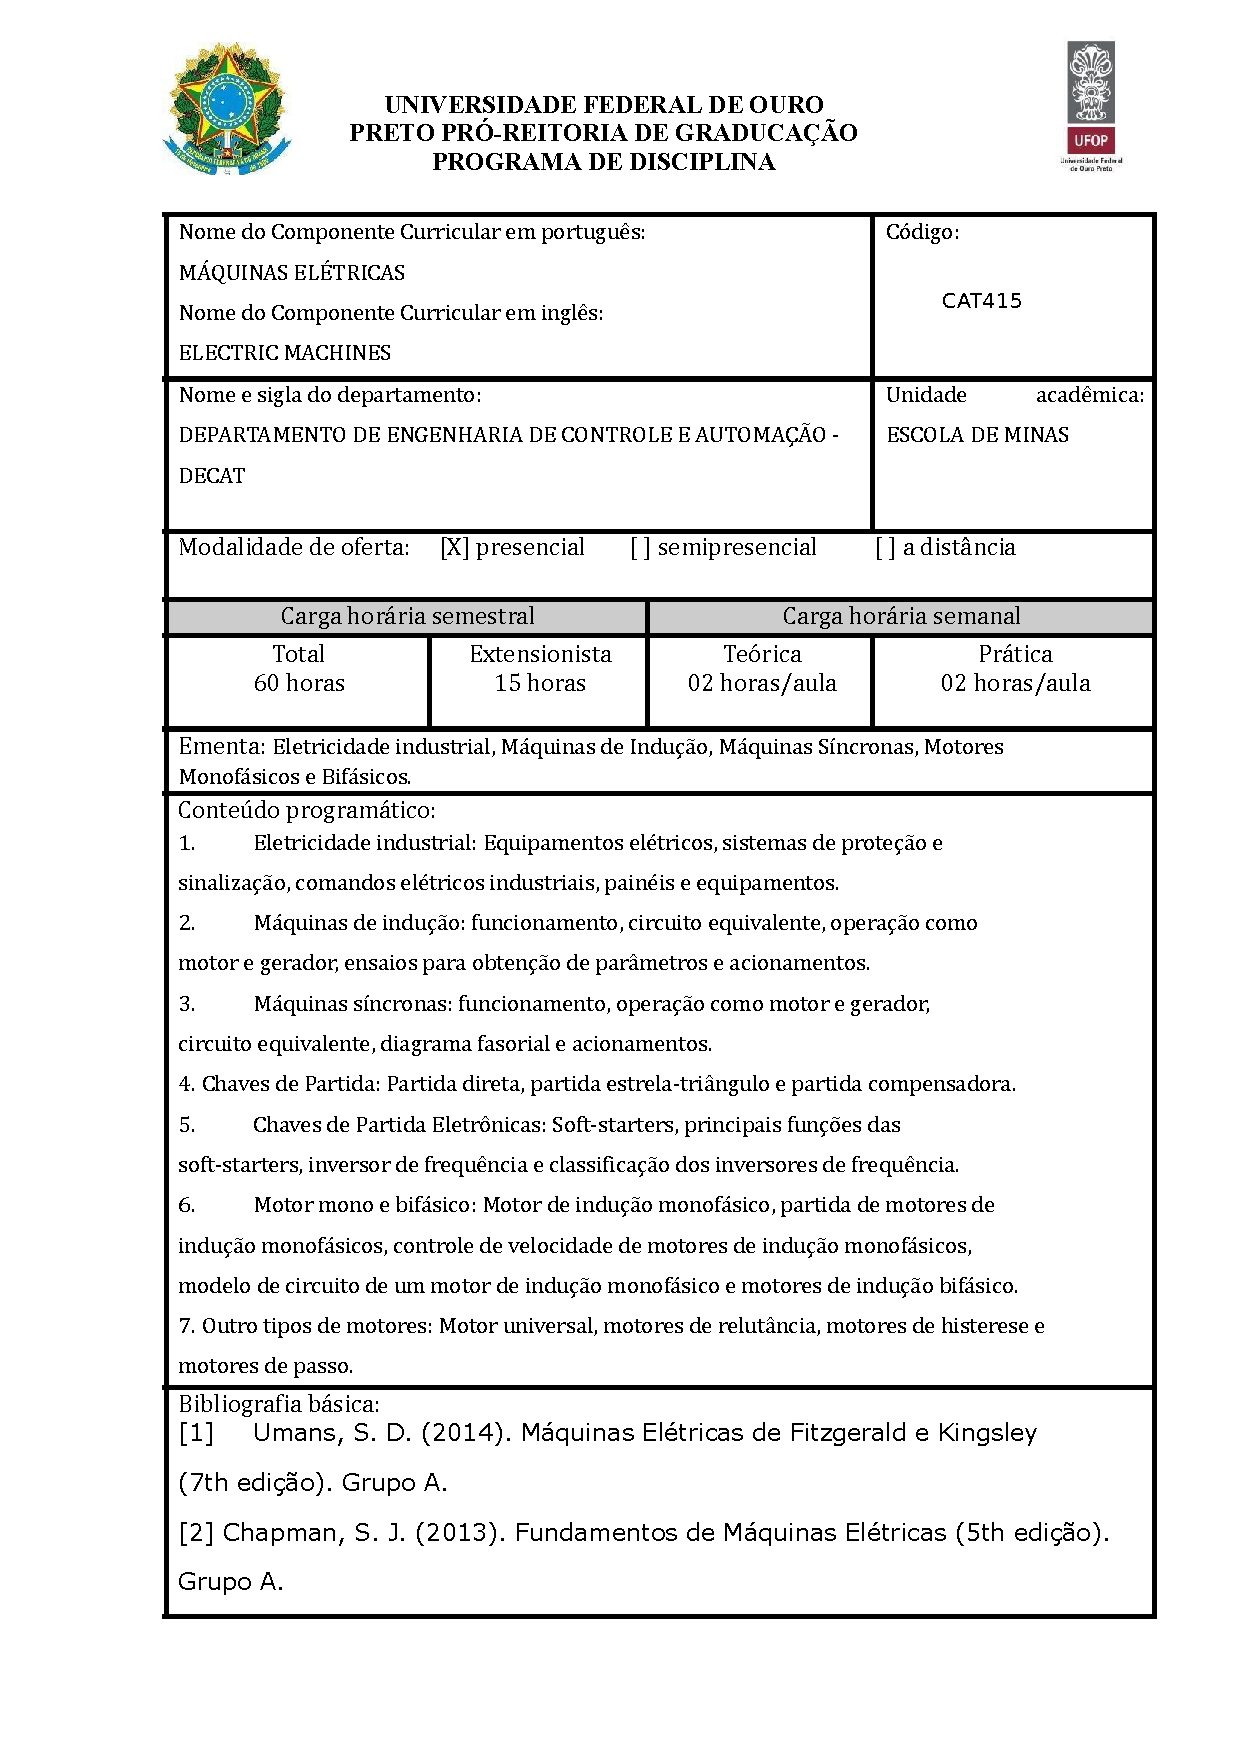
\includepdf[pages=-,nup=1x1, frame]{CAT415} % XXX005
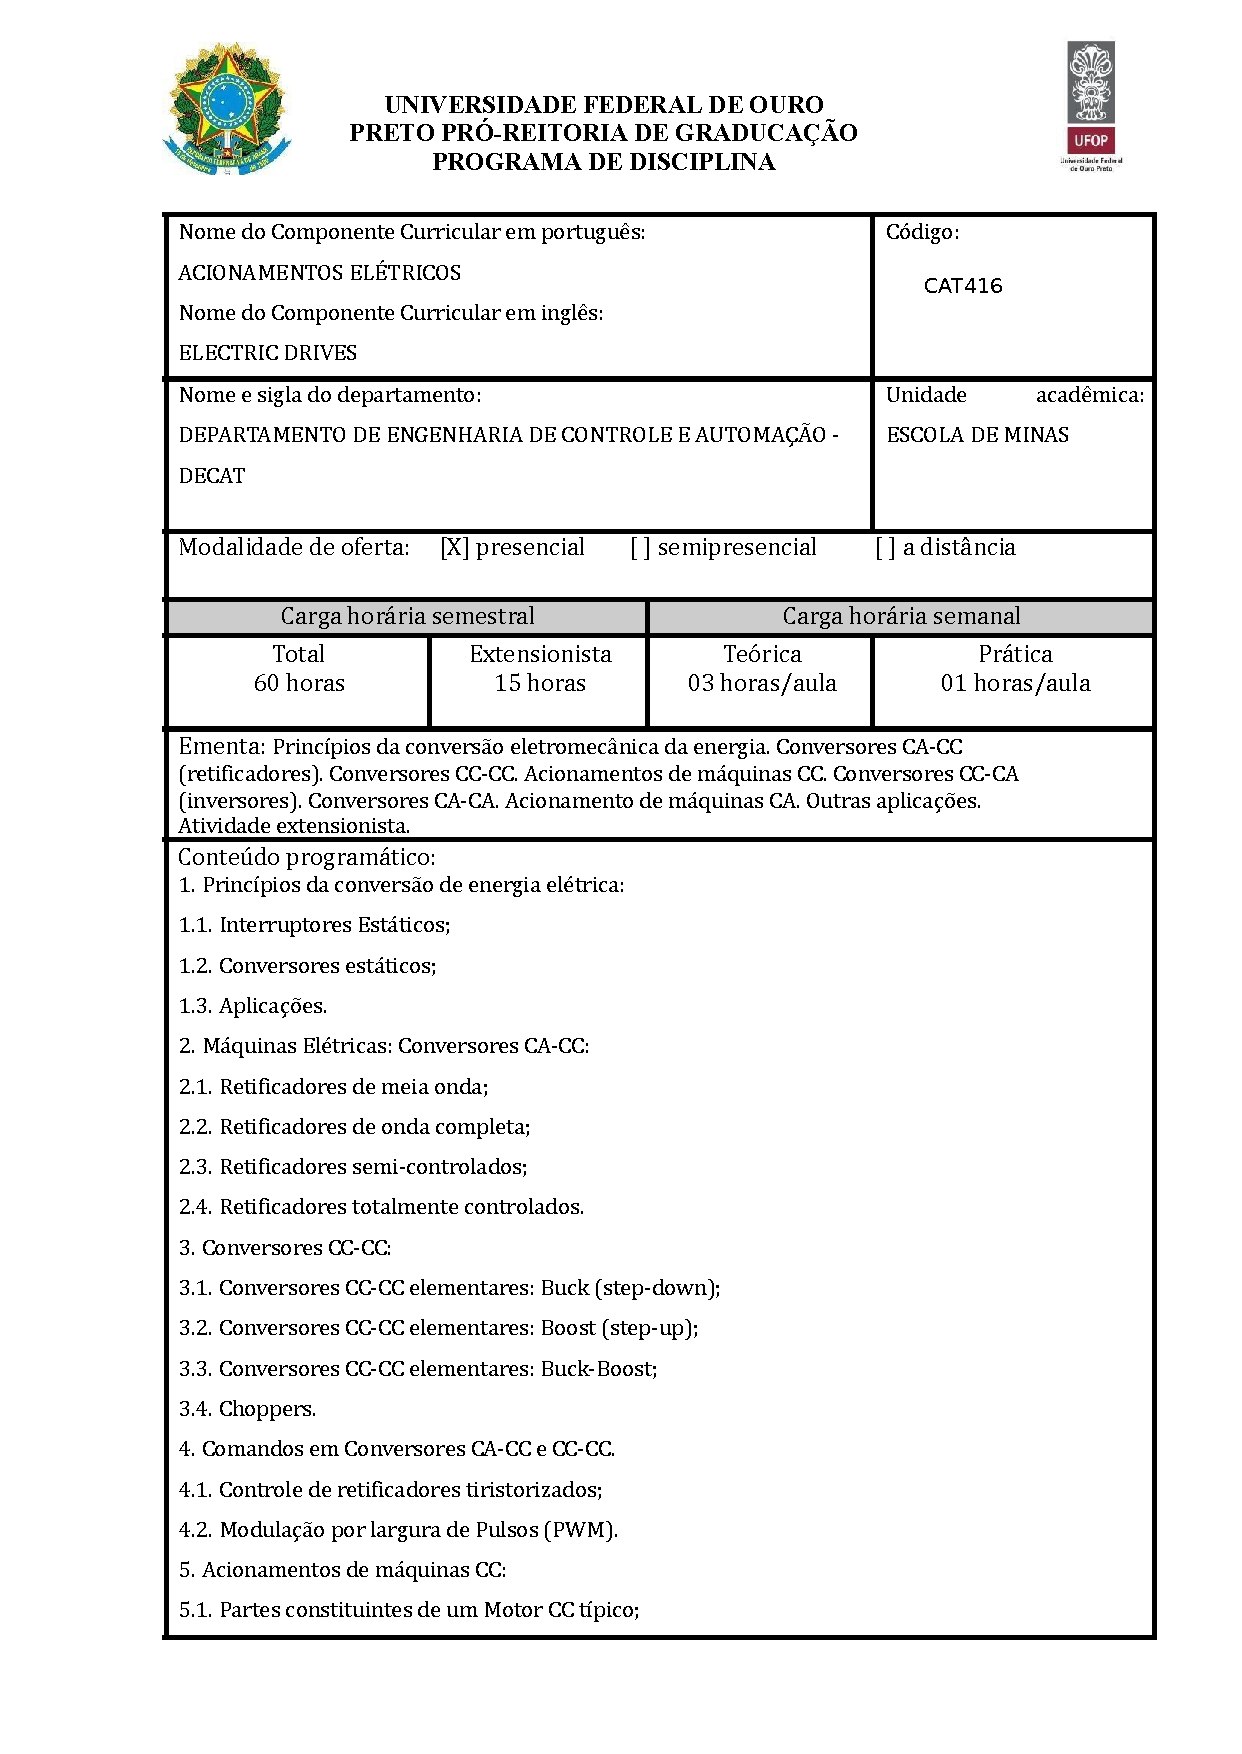
\includepdf[pages=-,nup=1x1, frame]{CAT416} % XXX006
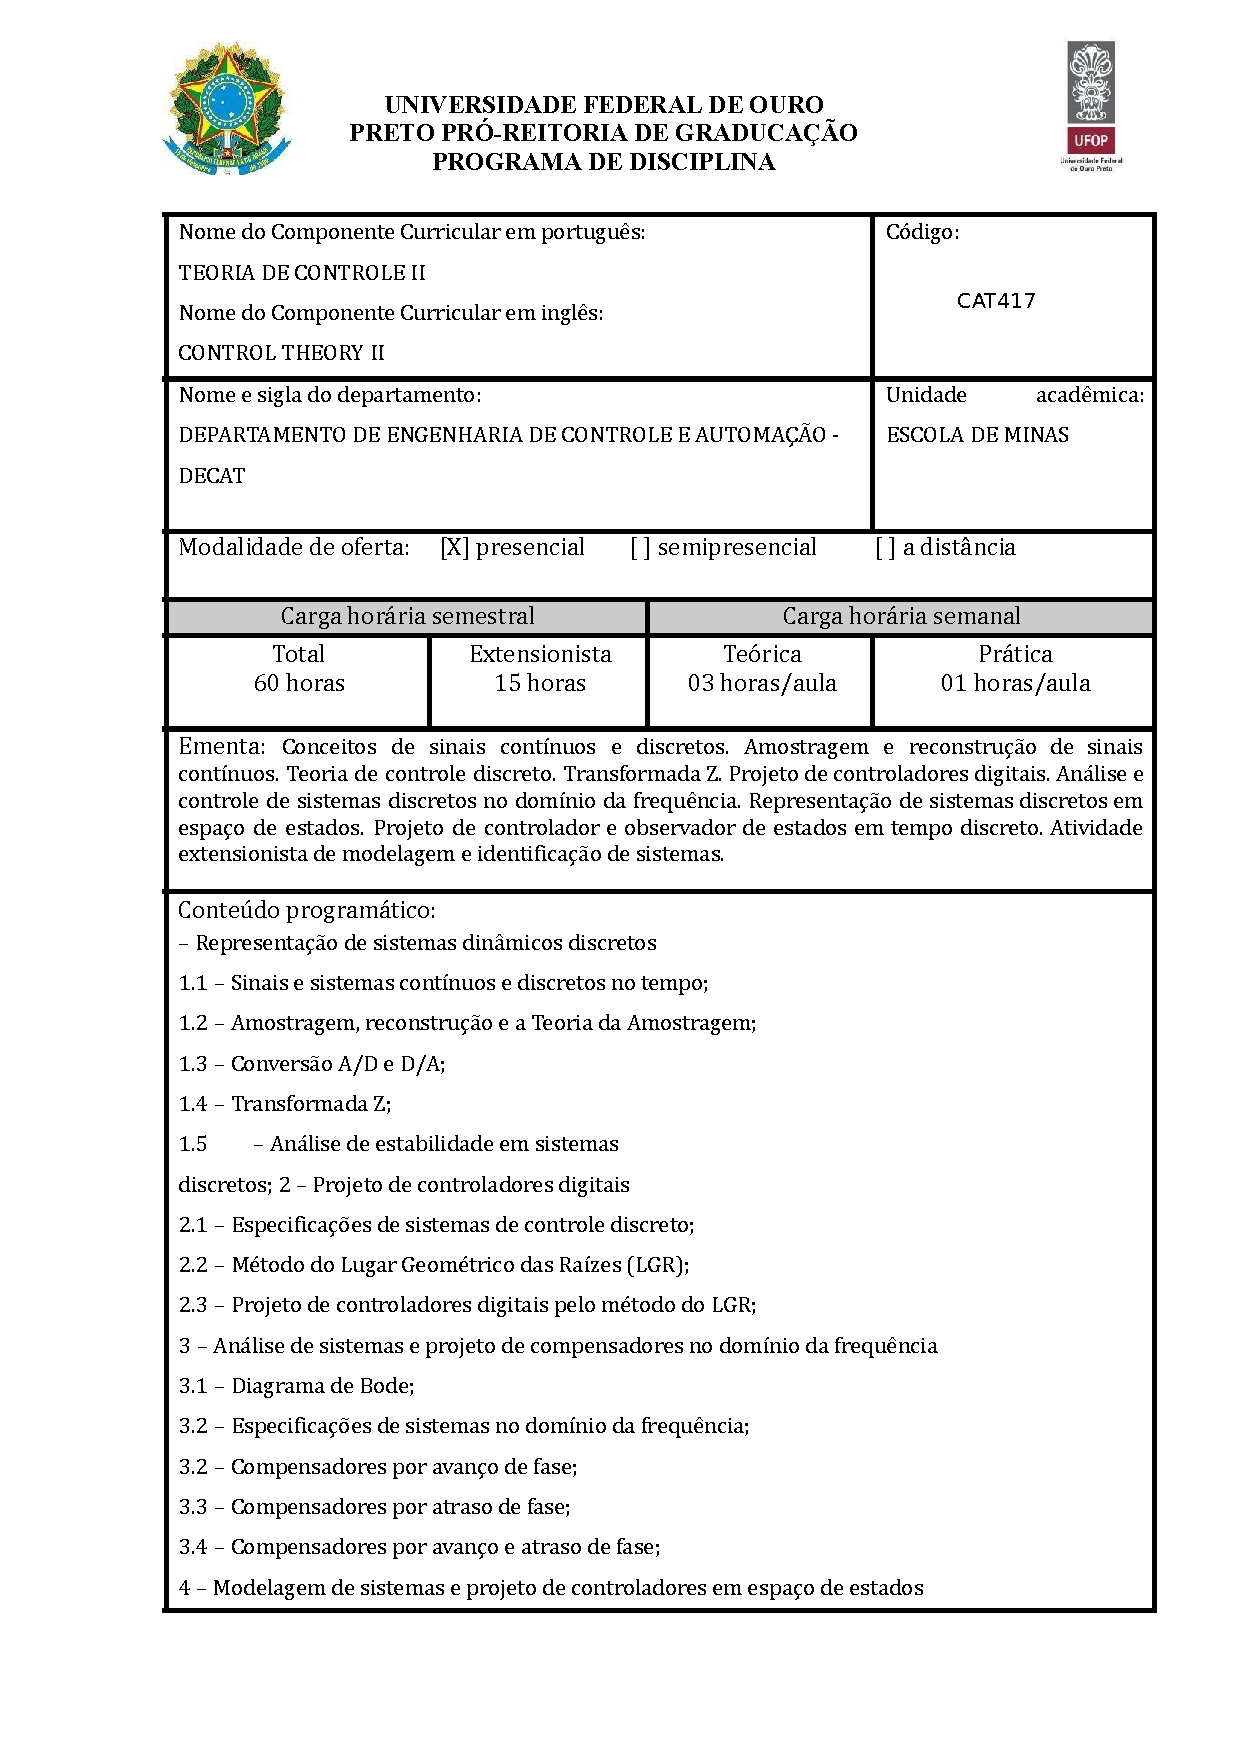
\includepdf[pages=-,nup=1x1, frame]{CAT417} % XXX007
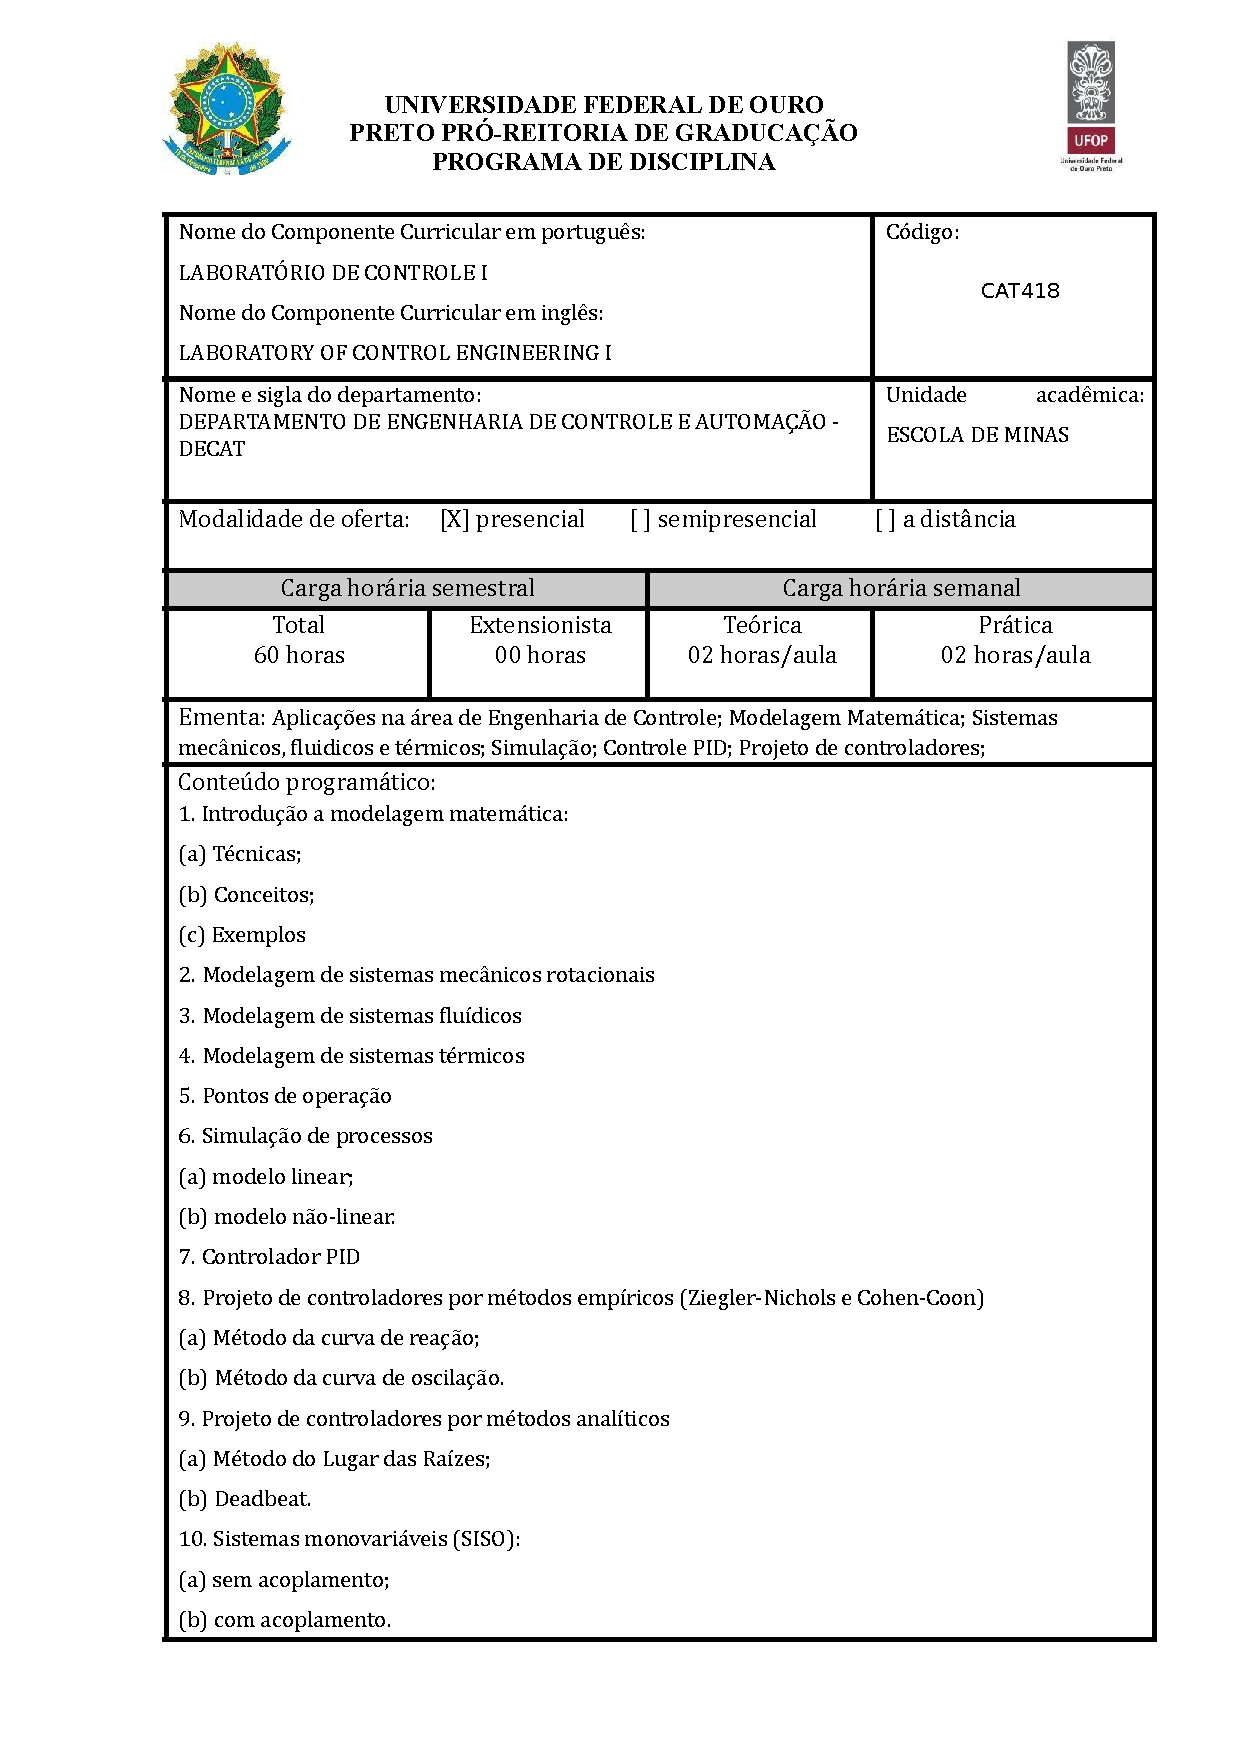
\includepdf[pages=-,nup=1x1, frame]{CAT418} % XXX008


%setimo semestre
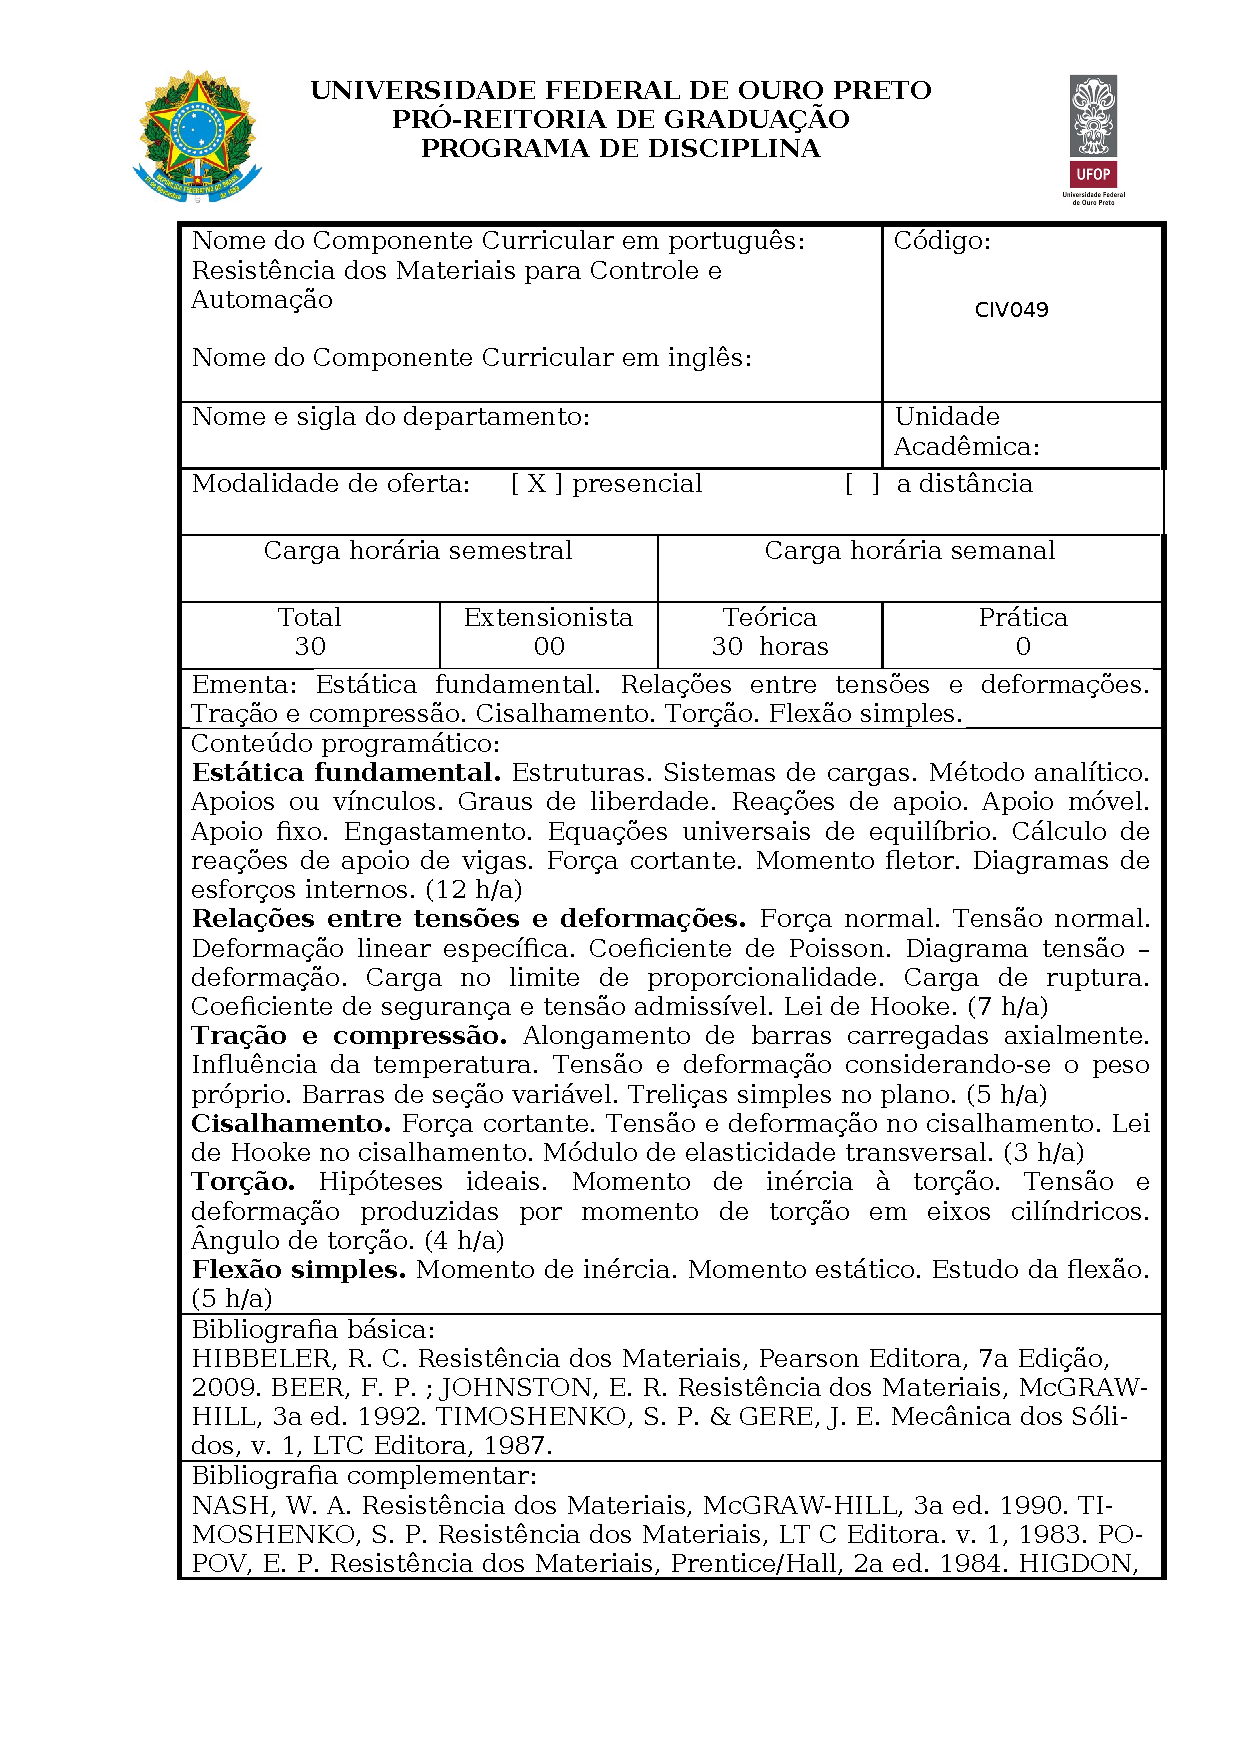
\includepdf[pages=-,nup=1x1, frame]{CIV049} %Resistência dos Materiais para Controle e Automação CIVXXX
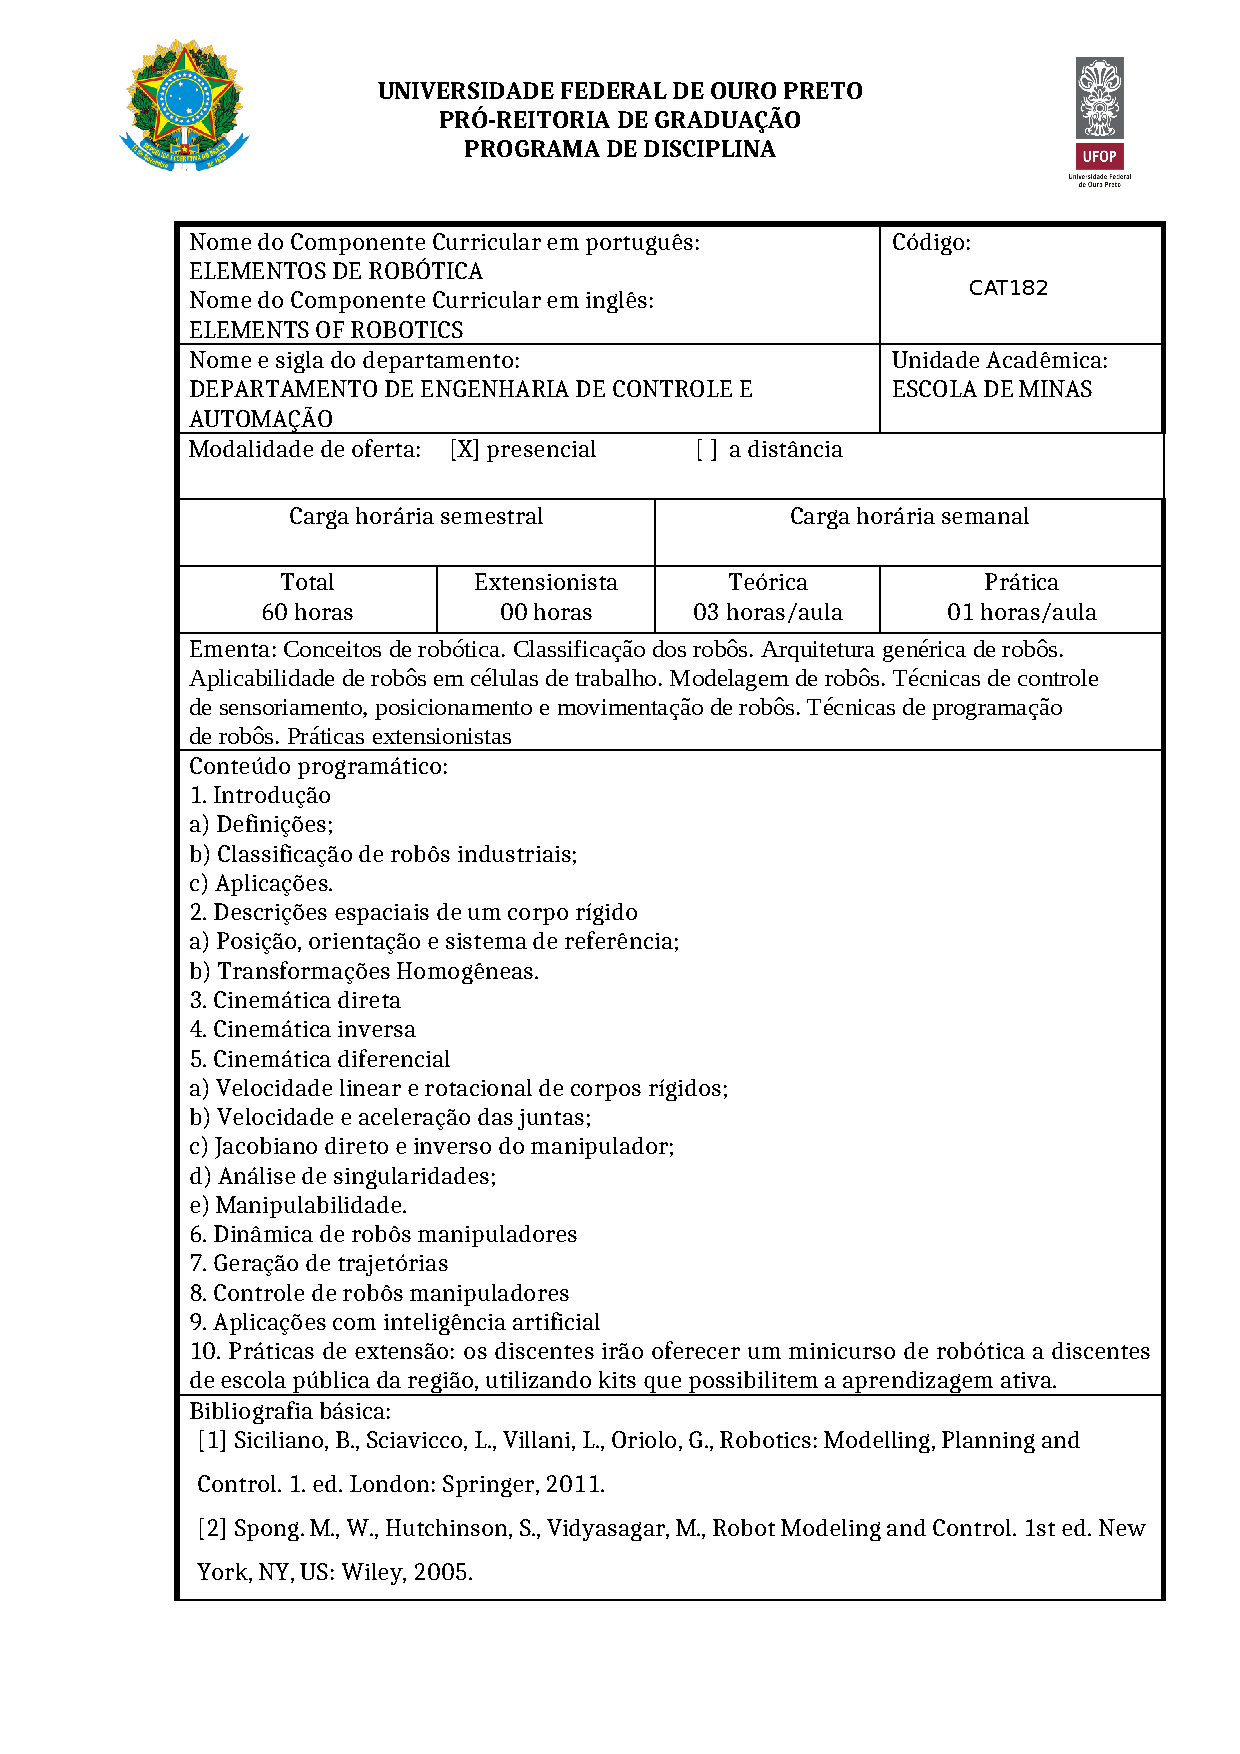
\includepdf[pages=-,nup=1x1, frame]{CAT182} %ELEMENTOS DE ROBÓTICA
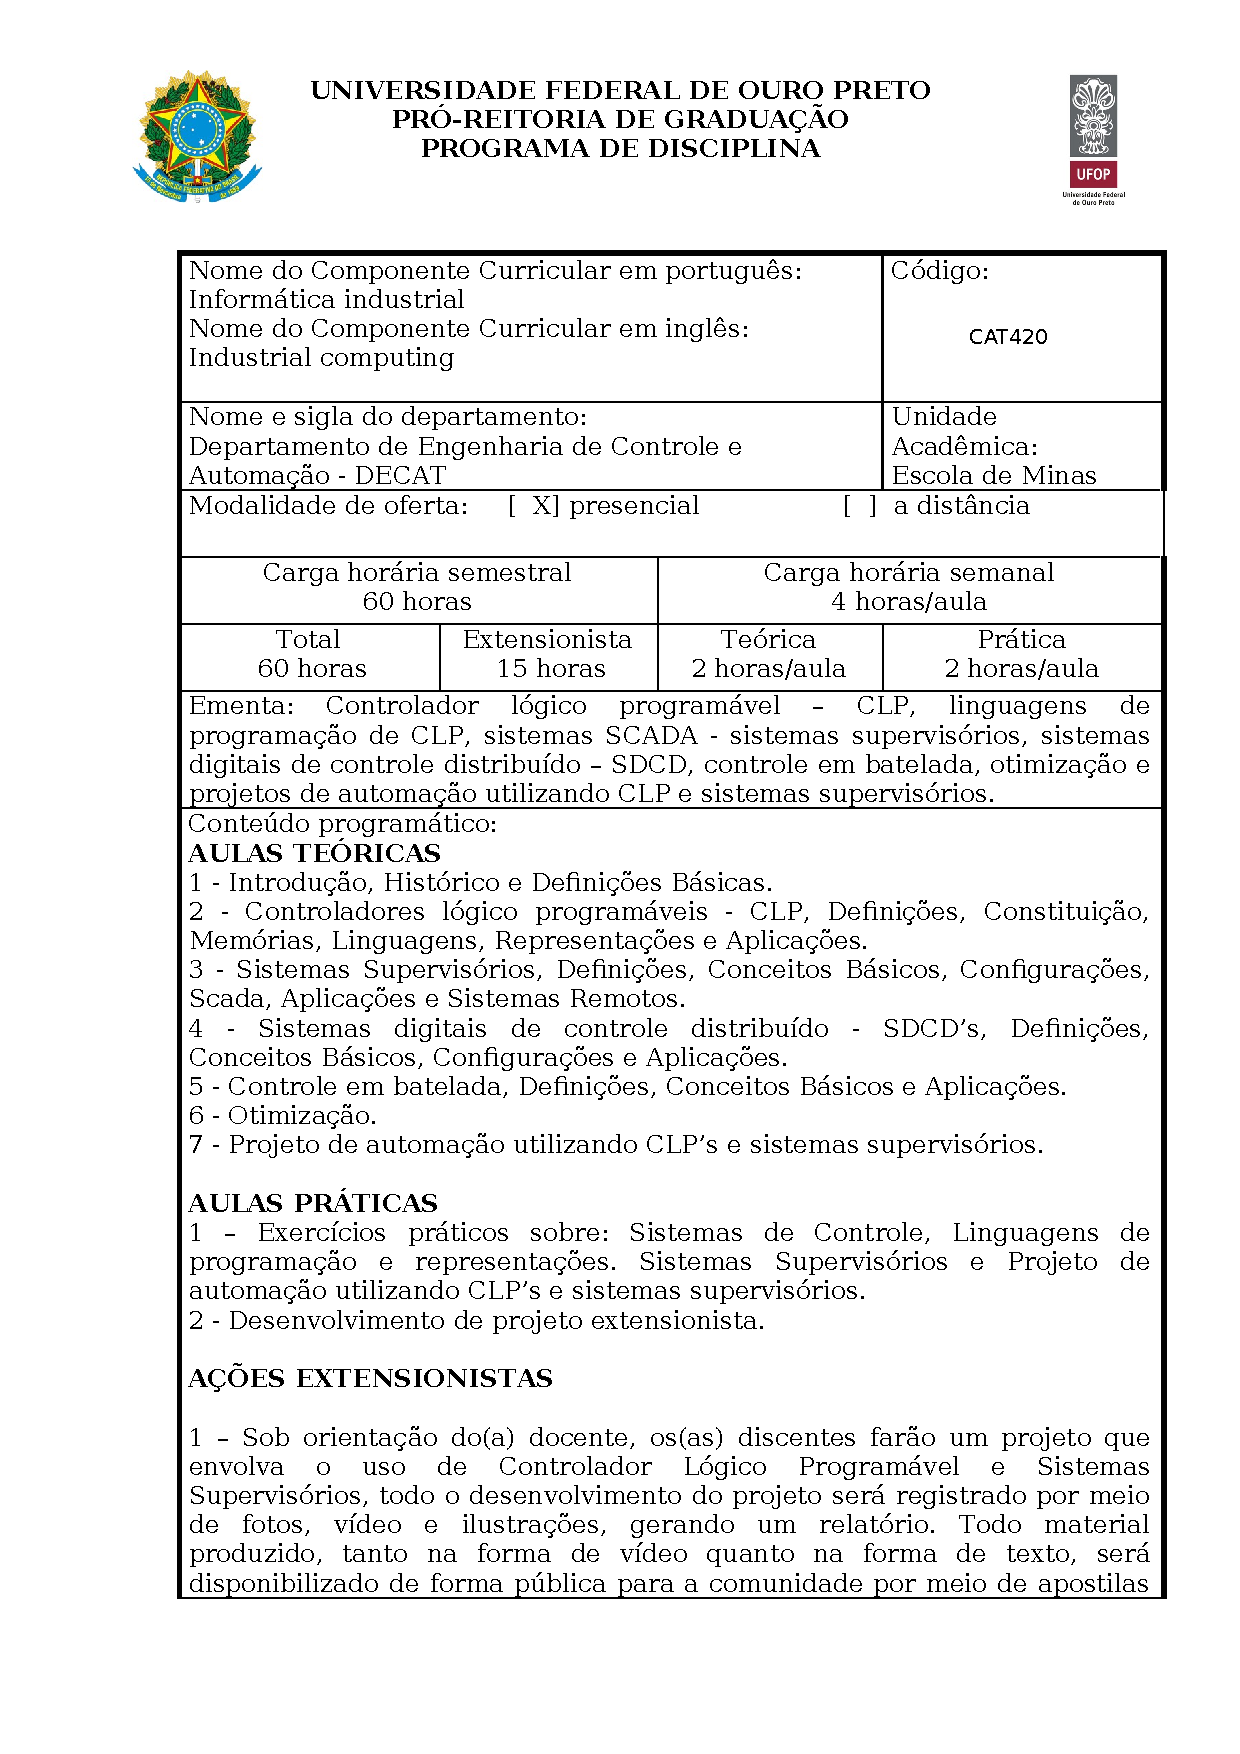
\includepdf[pages=-,nup=1x1, frame]{CAT420} %Informática industrial ANTIGA CAT175
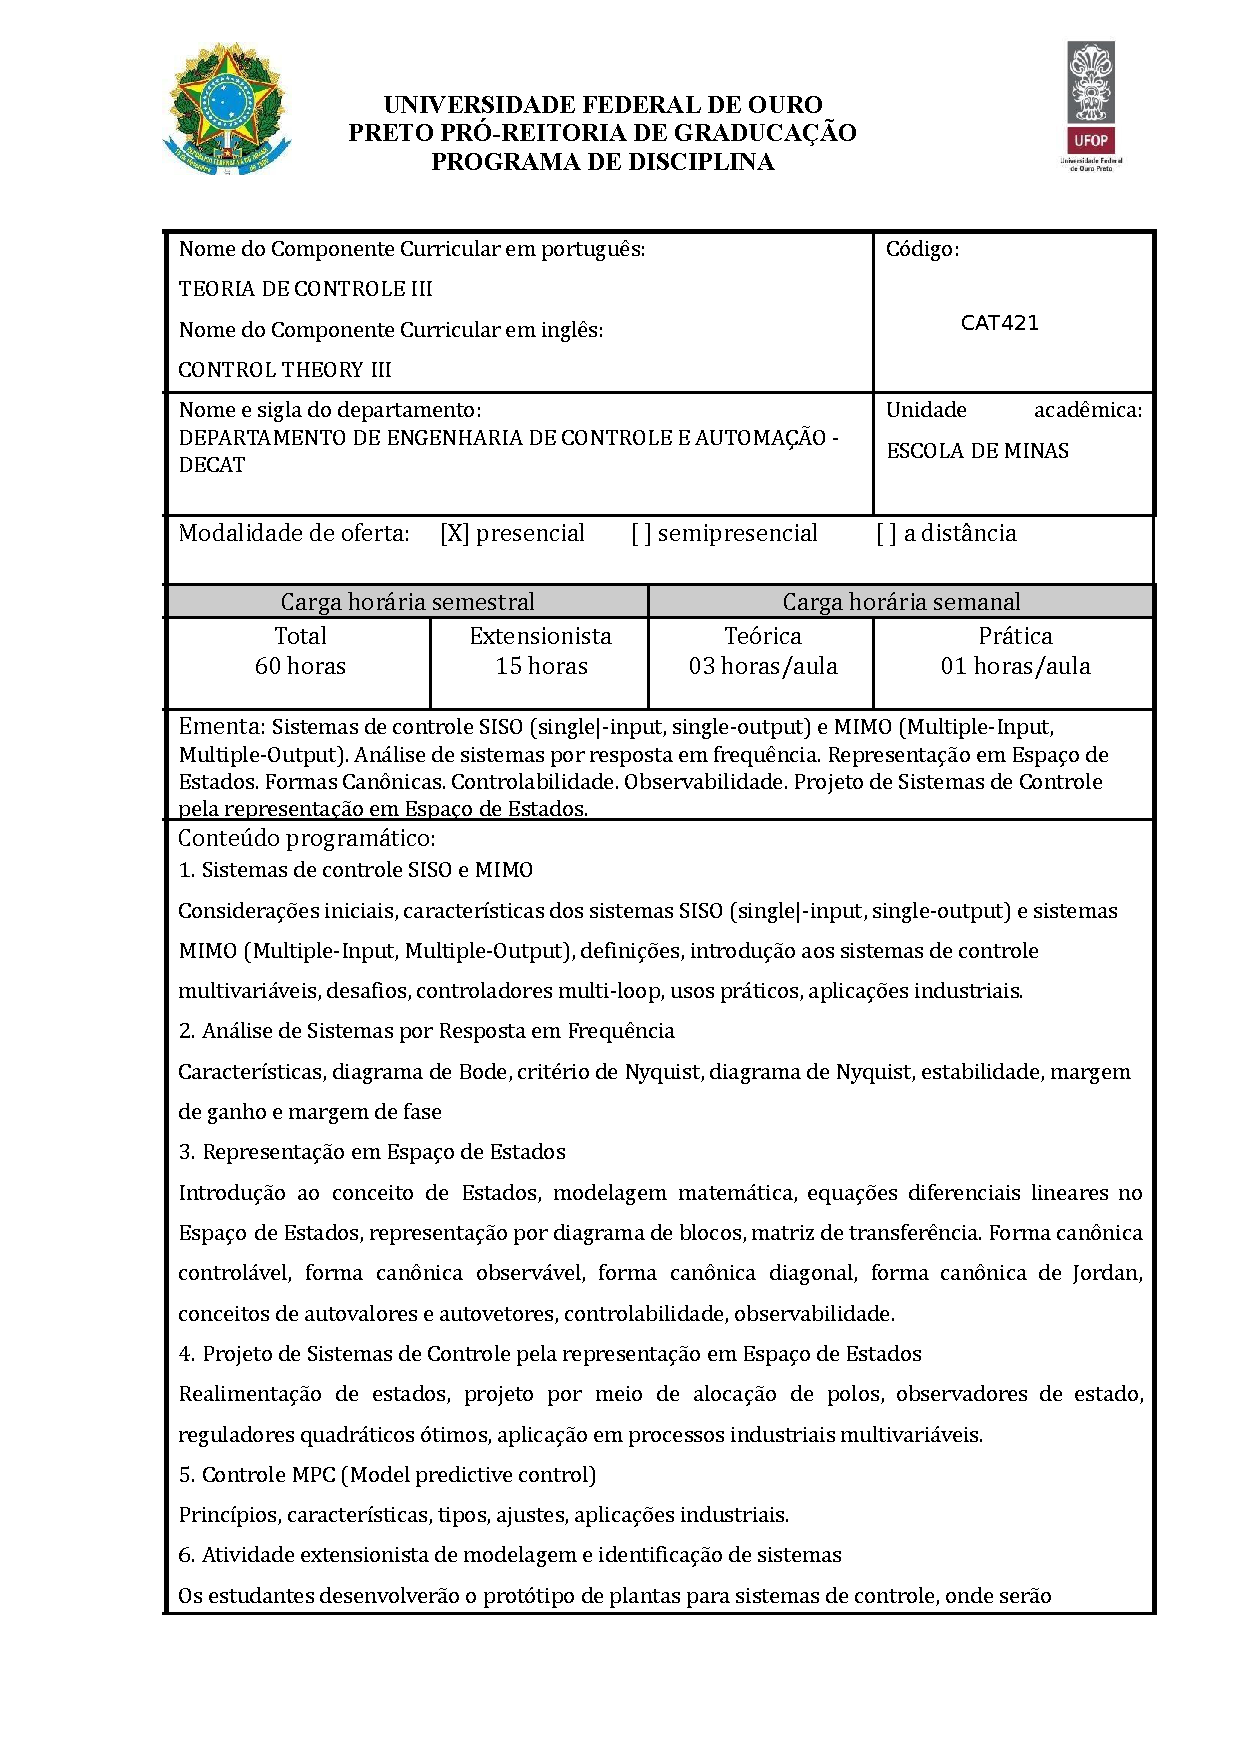
\includepdf[pages=-,nup=1x1, frame]{CAT421} %TEORIA DE CONTROLE III
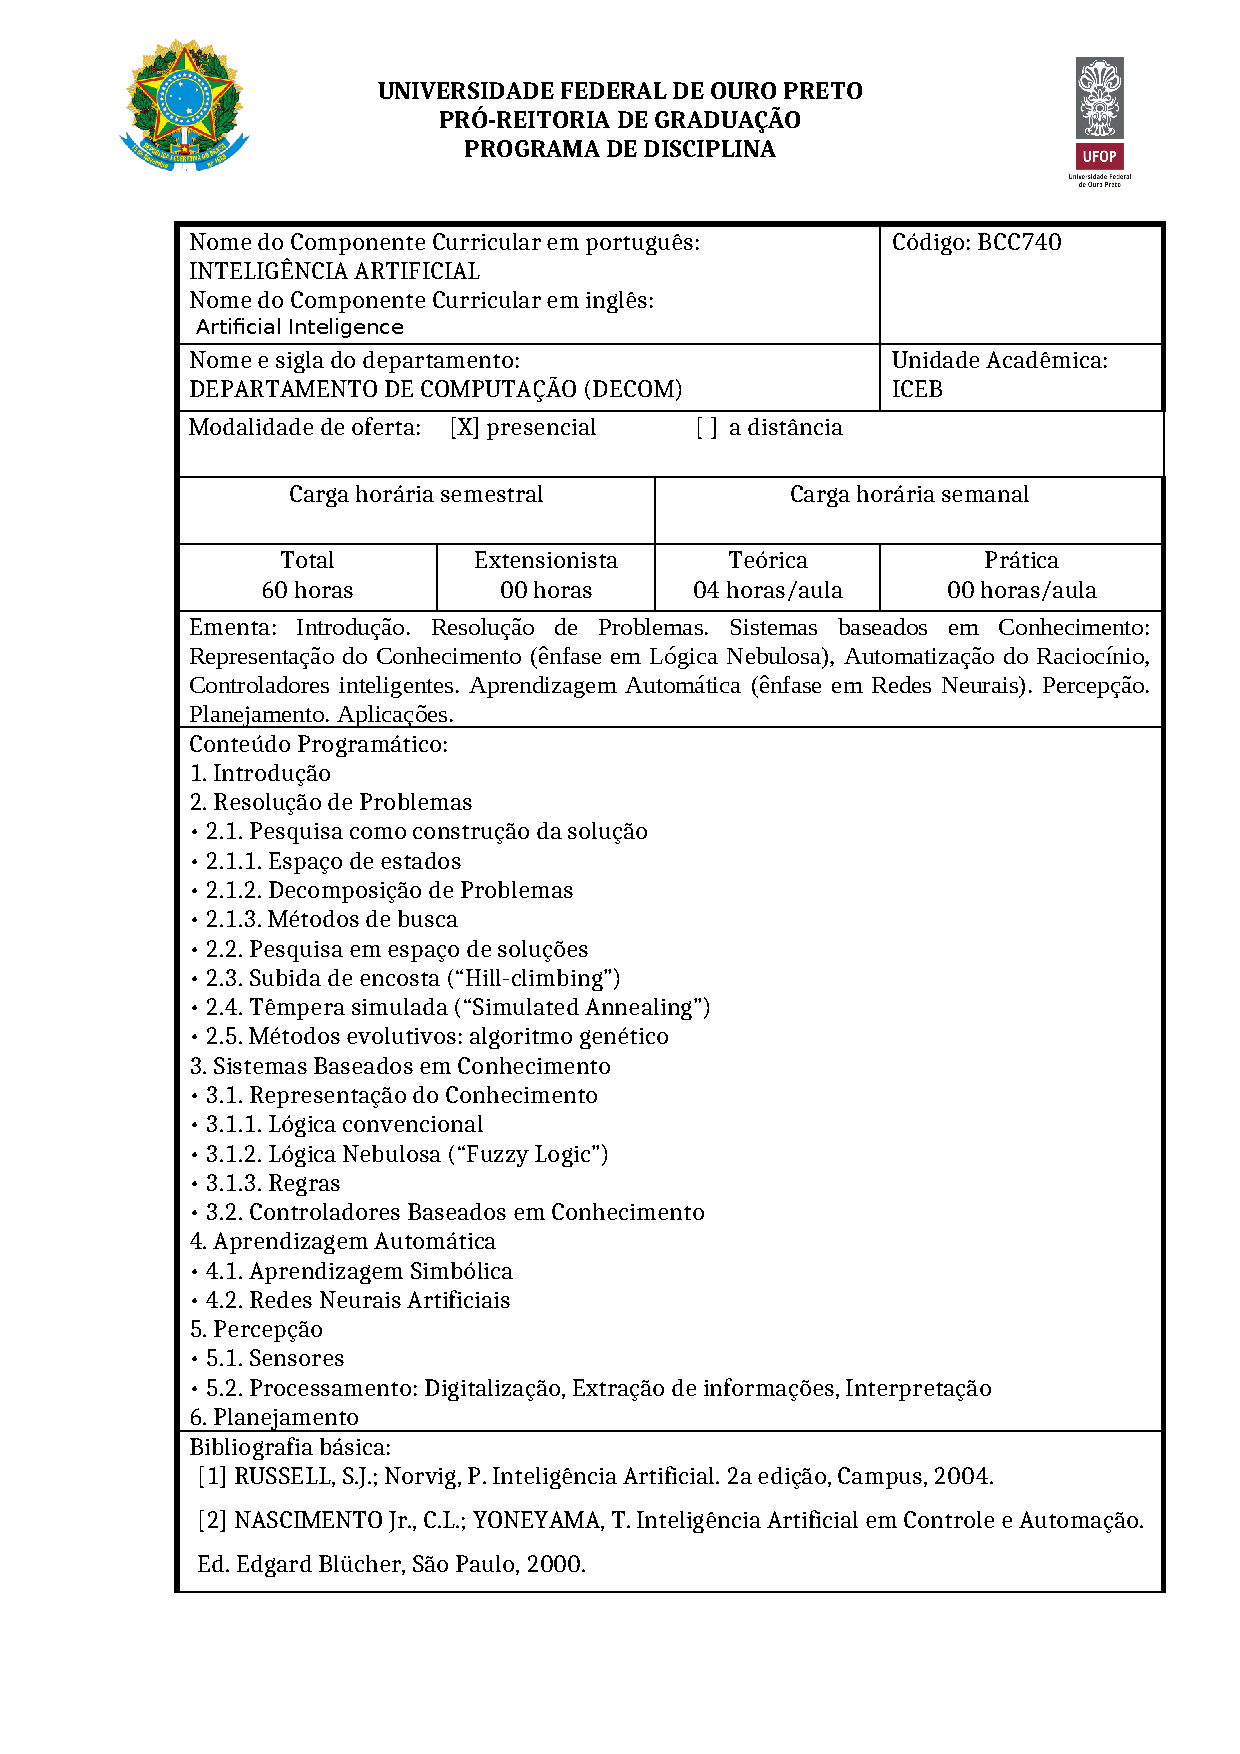
\includepdf[pages=-,nup=1x1, frame]{BCC740} %INTELIGENCIA ARTIFICIAL
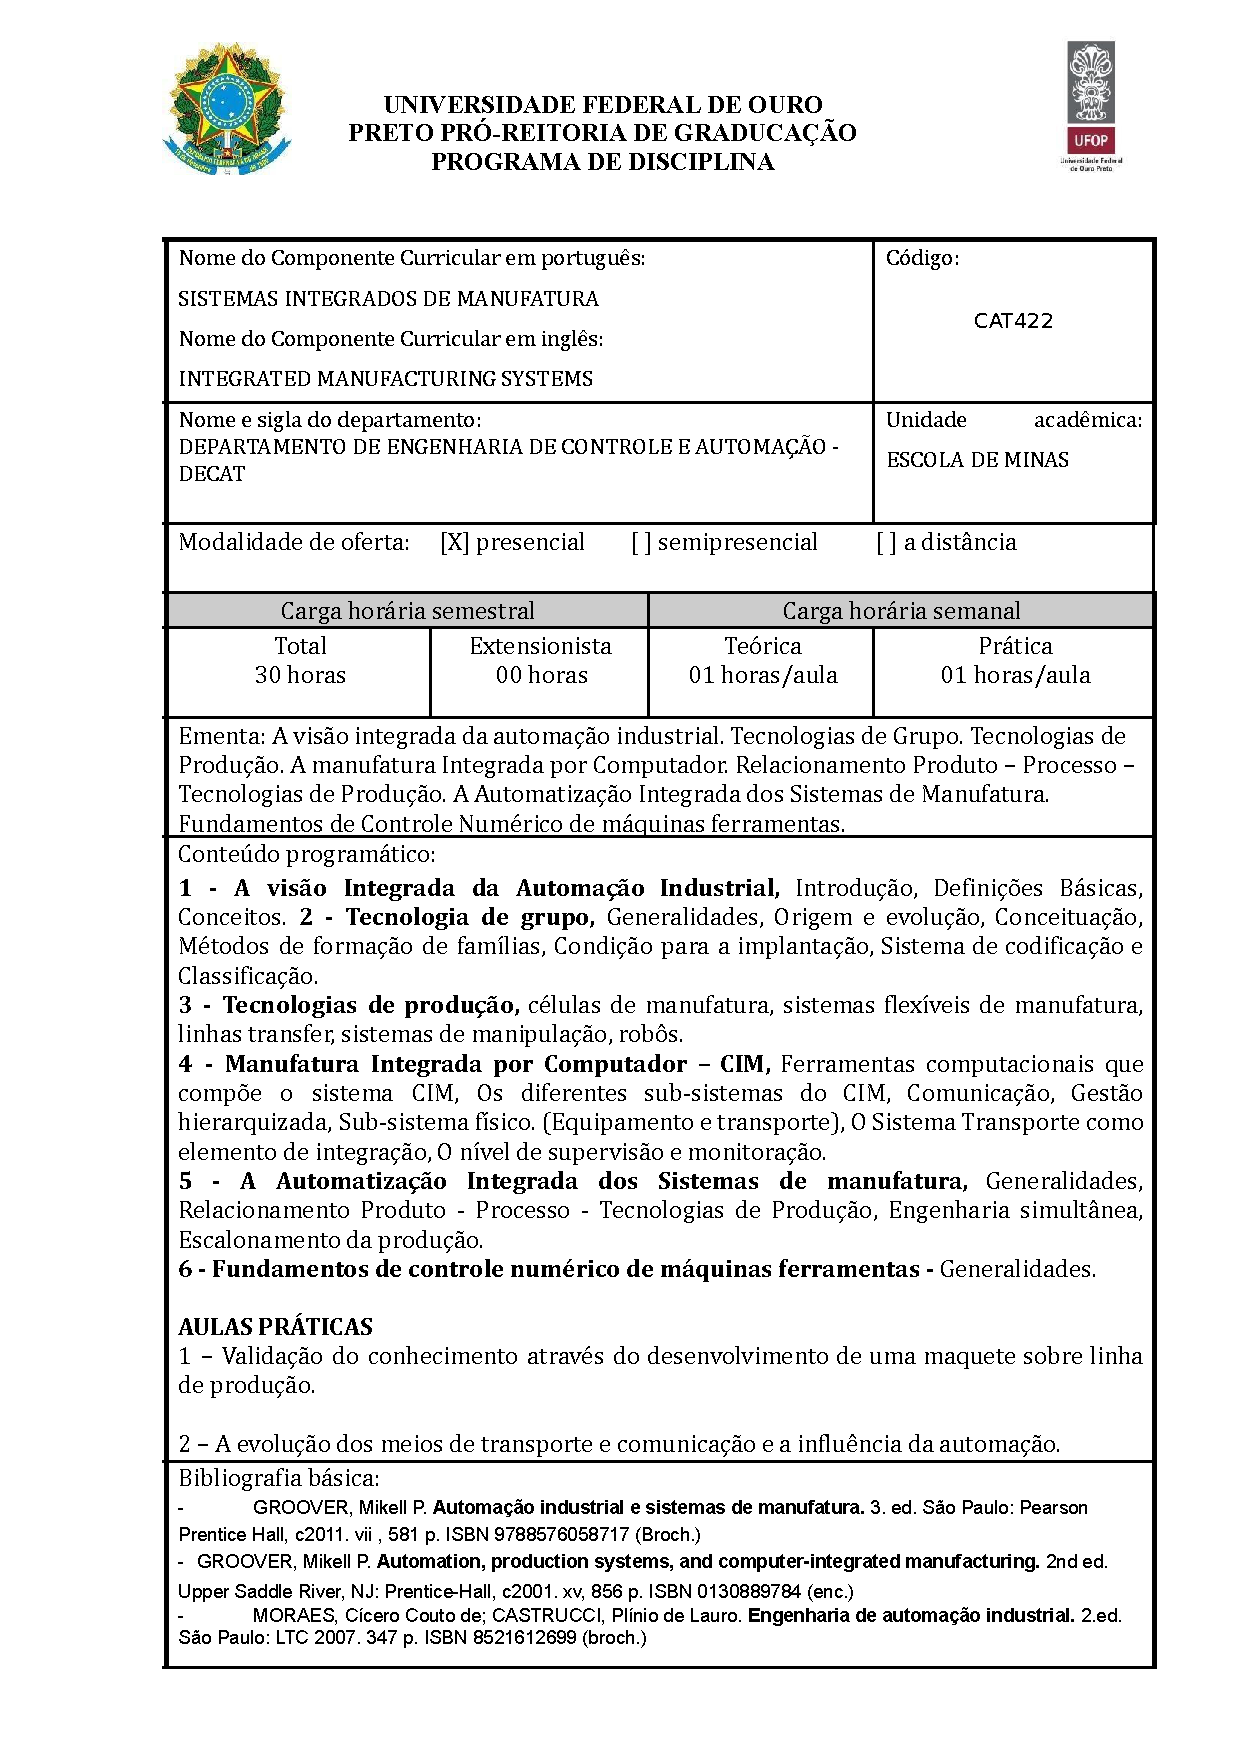
\includepdf[pages=-,nup=1x1, frame]{CAT422} %sistema integrado de manufatura XXX023

%Oitavo semestre
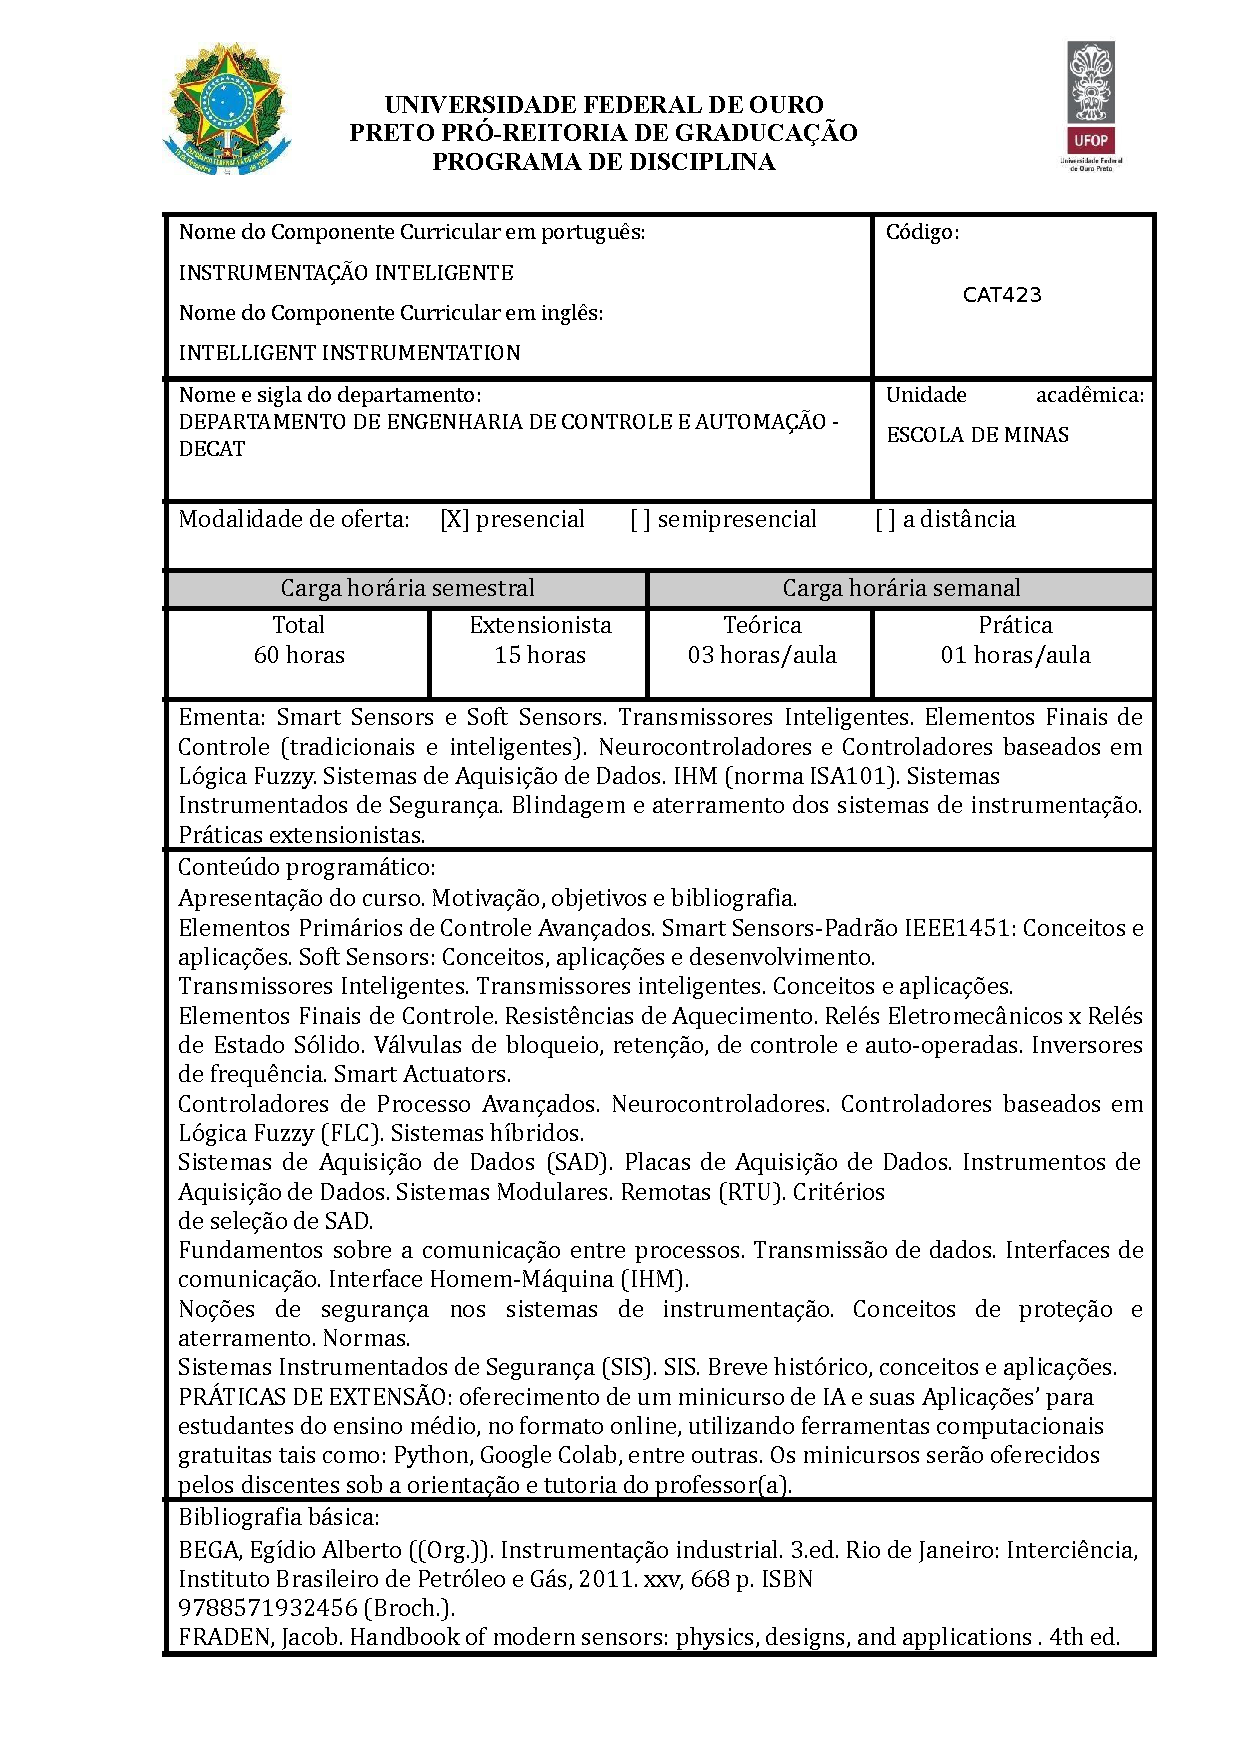
\includepdf[pages=-,nup=1x1, frame]{CAT423} % XXX013
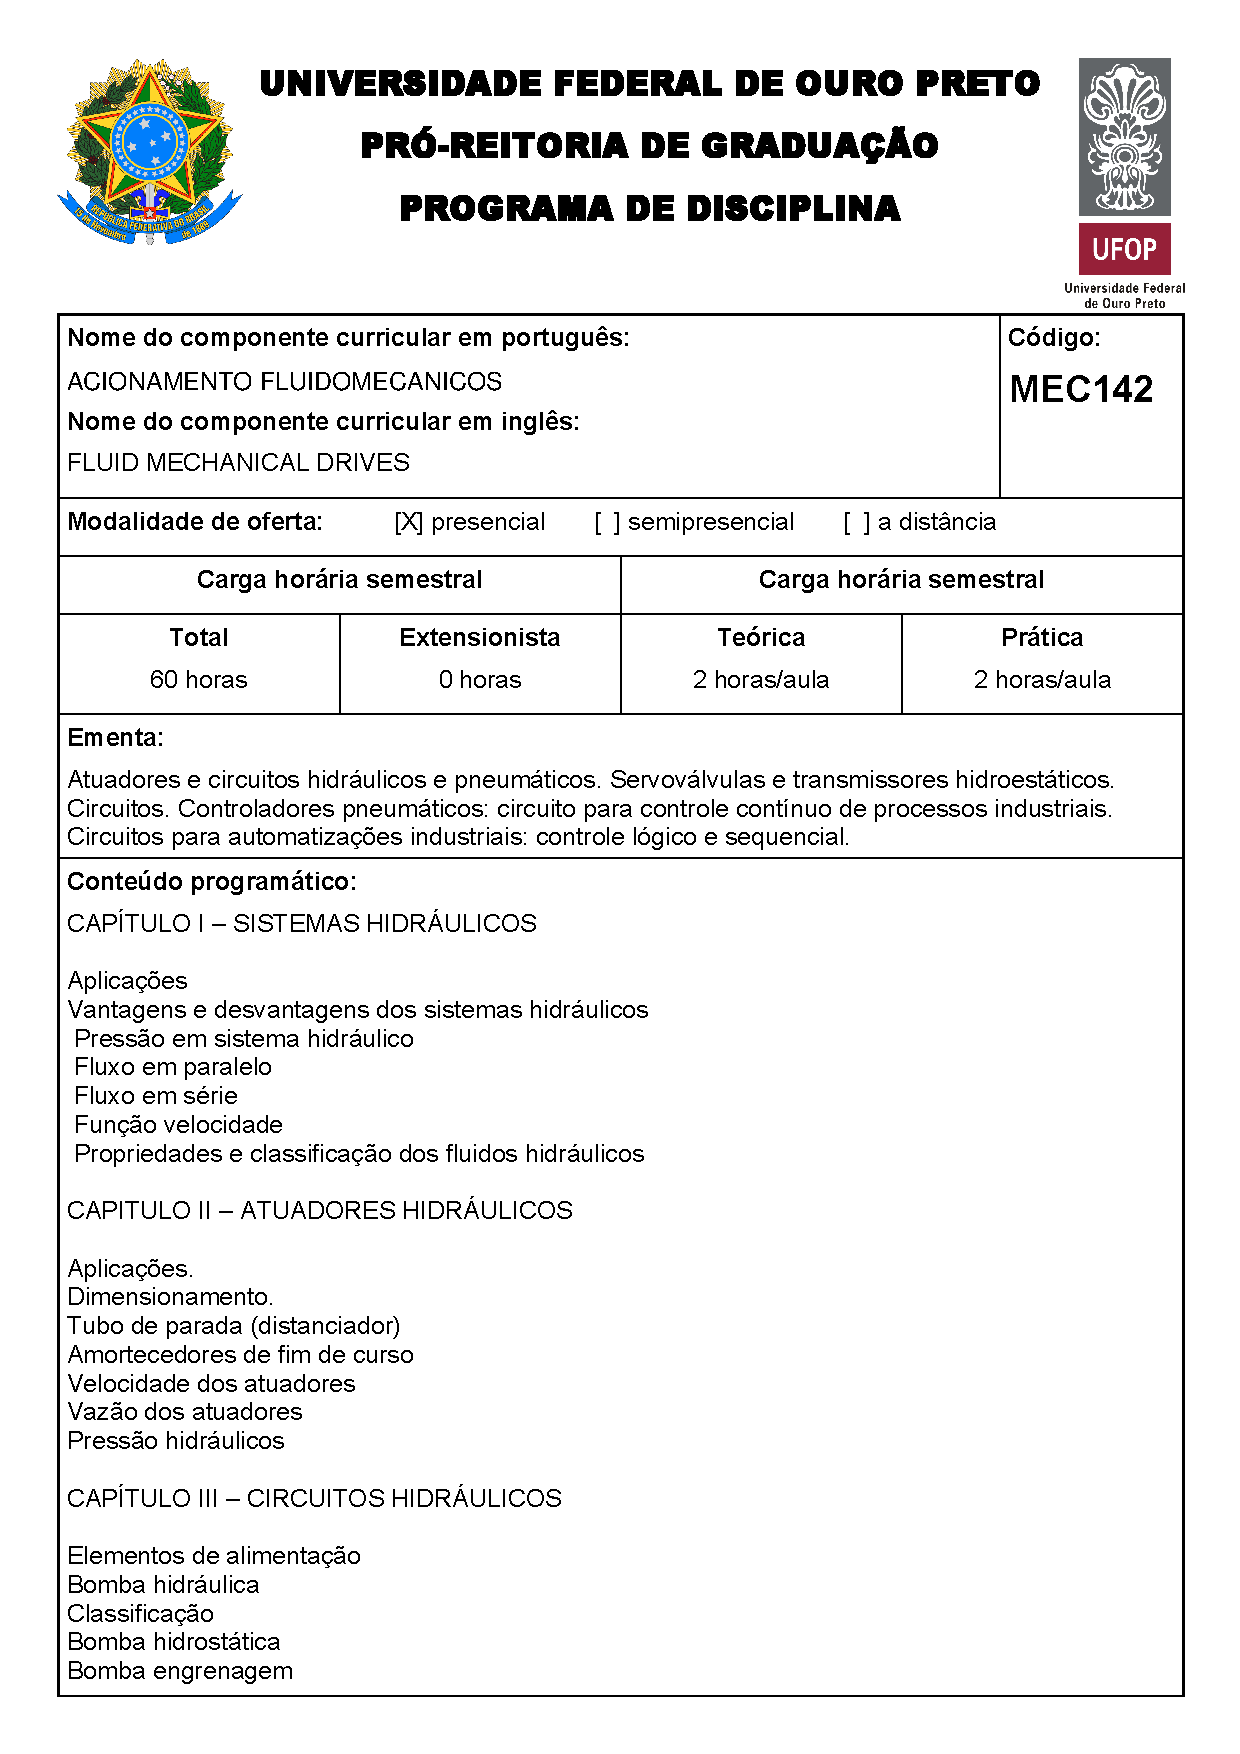
\includepdf[pages=-,nup=1x1, frame]{MEC142} %
\includepdf[pages=-,nup=1x1, frame]{CAT424} % XXX014
\includepdf[pages=-,nup=1x1, frame]{BCC722}


%Nono semestre
\includepdf[pages=-,nup=1x1, frame]{CAT425} % XXX015 (TFC1)
\includepdf[pages=-,nup=1x1, frame]{DIR250}
\includepdf[pages=-,nup=1x1, frame]{PRO224}
\includepdf[pages=-,nup=1x1, frame]{MIN107}
\includepdf[pages=-,nup=1x1, frame]{MET702}


%Decimo semestre
\includepdf[pages=-,nup=1x1, frame]{CAT491}
\includepdf[pages=-,nup=1x1, frame]{PRO243}
\includepdf[pages=-,nup=1x1, frame]{PRO215}

% eletivas
\includepdf[pages=-,nup=1x1, frame]{CAT426}
\includepdf[pages=-,nup=1x1, frame]{CAT427}
\includepdf[pages=-,nup=1x1, frame]{CAT428}
\includepdf[pages=-,nup=1x1, frame]{CAT429}
\includepdf[pages=-,nup=1x1, frame]{CAT430}
\includepdf[pages=-,nup=1x1, frame]{CAT437}
\includepdf[pages=-,nup=1x1, frame]{CAT438}
\includepdf[pages=-,nup=1x1, frame]{CAT178}
\includepdf[pages=-,nup=1x1, frame]{CAT432}
\includepdf[pages=-,nup=1x1, frame]{CAT433}
\includepdf[pages=-,nup=1x1, frame]{CAT341}
\includepdf[pages=-,nup=1x1, frame]{CAT434} 
\includepdf[pages=-,nup=1x1, frame]{CAT601}
\includepdf[pages=-,nup=1x1, frame]{CAT435} 
\includepdf[pages=-,nup=1x1, frame]{BCC408}
\includepdf[pages=-,nup=1x1, frame]{BCC406}
\includepdf[pages=-,nup=1x1, frame]{BCC264}
\includepdf[pages=-,nup=1x1, frame]{BCC321}
\includepdf[pages=-,nup=1x1, frame]{BCC326}
\includepdf[pages=-,nup=1x1, frame]{BCC362}
\includepdf[pages=-,nup=1x1, frame]{BCC503}
\includepdf[pages=-,nup=1x1, frame]{BCC221}
\includepdf[pages=-,nup=1x1, frame]{BCC263}
\includepdf[pages=-,nup=1x1, frame]{CSO010}
\includepdf[pages=-,nup=1x1, frame]{FIL652}
\includepdf[pages=-,nup=1x1, frame]{LET041}
\includepdf[pages=-,nup=1x1, frame]{MEC104}
\includepdf[pages=-,nup=1x1, frame]{MEC108}
\includepdf[pages=-,nup=1x1, frame]{PRO302}
\includepdf[pages=-,nup=1x1, frame]{PRO706}
\includepdf[pages=-,nup=1x1, frame]{CAT436}
\includepdf[pages=-,nup=1x1, frame]{PRO725}
\chapter{Resoluções CECAU} \label{resolucoes-cecau}

\includepdf[pages=-,nup=1x1, frame]{CECAU01}
\includepdf[pages=-,nup=1x1, frame]{CECAU02}
\includepdf[pages=-,nup=1x1, frame]{CECAU03}
\includepdf[pages=-,nup=1x1, frame]{CECAU04}
%\end{comment}

\end{anexosenv}

%%%%%%%%%%%%%%%%%%%%%%%%%%%%%%%%%%%%%%%%%%%%%%%%%%%%%%%%%%%%%%%%%%%%%%%%%%%%comentado até aqui
%% Glossario
%\renewcommand{\glossaryname}{Glossário}
%\renewcommand{\glossarypreamble}{Esta é a descrição do glossário.}
% ---
% Traduções para o ambiente glossaries
% ---
%\providetranslation{Glossary}{Glossário}
% ---
% ---
% Estilo de glossário
 %\setglossarystyle{tree}
% ---
% Imprime o glossário
% ---
%\cleardoublepage
% \phantomsection
% \addcontentsline{toc}{chapter}{\glossaryname}
% \printglossaries
% ---

%---------------------------------------------------------------------
% INDICE REMISSIVO
%---------------------------------------------------------------------
\printindex
\end{document}
